\documentclass[letterpaper,12pt,twoside=false,DIV=11]{scrbook}

%----------------------CONFIG---------------------------
%math packages
\usepackage{amsmath,amssymb,amsthm,units,unitsdef}
\usepackage{wasysym}  % astro symbols

%bibliography style and citation style, bibstyles to use: plainnat, abbrvnat, unsrtnat, named, chicago
%otherwise numerical citationstyle will be used
\usepackage[authoryear,round]{natbib}
\usepackage{longtable,tabularx,tabulary,multirow,lscape}
\usepackage[font={sl},format=plain,labelfont=bf]{caption}

% appendix
\usepackage{appendix}
\usepackage{xpatch}
\xpretocmd{\appendixpagename}{\sffamily}{}{}

% colors
\usepackage{color,colortbl}
\usepackage[dvipsnames]{xcolor}
\definecolor{darkblue}{HTML}{00354C}

\usepackage{booktabs}
% \usepackage{showkeys} % shows the labels above the references for

%easier development
\usepackage{ifpdf}

\ifpdf
	\usepackage[pdftex]{graphicx}
	\usepackage[]{pdfpages} %for including full pdf pages
	\usepackage[pdftex,
		bookmarks,
		bookmarksopen=true,
		bookmarksnumbered=true,
		pdfauthor={Reto Trappitsch},
		pdftitle={On the origin of elements in the Milky Way},
		colorlinks,
		linkcolor=darkblue,
		citecolor=darkblue,
		filecolor=black,
		urlcolor=darkblue,
		anchorcolor=black,
		menucolor=black,
		breaklinks=true,
		pageanchor=true, %for jumping to a page
		plainpages=false,
		pdfpagelabels=true,
		breaklinks=true]{hyperref}
	\pdfcompresslevel=9
	\pdfoutput=1
	\DeclareGraphicsExtensions{.pdf,.png,.jpg,.jpeg}
\else
	\usepackage{graphicx}
\fi
\usepackage{rotating} % rotate figures
\usepackage{subcaption}
\usepackage{wrapfig}

% break URLs at -
\def\UrlBreaks{\do\/\do-}

%page style
%==========
%\usepackage{geometry}
%\geometry{top=1.0in, bottom=1.0in, left=1.0in, right=1.0in,footskip = 0.5in} 

% Alert boxes
\usepackage{awesomebox}

% Acronyms
\usepackage{acro}
\acsetup{
	make-links = true
}
% THIS FILE CANNOT BE COMPILED ALONE.

% Declare acronyms below in alphabetical order to use with \usepackage{acro}. 

% DECLARE ACRONYMS %

% NUMBERS
\DeclareAcronym{1d}{short = 2D, long = 1 dimensional}
\DeclareAcronym{2d}{short = 2D, long = 2 dimensional}
\DeclareAcronym{3d}{short = 3D, long = 3 dimensional}

% A
\DeclareAcronym{au}{short = AU, long = astronomical unit, short-plural-form=AU}

% B
\DeclareAcronym{bbn}{short = BBN, long = Big Bang nucleosynthesis}

% C
\DeclareAcronym{cai}{short = CAI, long = calcium-aluminum-rich inclusion}
\DeclareAcronym{ccsn}{short = CCSN, long = core-collapse supernova, short-plural = e, long-plural = e}
\DeclareAcronym{chili}{short = CHILI, long = Chicago instrument for laser ionization}
\DeclareAcronym{cmb}{short = CMB, long = cosmic microwave background}
\DeclareAcronym{cre}{short = CRE, long = cosmic ray exposure}

% D
\DeclareAcronym{dex}{short = dex, long = decimal exponent}
\DeclareAcronym{doi}{short = doi, long = digital object identifier}

% E
\DeclareAcronym{ecsn}{short = ECSN, long = electron-capture supernova, short-plural = e, long-plural = e}
\DeclareAcronym{euv}{short = EUV, long = extreme ultraviolet}

% F
\DeclareAcronym{fip}{short = FIP, long = first ionization potential}
\DeclareAcronym{fit}{short = FIT, long = first ionization time}

% G
\DeclareAcronym{gce}{short = GCE, long = galactic chemical evolution}
\DeclareAcronym{gcr}{short = GCR, long = galactic cosmic ray}
\DeclareAcronym{gw}{short = GW, long = gravitational wave}

% H
\DeclareAcronym{hst}{short = HST, long = Hubble Space Telescope}

% I
\DeclareAcronym{icpms}{short = ICP-MS, long = inductively coupled plasma mass spectrometry}
\DeclareAcronym{imf}{short = IMF, long = initial mass function}
% \DeclareAcronym{imf}{short = IMF, long = instrumental mass fractionation}
\DeclareAcronym{ir}{short = IR, long = infrared radiation}
\DeclareAcronym{ism}{short = ISM, long = interstellar medium}

% J

% K

% L
\DeclareAcronym{ligo}{short = LIGO, long = laser interferometer gravitational-wave observatory}
\DeclareAcronym{lion}{short = LION, long = laser ionization of neutrals}
\DeclareAcronym{lte}{short = LTE, long = local thermodynamic equilibrium}

% M
\DeclareAcronym{mesa}{short = MESA, long = Modules for Experiments in Stellar Astrophysics}
\DeclareAcronym{mc}{short = MC, long = Monte Carlo}
\DeclareAcronym{mswd}{short = MSWD, long = mean square weighted deviation}

% N
\DeclareAcronym{nanosims}{short = NanoSIMS, long = nanoscale secondary ion mass spectrometry}
\DeclareAcronym{nlte}{short = NLTE, long = nonplocal thermodynamic equilibrium}
\DeclareAcronym{ns}{short = NS, long = neutron star}

% O
\DeclareAcronym{odr}{short = ODR, long = orthogonal distance regression}

% P
\DeclareAcronym{pc}{short = pc, long = parsec}
\DeclareAcronym{pdf}{short = pdf, long = portable document format}
\DeclareAcronym{pdfstat}{short = PDF, long = probability density function}

% Q

% R
\DeclareAcronym{rims}{short = RIMS, long = resonance ionization mass spectrometry}
\DeclareAcronym{rproc}{short = \textit{r}-process, long = rapid neutron capture process, short-plural = es, long-plural = es}
\DeclareAcronym{rsf}{short = RSF, long = relative sensitivity factor}

% S
\DeclareAcronym{scr}{short = SCR, long = solar cosmic ray}
\DeclareAcronym{sep}{short = SEP, long = solar energetic particle}
\DeclareAcronym{slr}{short = SLR, long = short-lived radionuclide}
\DeclareAcronym{sfr}{short = SFR, long = star formation rate}
\DeclareAcronym{sims}{short = SIMS, long = secondary ion mass spectrometry}
\DeclareAcronym{soho}{short = SOHO, long = solar and heliospheric observatory}
\DeclareAcronym{sn}{short = SN, long = supernova, short-plural = e, long-plural = e}
\DeclareAcronym{snia}{short = SN-Ia, long = type Ia supernova, short-plural-form = SNe-Ia, long-plural = e}
\DeclareAcronym{snii}{short = SN-II, long = type II supernova, short-plural-form = SNe-II, long-plural = e}
\DeclareAcronym{sproc}{short = \textit{s}-process, long = slow neutron capture process, short-plural = es, long-plural = es}
\DeclareAcronym{sw}{short = SW, long = solar wind}

% T
\DeclareAcronym{tof}{short = TOF, long = time-of-flight}

% U
\DeclareAcronym{uv}{short = UV, long = ultraviolet}

% V

% W
\DeclareAcronym{wd}{short = WD, long = white dwarf}
\DeclareAcronym{wmap}{short = WMAP, long = Wilkinson microwave anisotropy probe}

% X

% Y

% Z

% newcommands
%============
% my short cuts
\providecommand{\e}[1]{\ensuremath{\times 10^{#1}}}
\providecommand{\ex}[1]{\ensuremath{^{#1}}}
\providecommand{\dex}[1]{\ensuremath{\delta^{#1}}}
\newcommand{\nean}{$^{22}$Ne($\alpha$,n)$^{25}$Mg}

% textnormal
\newcommand{\tn}{\textnormal}
% textregistered
\newcommand{\tr}{$^\tn{\textregistered}$}

% more box stuff
\makeatletter
\providecommand{\boxtitle}[1]{\sffamily{\textbf{#1}}\normalfont}
	
\providecommand{\infobox}[2]{\awesomebox[MidnightBlue]{2pt}{\faPaw}{MidnightBlue}{\boxtitle{#1} #2}}
\providecommand{\morebox}[2]{\awesomebox[BrickRed]{2pt}{\faRocket}{BrickRed}{\boxtitle{#1} #2}}
\providecommand{\codebox}[2]{\awesomebox[OliveGreen]{2pt}{\faCode}{OliveGreen}{\boxtitle{#1} #2}}



%======================================================
%title specifications

\title{On the Origin of Elements in the Milky Way}
\author{Reto Trappitsch}
\date{Spring semester 2021}

%======================================================
% UPDATES %
%======================================================
% exoplanets
\newcommand{\ExoplanetsNumber}{4352}  % confirmed
\newcommand{\ExoplanetDate}{February 26, 2021}

%======================================================




%-------------------DOCUMENT---------------------------

\usepackage{blindtext}
\begin{document}

\maketitle
% TOC
\pagenumbering{roman}
\setcounter{page}{1}
\tableofcontents

\clearpage


% MAIN TEXT
\pagenumbering{arabic}
\setcounter{page}{1}

\chapter*{Preface}\label{sec:preface}
\addcontentsline{toc}{chapter}{Preface}

These lecture notes for the course ``On the origin of the elements in the Milky Way'' are prepared as we go, so they will be in part influenced by you! If you find typos, errors, or other issues please let me know. The most recent copy of the \LaTeX\ files and figures can also be found on \href{https://github.com/galactic-forensics/lecutre_origin_elements/}{GitHub}.

The lecture notes contain clickable links, e.g., all references are linked to the bibliography and all acronyms are linked to the acronyms' definition page. These links are generally colored in \textcolor{darkblue}{dark blue}.

The end of the document contains a bibliography that contains details on all references. Note that references here are limited and often point to review articles that could be of interest to the reader. More detailed references to individual topics can be found in these articles. Each reference entry contains a \acf{doi}\footnote{\url{https://doi.org}} that can be found online and accessed via a Brandeis library subscription. Alternatively, a link to ArXiV\footnote{\url{https://arxiv.org}} is provided.

Specific boxes throughout the text discuss further information. They are defined as following:

\infobox{Background information}{on topics that do not necessarily fit into the text but are important to keep in mind will be given in a box like this.}

\morebox{Further information and reading}{for the avid reader will be pointed out in a box like this. The scope of these boxes is generally slightly outside the realm of the class.}

\codebox{Programming}{is an integral part of scientific research, be it for running experiments, performing measurements, evaluating measurements, or modeling a system. A box like this will point you to more information with respect to coding. These boxes will often refer to coding in \href{https://www.python.org}{python}.}

\printacronyms


% Chapters

%!TEX root = origin_elements_lecture_notes.tex

\chapter{Solar System Abundances}\label{ch:solar_system_abundances}

To understand the origin of the elements in the Milky Way, it is crucial to first understand what in fact needs explaining. One of the best studied points in the history of the Milky Way is the Solar System we inhabit, mainly since we actually live inside it and thus have direct access to its material.

The Solar System formed 4.567\,Ga ago from a homogeneous molecular cloud. Since the Milky Way itself formed roughly 13\,Ga ago, the molecular cloud from which the solar nebula formed evolved for roughly 8.4\,Ga since the formation of the Milky Way and around 9\,Ga since the Big Bang. The process that describes the formation and destruction of elements over this period of time is generally referred to as \ac{gce}. 

\begin{figure}[bt]
    \begin{subfigure}{0.5\textwidth}
        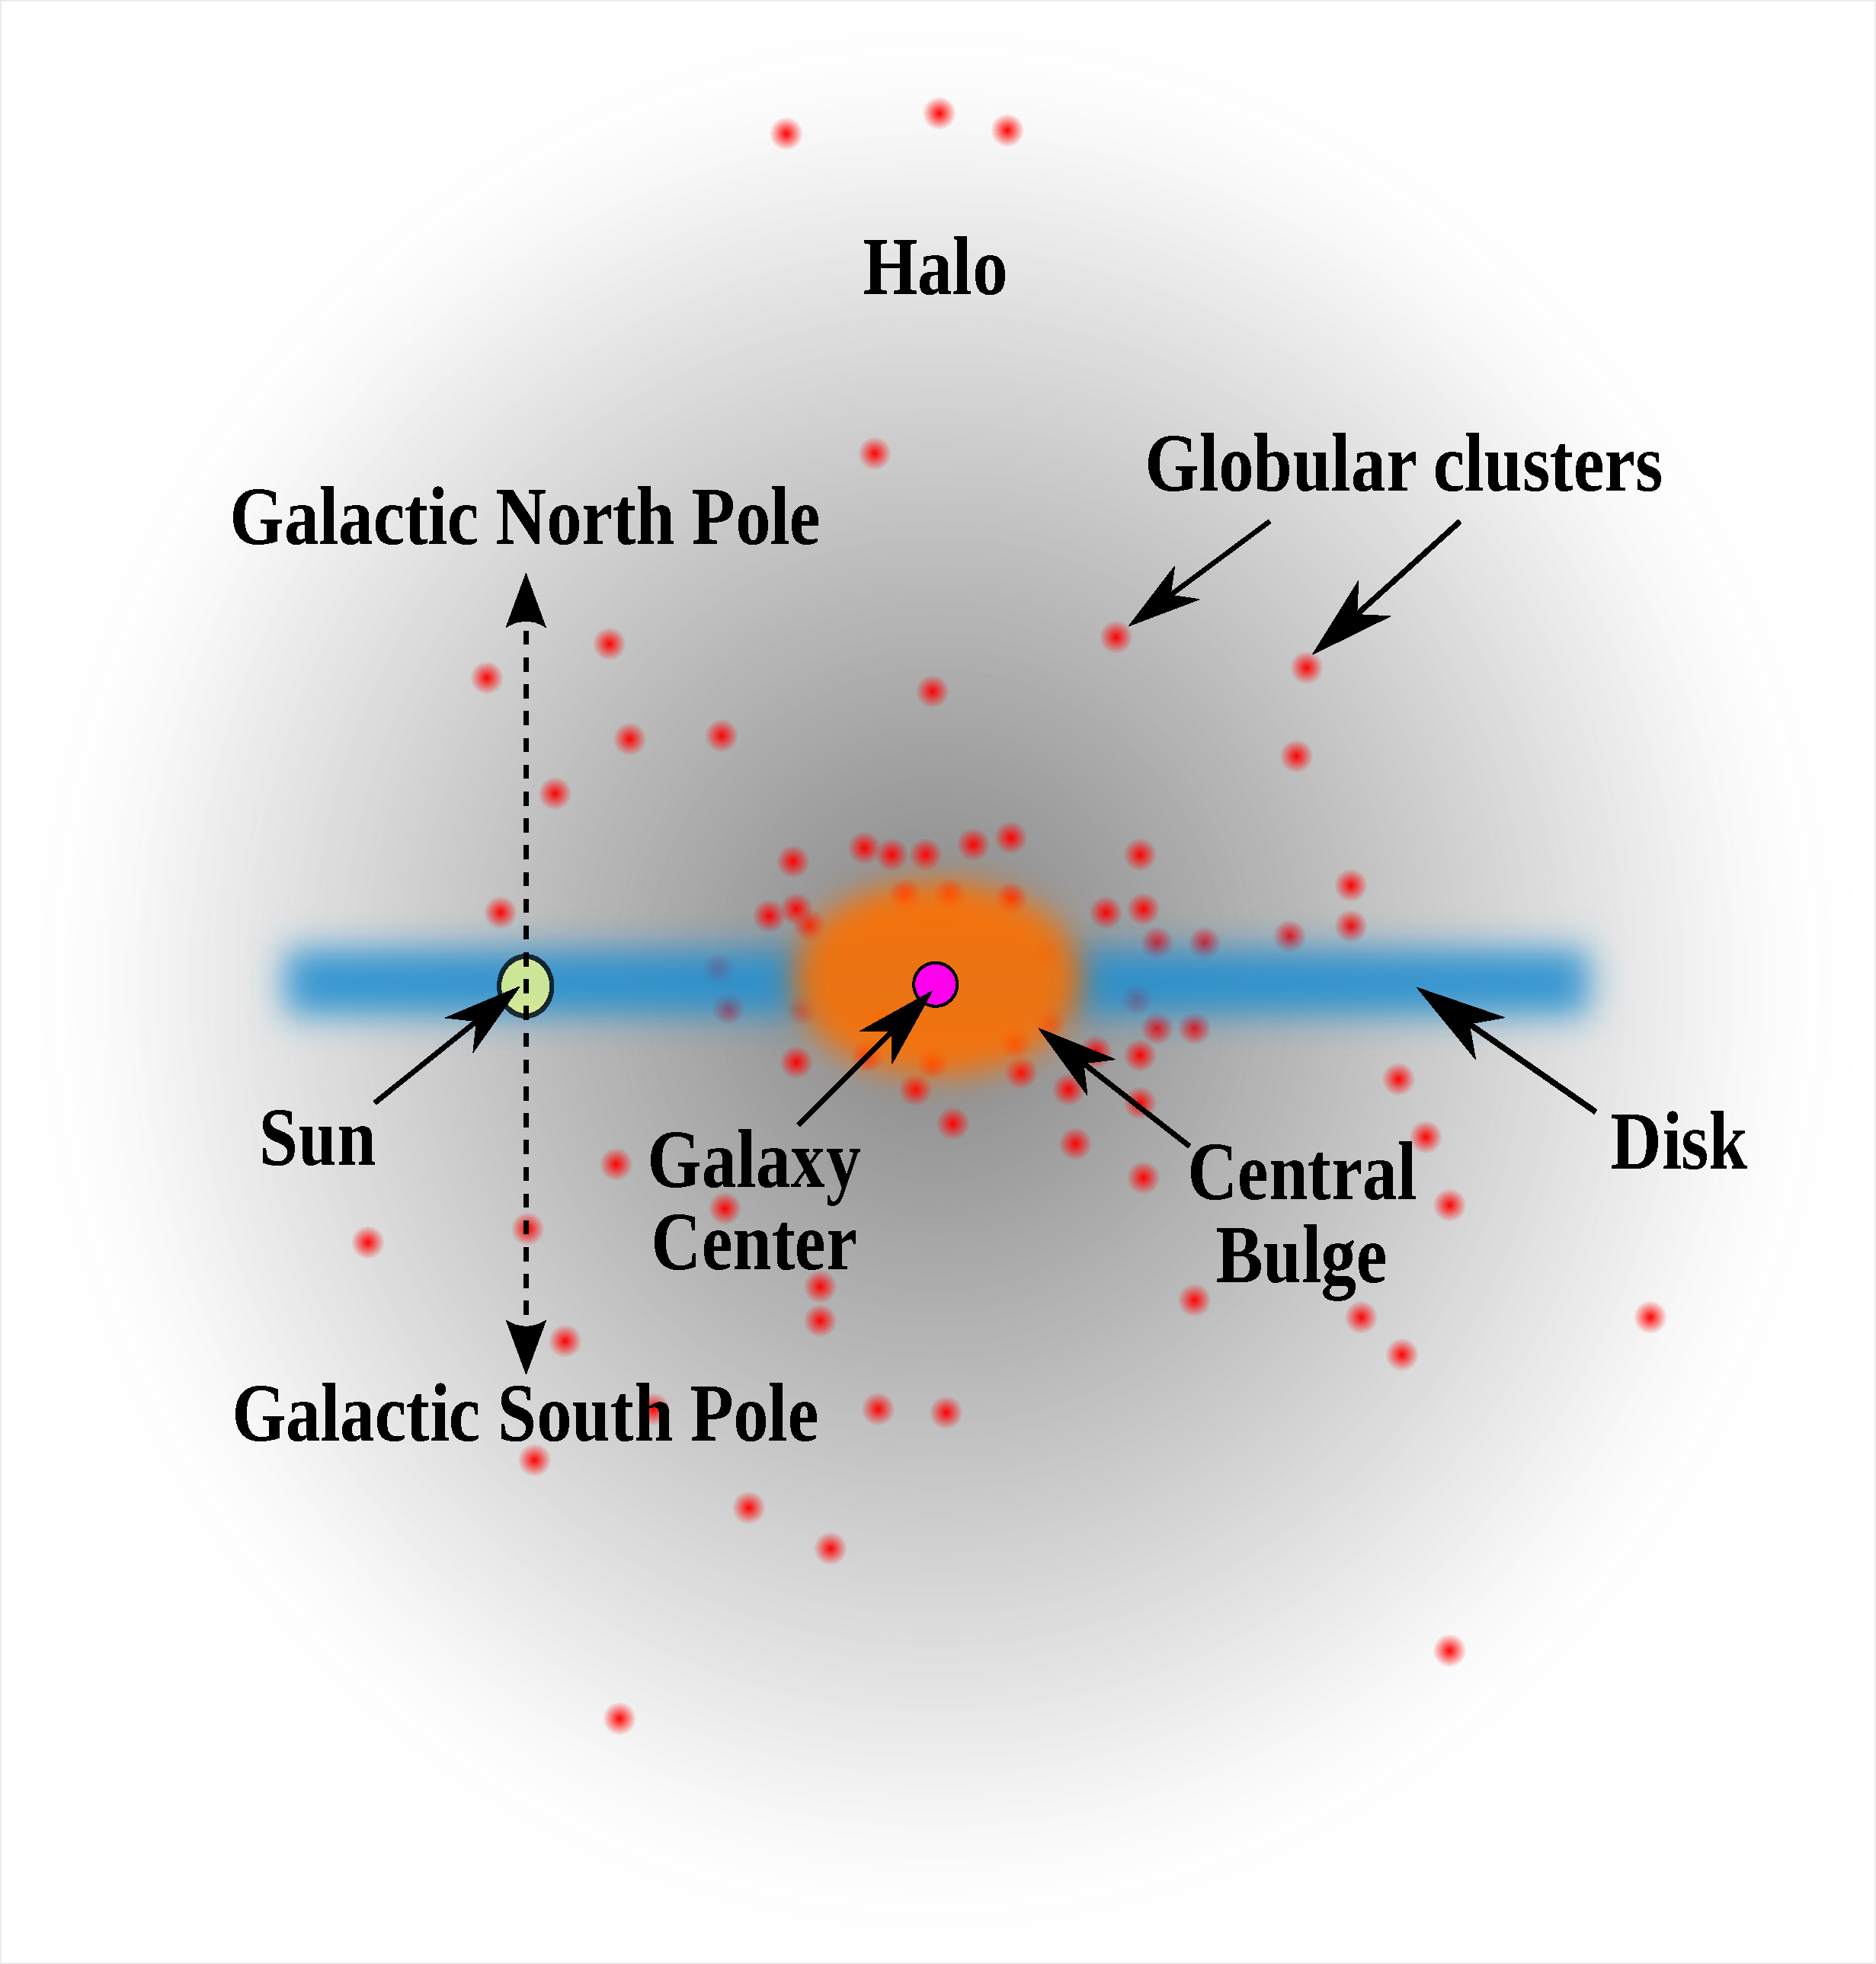
\includegraphics[width=\textwidth]{graphics/solar_system_abundances/milky_way_profile_wiki}
    \end{subfigure}
    \begin{subfigure}{0.5\textwidth}
        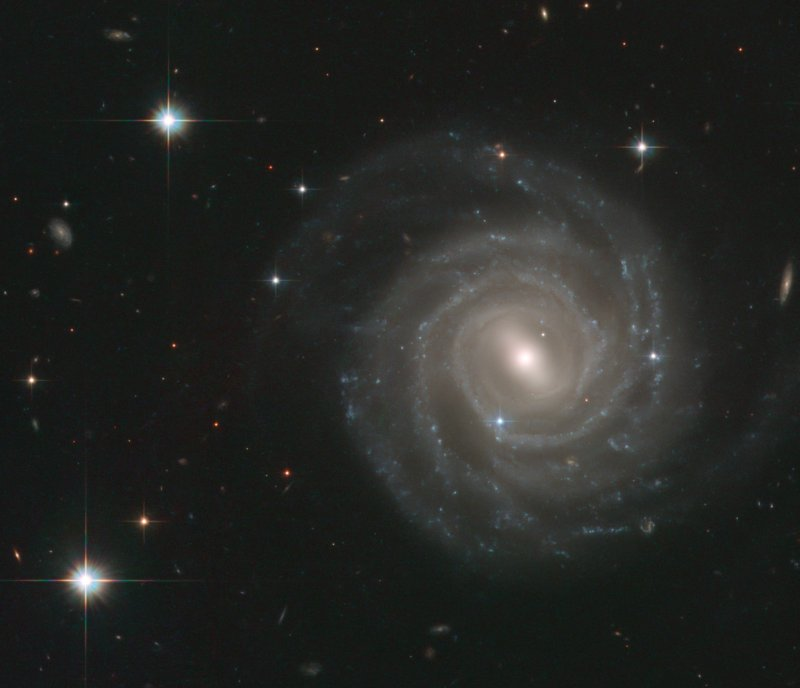
\includegraphics[width=\textwidth]{graphics/solar_system_abundances/UGC_12158}
    \end{subfigure}
    \caption{Left: Profile of the Milky Way with the current position of the Solar System indicated. Edited from \href{https://en.wikipedia.org/wiki/Milky_Way}{Wikipedia}. Right: Galaxy UGC 12158, which is thought to have a similar spiral structure as the Milky Way. Credit: ESA/Hubble \& NASA}
    \label{fig:milky_way_profile_wiki}
\end{figure}
In order to put the Solar System abundances in perspective to the galaxy, Figure~\ref{fig:milky_way_profile_wiki} shows a schematic of the Milky Way (left). The galactic center, which is likely a black hole, is surrounded by an area called the bulge. The disk of the Milky Way has a spiral structure. An analogue galaxy with a similar structure is UGC 12158, shown on the right in Figure~\ref{fig:milky_way_profile_wiki}. The densest regions of the Milky Way are close to the center (e.g., the bulge) while less dense areas are further out (e.g., the disk). The Solar System is located in the disk and about two-thirds out from the center in one of the spiral arms called the Orion-Cygnus arm. Disk and bulge are both surrounded by a low-density halo. This halo also contains globular clusters, which are gravitationally bound aggregations of stars. These clusters tend to be very old and are thus made of material that formed early on in the history of the Milky Way.

This chapter discusses the composition of the Solar System 4.567\,Ga ago (the initial Solar System abundances) and today (abundances in the solar photosphere). While we can observe stars and determine their composition via spectroscopy, the Solar System is unique since we have meteorites available that represent unaltered solar nebula material. This material is especially useful since it can be studied in the laboratory using mass spectrometry techniques. 

\codebox{Initial Solar System abundances in python}{can easily be handled with the \href{https://github.com/galactic-forensics/iniabu}{\texttt{iniabu}} package. This package can be used make various databases of Solar System abundances available for interaction and is used here to create abundance plots using \href{https://www.matplotlib.org}{\texttt{matplotlib}}. Full disclosure: I am the author of the package and am thus surely biased.}


\section{Definitions and Notations}

\subsection{Terminology}

\textbf{Elemental concentrations and abundances} are two terms that are often used interchangeably and their meaning, unfortunately, is often ambiguous. Let us for example look at a form of uranium oxide named \href{https://en.wikipedia.org/wiki/Yellowcake}{yellowcake}. The chemical formula for a common form of yellowcake is U$_3$O$_8$, i.e., the smallest unit consists of three uranium atoms and eight oxygen atoms. Expressing the stoichiometric elemental abundance of oxygen in yellowcake, i.e., the abundance by number of atoms, we would say that the oxygen abundance of yellowcake is $8 / (8+3) = 0.73$. Alternatively and often (but not exclusively referred to as the concentration) we could determine the oxygen concentration by mass. Uranium (mean mass: $\bar{m}_{\tn{U}} = 237.3$\,u) is significantly heavier than oxygen (mean mass: $\bar{m}_{\tn{O}} = 16.0$\,u). The mean mass here is the mass averaged over all isotopes of the specific element. The average concentration of oxygen in yellowcake, by mass, can then be determined as:
\begin{equation}
    [{\tn{O}}] = \frac{8 \bar{m}_{\tn{O}}}{8 \bar{m}_{\tn{O}} + 3 \bar{m}_{\tn{U}}} = 0.15
\end{equation}
Note that when solar abundances with respect to meteorites, the stoichiometric / number abundances are generally used. Astronomers and astrophysicists on the other hand often report mass fractions (see below).

\textbf{Solar (elemental) mass fractions} are commonly used in astronomy. For astronomers, the universe consists, to first order, of three elements, namely hydrogen ($X$), helium ($Y$), and metals ($Z$), which are all elements heavier than helium. This might sound strange since it implies that the air we breathe (78\% nitrogen, 21\% oxygen) consists of metals in the astronomical sense, however makes some sense when looking, e.g., at the composition of the Sun. The Sun's composition in this notation is $X=0.7389$, $Y=0.2463$, and $Z=0.0148$. These mass fractions are always given by weight.

\textbf{Solar System initial abundances}, often referred to as Solar System abundances, describe the original composition of the Solar System 4.567\,Ga ago. To determine this composition, measurements of, e.g., meteorites must be decay corrected for radioactive nuclides and their products.

\textbf{Solar photospheric abundances} on the other hand refer to the present-day composition of the Sun. There are further important differences between initial and present-day abundances that are discussed in the subsequent sections.

\infobox{Radioactive decay}{Unstable atomic nuclei undergo radioactive decay to so-called daughter nuclei. For example, \ex{26}Al is an unstable isotope and decays to the stable \ex{26}Mg. Its half-life ($t_{1/2}$), which is the time after which only half the initial material is left, is $7.17\times10^{5}$\,a. Radioactive decay is an exponential process. Instead of the half-life the decay constant $\lambda = \ln{2} / t_{1/2}$ is often referred to. Radioactive decay can be calculated as:
\begin{equation}
    N(t) = N_0 \exp{(-\lambda t)} \label{eqn:radioactive_decay}
\end{equation}
Here, $N_0$ is the amount of radioactive material available at $t=0$ and $N(t)$ is the amount of material after time $t$ has elapsed.}

\subsection{Scales}

As with definitions, several different scales are used. Here we define the three most commonly used ones. \textbf{Meteoritic abundances} are generally normalized to the number of silicon atoms, which is set to be equal to $N_\tn{Si} = 10^{6}$. These abundances scale linearly.

\textbf{Spectroscopic abundances}, often used in astronomy, are frequently given with respect to hydrogen, the most abundant element in the universe. These abundances are usually reported as logarithmic abundances and the abundance of hydrogen is defined to be equal to 12. For example, the Solar System initial abundance of silicon in this logarithmic unit can be calculated as:
\begin{equation}
    A(\tn{Si}) = \log_{10} \left( \frac{N_\tn{Si}}{N_\tn{H}}\right) + 12 = 7.59
\end{equation}
Here, $N_\tn{Si}$ and $N_\tn{H}$ are the number abundances of silicon and hydrogen, respectively.

Finally, \textbf{mass fractions} are also frequently used in astronomy and astrophysics. The mass fraction of an element or isotope $x_i$ with number abundance $N_i$ and mass $m_i$ can be calculated as:
\begin{equation}
    x_i = \frac{N_i m_i}{\sum_j N_j m_j}
\end{equation}
Here, the sum over $j$ adds up all elements or isotopes. If we were thus to sum up all mass fractions, we would get $\sum_j x_j = 1$.


\subsection{Comparing measurements}


In astronomy, chemical abundance ratios are generally expressed in ``bracket''-notation. These chemical abundance ratios are then usually regarded with respect to a standard, which generally is the Sun. For example, to express the iron content of a given star in comparison to the Sun one would calculate:
\begin{equation}
    [\tn{Fe}/\tn{H}] = \log_{10} \left( \frac{N_\tn{Fe}}{N_\tn{H}}\right)_\tn{star} - \log_{10} \left( \frac{N_\tn{Fe}}{N_\tn{H}}\right)_\odot
\end{equation}
Here, $N_x$ represents the number abundance of a given element $x$. The symbol $\odot$ is generally used for the Sun. Using this formulation, observations with higher iron content than the Sun would result in a positive number, and vice verse. While the [Fe/H] number is unitless, differences in this notation are commonly referred to as \ac{dex}. A star with a $0.3$\,dex enhancement in [Fe/H] would thus have twice as much iron than the Sun when normalized to hydrogen.




\section{The Sun}\label{sec:solar_system_abundances:the_sun}

The Sun is the central body of the Solar System and contains with a mass of $\sim2\times10^{30}$\,kg about 99.86\% of the total mass in the Solar System. The total luminosity of the Sun is $3.8\times10^{26}$\,W and it's orbited by the Earth at a mean distance of $\sim1.5\times10^{8}$\,km, which is equal to 1 \ac{au}. The total solar irradiance at Earth is thus around 1.3\,kW/m$^{2}$.

\begin{figure}[tb]
    \centering
    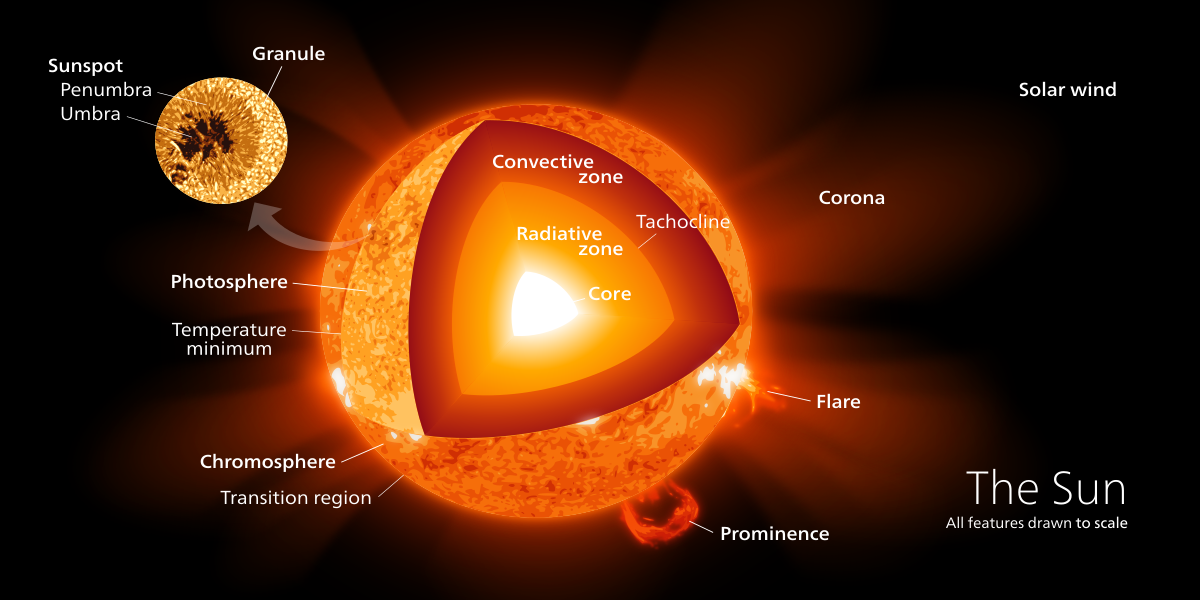
\includegraphics[width=0.8\textwidth]{graphics/solar_system_abundances/sun_structure}
    \caption{The structure of the Sun. Credit: Kelvinsong via \href{https://en.wikipedia.org/wiki/Sun}{Wikipedia}.}
    \label{fig:Sun_structure}
\end{figure}
Since the Sun contains the majority of the Solar System's mass, it is reasonable to assume that this celestial body also represents well the Solar System's composition. Figure~\ref{fig:Sun_structure} shows an artistic rendering of the structure of the Sun. The Sun's core extends to about a quarter of its radius and is the main nuclear engine that fuses hydrogen to helium at a temperature of around $16\times10^{6}$\,K.\footnote{Temperatures in astrophysics are often written as $T_x = y$. In this case, the actual temperature would be $y\times10^{x}$\,K. For the core of the Sun we could write the temperature thus as $T_{10} = 1.6$.} The solar core is not convectively connected to the outer layers, thus energy is mainly transported by radiative transfer. The photosphere, which is the visible part of the Sun, is at a temperature of around $5800$\,K. The atmosphere of the Sun has a minimum temperature of around 4100\,K about 500\,km above the photosphere. It consists of the chromosphere which lays above the photosphere and the solar corona that extends from the chromosphere out into space. At higher altitudes the temperature of the corona increases and reaches temperatures in excess of $10^6$\,K. How such high temperatures can be reached in the solar corona is still unclear.

\morebox{Wien's displacement law}{states that the radiation curve of a black-body has it's peak at different wavelengths depending on the temperature. For a given temperature, the peak wavelength can be calculated as:
\begin{equation}
    \lambda_\tn{max} = \frac{b}{T}
\end{equation}
Here, $T$ is the temperature in kelvin and $b = 2.898 \times 10^{-3}$ m$\cdot$K. Plugging in the photosphere temperature, we can calculate a peak wavelength at 500\,nm, which is the color green in the visible part of the electromagnetic spectrum.}


\subsection{Spectroscopy and Absorption Spectra}

\begin{figure}[tb]
    \centering
    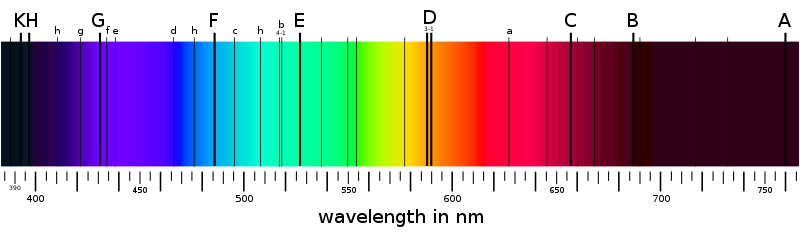
\includegraphics[width=0.8\textwidth]{graphics/solar_system_abundances/fraunhofer_lines_800px}
    \caption{The solar spectrum broken up into its components. Credit: \href{https://en.wikipedia.org/wiki/Fraunhofer_lines}{Wikipedia}.}
    \label{fig:fraunhofer_lines}
\end{figure}
In order to determine the composition of the Sun from the electromagnetic spectrum it radiates, astronomers use a technique called stellar spectroscopy. Using a prism or grating the light from the Sun is dispersed into its individual colors. Figure~\ref{fig:fraunhofer_lines} shows the electromagnetic spectrum of the Sun between 380\,nm and 710\,nm. Clearly visible are dark spectral absorption lines, so-called Fraunhofer lines named after Joseph von Fraunhofer who discovered, studied, and described them in 1814.

These absorption lines are fingerprints of the Sun's elemental composition. The dark lines form since photons coming out of the Sun are absorbed in the photosphere by atoms. The absorbed photons are subsequently re-emitted, however, this re-emission is not directed. Thus, the area of the spectrum that the original photon was absorbed in appears darker. For example, the double lines labeled ``D'' in Figure~\ref{fig:fraunhofer_lines} are a feature of the sodium absorption lines.


\subsection{Stellar Abundances} \label{sec:solar_abundances:sun:stellar_abundances}

In order to interpret the Fraunhofer lines observed from the Sun with respect to its elemental composition, many physical parameters and models must be known. Here we give a brief overview of these modeling efforts. Further details can be found in two great reviews on determining the Sun's elemental composition by \citet{asplund09} and \citet{allende-prieto16}.

To determine the composition of the Sun two closely related conditions must be understood: (1) line formation and (2) the stellar atmosphere. These two fields include physics from several disciplines, namely fluid dynamics, statistical mechanics, and thermodynamics. To understand line formation the atomic parameters and stellar conditions, such as the opacity, need to be known. To model stellar atmospheres on the other hand we need to know the energy radiated through the atmosphere, the surface gravity, and the chemical composition. Note that the chemical composition is on one hand what we would like to determine from these observations, however it is also an integral part of the stellar atmospheric model. The chemical composition has thus to be determined in an iterative process. For a given set of interest, especially the amount of energy radiated through it, its surface gravity, and its chemical composition. Note that the chemical composition, which is what we would like to find, must be known in order to model the stellar atmosphere. Determining the composition of the Sun from observations is thus an iterative process. For a given model atmosphere and determined atomic and molecular lines and continuum opacities, so-called spectra synthesis codes can be used to predict the spectrum of the model star with all its absorption lines. These spectra are then compared to observations. If different, the parameters, especially the chemical composition is updated with better values and the models are run again. The chemical composition of the star is found when model and observations agree.




\subsubsection{Photospheric Abundances}

The solar photosphere (see Figure~\ref{fig:Sun_structure}) is the part of the Sun that we can actually see. Spectroscopy of the photosphere is thus generally used to model the solar abundances. With a temperature between 4500\,K and 6000\,K and an effective temperature of around 5800\,K no molecules can form in the photosphere and thus only atoms are expected to contribute to its absorption lines. Furthermore, the densities of the chromosphere and corona above the photosphere are so low that they do not influence the absorption lines observed from the photosphere.

The present-day solar photosphere composition is slightly different from the initial Solar System abundance, i.e., the abundance that is representative of the homogeneous solar nebula. One difference of course is for radioactive nuclides that have decayed over the last 4.567\,Ga since the beginning of the Solar System. Furthermore, thermal diffusion, gravitational settling, and radiative acceleration -- the three of which are often collectively referred to as diffusion -- also changed the photospheric composition over the past 4.567\,Ga. Corrections for these effects must thus be applied before comparing Solar System initial abundances, as e.g., measured in meteorites (see Section~\ref{sec:sol_abu_meteorites}) with photospheric measurements.

\subsubsection{Chromosphere \& Corona Observations}

The chromosphere and corona are the solar layers right above the photosphere. These layers are too thin for us to directly observe and can generally only be seen during a total solar eclipse. Since there is no homogeneous background irradiation for the chromosphere and corona in these cases, absorption spectra cannot be measured. Thus, the elemental composition of the solar atmosphere is determined by measuring emission spectra. Excited atoms fall back to their ground states at discreet energies. Such emission lines will show up as bright instead of dark lines when analyzed in a spectrograph. 

Temperatures as low as 4100K have been measured in the chromosphere. This allows for the existence of simple molecules, which complicates the determination of the spectral abundances since many more atomic transitions are suddenly available. Furthermore, the chromosphere has a fairly large temperature gradient which also complicates the models. 

Coronal abundances are difficult to determine. The extremely high temperatures of the coronal make it difficult to determine radiative transitions in the laboratory. A large part of the coronal emission lines are furthermore in the \ac{uv} and \ac{euv}, thus can not be detected from Earth due to the atmosphere. Spacecrafts such as \ac{soho} have been used to determine the elemental composition of the solar corona.



\subsubsection{Solar Wind \label{sec:solar_abus:solar_wind}}

\begin{figure}[bt]
    \begin{subfigure}{0.470209674\textwidth}
        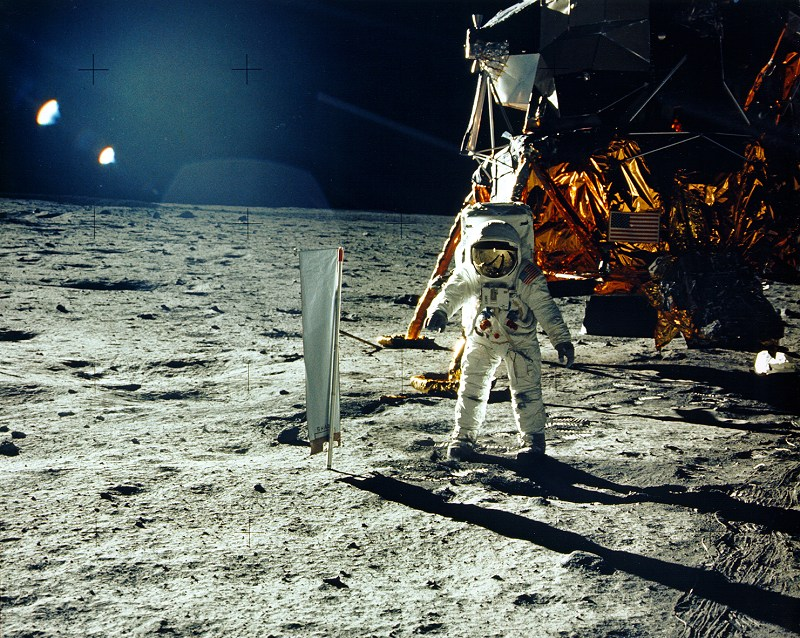
\includegraphics[width=\textwidth]{graphics/solar_system_abundances/apollo11_aldrin_solar_sail}
        \caption{Buzz Aldrin standing next to the solar sail during the Apollo 11 mission.}
        \label{fig:solar_wind_catcher_experiments:solar_sail}
    \end{subfigure}
    \begin{subfigure}{0.529790326\textwidth}
        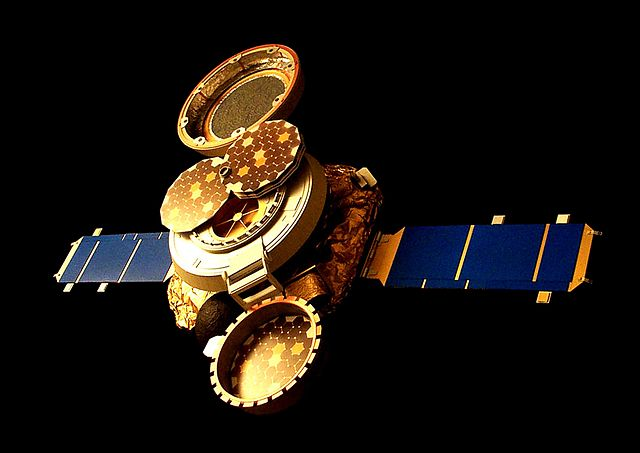
\includegraphics[width=\textwidth]{graphics/solar_system_abundances/genesis_spacecraft}
        \caption{Artist conception of the Genesis spacecraft with unfolded collectors.}
        \label{fig:solar_wind_catcher_experiments:genesis}
    \end{subfigure}
    \caption{The two types of solar wind catcher experiments that have been used to determine the composition of the Sun. Credit: NASA}
    \label{fig:solar_wind_catcher_experiments}
\end{figure}

Mass ejections such as prominences and flares (see Figure~\ref{fig:Sun_structure}) are the origin of the solar wind that penetrates the whole Solar System. The interaction of the solar wind with the Earth's magnetic field can, e.g., be seen as aurorae (borealis and australis), also known as the northern and southern lights. The solar wind consists to 98\% of protons (charged hydrogen particles). The other 2\% is mainly charged helium nuclei and a minute amount of heavier particles. This however means that the solar wind does carry some part of the Sun's composition out through the solar system.

While the solar wind cannot be measured on Earth, bodies without an atmosphere such as the Moon are constantly struck by solar wind. During the Apollo missions to the Moon, astronauts carried a solar sail, which was aluminum foil mounted on a pole in order to capture solar wind during their stay on the Moon. Figure~\ref{fig:solar_wind_catcher_experiments:solar_sail} shows Apollo 11 astronaut Buzz Aldrin standing next to the solar sail. While valuable measurements were done using solar sails flown on Apollo missions, the total exposure time of the aluminum foil was very limited, i.e., only up to a few days each. Thus, only little material was captured which resulted in significant analytical uncertainties when measuring the captured content.

In 2001, NASA launched the Genesis spacecraft which was parked on a Lagrange point L$_1$.\footnote{For more information, see \url{https://en.wikipedia.org/wiki/Lagrangian_point}} L$_1$ is a gravitationally semi-stable place in space in between the Sun and the Earth. Genesis exposed its collectors (Figure~\ref{fig:solar_wind_catcher_experiments:genesis}) to the solar wind for a total of 850\,d before returning to Earth. In order to avoid any contamination with terrestrial material, NASA's plan was for Genesis to re-enter the Earth's atmosphere, deploy its drogue parachute, and then capture the capsule mid-air using a helicopter with a long hook. The deployment mechanism for the parachute was connected to an accelerometer, which was unfortunately built backwards into the spacecraft. This resulted in the accelerometer measuring the acceleration with the wrong sign, thus never triggering the software to release the parachute. Needless to say that the ``landing'' of Genesis took place at a terminal velocity of around 86\,m\,s$^{-1}$ (190\,mph). This broke open the collector container and all collectors were significantly contaminated with material from the Utah dessert. Nevertheless, all main objectives of Genesis could still be achieved by meticulously cleaning and puzzling the collector array back together, a process that took several years.


\section{Meteorites}\label{sec:sol_abu_meteorites}

Meteorites are rocks that originated in the Solar System and fell to Earth as meteors. They are either finds, meaning that they were found during searches, or falls, meaning that they were found after observing the meteor in the sky. Meteorites could have previously been part of another planet, e.g., Mars, part of the Moon, or, most often, part of an asteroid. Thousands of these rocks have been analyzed, and they are generally classified into various different groups. The two major groups these rocks belong to relate them to their origin; they were either part of a differentiated or an undifferentiated parent body. A differentiated Solar System body has at some point in its history gotten hot enough in order to be completely or partially molten. This separated the metal-loving (siderophile) from the silicate loving (lithophile) elements. The Earth for example is a differentiated body with an iron, nickel core at the center and a silicate mantel around it. Meteorites from undifferentiated bodies, called chondrites, still contain the metal and silicate in the same phases, i.e., they have never gotten hot enough to differentiate. 

In order to determine the initial Solar System composition by analyzing meteorites, samples that have never been altered throughout its history are of special interest. These meteorites are called primitive. The most primitive subgroup of the chondrites are the carbonaceous chondrites, which have generally not even been heated enough in order to destroy the mineral phases that originally condensed from the solar nebula.

Alterations different from heat, e.g., chemical alterations, can also influence the composition and thus primitiveness of a meteorite. Meteorites that have been the least altered with respect to their chemical and isotopic composition are carbonaceous chondrites that are similar to the Ivuna meteorite, which is the type specimen for this group. The name of this chondrite group is thus abbreviated CI chondrites. The Orgueil meteorite, a CI chondrite, represents the best studied sample for the Solar System initial abundance. This rock fell on May 14, 1864 just after 8pm local time near Orgueil, a town in southern France. Samples were recovered immediately, totaling 14\,kg of material. Meteorite falls have the advantage that they did not spend any significant amounts of time exposed to the weather on Earth, thus they do not show any terrestrial alteration either. 

To determine the composition of meteorites, their material is usually homogenized and then analyzed using a mass spectrometery. Depending on the element of interest sample material is atomized and ionized. These ions are then separated by mass-over-charge in a mass analyzer. This allows for precise determination of their elemental and isotopic composition.

\morebox{Stardust}{Some primitive meteorites contain micrometer sized grains that in fact did not form in the Solar System at all but rather represent bona-fide stardust grains. These stardust grains formed in the outflow of dying stars, were transported through the \ac{ism}, and then incorportated into meteorite parent bodies during their formation. We will discuss stardust grains in more detail later since these samples allow us to directly probe the processes in which elements are created.}



\section{The Composition of the Solar System}

While CI chondrites seem to be primitive Solar System objects, their total mass is represents only a tiny fraction of the total mass of the Solar System. Photosphere observations on the other hand are associated with larger measurement uncertainties and require modeling of the physical processes underlying the formation of absorption spectra. The question thus arises on how the composition of the Solar System can best be determined.

\subsection{Comparing CI chondrites and the Photosphere}

\begin{figure}[bt] \centering
    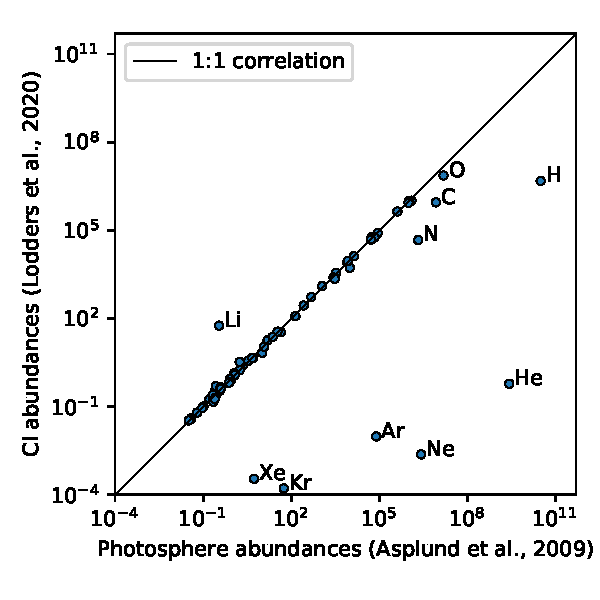
\includegraphics[width=0.5\textwidth]{graphics/solar_system_abundances/solar_photosphere_ci_abundances_correlation}
    \caption{Comparison of solar photosphere measurements \citep{asplund09} and the composition of CI meteorites \citep{lodders20}. Elements that do not lie close to the 1:1 correlation line are labeled.}
    \label{fig:solar_photosphere_ci_comparison}
\end{figure}
Figure~\ref{fig:solar_photosphere_ci_comparison} shows the comparison of the photosphere measurements reported in \citet{asplund09} with the CI chondrite measurements reported in \citet{lodders20}. Most elements lie perfectly on the 1:1 correlation indicated in black in the figure, which spans a total of around 12 orders of magnitude. However, there are some very notable deviations that require further discussion.

\paragraph{Lithium} is the only element that is more abundant in CI chondrites than in the Sun. In the Sun, lithium diffuses effectively. Since it is destroyed during the nuclear reactions taking place in the stellar core, the overall abundance of lithium is expected to be depleted when compared to the bulk Solar System.

\paragraph{The noble gases} helium, neon, argon, krypton, and xenon are all very volatile and are thus heavily depleted in meteorites, i.e., they never effectively condensed into the rocky material when meteorite parent bodies formed. The bulk Solar System helium abundance can fortunately be derived from helioseismology via observations of the Sun and is not highly model dependent. Various techniques have been used to determine the composition of the other noble gases. One of the most accurate methods to-date is the analysis of solar wind in the Genesis collectors, see page~\pageref{sec:solar_abus:solar_wind}.

\paragraph{Hydrogen} is also a highly volatile element and thus does not effectively condense into meteorite parent bodies. Hydrogen thus needs to be measured in the Sun by model comparison. The hydrogen mass is insensitive to the Z/X composition of the Sun, which results in an accurate determination of the hydrogen mass fraction X.

\paragraph{Carbon, nitrogen, and oxygen} are prominent atoms that form volatile molecules, e.g., CO, CO$_2$, N$_2$, and O$_2$. Thus, these elements are expected to be depleted in rocky materials. While these elements can all be measured in the solar photosphere, model improvements resulted in significant changes over time in their abundances.

\subsection{Solar System Elemental Abundances}

\begin{figure}[bt] \centering
    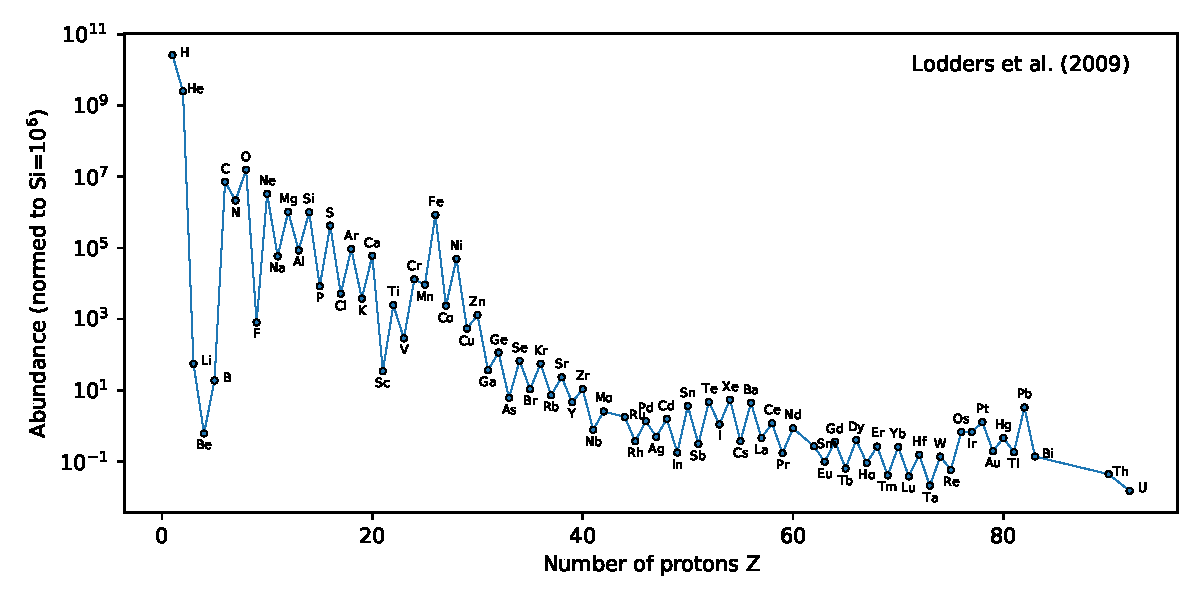
\includegraphics[width=\textwidth]{graphics/solar_system_abundances/solar_system_abundances}
    \caption{Solar System initial abundances for all elements \citep{lodders09}.}
    \label{fig:solar_system_abundances}
\end{figure}
Figure~\ref{fig:solar_system_abundances} shows the elemental abundances of the solar nebula. Clearly, hydrogen and helium are the most abundant elements. Furthermore, we can see a clear peak around carbon, oxygen, and neon. These elements are made in most stars and thus reach such high abundances. There is also a clear peak at the iron isotopic composition. This is due to the fact that in this region, the binding energy per nucleon is the highest across all elements. That means that energy can be gained by fusing nuclides together up to iron. Past iron this does not happen anymore, thus the abundances of all heavier nuclides drop significantly.

Another striking feature of the abundance curve in Figure~\ref{fig:solar_system_abundances} is the clear zigzag pattern. This pattern is due to the fact that even nuclei, i.e., nuclei with an even number of nucleons (protons and neutrons), have a higher binding energy than odd nuclei and are thus more stable. 


\subsection{Solar System Isotopic Abundances}

So far we have mostly discussed the abundance of the elements in the Solar System. Just as important is the abundance of the isotopes, which can be derived from CI chondrites with high precision. Atomic line differences of individual isotopes are generally too small in order to derive useful isotopic abundances from solar observations. Let us briefly discuss the origin of a few important isotopes cannot easily be derived from CI chondrites.

\paragraph{Deuterium and \ex{3}He} are both highly volatile, thus cannot be measured in CI chondrites, and have been significantly changed in the Sun. In its early stage the Sun underwent deuterium burning, essentially leaving it deuterium free at this point. This burning also produced \ex{3}He and thus changed its abundance in the Sun. The exact D/H ratio in the Solar System is still an active matter of research. Good analogues to determine this ratio are the atmosphere of Jupiter which consists mainly of the gaseous material that the solar nebula was made of, and in comets. Certain, so-called Kuiper-belt comets formed far out in the Solar System beyond the snow-line, which is the area of the solar nebula beyond which water only appears in solid form. These comets thus trapped the original D/H composition. For the early Solar System \ex{3}He/\ex{4}He ratio, the value for Jupiter's atmosphere is generally adopted.

\paragraph{Carbon, nitrogen, and oxygen} are all very volatile. While the carbon isotopic composition in the Solar System is not very variable across different types of meteorites, the nitrogen and oxygen isotopic composition vary widely. To measure these isotopes in solar wind was one of the main objectives of the Genesis mission. After significant cleaning of these collectors, the solar oxygen and nitrogen isotopic composition have finally been determined by \citet{mckeegan11} and \citet{marty11}, respectively.

\paragraph{Noble gases} are also volatile. As discussed before, their elemental and isotopic abundances were determined using the solar wind collectors on board the Genesis spacecraft. A detailed review of this work can be found in \citet{heber09}.



\subsection{Preview on the Origin of Elements and Isotopes}

So far we have only briefly discussed the major features visible in the Solar System abundance pattern (Figure~\ref{fig:solar_system_abundances}). We will look into a lot more details on how individual elements and groups formed later on. The production of elements and their isotopes takes place in a process called nucleosynthesis. A brief overview of these processes is given below.

All hdrogen and helium in universe formed right after the Big Bang in a process called \acl{bbn}. The majority of all heavier elements were subsequently formed in stars. Elements up to the iron peak formed mainly in massive stars by nuclear fusion reactions. As discussed before, the binding energy per nucleon is the highest at iron and thus fusion reactions beyond this region are not energetically favorable. Thus, other processes must take over. 

Most isotopes beyond iron are formed by neutron-capture reactions. Since neutrons are not electrically charged, they do not see the Coulomb barrier of a positively charged nucleus and can thus be more effectively added to it. Neutron addition takes place until the nucleus becomes unstable. Unstable, neutron-rich nuclei decay generally via $\beta^{-}$-decay to the next stable isobar, which has one proton more and one neutron less. Proton-rich nuclei, e.g., \ex{92}Mo, cannot form by neutron capture and various processes and locations for their formation are actively being discussed in the astrophysics community.

About half the elements beyond iron formed in the so called \ac{sproc}, in which the $\beta^{-}$ decay to the stable isobar generally happens faster than another neutron can be captured. This way however, only elements up to bismuth can be made. Heavier elements, e.g., actinides such as thorium and uranium, cannot be formed in the \ac{sproc}. Rapid capture of neutrons, the so-called \ac{rproc}, must thus be invoked to explain their existence.



\section{Other Stars}

While we have Solar System samples, i.e., CI chondrites, to determine the composition of the solar nebula and thus the Sun precisely, representative rocks of other stars are not available in the Solar System. However, the light of other star still reaches us, i.e., we can see their photosphere and apply the same spectroscopic techniques to determine their elemental composition. 

As discussed in Section~\ref{sec:solar_abundances:sun:stellar_abundances}, to determine the abundances of observed other stars, the stellar atmosphere must be modeled. For this, the size and mass of the star must be known, which is not always simple to determine from observations. Recent massive surveys such as the Sloan Digital Sky Survey\footnote{\url{https://www.sdss.org/}} and the Gaia mission\footnote{\url{https://sci.esa.int/web/gaia/}} have made it possible to determine the elemental composition of many more stars. An overview of existing database can, e.g., be found in \citet{allende-prieto16}. It turns out that the solar neighborhood is a diverse place \citep[see, e.g.,][]{bensby14} and still leaves us for the time being with many open question on the origin of its elements and isotopes.

\section{Reading}

A great reading to further dive into the topic of solar abundances is the recent review by \citet{lodders20}.\footnote{At the time of this writing, the download of the document as a \ac{pdfdoc} file did not succeed. You can also find this article on \href{https://arxiv.org/abs/1912.00844}{ArXiV}.} Some questions and points of discussions for this paper are:
\begin{itemize}
    \item Why are meteoritic measurements normalized to a silicon abundance of $10^6$ while astronomical observations are generally given in \ac{dex} noramlized such that the abundance of hydrogen is equal to 12?
    \item Why can elemental abundances with much higher precision in CI chondrites than in the Sun's photosphere?
    \item Why does aqueous alteration not affect the chemical composition of CI chondrites?
    \item Explain from a nuclear physics point of view why there is no deuterium in the Sun.
    \item Why is it so difficult to determine certain elemental and isotopic abundances, e.g., noble gases and the D/H ratio of the Solar System?
    \item What are the difficulties that one encounters when analyzing meteorites by mass spectrometry?
    \item Why can carbon, oxygen, and nitrogen not be determined when analyzing meteorites?
\end{itemize}
%!TEX root = origin_elements_lecture_notes.tex

\chapter{Big Bang Nucleosynthesis}

In order to understand primordial / \acf{bbn}, we need to first look at some fundamental observations that define cosmology. In addition, we also need to introduce the standard model of cosmology. Note that this is only a very brief introduction into a topic that could be a whole course by itself.

\section{Fundamental Cosmological Observations}

\subsection{Olbers' paradox}

One of the most fundamental observations that goes back to Kepler (1610), Halley (1721), de Cheseaux (1744), and is today known as Olbers' (1823) paradox is the fact that the night sky is dark. If one assumes an infinite, homogeneous space filled with stars, this space would appear infinitely bright to the observer on Earth. The apparent luminosity of a star can be described as
\begin{equation}\label{eqn:bbn:relative_luminosity}
    l = \frac{L}{4 \pi r^{2}} \propto r^{-2},
\end{equation}
where $L$ is the star's luminosity and $r$ its distance from Earth. Assuming a density of stars $n$, a spherical shell of thickness $dr$ at distance $r$ from Earth would contain
\begin{equation}
    dN = 4 \pi n r^2 dr \propto r^2
\end{equation}
stars. The total energy density of all stars for an observer can thus be calculated as
\begin{equation}\label{eqn:bbn:total_energy_density}
    \varepsilon_s = \int_0^{\infty} \frac{L}{4\pi r^2} dN = nL \int_{0}^{\infty} dr.
\end{equation}
In contrast to our experience this integral is divergent, thus the night sky should be infinitely bright. 

This paradox cannot be simply solved by assuming absorption of light in the interstellar medium, e.g., by dust. The energy from all stars would over time heat up this dust until it radiates as bright as the stars themselves. One factor that slightly helps is that stars will overlap with each other. You can picture this scenario however like standing in a dense forest where, as far as you can see, every line of sites terminates in a tree trunk. For the universe this would mean that every line of sight will terminate at the surface of a star. Stars cover each other, so the night sky would not seem infinitely bright but homogeneously about as bright as the Sun. This still does not agree with our experience.

The solution to the paradox lies in the fact that the universe is expanding. The wavelength of the light that arrives expands along with the universe and is thus shifted to the red (Doppler shift). The result is that the relative luminosity, as given in equation \eqref{eqn:bbn:relative_luminosity}, is in fact $l\propto r^{-3}$. Plugging this into equation~\eqref{eqn:bbn:relative_luminosity} results in the integral converging. In addition, there the universe has a horizon at distance
\begin{equation}
    R \simeq ct.
\end{equation}
Here, $c$ is the speed of light and $t$ the approximate age of the universe. The visible part of space and thus the energy density become finite.

\infobox{Doppler effect}{Let us assume that a source emits an electromagnetic wave with wavelength $\lambda_s$. An observer that moves with a velocity $\vec{v}$ with respect to that source will register a shifted frequency $\lambda_r$. For light, and considering special relativity, this effect will result in a blueshift if the observer moves towards the source and in a redshift if the observer moves away from the source. For two objects that move directly towards or away from each other, the relativistic Doppler shift for light can be written as
\begin{equation}\label{eqn:bbn:relativistic_doppler_shift}
    \lambda_r = \sqrt{\frac{1+\beta}{1-\beta}} \lambda_s,
\end{equation}
where $\beta = v/c$, i.e., the speed of the observer $v$ with respect to the speed of light $c$. Sources moving away from each other hereby have a postive velocity ($\beta > 0$), sources moving towards each other a negative one ($\beta < 0$).}

\subsection{Hubble's Law}

\begin{figure}[tb]
    \centering
    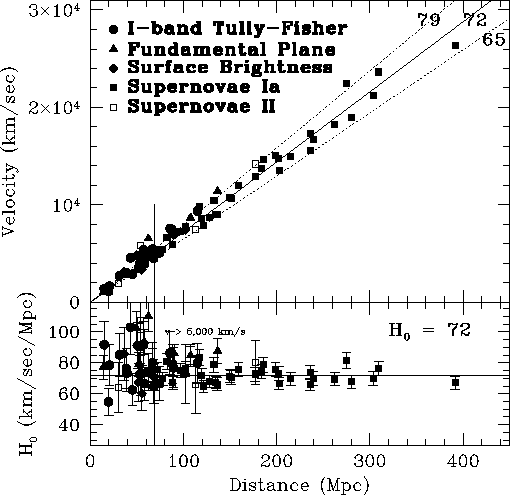
\includegraphics[width=0.5\textwidth]{graphics/bbn/hubble_diagram}
    \caption{Hubble diagram of velocity (top) and value of $H_0$ (bottom) as a function of distance. \cite{freedman01}, \copyright\ 2001 The American Astronomical Society.} 
    \label{fig:bbn:hubble_diagram}
\end{figure}
The expansion of the universe can in fact be observed. Figure~\ref{fig:bbn:hubble_diagram} shows the Hubble diagram for many observations, taken from \citet{freedman01}. The diagram on top shows the velocity of objects relative to Earth as a function of their distance. Using the Doppler shift one can see that the velocity, which is away from the observer in this case, is proportional to the redshift of the object. Here, the distance is given in megaparsec, where 1\,\ac{pc} is approximately 3.26 light years. The linear relationship between velocity and distance (R) can be written as
\begin{equation}
    \left(\frac{\dot{R}}{R}\right)_0 = H_0 = \mathrm{constant}.
\end{equation}
The subscript zero hereby describes the present-day value of the constant. The constant $H_0$ is commonly called the Hubble constant and its value is about $H_0 = 70\,\mathrm{km}\,\mathrm{s}^{-1}\,\mathrm{Mpc}^{-1}$. Note that the Hubble constant is given in units of one over seconds. The reciprocal value of the $H_0$ thus defines a time, the so-called Hubble time. If the expansion of the universe is never accelerated, its age could be determined as
\begin{equation}
    t_0 \leq \frac{1}{H_0} = 1.4 \times 10^{10}\,\mathrm{a}.
\end{equation}

The distance of a galaxy is often expressed by its redshift. Let $\lambda$ be the wavelength sent out from the galaxy in question and $\lambda_0$ the wavelength received today. The redshift $z$ can then be written as
\begin{equation}\label{eqn:bbn:redshift}
    1+z = \frac{\lambda_0}{\lambda} = \frac{R_0}{R}.
\end{equation}
Here, $R$ is introduced as the so-called scale factor of the universe.

Since the universe consists of mass that interacts gravitationally with each other, we can define a deceleration parameter $q_0$ for the universe such that
\begin{equation}
    \label{eqn:bbn:decceleration}
    q_0 \equiv -\left(\frac{\ddot{R} R}{\dot{R}^2}\right) = - \frac{\ddot{R_0}}{R_0 H_0^2}.
\end{equation}


\subsection{Density of Matter}
By density one generally refers to the total energy density of all components (radiation, matter, and dark energy) divided by $c^2$. While radiation dominated in the early universe, matter or even dark energy dominates today. The total density of matter in the universe can be measured by determining the total mass of individual galaxies. An estimated density can thus be given as
\begin{equation}
    2 \times 10^{-31}\,\mathrm{g}\,\mathrm{cm}^{-2} \leq \rho_0 \leq 2\times10^{-30}\,\mathrm{g}\,\mathrm{cm}^{-2}.
\end{equation}

\morebox{Dark matter}{In 1933, Fritz Zwicky noticed that galactic cluster do not rotate as expected. By constraining the observed mass in the cluster and observing its rotation, Zwicky noticed that some matter was missing. He called this dark matter. Figure~\ref{fig:bbn:galactic_rotation} shows an example of the expected and observed rotation curves. From this and further observations we can derive that dark matter makes up around 85\% of all matter in the universe. Only 15\% of the matter in the universe consists of baryons, e.g., particles made up of quarks such as neutrons and protons.}
\begin{figure}[tb]
    \centering
    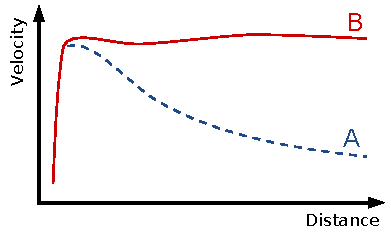
\includegraphics[width=0.45\textwidth]{graphics/bbn/galactic_rotation}
    \caption{Galactic rotation: Case A shows the expected behavior, case B the observed one. Credit: \href{https://en.wikipedia.org/wiki/Dark_matter}{Wikipedia}.}
    \label{fig:bbn:galactic_rotation}
\end{figure}



\subsection{Cosmic Microwave Background}

In the Big Bang model, the universe started from a very hot and dense state. One expected remnant of this state is a relic radiation that in fact was detected in 1965 by Arno Penzias and Robert Wilson \citep{penzias65}. The detection of this \ac{cmb} is one of the pillars supporting the Big Bang model to describe the origin of the universe. The origin of the \ac{cmb} will be discussed in further detail below.

The \ac{cmb} is a thermal blackbody radiation with a measured temperature of $2.72548 \pm 0.00057$\,K. The peak of this radiation is in the microwave range and cannot be observed from Earth. Space missions such as \href{https://map.gsfc.nasa.gov/}{\ac{wmap}} and \href{http://www.esa.int/Science_Exploration/Space_Science/Planck}{Planck} measured the \ac{cmb} in detail. A map of the \ac{cmb} is shown in Figure~\ref{fig:bbn:wmap_cmb}.
\begin{figure}[tb]
    \centering
    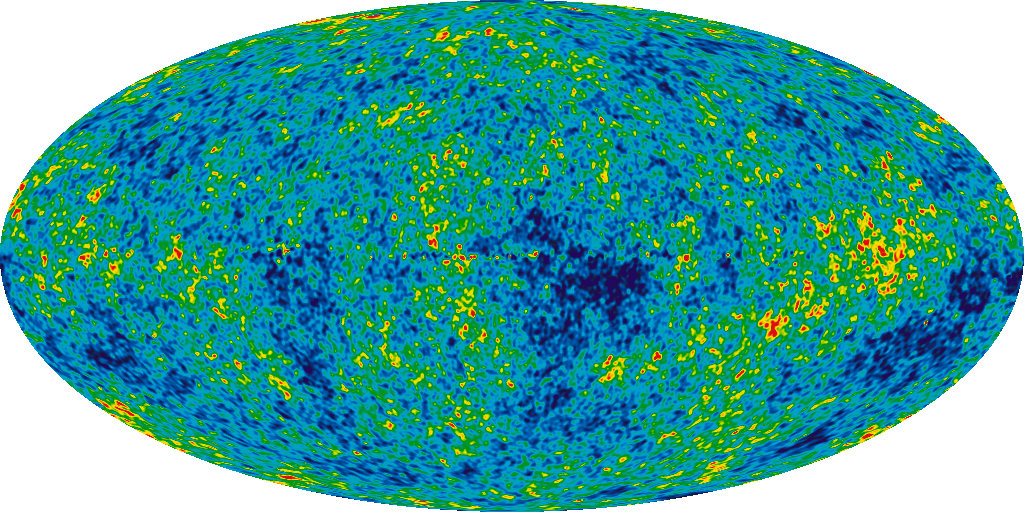
\includegraphics[width=0.75\textwidth]{graphics/bbn/wmap_cmb}
    \caption{\ac{wmap}'s image of the \ac{cmb}. Shown is averaged data from nine years of measurements. Credit: \href{https://map.gsfc.nasa.gov/media/121238/index.html}{NASA}.}
    \label{fig:bbn:wmap_cmb}
\end{figure}



\section{The Standard Model of Cosmology}

The standard model of cosmology describes the origin of the universe and its evolution based on one singular event: the Big Bang. With the Big Bang, space, time, and matter came into existence and the universe developed from its hot, dense state to the cold and transparent state we see today.

\subsection{Assumptions}\label{sec:bbn:standard_model:assumptions}

The standard model of cosmology is based on several key assumptions. Here we focus on the ones that are of importance to understand \ac{bbn}.

\begin{enumerate}
    \item The cosmological principle is valid. This states that the spatial distribution of matter in the universe in homogeneous and isotropic. \label{it:bbn:cosmological_principle}
    \item The overall charge in the universe is zero.
    \item The universe is made of matter and not of antimatter. This assumption in fact directly contradicts the cosmological principle (assumption \ref{it:bbn:cosmological_principle}) since it requires that there was an overabundance of baryons compared to antibaryons at the start of the universe, making it thus inhomogeneous. This overabundance of matter is to this date not fully explained and remains under active investigation.
    \item At temperature $T<10^{11}$\,K (approximately 10\,ms after the Big Bang), all heavy particles were annihilated and the density of the universe is defined by photons, neutrinos ($\nu$), electron and positrons ($\mathrm{e}^{\pm}$), and the remaining baryons.
\end{enumerate}


\subsection{Temperature and Density Evolution}

\begin{figure}[tb]
    \centering
    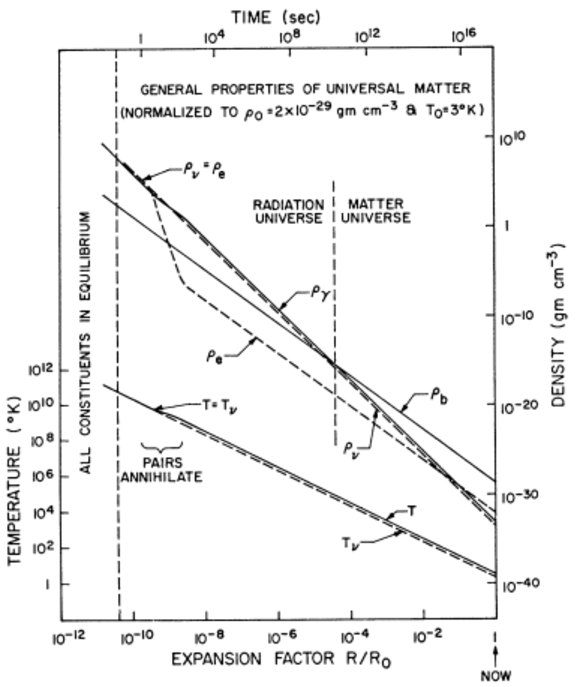
\includegraphics[width=0.6\textwidth]{graphics/bbn/wagoner67_fig1}
    \caption{The temperature and density evolution of the universe in the framework of the standard model of cosmology. Taken from \citet{wagoner67}. \copyright\ American Astronomical Society.}
    \label{fig:bbn:cosmology_phases}
\end{figure}
Figure~\ref{fig:bbn:cosmology_phases} shows the temperature and density evolution of the universe in the framework of the standard model of cosmology \citep{wagoner67}. The horizontal axis show the expansion factor $R/R_0$ as defined in equation \ref{eqn:bbn:redshift} on the bottom and the time since the Big Bang on the top. The vertical axes show the temperature (left) and the density (right). The standard model description starts at around 10\,ms with all constituents in equilibrium. \acl{bbn} sets in at a temperature of around $10^{9}$\,K. 



\section{Big Bang Nucleosynthesis}

\subsection{The Proton-to-Neutron Ratio}

In the beginning at a temperature of around $10^{11}$\,K (see Figure~\ref{fig:bbn:cosmology_phases}), the protons and neutrons are in thermodynamic equilibrium. Statistical mechanics shows that the energy of such a system can be expressed using the Boltzmann distribution for the individual states. This can be used to express the ratio of the number of protons to the number of neutrons in equilibrium conditions as
\begin{equation}\label{eqn:bbn:td_equilibrium_number_ratios}
    \left(\frac{n_\mathrm{p}}{n_\mathrm{n}}\right)_\mathrm{eq} 
        = \frac{\lambda_\mathrm{np}}{\lambda_\mathrm{pn}}
        = \exp\left(\frac{(m_\mathrm{n} - m_\mathrm{p})c^2}{kT}\right)
        = \exp\left(\frac{1.501}{T_{10}}\right).
\end{equation}
Here, $\lambda_\mathrm{np}$ and $\lambda_\mathrm{pn}$ are the reaction rates to turn a neutron into proton and vice verse, respectively. For $T\rightarrow\infty$ protons and neutrons will have equal abundances. At lower temperatures however, protons will become more abundant. 

We can rewrite equation~\eqref{eqn:bbn:td_equilibrium_number_ratios} to express the mass fractions of neutrons in equilibrium as
\begin{equation}
    X_\mathrm{n,eq} = \left(\frac{n_\mathrm{n}}{n_\mathrm{p} + n_\mathrm{n}}\right)_\mathrm{eq}
    = \frac{1}{(n_\mathrm{p} / n_\mathrm{n})_\mathrm{eq} + 1}
    = \frac{\lambda_\mathrm{pn}}{\lambda_\mathrm{pn} + \lambda_\mathrm{np}}.
\end{equation}


The nucleons react with each other via the weak force and the following reactions are possible:
\begin{eqnarray}
    \mathrm{n} + \nu &\longleftrightarrow& \mathrm{p} + \mathrm{e}^{-} \\
    \mathrm{n} + \mathrm{e}^{+} &\longleftrightarrow& \mathrm{p} + \bar{\nu} \\
    \mathrm{n} &\longrightarrow& \mathrm{p} + \mathrm{e}^{-} + \bar{\nu} \label{eqn:bbn:neutron_decay_reaction}
\end{eqnarray}
Reaction \eqref{eqn:bbn:neutron_decay_reaction} is the free decay of neutrons and has a half-life of 610\,s. This reaction can thus be neglected at the beginning since it is very long compared to all other reactions. The neutron mass fraction over time follows thus the differential equation
\begin{equation}
    \frac{d}{dt}X_\mathrm{n}(t) = -\lambda_\mathrm{np}(t)X_\mathrm{n}(t) + \lambda_\mathrm{pn}(t)[1-X_\mathrm{n}(t)].
\end{equation}
With decreasing temperature the reaction rates $\lambda_\mathrm{np}$ and $\lambda_\mathrm{pn}$ go rapidly towards zero such that after around 10\,s the proton to neutron ratio is frozen in place. Calculating reaction rate values, e.g., as in \citet{peebles66apj}, the neutron mass fraction at freezeout (when the reaction rates $\lambda_\mathrm{np}$ and $\lambda_\mathrm{pn}$ go to zero) is
\begin{equation}
    X_\mathrm{n,freeze} = 0.164.
\end{equation}
From this time on, the only reaction taking place is free neutron decay, see reaction~\eqref{eqn:bbn:neutron_decay_reaction}. Since the half-life of neutrons is fairly short, they must rapidly after the freezeout be captured as part of atomic nuclei in order to not decay away.


\subsection{Nucleosynthesis of Deuterium}

Deuterium has a mass of $m_\mathrm{D} = 1875.612928$\,MeV, while a proton and neutron have masses of $m_\mathrm{p} = 938.272088$\,MeV and $m_\mathrm{n} = 939.565421$\,MeV (see info box below for an explanation of measurements in eV).  
\begin{table}[b]  % since info boxes are in tabular environments...
\infobox{Measurements in eV}{In nuclear physics, masses are often expressed in mega electronvolts or MeV, which is technically not a mass but an energy. The mass of the particle is related to its energy via Einstein's equation $m=E/c^2$. Thus, energy and mass are directly related with $c$, the speed of light, as a proportionality constant. Similarly we can write the momentum of a particle as $\vec{p} = E \vec{c}^{-1}$ and the temperature of a system as $T = E k_B^{-1}$. Here, $k_B$ is the Boltzmann constant. Since mass, momentum, and temperature are related to energy via constants, these quantities are often expressed as energies.}
\end{table}
Deuterium, an isotope of hydrogen (\ex{2}H), consists of one proton and one neutron. However, summing the mass of one proton and one neutron results in a mass that is $\Delta m = 2.22$\,MeV larger than the mass of deuterium. This so-called mass defect defines the binding energy of deuterium and is the reason why energy is released when a proton and neutron are fused together. In chemistry this would be called an exothermic reaction. It can be written as
\begin{equation}\label{eqn:bbn:deuterium_formation_reaction}
    \mathrm{p} + \mathrm{n} \longrightarrow \mathrm{D} + \gamma.
\end{equation}
\begin{figure}[tb]
    \centering
    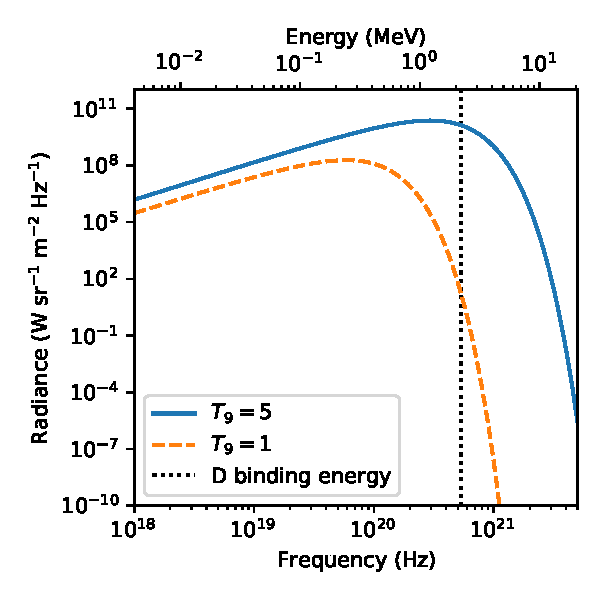
\includegraphics[width=0.5\textwidth]{graphics/bbn/planck_radiation_bbn}
    \caption{Spectral energy of black body radiation at the temperature when neutrons and protons are in equilibrium ($T_{9} \approx 5$) and when deuterium fusion can start ($T_{9}\approx1$). Prior to this temperature, the photon energies are too high and destroy newly formed deuterium effectively.}
    \label{fig:bbn:planck_radiation_deuterium_fusion}
\end{figure}

At the time when $n_\mathrm{p}/n_\mathrm{n}$ is frozen, the temperature of the universe is still $T\approx 5\times 10^{9}$\,K. Any deuterium that forms at this temperature is effectively destroyed right away again, since many photons have enough energy to dissociate the binding energy of 2.22\,MeV. Figure~\ref{fig:bbn:planck_radiation_deuterium_fusion} shows the spectral energy of a blackbody at this high temperature as a function of the frequency of the photons (bottom axis) and as function of their energy in MeV (top axis). The black, dashed line shows the deuterium binding energy. Note that both axes of the figure are logarithmic. Clearly, at $T_9 = 5$ many photons still have high enough energies. The universe thus first needs to cool down below $T_9 \approx 1$ before deuterium can effectively form. 

The exact temperatures, as just described, do not only depend on the temperature but also on the abundance of photons. Furthermore, the temperature is directly related to the density of the universe. Figure~\ref{fig:bbn:planck_radiation_deuterium_fusion} thus only gives a relative insight into the dissociation of deuterium. More detailed calculations can be found in the literature, e.g., in \citet{wagoner67}.

The drop in temperature of the universe from when proton and neutron abundances are frozen until deuterium can effectively form without being destroyed takes about 220\,s. During this time, the neutrons still undergo free decay. Using equation~\eqref{eqn:radioactive_decay} we can calculate that by the time deuterium fusion becomes significant, another $\sim20$\% of the neutrons decay.
This leaves behind a neutron fraction of
\begin{equation}
    X_n = 0.128
\end{equation}
at the start of \ac{bbn}.

\subsection{Nucleosynthesis of Helium}

Once deuterium has formed, more reactions can take place. Some of these reactions are:
\begin{eqnarray}
    \mathrm{D} + \mathrm{D} &\longleftrightarrow& ^3\mathrm{He} + \mathrm{n} \\
    \mathrm{T} + \mathrm{p} &\longleftrightarrow& ^3\mathrm{He} + \mathrm{n} \\
    \mathrm{T} + \mathrm{D} &\longleftrightarrow& ^4\mathrm{He} + \mathrm{n} \\
    \mathrm{p} + \mathrm{D} &\longleftrightarrow& ^3\mathrm{He} + \gamma \\
    \mathrm{n} + \mathrm{D} &\longleftrightarrow& \mathrm{T} + \gamma \\
    \mathrm{p} + \mathrm{T} &\longleftrightarrow& ^4\mathrm{He} + \gamma \\
    \mathrm{n} + {^3}\mathrm{He} &\longleftrightarrow& ^4\mathrm{He} + \gamma \\
    \mathrm{D} + \mathrm{D} &\longleftrightarrow& ^4\mathrm{He} + \gamma
\end{eqnarray}
Here, T is a tritium nucleus, another isotope of hydrogen with two neutrons (\ex{3}H). The reaction rates for these individual paths can be calculated, however, let us first estimate the dominant product of big bang nucleosynthesis. For deuterium above we determined a binding energy of 2.22\,MeV. Calculating the mass defect and thus the binding energy for \ex{3}He and \ex{4}He gives 6.70\,MeV and 27.3\,MeV, respectively. A better way to compare these binding energies is however to determine the binding energy per nucleon. For \ex{3}He and \ex{4}He these would be 2.23\,MeV per nucleon and 6.81\,MeV per nucleon. Thus, \ex{4}He is much favored to being produced. 

If we assume that all neutrons will be bound into \ex{4}He, a fairly accurate assumption as we will see further down, we can now predict the mass fraction of helium ($Y$) in the universe. After free decay of neutrons, we are left with $X_\mathrm{n} = 0.128$. Since \ex{4}He is roughly four times heavier than hydrogen, we can estimate the mass fraction of $^{4}$He as
\begin{equation}
    Y = \frac{4n_\mathrm{He}}{4n_\mathrm{He} + n_\mathrm{H}} 
        = \frac{2n_\mathrm{n}}{n_\mathrm{p} + n_\mathrm{n}}
        = \frac{2(n_\mathrm{n} / n_\mathrm{p})}{1+(n_\mathrm{n}/n_\mathrm{p})}
        = 0.23.
\end{equation}
This estimated value is in excellent agreement with the observed abundance of helium in the universe of about $1/4$ and is thus another robust pillar for the Big Bang model.


\subsection{Nucleosynthesis of heavier elements}

The highest binding energy per nucleon is found in the isotope \ex{62}Ni. However, several reasons contribute to the fact that \ac{bbn} cannot synthesize nuclides heavier than \ex{7}Li.

\begin{figure}[tb]
    \centering
    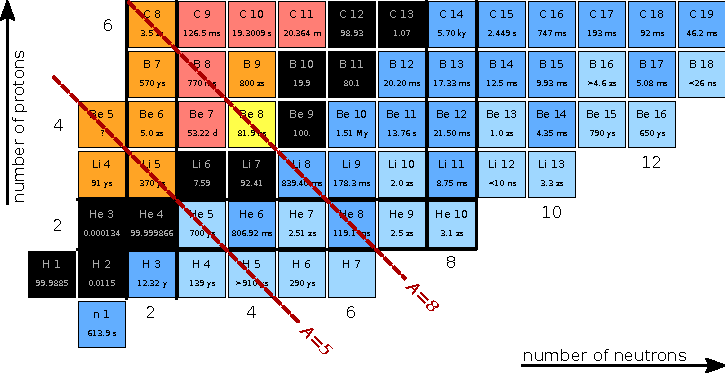
\includegraphics[width=0.85\textwidth]{graphics/bbn/chart_nuclides_bbn}
    \caption{The low-mass section of the chart of the nuclides with red, dashed lines indicating $A=5$ and $A=8$. These are the two mass regions that do not have any stable nuclides, thus effectively halting heavier element production in \ac{bbn}. Chart generated with a \href{https://github.com/kmiernik/Chart-of-nuclides-drawer}{python tool by Krzysztof Miernik}.}
    \label{fig:bbn:chart_nuclides_low_mass_region}
\end{figure}
Figure~\ref{fig:bbn:chart_nuclides_low_mass_region} shows an excerpt of the chart of the nuclides from hydrogen to carbon. Black isotopes are stable. The dashed, red lines indicate mass numbers $A=5$ and $A=8$, at which no stable nuclides exist. Thus, reactions of two \ex{4}He nuclei or a \ex{4}He nucleus and a proton do not form stable nuclides, which prevents \ac{bbn} from forming anything heavier than \ex{7}Li. 

While nucleosynthesis takes place, the universe continues expanding, thus the temperature further decreases. This significantly limits the time in which new nuclides can form. Below a temperature of $T_9\approx 0.1$ \ac{bbn} comes to a halt. This means that around 10-15\,min after the Big Bang, all the hydrogen, helium, and other \ac{bbn} products were formed. 

\begin{figure}[tb]
    \centering
    
\includegraphics[width=0.4\textwidth]{graphics/bbn/reaction_network}
    \caption{\ac{bbn} reaction rate network for dominant reactions, after \citet{nollett2000}.}
    \label{fig:bbn:reaction_network}
\end{figure}
Figure~\ref{fig:bbn:reaction_network} shows the reaction network showing dominant reactions at work in \ac{bbn} \citep[after][]{nollett2000}. As is common, we abbreviate the \ex{4}He nucleus with the symbol $\alpha$. Reactions are written in their abbreviated form, as is common in nuclear physics. For example \ex{1}H(n,$\gamma$)\ex{2}H could also be written as \ex{1}H + n $\longrightarrow$ \ex{2}H + $\gamma$. Notably, there is no main reaction to produce \ex{6}Li. Lithium-7 can be produced in two ways: directly from tritium by capturing a $\alpha$ particle (which is equivalent to \ex{4}He capturing a tritium nucleus) or by production of \ex{7}Be (from \ex{3}He) and subsequent decay to \ex{7}Li.


\subsection{Observational Constraints}

So far, we have roughly derived the production of hydrogen and \ex{4}He expected to form during the Big Bang. We furthermore mentioned how D, \ex{3}He, and \ex{7}Li are produced. Our derivations were mainly based on the temperature and density evolution of the universe during \ac{bbn}, two quantities that are coupled to each other. By observing the abundances of hydrogen, helium, and lithium in the universe and deriving the fractions of the species of interest that formed in the Big Bang, we can constrain the environment in which \ac{bbn} took place. 

\begin{figure}[tb]
    \centering
    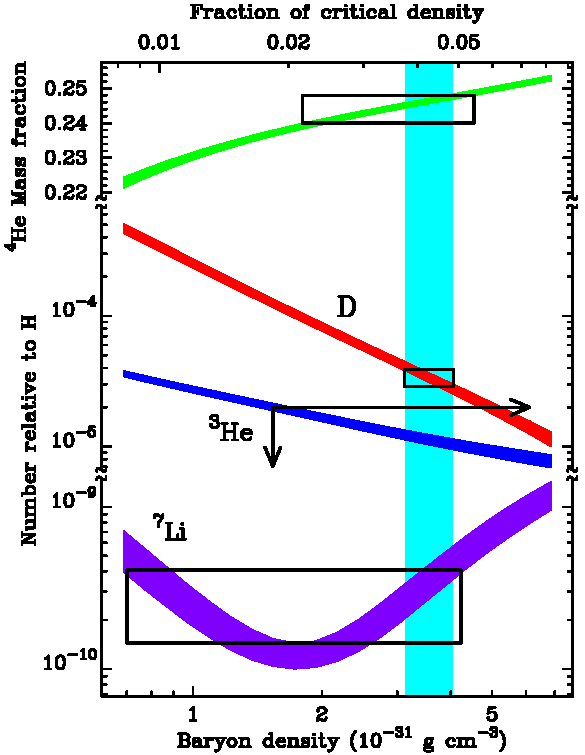
\includegraphics[width=0.5\textwidth]{graphics/bbn/tytler2000_fig2}
    \caption{\ac{bbn} predictions of the D, \ex{3}He, \ex{4}He, and \ex{7}Li abundance as a function of the present-day baryon density \citep{tytler20}. From \href{https://arxiv.org/abs/astro-ph/0001318}{\texttt{arXiv:astro-ph/0001318}}.}
    \label{fig:bbn:nuclides_baryon_density}
\end{figure}
Figure~\ref{fig:bbn:nuclides_baryon_density} shows the calculated abundances of D, \ex{3}He, \ex{4}He, and \ex{7}Li when varying the present-day baryon density. The squares show the observed ratios, where available, and their uncertainties. The larger the baryon density in the universe, the larger is the baryon-to-photon ratio. As discussed before, this ratio and the temperature define when deuterium can form (see Figure~\ref{fig:bbn:planck_radiation_deuterium_fusion}). If the baryon-to-photon ratio goes up, fewer neutrons decay until they are captured and thus more \ex{4}He nuclei are ultimately formed. The conversion of D to \ex{4}He will also be more complete, thus less deuterium remains. The higher starting abundance of D and higher end abundance of \ex{4}He also results in burning out \ex{3}He more effectively, thus lowering its abundance with an increase in the baryon density. The curve in Figure~\ref{fig:bbn:nuclides_baryon_density} for \ex{7}Li shows the competition of two reactions. At low baryon densities, \ex{7}Li is mainly produced via \ex{4}He + T $\longrightarrow$ \ex{7}Li + $\nu$. At increased baryon density, \ex{7}Li however gets again efficiently destroyed by burning further. This destruction is compensated and overtaken at even higher baryon densities since \ex{7}Be is produced more efficiently, which then immediately decays to \ex{7}Li.

While difficult to observe, the abundance of \ac{bbn}-produced hydrogen, helium, and lithium in the universe is a great way to determine crucial parameters of the Big Bang model. Similar insights can however also be gained by analyzing the \ac{cmb}.

\section{Recombination}

In Section~\ref{sec:bbn:standard_model:assumptions} we laid out the assumptions of the standard model of cosmology, one of which is that the overall charge in the universe is zero. During \ac{bbn}, the temperature too high to for electrons and nuclei to combine in order to produce a neutral gas. These components thus rather occur as a plasma. In order to create a neutral gas, the temperature has to sink to below $3000$\,K. At this temperature, the electrons combine with the atomic nuclei. Historically, this phase has been described as recombination, although the ``re'' part is slightly misleading since electrons and nuclei have never been combined previously.

During the plasma phase, i.e., prior to recombination, photons can scatter easily and the universe is thus opaque. After recombination the universe becomes transparent, and we transition into the matter dominated universe (see Figure~\ref{fig:bbn:cosmology_phases}). Since the Big Bang, roughly $4\times10^{5}$\,a have elapsed at this point.

The transition from the radiation dominated to the matter dominated universe can still be seen today as the horizon of the visible universe. It has significantly cooled down and is today seen as the \ac{cmb}. An image of is fluctuations is shown in Figure~\ref{fig:bbn:wmap_cmb}.


\section{Reading}

Since \ac{bbn} took place fairly long ago at this point, it seems adequate to also look at the literature from a historic point of view. For the historical perspective one should read \citet{alpher48} and \citet{peebles66prl}. These are both fairly short manuscripts. The present status of \ac{bbn} was recently given by \citet{cyburt16}. While this work contains fairly detailed methods on uncertainty calculations that are outside the scope of this lecture, please read sections III. Observations and V. The Lithium Problem in detail. You might also want to skim the introduction and the preliminaries.

For these readings it is important that you do not get hung up on details you do not understand, but rather try to follow the big picture. The following questions that can be discussed in class might help to focus on the big picture.

\begin{itemize}
    \item What elements and isotopes are all formed in the Big Bang according to the work by \citet{alpher48}? What are the issues you see with this model, especially regarding it from the current state of knowledge?
    \item What nuclides were produced in the Big Bang according to \citet{peebles66prl} and how does this differ from the work by \citet{alpher48}?
    \item Note the neutron half-life that is used in \citet{peebles66prl}. What is the issue here? This is also in detail discussed in the introduction by \citet{cyburt16}.
    \item What importance does the nuclear reaction rate network have in \citet{cyburt16}? What reaction rates are to this day fairly uncertain?
    \item Discuss how the primordial abundance of H, D, \ex{3}He, \ex{4}He, and \ex{7}Li can be derived from current observations. What are the problems?
    \item What is meant in \citet{cyburt16} by ``regression to zero metallicity''?
\end{itemize}
%!TEX root = origin_elements_lecture_notes.tex

\chapter{Star Formation}\label{sec:star_formation}

In the last chapter we discussed the formation of the first elements in the Big Bang and derived that all the hydrogen and the vast majority of helium we see today in the universe formed in this event. In this chapter we will study how stars can form from hydrogen and helium gas and how they evolve throughout their lifetime. This topic is discussed generally for all stars, however, we will in the end focus on the very first and oldest star to form in the galaxy.

\section{Molecular Cloud Collapse and Protostar Formation}

\begin{figure}[tb]
    \centering
    \begin{subfigure}{0.44\textwidth}
        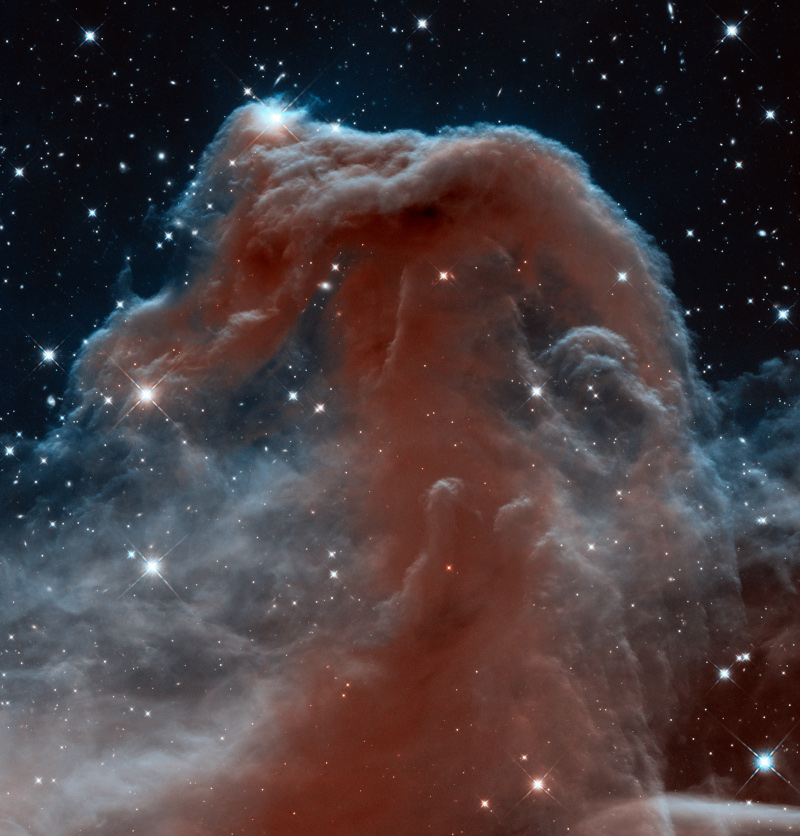
\includegraphics[width=\textwidth]{graphics/star_formation/horsehead_nebula}
        \caption{The horsehead nebula. Credit: NASA/ESA/Hubble Heritage Team.}
        \label{fig:star_formation:horsehead_nebula}
    \end{subfigure} \qquad
    \begin{subfigure}{0.459\textwidth}
        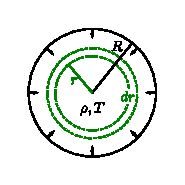
\includegraphics[width=\textwidth]{graphics/star_formation/molecular_cloud_collapse.pdf}
        \caption{A schematic representation of a molecular cloud collapsing.}
        \label{fig:star_formation:cloud_collapse_schematic}
    \end{subfigure}
    \caption{Molecular clouds are the structures stars form from in the universe.}
    \label{fig:star_formation:molecular_clouds}
\end{figure}
To understand star formation, let us first discuss how molecular clouds collapse. Figure~\ref{fig:star_formation:horsehead_nebula} shows a \ac{hst} image of the famous horsehead nebula, a molecular cloud located in the constellation Orion. Molecular clouds are accumulations of gas and dust in the galaxy that prevent light from the stars behind it to come through. These structures thus look like clouds to the observer.

\subsection{Jeans Criterium for Gravitational Collapse}

For simplicity, let us assume a spherical, homogeneous sphere with a constant density $\rho$ and temperature $T$. A schematic of such an idealized molecular cloud is shown in Figure~\ref{fig:star_formation:cloud_collapse_schematic}. The gravitational / potential that a given test mass $m$ in the molecular cloud is in can be written as
\begin{equation}
    E_\mathrm{pot} = -\frac{GMm}{R}.\label{eqn:star_formation:potential_energy}
\end{equation}
Here, $R$ is the distance of the test mass from the center of the molecular cloud and $M$ is the total mass of the cloud inside the radius $R$. Furthermore, $G$ is the gravitational constant and is equal to $G=6.674 \times 10^{11}$\,m$^{3}$\,kg$^{-1}$\,s$^{-2}$. Infinitely far away from the molecular cloud, the gravitational potential is by definition zero. Thus, it becomes negative the closer to the center the test mass gets. 

Instead of a test mass, let us now assume that we want to determine the gravitational energy of a mass shell with thickness $dr$ at distance $r$ from the center of the molecular cloud. A schematic of this setup is shown in Figure~\ref{fig:star_formation:cloud_collapse_schematic}. Assuming that the cloud is at a given temperature $T$ and has a homogeneous density $\rho$, we can write the mass of the shell ($m$) and the mass of the cloud inside the shell ($M$) as
\begin{eqnarray}
    m &=& 4 \pi \rho r^2 dr \label{eqn:star_formation:mass_molecular_cloud_shell} \\
    M &=& \frac{4}{3} \pi \rho r^3 \label{eqn:star_formation:mass_molecular_cloud}.
\end{eqnarray}
We can now determine the total potential energy of the molecular cloud as
\begin{equation}
    \begin{aligned}
        E_\mathrm{pot} &= -\int_0^R \frac{G}{r}\left( \frac{4}{3} \pi \rho r^3\right) \left( 4\pi \rho r^2\right) dr \\
        &=  -\frac{16}{3} \pi^2 \rho^{2} G \int_0^R r^4 dr \\
        &= -\frac{16}{15} \pi^2 \rho^2 GR^5 \\
        &= -\frac{3}{5}G\frac{M^2}{R}.
    \end{aligned}
    \label{eqn:star_formation:epot}
\end{equation}
In the last step we used the fact that the mass of the molecular cloud can be written as
\begin{equation}
    M = \frac{4}{3} R^3 \rho
\end{equation}
to substitute it back into the equation.

During the collapse, gravitational energy is transformed into kinetic energy, which here is equal to a rise in temperature. The total kinetic energy of the system can be written as
\begin{equation}
    E_\mathrm{kin} = \frac{3}{2} NkT = \frac{3}{2} kT \frac{M}{\mu}, \label{eqn:star_formation:ekin}
\end{equation}
where $N$ is the number of molecules in the molecular cloud and $\mu$ their average mass, i.e., to first approximation the mass of H$_2$.
For a cloud in hydrostatic equilibrium, i.e., a cloud that is neither expanding nor contracting, the virial theorem (which is derived in Appendix~\ref{app:virial_theorem}) can be applied. This theorem states that the kinetic and potential / gravitational energy are related to each other as
\begin{equation}
    2 E_\mathrm{kin} + E_\mathrm{pot} = 0. \label{eqn:star_formation:virial_theorem}
\end{equation}
Assuming the molecular cloud is in equilibrium, we can plug equations~\eqref{eqn:star_formation:epot} and~\eqref{eqn:star_formation:ekin} into~\eqref{eqn:star_formation:virial_theorem} and solve for the mass.
\begin{equation}
    \begin{aligned}
        3 kT \frac{M}{\mu} - \frac{3}{5}G \frac{M^2}{R} &= 0\\
        \frac{GM}{5R} &= \frac{kT}{\mu}\\
        M &= \frac{5RkT}{G\mu} \equiv M_J
    \end{aligned}\label{eqn:star_formation:jeans_mass_derivation}
\end{equation}
Here, $M_J$ is the so-called Jeans mass, named after Sir James Jeans who first described this derivation in 1904. It describes the mass $M=M_J$ for which the molecular cloud is in balance, i.e., the kinetic and gravitational energy compensate each other. The Jeans mass thus also describes the minimum mass for star formation; a molecular cloud with $M>M_J$ will collapse since the gravitational force dominates.


\subsection{Free Fall Time}

To determine how long gravitational collapse of a molecular cloud takes, we can estimate the free fall time. The gravitational force of the system and its radius are known. Using Newton's law $\vec{F} = m\vec{a}$, we can thus write the slightly unwieldy differential equation
\begin{equation}
    -G\frac{Mm}{R^2} = m\ddot{R},
\end{equation}
where $m$ is a test mass at the edge of the cloud. However, the free fall time $\tau_\mathrm{ff}$ can also be derived more elegantly. Kepler's third law of planetary motion states that the cube of the semi-major axis of a planet divided by the square of its period is constant. This law in fact can directly be derived by comparing the gravitational and centrifugal force acting on a planet since these two forces, for a stable orbit, must compensate each other.
\begin{figure}[tb]
    \centering
    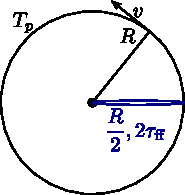
\includegraphics[width=0.3\textwidth]{graphics/star_formation/kepler3}
    \caption{Schematic to derive the free fall time $\tau_\mathrm{ff}$ using Kepler's third law of planetary motions. See text for details.}
    \label{fig:star_formation:kepler3_free_fall_time_schematic}
\end{figure}
Figure~\ref{fig:star_formation:kepler3_free_fall_time_schematic} shows a schematic of the here discussed scenario. The molecular cloud (black circle), if not collapsing, would have to rotate at a given velocity $v$ such that the gravitational force $F_\mathrm{g}$ and the centrifugal force $F_\mathrm{c}$ compensate each other. For a test mass at the outermost edge of the cloud, the gravitational force of the whole cloud is equivalent as if we pictured the mass of the cloud to be concentrated in the center. Disregarding vector quantities, we can derive the velocity a stable cloud would move around the center with as
\begin{equation}
    \begin{aligned}
        F_\mathrm{g} &= F_\mathrm{c} \\ 
        G\frac{Mm}{R^2} &= \frac{mv^2}{R}\\
        \Rightarrow v &= \left(G\frac{M}{R}\right)^{\nicefrac{1}{2}}.
    \end{aligned}
    \label{eqn:star_formation:velocity_orbit_stable_molecular_cloud}
\end{equation}
k
To determine the free fall scenario we can now halt the test particle in its motion, i.e., set $v=0$. The ``orbit'' of the test particle would then look like a straight line into the gravitational center of the cloud. In Figure~\ref{fig:star_formation:kepler3_free_fall_time_schematic} this scenario is shown by drawing the line as a very skinny ellipse. The semi-major axis of this orbit would now be $R/2$ and the orbital period $2\tau_\mathrm{ff}$. 

From Kepler's third law we know that the following statement must hold true.
\begin{equation}
    \frac{R^{3}}{T_P^2} = \frac{\left(\frac{R}{2}\right)^{3}}{(2\tau_\mathrm{ff})^2}
    \label{eqn:star_formation:kepler3_free_fall_time}
\end{equation}
Here, $T_P$ can be derived using the velocity as given in equation~\ref{eqn:star_formation:velocity_orbit_stable_molecular_cloud} and the length of the orbit ($2\pi R$). This yields
\begin{equation}
    T_p = 2\pi \left(\frac{R^{3}}{GM}\right)^{\nicefrac{1}{2}}.
    \label{eqn:star_formation:period_orbit_stable_molecular_cloud}
\end{equation}
Plugging equation~\eqref{eqn:star_formation:period_orbit_stable_molecular_cloud} into equation~\eqref{eqn:star_formation:kepler3_free_fall_time} and expressing the mass of the cloud using the density $\rho$ as $M=\frac{4}{3}R^3\rho \pi$, we can finally derive the free fall time as
\begin{equation}
    \tau_\mathrm{ff} = \left( \frac{3\pi}{32G\rho}\right)^{\nicefrac{1}{2}}.
\end{equation}


\subsection{Protostar Birth}

Fortunately, the molecular cloud collapse does not take place adiabatically. Heat is effectively radiated from the cloud as \ac{ir}, thus preventing the Jeans mass (which is proportional to the temperature) from exceeding the molecular cloud mass and thus bringing the cloud into hydrostatic equilibrium (see Section~\ref{sec:star_formation:hydrostatic_equilibrium}). The main cooling mechanisms producing \ac{ir} radiation are molecular collisions and dust. Colliding molecules transfer energy into vibrational states which, when they decay, emit \ac{ir}. Dust on the other hand will heat up and radiate as a blackbody with an effective temperature of less than around 1000\,K, thus mostly radiating in the \ac{ir}. The molecular cloud is mostly transparent to \ac{ir} and can thus effectively cool thanks to these processes.

Ultimately, the rising heat will start dissociating molecules and evaporating dust, thus the effective cooling mechanism stops. At this point the temperature in the center rises and the Jeans mass will be exceeded. The center of the collapsing cloud defines the protostar in hydrostatic equilibrium (see below).



\section{Hydrostatic equilibrium} \label{sec:star_formation:hydrostatic_equilibrium}

Once a molecular cloud has reached a high enough temperature such that its mass is equal to the Jeans mass, the system has entered the so-called hydrostatic equilibrium. Understanding this equilibrium is crucial in terms of understanding stellar phases during the end of their lives and during nucleosynthesis events. The whole life of a star is dominated by hydrostatic equilibrium. 

\begin{figure}[tb]
    \centering
    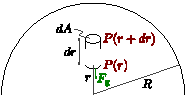
\includegraphics[width=0.4\textwidth]{graphics/star_formation/hydrostatic_equilibrium}
    \caption{Schematic drawing to derive the hydrostatic equilibrium equation. See text for details.}
    \label{fig:star_formation:hydrostatic_equilibrium_schematic}
\end{figure}
Figure~\ref{fig:star_formation:hydrostatic_equilibrium_schematic} shows a cylinder of length $dr$, face area $dA$, and density $\rho(r)$ at distance $r$ from the center of the star. The gravitational force that acts on the cylinder can be written as
\begin{equation}
    F_\mathrm{g} = -G\frac{M_r dm}{r^2},
    \label{eqn:star_formation:hydrostatic_equilibrium_gravitational_force}
\end{equation}
where $M_r$ is the mass of the star that is inside radius $r$ and $dm = \rho(r) dr dA$ is the mass of the cylinder. 


In addition, the cylinder is under pressure, i.e., the pressure $P(r+dr)$ from above it pushing it down and the pressure $P(r)$ from below it pushing it up. To force exerted by the pressure is 
\begin{equation}
    F_P = dPdA,
    \label{eqn:star_formation:hydrostatic_equilibrium_pressure_force}
\end{equation}
where $dP = P(r+dr) - P(r)$.

In order for the cylinder to be neutrally buoyant, i.e., to be in hydrostatic equilibrium, the gravitational force must exactly compensate the force exerted by the pressure. Setting equations~\eqref{eqn:star_formation:hydrostatic_equilibrium_gravitational_force} and~\eqref{eqn:star_formation:hydrostatic_equilibrium_pressure_force} equal plus some simple algebra, we can derive the hydrostatic equilibrium condition as
\begin{equation}
    \frac{dP}{dr} = -\rho(r) \frac{GM_r}{r^2}.
    \label{eqn:star_formation:hydrostatic_equilibrium}
\end{equation}

\subsection{Central Pressure}

Using equation~\eqref{eqn:star_formation:hydrostatic_equilibrium}, we can estimate the central pressure of a star by integrating over $r$. For this estimate, let us replace the density $\rho(r)$ with the mean density inside the star. This mean density can be expressed as
\begin{equation}
    \bar{\rho} = \frac{M}{\frac{4}{3} \pi R^3}.
\end{equation}
We can furthermore write $M_r$ as a function of the distance $r$ from the center of the star. Remember that $M_r$ simply represents the mass of the star inside of radius $r$, thus
\begin{equation}
    M_r = M(r) = \frac{4}{3} \pi r^3 \bar{\rho}.
\end{equation}
Plugging these two quantities into equation~\eqref{eqn:star_formation:hydrostatic_equilibrium} and integrating over $r$, the central pressure $P_c$ can be estimated as
\begin{equation}
    P_c = \frac{3}{8\pi}\frac{GM^{2}}{R^{4}}.
    \label{eqn:star_formation:central_pressure}
\end{equation}
We assumed here that the pressure at the surface of the star is zero, which is surely true when compared to the central pressure. In the case of the Sun, using equation~\eqref{eqn:star_formation:central_pressure} we can calculate a central pressure of $P_{c,\odot} \approx 10^{14}$\,Pa.

Note that the presented estimate of the central pressure of a star necessarily represents a lower limit. The reason for this is that we assumed a constant density throughout the star, which surely is not correct. The density will be significantly higher in the center of the star compared to the outer parts. This always increases the pressure compared to our estimate. To visualize why, imagine all the mass of the star was concentration within $R/2$. Integrating the pressure over the whole star using our estimate above would result in the same central pressure. However, from our visualization we know that the central pressure is concentrated in the inner half, thus integration of $r$ only needs to be done up to $R/2$ to determine the ``real'' central pressure. This value will necessarily be higher than what we estimated in equation~\eqref{eqn:star_formation:central_pressure}.

For the Sun, $\rho(r)$ needs to be modeled in order to exactly determine the actual pressure. Such models yield a central pressure for the Sun of $2.5\times10^{16}$\,Pa, which is two orders of magnitude higher than our lower limit estimate.


\subsection{Central Temperature}

From the estimated central pressure, we can estimate the central temperature of a star assuming that the equation of state of an ideal gas holds in this scenario. This equation takes the form
\begin{equation}
    pV = Nk_BT,
\end{equation}
where $p$ is the pressure, $V$ the volume, $N$ the number of particles, $k_B$ Boltzmann's constant, and $T$ the temperature. The number of particles that are in the gas can be expressed as $N=M/\mu$, where $\mu$ is the mean molecular weight of all particles. For a gas made of neutral hydrogen, the mean molecular mass per particle would be equal to the molecular mass of hydrogen $\mu_\mathrm{H}$. However, we know that the temperature within the Sun is so high that the hydrogen gas is fully ionized. Thus, we have twice as many particles (protons and electrons) to consider. Since electrons have significantly less mass than protons, the mean molecular mass of the gas inside a star can be estimated as $\mu = \mu_\mathrm{H}/2$. Using equation~\eqref{eqn:star_formation:central_pressure}, the central temperature of a star can now be written as
\begin{equation}
    T_c = \frac{P_c \mu}{\bar{\rho} k_B}.
    \label{eqn:star_formation:central_temperature}
\end{equation}
Here, we replaced $N$ with $M/\mu$, which results in $V/M$ in this equation. This is of course equal to the reciprocal of the mean density $\rho$.

For the Sun, using the above determined pressure, we can estimate a temperature in the center of $T_{c,\odot} \approx 10^{7}$\,K. Considering all the approximation that we made up to here, this number agrees strikingly well with the central temperature of the Sun.



\subsection{Sustaining a Star via Gravity}

Knowing the luminosity $L$ of a star, e.g., the luminosity of the Sun, which is $L_\odot = 3.828\times10^{26}$\,W, we can calculate how long the star would live if it its energy would solely originate from gravitational collapse. The total gravitational energy available in the system is already given in equation~\eqref{eqn:star_formation:epot}. Since the luminosity is simply energy per time, the total amount of time that a star's luminosity could be sustained by gravitational infall is
\begin{equation}
    t = \frac{E_\mathrm{g}}{L} = \frac{GM^2}{RL} \equiv t_\mathrm{KH}.
    \label{eqn:star_formation:kelvin_helmholtz_time}
\end{equation}
This time is also known as the Kelvin-Helmoltz time ($t_\mathrm{KH}$). 

For the Sun we can calculate that gravity alone would be able to sustain the current luminosity for a total of $t_\mathrm{KH} = 3\times10^{7}$\,a. This time is more than two orders of magnitude too short. Looking at the Earth's fossil record, clear evidence has been found for live on Earth as far back as 3.5\,Ga \citep{schopf07}. Dating meteorites furthermore yields a Solar System age of 4.567\,Ga. Thus, the Sun must be at least be 100 times older than indicated by the Kelvin-Helmholtz time and another energy source is required to hold up the hydrostatic equilibrium.


\subsection{Nuclear Reactions}

We estimated the temperature at the center of the Sun to be $T_c \approx 10^7$\,K, which is high enough to efficiently convert hydrogen to helium. Nuclear reactions are in fact the reason that stars can sustain the hydrostatic equilibrium. In Section~\ref{sec:bbn:nucleosynthesis_of_helium} we established that converting four hydrogen atoms into one helium atom releases $\Delta E = 28.3$\,MeV of energy. If all the hydrogen mass ($M_\mathrm{H}$) of a star is available as fuel to sustain the hydrostatic equilibrium, the star's lifetime could be calculated as
\begin{equation}
    t_\mathrm{nuc} = \frac{M_\mathrm{H} N_A \Delta E}{4\,m_\mathrm{H} L}.
\end{equation}
Here, $N_A$ is Avogadro's constant and $m_\mathrm{H} = 1.008\,$g\,mol$^{-1}$ the molecular mass of hydrogen.

For the Sun, considering that hydrogen makes up $\sim75$\% of its mass, we can calculate $t_\mathrm{nuc} \approx 10^{11}$\,a. However, not all the hydrogen is available as fuel since the Sun is not fully convective. Only around 10\% of the hydrogen mass are accessible by the core and can thus be transformed to helium to produce energy. This puts the Sun's life while sustaining hydrostatic equilibrium via hydrogen burning at about 10\,Ga, which means we have about 5\,Ga left.


\subsection{The Death of a Star}

When stars run out of fuel in the center, nuclear reactions can no longer be sustained and thus the radiation pressure falls away. The star is thus no longer in hydrostatic equilibrium since $dP/dr = 0$ in equation~\eqref{eqn:star_formation:hydrostatic_equilibrium}. Therefore, the system will start collapsing again due to gravitation. The temperature in the center of the star will rise further until the next burning stage can start, i.e., helium burning in the triple $\alpha$ process producing \ex{12}C. These reactions produce again radiation pressure, thus reestablishing the hydrostatic equilibrium. How many burning stages can be accessed by the star depends on the star's initial mass and will be discussed later. 

\codebox{Stellar evolution}{The evolution of stars is generally modeled using elaborate stellar evolution codes. Many different codes exist, however, one open-source stellar evolution code has recently be widely adopted. The \ac{mesa} code, developed by Bill Paxton at UCSB, has enabled many new research group to work on stellar evolution and its consequences. In fact, anybody can run and install \ac{mesa}, instructions can be found on the \href{http://mesa.sourceforge.net/}{\ac{mesa} website}. Note that while \ac{mesa} is simple to use, users still must have some basic understanding of stellar evolution. The \href{https://en.wikipedia.org/wiki/Garbage_in,_garbage_out}{garbage in, garbage out concept} applies to stellar evolution as well.}
    

\section{The Initial Mass Function}

Star formation can only take place if a molecular cloud exceeds the Jeans mass. The likelihood of star formation in a given location of the galaxy depends on the density of material in that specific place. Depending on the total mass of the molecular cloud, stars of different masses can form. The so-called \ac{imf} describes the number distribution of stars with different masses between $0.1\,M_\odot$ and $100\,M_\odot$ and has been derived from observations. 

\begin{figure}[tb]
    \centering
    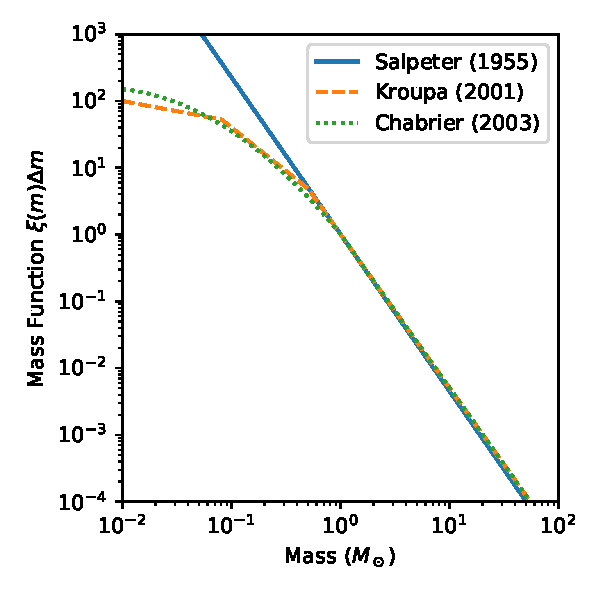
\includegraphics[width=0.5\textwidth]{graphics/star_formation/imf}
    \caption{Comparison of \acp{imf} by \citet{salpeter55}, \citet{kroupa01}, and \citet{chabrier03} normalized to $m=1\,M_\odot$.}
    \label{fig:star_formation:imf}
\end{figure}
Figure~\ref{fig:star_formation:imf} shows the \ac{imf} derived by three different researchers. The first \ac{imf} was published by \citet{salpeter55}. More detailed observations led to revisions of the \ac{imf} by \citet{kroupa01} and \citet{chabrier03}. 
For stars heavier than $1\,M_\odot$, all \acp{imf} agree with each other. At low masses, however, the \ac{imf} by \citet{salpeter55} significantly overestimates the abundance of stars compared to the predictions by \citet{kroupa01} and \citet{chabrier03}. Today, the latter two \acp{imf} are generally used for \ac{gce} models.


\section{The First Stars}\label{sec:star_formation:first_stars}

We have seen above that temperature and cooling play an essential role in star formation. The temperature of a molecular cloud is proportional to the Jeans mass, see equation~\eqref{eqn:star_formation:jeans_mass_derivation}. This leads to two issues: (1) The universe at the beginning was hotter, thus more mass is required for a molecular cloud to undergo gravitational collapse. (2) The main cooling processes of molecular clouds is to radiate heat away to not fall too early into hydrostatic equilibrium. This requires molecules and dust to be present. In the early universe the metallicity was however practically zero, thus this cooling process, except the dissociation of H$_2$ molecules, cannot take place. As a result only very massive, metal-free stars are expected to form in the beginning. 

These predicted, very massive stars with very low metallicity are called population III stars. Metal poor stars with $10^{-4}\,Z_\odot < Z < 10^{-5}\,Z_\odot$, which can mostly be found in old globular clusters, are called population II stars. All more metal-rich stars, mostly found in the galactic disk, are population I stars, e.g., the Sun.

Massive stars, as we will see in detail later on, have a much shorter lifespan than low-mass stars and will thus quickly enrich the early universe with freshly nucleosynthesized products, i.e., metals. Thus, second and later generation will start off with some metallicity. Possible nuclear reactions thus change and get more diverse. To study these earliest stars and nuclosynthesis events, spectroscopic observations of ultra metal-poor stars are an important part. 



\section{Reading}

For the curious reader, Anna Frebel wrote an excellent book titled ``Searching for the Oldest Stars'' \citep{frebel15}. The book is available via the Brandeis Library online.

For the discussion section we will focus on astronomical observations of Reticulum II, an ultrafaint dwarf galaxy that orbits the Milky Way. Please read \citet{croswell21}, a news feature article in the proceedings of the national academy of sciences. This article should give you a very brief and interesting overview of the field of the first stars, \ac{rproc} nuclei, and why they are important for understanding element formation in the universe. Furthermore, this brief article is written as a summary of recent events and discoveries.
Second, please read the paper by \citet{ji16} on the original observations of r-process enhanced stars in Reticulum II. This is the main article that we will discuss in class. The following bullet points should serve as guidance on reading these two manuscripts.
\begin{itemize}
    \item What are r-process nuclides and why are they important in this context?
    \item What are ultrafaint dwarf galaxies? Why are they so interesting when studying the oldest stars? What population of stars do these galaxies contain? What is special about Reticulum II?
    \item Why were neutron star mergers thought to be the main contributor to \ac{rproc} nuclei today, but not in the early universe? Has our thinking changed due to the work by \citet{ji16}? Has our thinking since then changed again?
    \item What is the difference between neutron-capture elements and non-neutron-capture elements? Why is this important in this context?
    \item Why do \citet{ji16} argue that all \ac{rproc} elements in Reticulum II were made by one single event?
    \item What is the neutron star merger to \ac{sn} rate ratio in the Milky Way? What factor do you think play into the determination of the rates?
    \item What alternative scenarios could explain the observations of \citet{ji16} aside from neutron star mergers?
\end{itemize}
%!TEX root = origin_elements_lecture_notes.tex

\chapter{The Life and Death of the Sun}\label{ch:sun}

In the last chapter we have seen how stars form from molecular clouds. We also derived the hydrostatic equilibrium, which is the conditions that stars spend most of their life in, and have analyzed some of its consequences. While we have already determined some key facts about the Sun, in this chapter we discuss the life of the Sun, its place among other stars in the Milky Way, and its ultimate fate in more detail. Understanding the Sun is useful; after all it is the energy source required for life on Earth. However, the Sun is also regularly used in comparison with other stars when discussing their lifetimes and fates.

\section{The Sun's Place in the Milky Way}

In Chapter~\ref{ch:solar_system_abundances} we have already discussed the place of the Sun in the Milky Way, see, e.g., Figure~\ref{fig:milky_way_profile_wiki}. Here, we will now also have a more detailed look at the Sun with respect to other stars -- its neighbors -- in the galaxy.

\subsection{The Hertzsprung-Russell Diagram}

\begin{figure}[p]
    \centering
    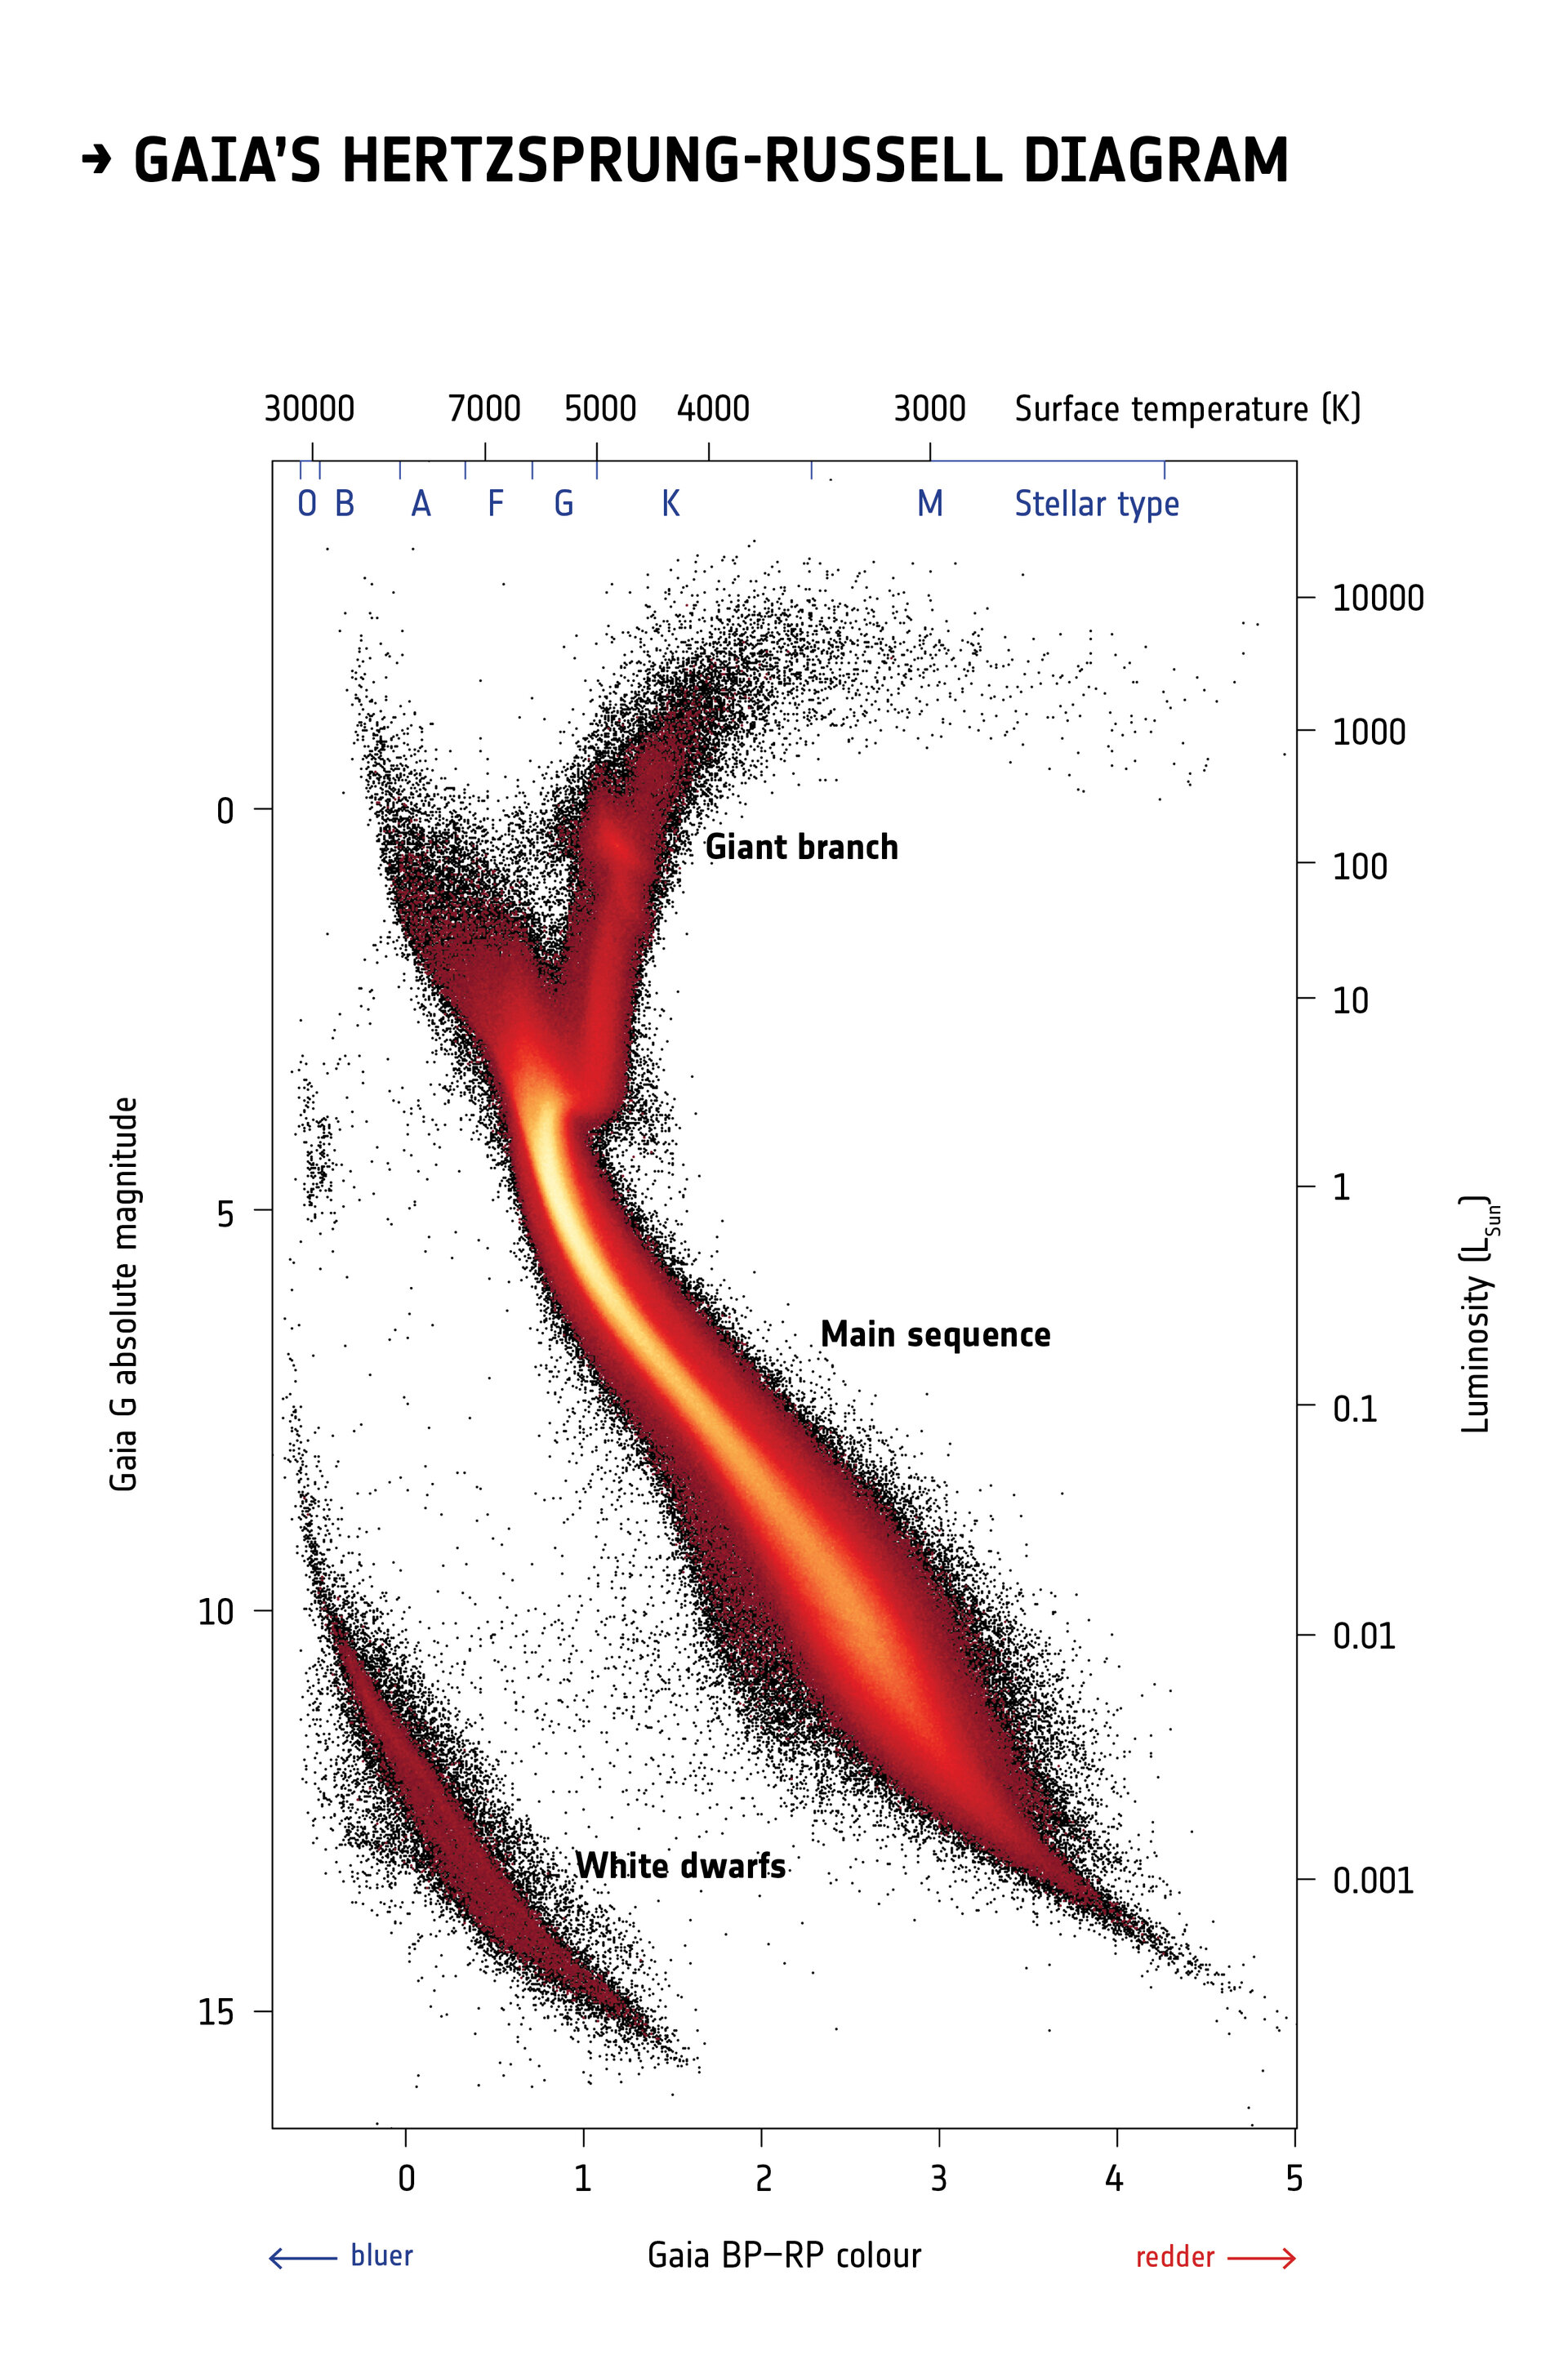
\includegraphics[width=0.81\textwidth]{graphics/sun/gaia_hrd}
    \caption{The \acl{hrd} put together from four million stars within 5000\,ly of the Sun. Credit: \acs{esa}/Gaia/DPAC, CC BY-SA 3.0 IGO.}
\label{fig:sun:hrd_gaia}
\end{figure}

Large-scale photographic and spectroscopic observations of stars led in the early 19$^\mathrm{th}$ century to the assembly of the first \ac{hrd}. An updated version of this diagram that includes around four million stars within 5000\,ly of the Sun is shown in Figure~\ref{fig:sun:hrd_gaia}. The observations for this \ac{hrd} were done with \href{https://sci.esa.int/web/gaia}{Gaia}, a space mission by the \ac{esa}. 

The \ac{hrd} originally showed the magnitude of a star, i.e., its brightness, versus its stellar type. While the brightness is directly related to the luminosity, the stellar type is related to the peak in its spectrum and thus to the star's surface temperature. Wien's displacement law (see Section~\ref{sec:solar_system_abundances:the_sun}) allows us to directly correlate the stellar type with the surface temperature of a star. Thus, the \ac{hrd} diagram plots the luminosity of a star, usually normalized to the solar luminosity $L_\odot$, with respect to its surface temperature.

Various notations exist for stellar types, see, e.g., \href{https://en.wikipedia.org/wiki/Stellar_classification}{here}. In Figure~\ref{fig:sun:hrd_gaia} the Harvard system is used, in which the stellar types from hottest to coldest stars are O, B, A, F, G, K, M (see the top axis of Figure~\ref{fig:sun:hrd_gaia}).

The Sun has a surface temperature of around $5800$\,K and is thus a G-type star. Knowing it's luminosity ($1\,L_\odot$), it's position in the \ac{hrd} can be identified. The Sun lays centered on a branch in the \ac{hrd} that is labeled as main sequence. The main sequence is the location in the \ac{hrd} where stars spend their lives, i.e., their quiescent burning phases. Once the nuclear fuel is exhausted, stars collapse further until the next burning stage can be activated. At this point, stars expand while keeping their surface temperature similar, thus they significantly increase their luminosity and wander up onto the giant branch. Finally, low mass stars end up as so-called \acp{wd}. These objects, usually surrounded by planetary nebulae, are compact and hot. Due to their small size, their luminosity is fairly low, which places them in the bottom left corner of the \ac{hrd}.

% \subsection{The Mass-Luminosity Relation}

\subsection{Planetary Systems}

With the discovery of the first exoplanet in 1995 by Michel Mayor and Didier Queloz of the Geneva Observatory, the Sun was suddenly not the sole star anymore that had planets orbiting it. The existence of other planets outside the Solar System has been long suspected; it is thought that Giordano Bruno (1548-1600), a Dominican monk, believed in a Copernican universe filled with an infinite number of inhabited worlds around other stars. While no evidence exists at this point for inhabited worlds, multiple exoplanets in the so-called Goldilocks or habitable zone have been discovered. These rocky planets are located at a distance from their parent star that allows for the existence of liquid water on the surface, like Earth. Note that while Mayor and Queloz received the 2019 Nobel Prize,\footnote{\url{https://www.nobelprize.org/prizes/physics/2019/summary/}} Bruno was executed for his beliefs. 

According to NASA's exoplanet website,\footnote{\url{https://exoplanets.nasa.gov/}} the current number of confirmed exoplanets as of \ExoplanetDate\ is \ExoplanetsNumber.
\begin{figure}[tb]
    \centering
    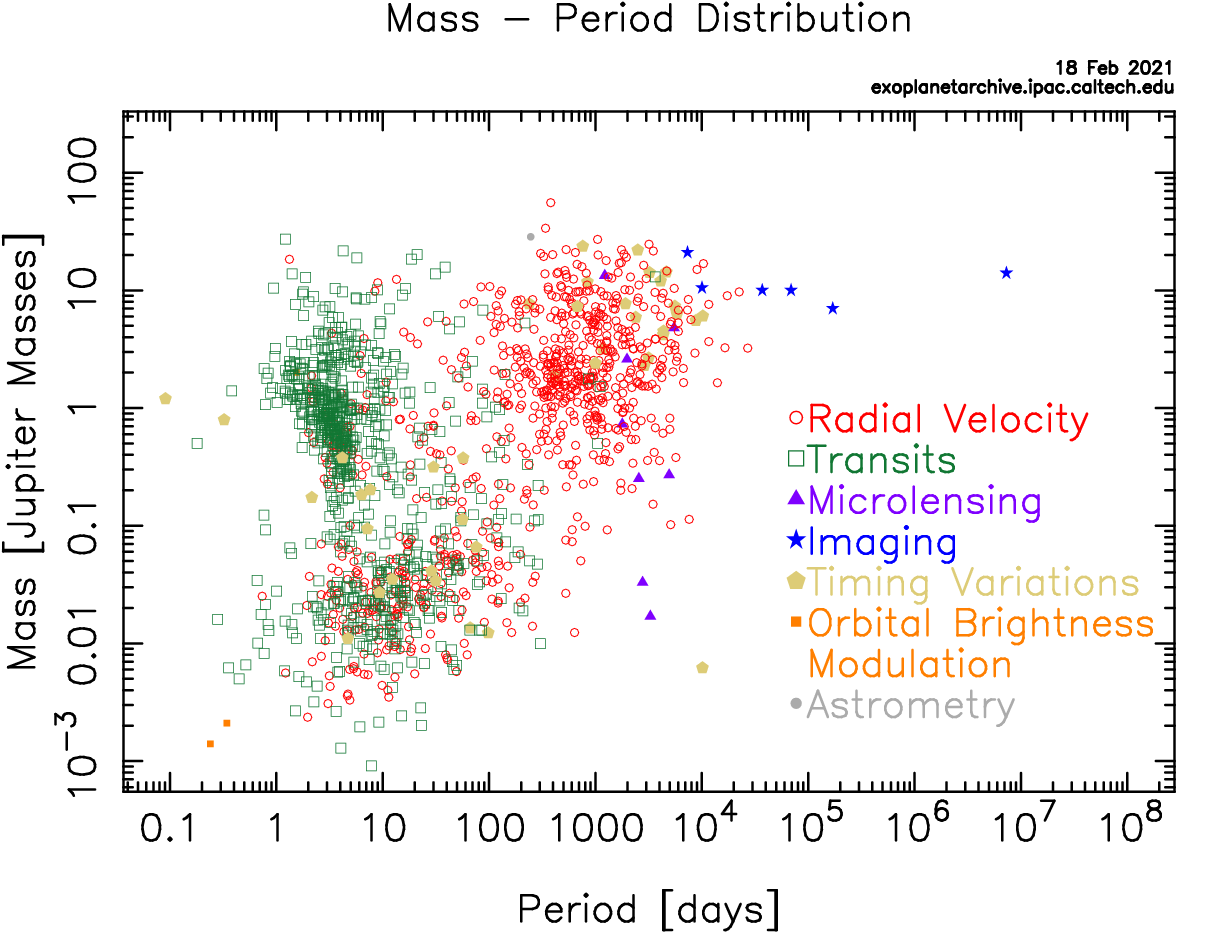
\includegraphics[width=0.75\textwidth]{graphics/sun/exoplanets_radius_period}
    \caption{Size of discovered expolanets as a function of their orbital periods. Source: \href{https://exoplanetarchive.ipac.caltech.edu/}{Exoplanet Archive, IPAC, Caltech}.}
    \label{fig:sun:exoplanets}
\end{figure}
Figure~\ref{fig:sun:exoplanets} shows a current figure for the size of confirmed exoplanets as a function of their orbital period. The size here is given in multiples of the size of Jupiter ($\jupiter$). Note that Earth ($\earth$) in this figure would plot at $M_{\earth} = 3.15 \times 10^{-3} M_{\jupiter}$ and at a period of 365\,d. Jupiter itself on the other hand, in comparison to other exoplanets, has an orbital period of 4333\,d. This shows that the Solar System seems to be an outlier when compared to all discovered exoplanets. Many of these exoplanets are heavy and orbit their parent star at short distances. Some massive exoplanets have orbital periods of a day and shorter. To what extent these discrepancies are due to observational bias remains under investigation, see, e.g., \citet{mulders18} and \citet{mulders19}.

\begin{table}[b]
\codebox{The Expolanet Population Observer Simulator (EPOS)}{is a python software package to simulate observations of expolanet populations. This package allows to study observational biases in transit and radial velocity exoplanet surveys, e.g., when analyzing data from the \href{https://www.nasa.gov/mission_pages/kepler/main/index.html}{Kepler} mission. The software package is well documented on \href{https://epos.readthedocs.io/en/latest/}{Read the Docs} and its source is available on \href{https://github.com/GijsMulders/epos/}{GitHub}.}
\end{table}


\subsection{Is the Sun Special?}

The Sun, overall, seems to be an average star like many others. While it plots in warmer areas of the \ac{hrd} than most stars that are on the main sequence, see Figure~\ref{fig:sun:hrd_gaia}, it is not outstandingly hot or cold. With respect to its planetary system it remains to be seen how common the Solar System as a whole is. Comparing the Solar System to exoplanets (Figure~\ref{fig:sun:exoplanets}) it seems as if we are fairly unique, however, this could simply be the result of observation biases since it is currently difficult to detect Earth-sized planets that orbit their parent star at distances of 1\,AU from their parent star. However, the habitable zone of a star of course does not just depend on the distance but also on the star's luminosity. 

The Sun is special in one aspect that has not been discussed so far, namely, it does not have a companion star. More than half of all stars are part of multiple star systems. As we will see later, these systems can have a significant effect on the stellar evolution and nucleosynthesis, and in some cases even be crucial for the production of certain elements.



\section{The Sun's Quiescent Burning Phase}

After having formed from a collapsing molecular cloud, the Sun entered the main sequence of the \ac{hrd} once nuclear fusion of hydrogen became the dominant heat source. Astronomers also refer to a star at the point when it enters the main sequence as a \ac{zams} star. From here on, the quiescent burning phase starts, in which stars slowly fuses hydrogen to helium. The \ac{hrd} in Figure~\ref{fig:sun:hrd_gaia} shows that most stars lay on the main sequence. The reason for this is that hydrogen burning is the longest phase a star goes through.

The four-body reaction 4 \ex{1}H \textrightarrow\ \ex{4}He + $\gamma$ is extremely unlikely to happen. Hydrogen fusion rather takes place in stages. Multiple processes are responsible as outlined below.

\subsection{The Proton-Proton-Chain}

\begin{figure}[tb]
    \centering
    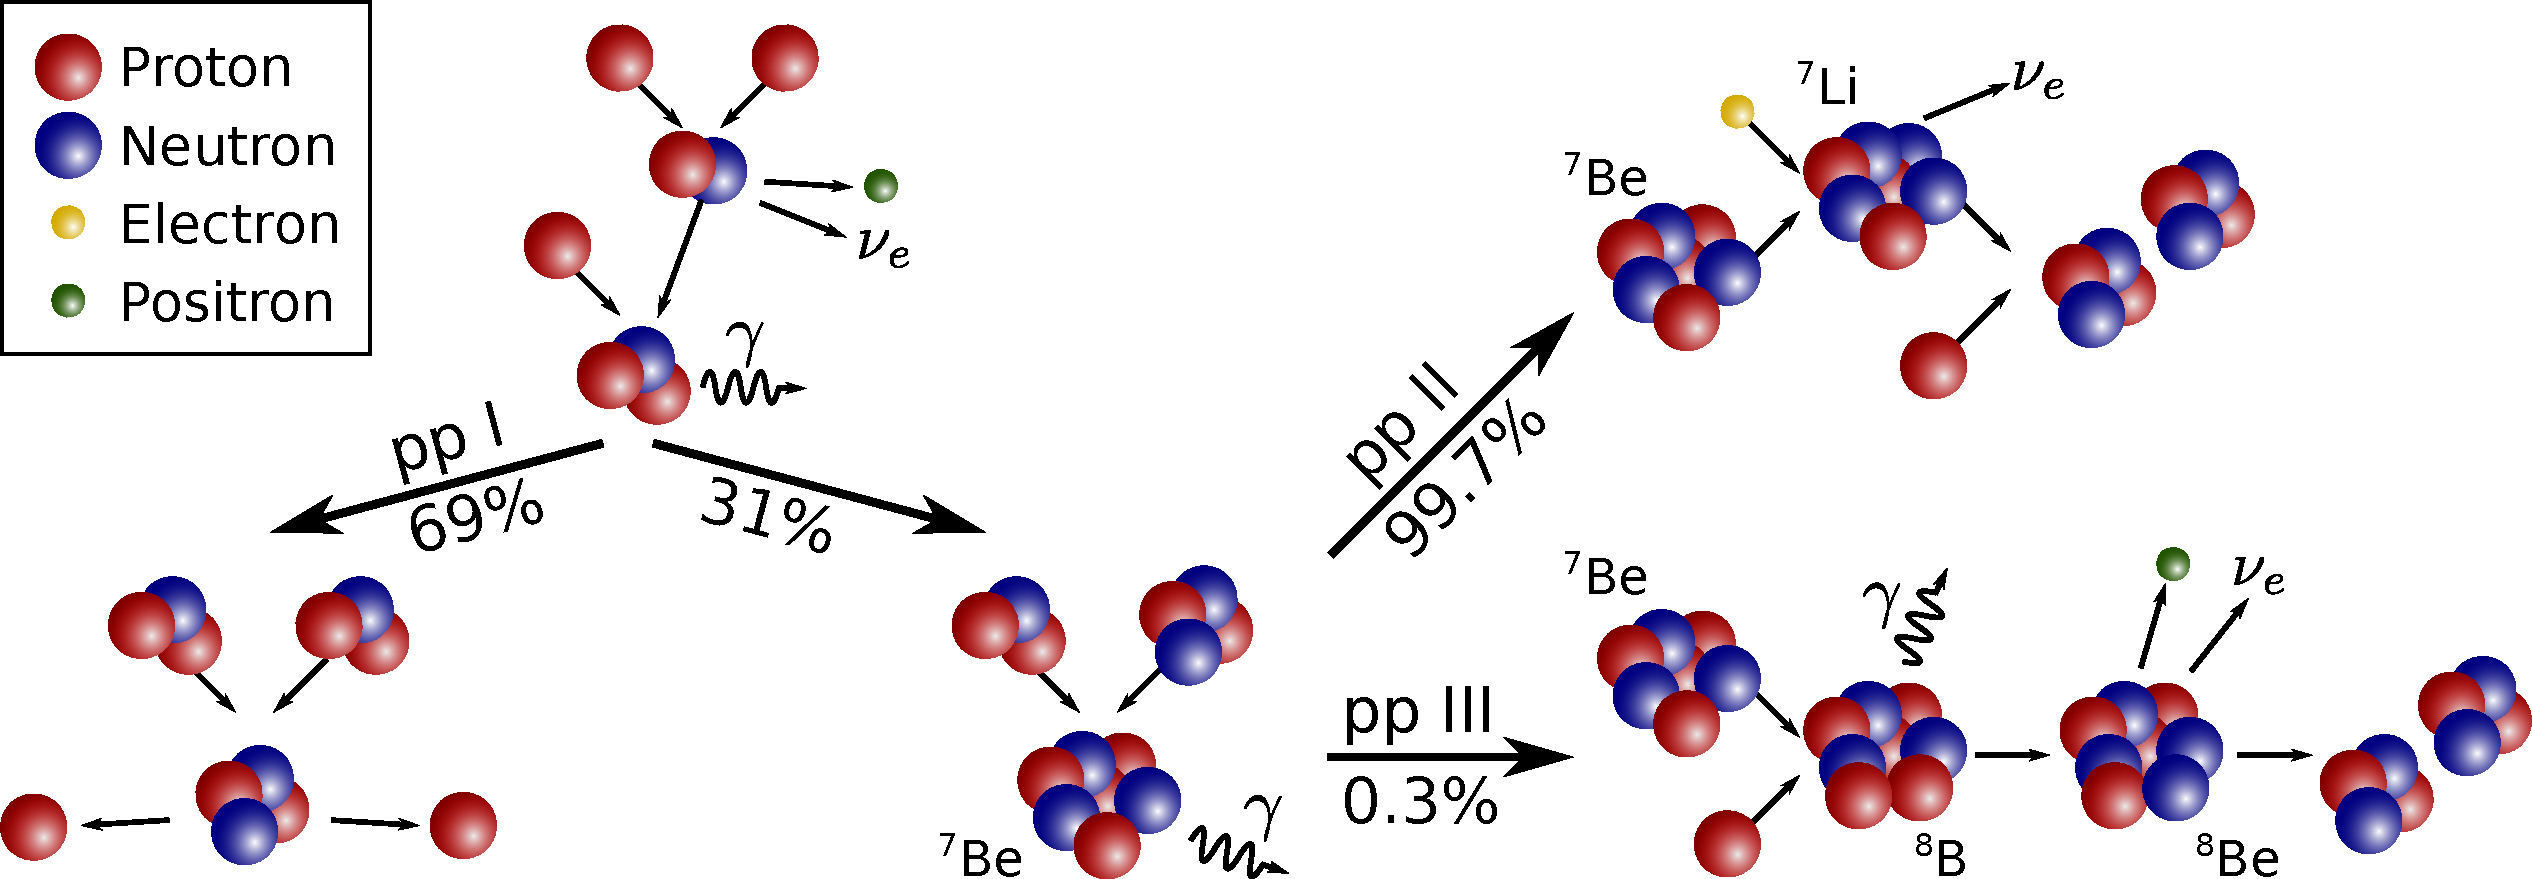
\includegraphics[width=\textwidth]{graphics/sun/pp_chain}
    \caption{The \ac{pp-chain} and it's three branches. Percentages are with respect to hydrogen fusion in the Sun.}
    \label{fig:sun:pp-chain}
\end{figure}
The \ac{pp-chain} is the main reaction chain that fuses hydrogen to helium in the Sun. Figure~\ref{fig:sun:pp-chain} shows a schematic of the \ac{pp-chain} and its three main branches. All branches start out with the reactions
\begin{align}
    {^1}\mathrm{H} + {^1}\mathrm{H} &\longrightarrow {^2}\mathrm{H} + \nu_e + e^+ \\
    {^2}\mathrm{H} + {^1}\mathrm{H} &\longrightarrow {^3}\mathrm{He} + \gamma.
\end{align}
Three protons are thus converted via deuterium (\ex{2}H) into a \ex{3}He nucleus. At this point the \ac{pp-chain} branches. The pp I chain, which is responsible for 69\% of the energy produced in the Sun via the \ac{pp-chain}, fuses two \ex{3}He nuclei and forms one \ex{4}He nucleus in the
\begin{equation}
    {^3}\mathrm{He} + {^3}\mathrm{He} \longrightarrow {^4}\mathrm{He} + 2\,{^1}\mathrm{H}
\end{equation}
reaction.

On the other branch in the \ac{pp-chain}, which takes place 31\% of the time in the Sun, a \ex{3}He and a \ex{4}He nuclei are first combined to form \ex{7}Be. The reaction is
\begin{equation}
    {^3}\mathrm{He} + {^4}\mathrm{He} \longrightarrow {^7}\mathrm{Be} + \gamma. \label{eqn:sun:pp-chain:intermediate_second_branch}
\end{equation}
Two paths are possible from here. The pp II chain forms \ex{4}He via the following reactions from \ex{7}Be:
\begin{align}
    {^7}\mathrm{Be} + e^{-} &\longrightarrow {^7}\mathrm{Li} + \nu_e \\
    {^7}\mathrm{Li} + {^1}\mathrm{H} &\longrightarrow 2\,{^4}\mathrm{He}
\end{align}
The \ex{4}He nucleus that is consumed in reaction~\eqref{eqn:sun:pp-chain:intermediate_second_branch} is gained back in the end. The pp II chain takes place 99.7\% of the time after the first branching.

The rest of the time in this second branch, the pp III chain produces \ex{4}He from \ex{7}Be. The reactions that take place are as following:
\begin{align}
    {^7}\mathrm{Be} + {^1}\mathrm{H} &\longrightarrow {^8}\mathrm{B} + \gamma \\
    {^8}\mathrm{B} &\longrightarrow {^8}\mathrm{Be} + e^+ + \nu_e\\
    {^8}\mathrm{Be} &\longrightarrow 2\,{^4}\mathrm{He}
\end{align}
The latter two reactions are here simply the decays of \ex{8}B and \ex{8}Be to form two \ex{4}He. Thus, the \ex{4}He consumed after the first branching is again gained back plus an additional \ex{4}He forms.

The nuclear energy generation rate in W\,kg$^{-1}$, simplified after equation~(10.46) in \citet{carroll17} (page 311), can be written as
\begin{equation}
    \epsilon_\mathrm{pp} = 0.241 \rho X^2 T_6^{-\nicefrac{2}{3}} \exp\left(-33.8 T_6^{-\nicefrac{1}{3}}\right). \label{eqn:sun:energy_generation_pp-chain}
\end{equation}
Here, $\rho$ is the density of the star's center and $T_6$ is the temperature expressed in multiples of $10^6$\,K. Assuming a density in the center of the Sun of $\rho = 150\,\mathrm{g}\,\mathrm{cm}^{-2}$, we can calculate the energy production of the \ac{pp-chain} at $\epsilon_\mathrm{pp} = 3.4 \times 10^{-3}\,$W\,kg$^{-1}$.


\subsection{The CNO-Cycle}
\begin{figure}[tb]
    \centering
    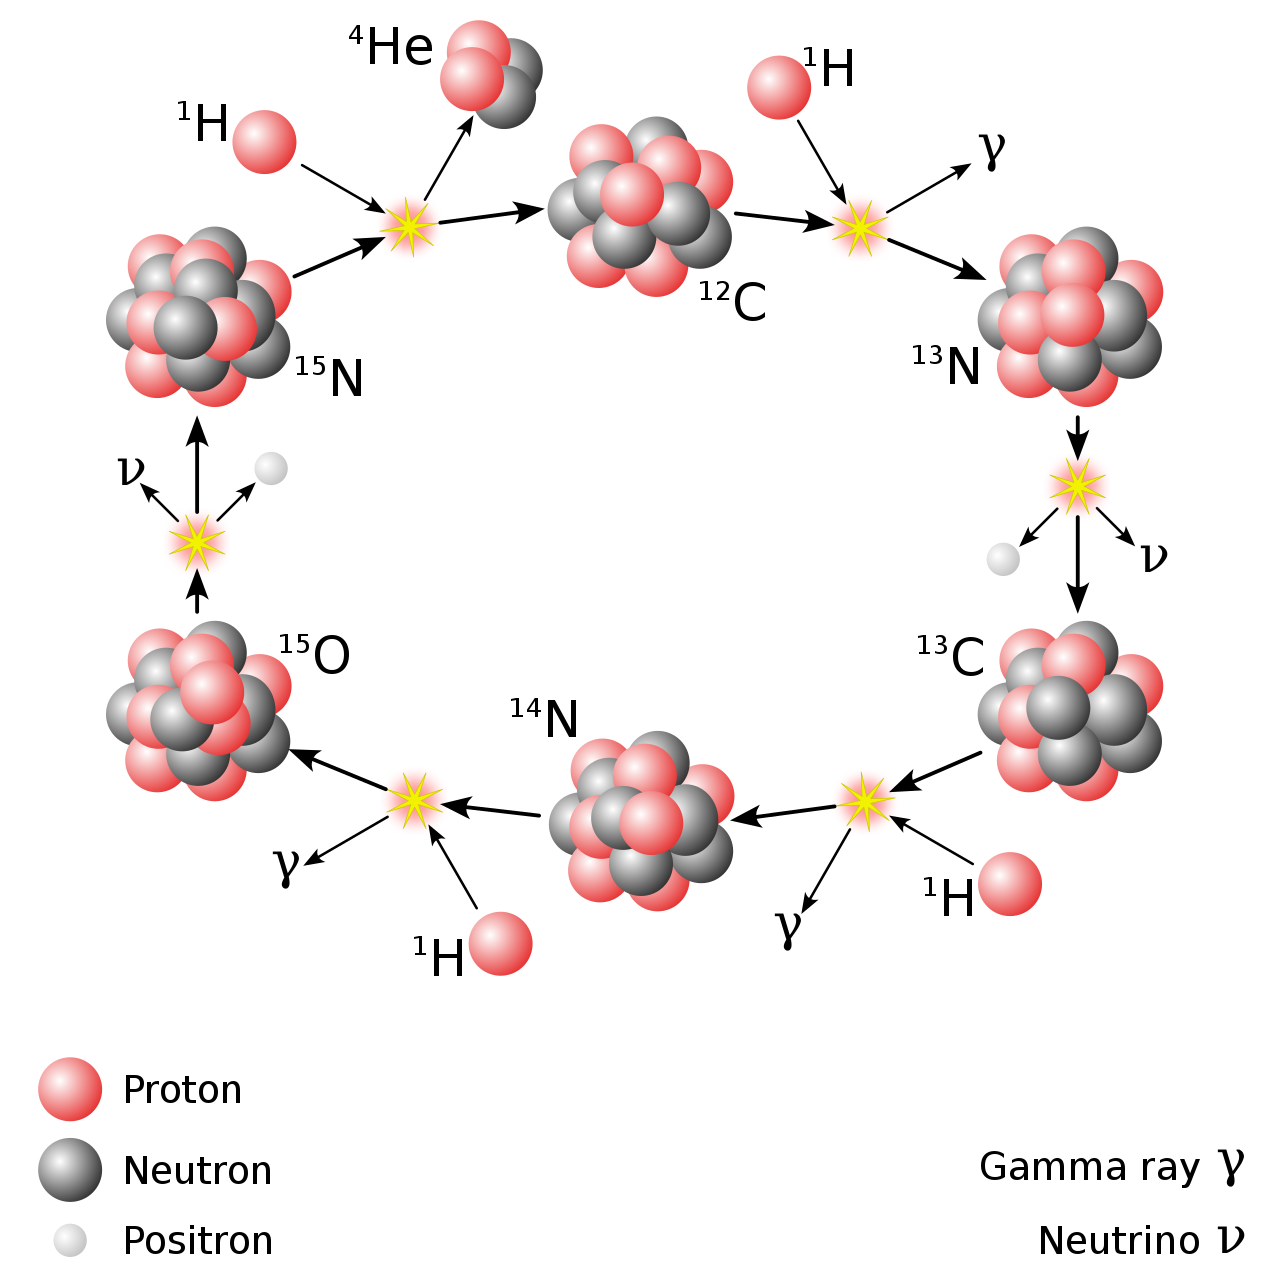
\includegraphics[width=0.6\textwidth]{graphics/sun/cno_cycle}
    \caption{Schematic drawing of the CNO cycle and the involved reactions. A \ex{4}He nucleus forms by combining four protons. The elements carbon, nitrogen, and oxygen act as catalysts for the reactions. Credit: \href{https://en.wikipedia.org/wiki/CNO_cycle}{Wikipedia}.}
    \label{fig:sun:cno_cycle}
\end{figure}
Compared to the \ac{pp-chain}, the CNO cycle requires carbon, nitrogen, and oxygen as catalysts for the reaction in order to combine four hydrogen nuclei into \ex{4}He. Figure~\ref{fig:sun:cno_cycle} shows a schematic of the CNO cycle. Starting at \ex{12}C, the involved reactions are as following:
\begin{align}
    {^{12}}\mathrm{C} + {^1}\mathrm{H} &\longrightarrow {^{13}}\mathrm{N} + \gamma\\
    {^{13}}\mathrm{N} &\longrightarrow {^{13}}\mathrm{C} + e^+ + \nu_e \\
    {^{13}}\mathrm{C} + {^1}\mathrm{H} &\longrightarrow {^{14}}\mathrm{N} + \gamma\\
    {^{14}}\mathrm{N} + {^1}\mathrm{H} &\longrightarrow {^{15}}\mathrm{O} + \gamma \label{eqn:sun:cno_cycle_n14_consumption}\\
    {^{15}}\mathrm{O} &\longrightarrow {^{15}}\mathrm{N} + e^+ + \nu_e\\
    {^{15}}\mathrm{N} + {^1}\mathrm{H} &\longrightarrow {^{12}}\mathrm{C} + {^4}\mathrm{He} \label{eqn:sun:cno_cycle_last_reaction}
\end{align}

As in the \ac{pp-chain}, the CNO cycle is also branched. This branch occurs at the last reaction~\eqref{eqn:sun:cno_cycle_last_reaction} and occurs only about 0.04\% of the time. The branch starting at reaction~\eqref{eqn:sun:cno_cycle_last_reaction}, which is not shown in Figure~\ref{fig:sun:cno_cycle}, is
\begin{align}
        {^{15}}\mathrm{N} + {^1}\mathrm{H} &\longrightarrow {^{16}}\mathrm{O} + \gamma\\
        {^{16}}\mathrm{O} + {^1}\mathrm{H} &\longrightarrow {^{17}}\mathrm{F} + \gamma\\
        {^{17}}\mathrm{F} &\longrightarrow {^{17}}\mathrm{O} + e^+ + \nu_e\\
        {^{17}}\mathrm{O} + {^1}\mathrm{H} &\longrightarrow {^{14}}\mathrm{N} + {^4}\mathrm{He}.
\end{align}
This branch thus does not drop back to \ex{12}C but rather produces \ex{14}N, which is also part of the CNO cycle and will be consumed further, see reaction~\eqref{eqn:sun:cno_cycle_n14_consumption}.

The nuclear energy generation rate in W\,kg$^{-1}$, simplified after equation (10.58) in \citet{carroll17} (page 312), can be written as
\begin{equation}
    \epsilon_\mathrm{CNO} = 8.67\times 10^{20} \rho X X_\mathrm{CNO} T_6^{-\nicefrac{2}{3}} \exp\left(-152.28 T_6^{-\nicefrac{1}{3}}\right). \label{eqn:sun:energy_generation_cno_cycle}
\end{equation}
Here, $X_\mathrm{CNO}$ is the mass fraction of CNO elements, i.e., the elements that are used as catalysts. In order for the CNO cycle to take place in a star, some metals must be present. For the Sun, the energy generation rate via the CNO cycle can be estimated as $\epsilon_\mathrm{CNO} = 2.3\times10^{-4}$\,W\,kg$^{-1}$.


\subsection{Energy Production in the Sun}

\begin{figure}[tb]
    \centering
    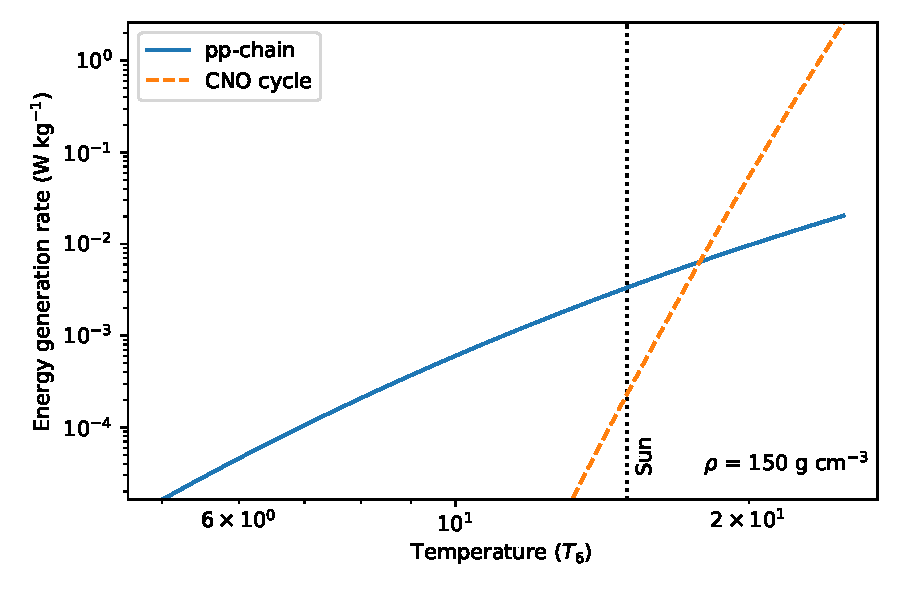
\includegraphics[width=0.75\textwidth]{graphics/sun/energy_h_burning}
    \caption{Energy generation rate due to the \ac{pp-chain} and CNO cycle as a function of temperature. The core density here is fixed to 150\,g\,cm$^{-3}$, which is approximately the density in the Sun's core.}
    \label{fig:sun:energy_generation_hydrogen_fusion}
\end{figure}
Figure~\ref{fig:sun:energy_generation_hydrogen_fusion} shows the energy generation rates of the \ac{pp-chain} and the CNO cycle (equations~\eqref{eqn:sun:energy_generation_pp-chain} and~\eqref{eqn:sun:energy_generation_cno_cycle}, respectively) as a function of the central temperature. A dotted line is shown at the Sun's central temperature. While the figure is scaled to the Sun's core density of $\rho\approx150$\,g\,cm$^{-3}$, both energy generation rates for the \ac{pp-chain} and the CNO cycle are proportional to $\rho$, thus the relative position of the two curves will stay the same for different stars and only depend on the temperature. 

Figure~\ref{fig:sun:energy_generation_hydrogen_fusion} clearly shows that the \ac{pp-chain} is the dominant energy source in the Sun. The CNO cycle's energy generation rate is more than an order of magnitude lower. However, at slightly higher temperatures, the CNO cycle will be the dominant source of nuclear energy that keeps a star in hydrostatic equilibrium.

In Section~\ref{sec:star_formation:first_stars} we discussed star formation at zero metallicity and concluded that these stars must have been very massive since cooling rates for molecular clouds are minimal at zero metallicity. If a star starts with $Z=0$, it can also only produce energy in its core via the \ac{pp-chain}. In Figure~\ref{fig:sun:energy_generation_hydrogen_fusion} it can be seen that the energy generation rate increases slower for the \ac{pp-chain} as a function of temperature compared to the CNO cycle. Thus, stars that start of with truly no metals must have gravitationally collapsed further until the temperature was high enough for the \ac{pp-chain} to compensate this infall and go into hydrostatic equilibrium.


\section{The Dying Sun}

\begin{figure}[bt]
    \centering
    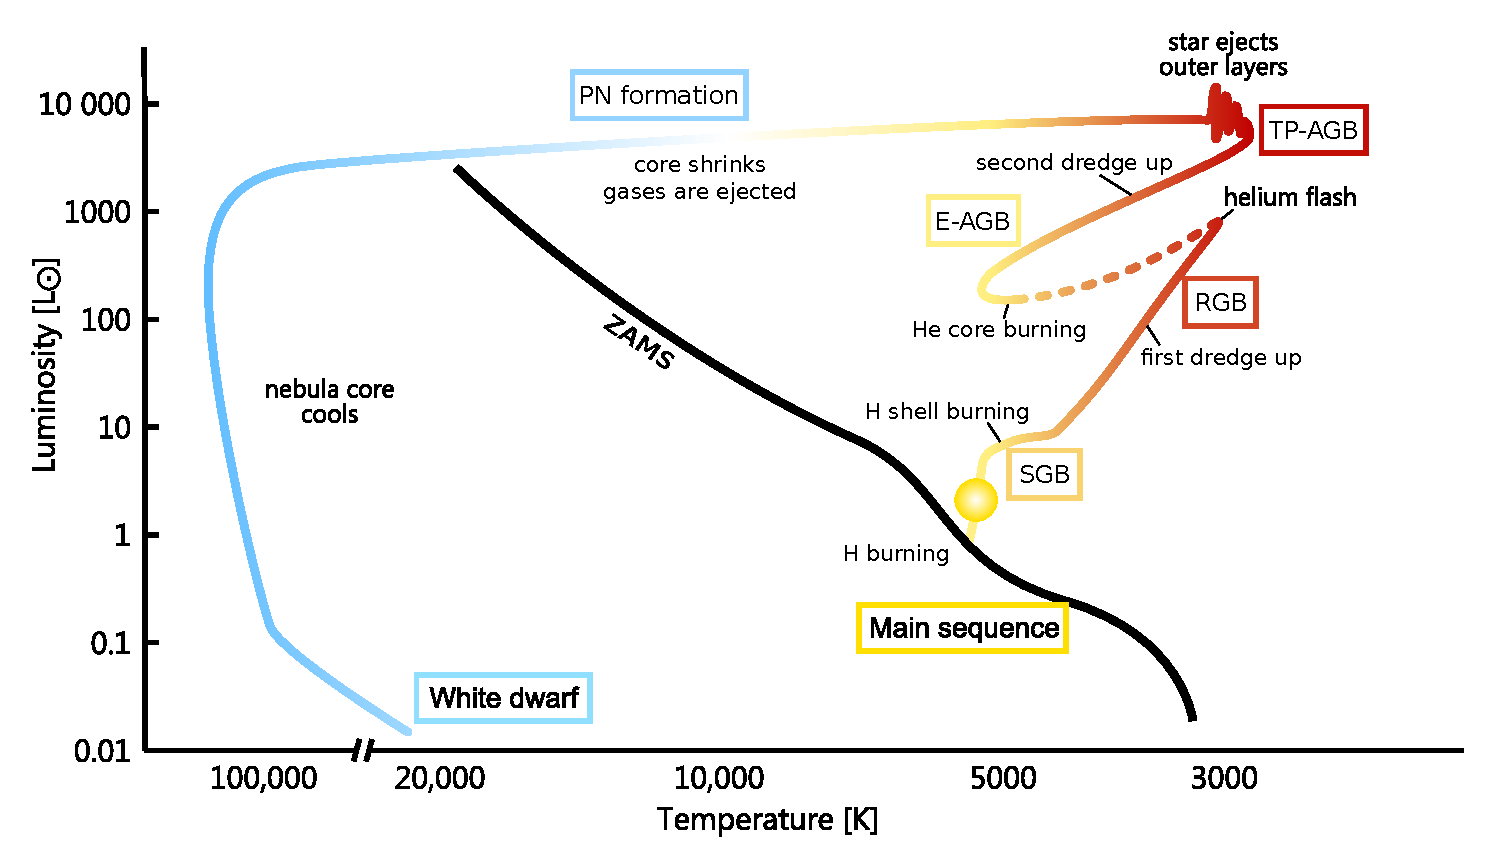
\includegraphics[width=0.9\textwidth]{graphics/sun/sun_hrd}
    \caption{Schematic of the evolution of the Sun in the \ac{hrd}. Figure adopted after \href{https://commons.wikimedia.org/wiki/File:Evolution_of_the_Sun_2_EN.svg}{Szczureq via Wikipedia Commons.}}
    \label{fig:sun:sun_hrd}
\end{figure}
Figure~\ref{fig:sun:sun_hrd} shows the evolution of the Sun in the \ac{hrd}. The black line in the background represents the \ac{zams} and here is where the Sun starts its life. Currently, the Sun is still on the main sequence quiescently burning hydrogen, as discussed above. While on the main sequence, the Sun is slowly moving upwards in the \ac{hrd} since continuous hydrogen burning slowly changes the average composition of the core. At present, about half of the nuclear fuel in the core has been consumed. Since the Sun has currently only at the surface a convective region, further hydrogen from the envelope is not accessible as fuel for hydrogen fusion. 

Note that the discussion here follows the details described in \citet{iliadis15}. Since this is not a completely settled topic, some details might differ in other work, e.g., \citet{schroeder08}.

\paragraph{Turning off the main sequence}
Once the Sun runs out of hydrogen in the core it starts to turn off the main sequence. There is still enough hydrogen left to burn in a shell around the helium core, but the nuclear reactions cannot sustain the hydrostatic equilibrium anymore and thus the Sun starts to contract. The Sun at this point has not developed a fully convective envelope yet and it is called a \ac{sgb} star.

\paragraph{The red giant branch}
Eventually, the envelope becomes fully convective, which makes more fuel available to the hydrogen burning shell. This results in a dramatic expansion of the Sun out to around the orbit of Mercury. The Sun thus climbs the \ac{rgb}. While the hydrogen burns in the shell, the core of the Sun continuous contracting. Its density and temperature therefore increases. The core density will become so high that matter becomes electron degenerate. The convectiveness of the envelope during the \ac{rgb} phase also deepens and ultimately dredges up the products of hydrogen burning from the outer core (first dredge up).

\morebox{Electron degenerate matter}{Most of the electron energy levels in ordinary, fermionic matter are unfilled. The electrons are thus free to move among these states. With increased density, the lower energy levels become more and more populated until all electrons are in the lowest possible states. Due to the \href{https://en.wikipedia.org/wiki/Pauli_exclusion_principle}{Pauli exclusion principle}, no two fermions can be in the same quantum state, thus, pressure and temperature become de-coupled. An increase in temperature at this point cannot anymore result in an increase of pressure. See \href{https://en.wikipedia.org/wiki/Degenerate_matter\#Electron_degeneracy}{Wikipedia} for more details.}

\paragraph{The helium flash}
When the temperature in the Sun's core reaches $T_6 \approx 100$, helium can start fusing via the triple-$\alpha$ process to carbon and on to oxygen, see Figure~\ref{fig:sun:triple_alpha_process}. In the triple-$\alpha$ process, also known as the Salpeter process, helium fusion to \ex{12}C takes place in the following way:
\begin{align}
    {^4}\mathrm{He} + {^4}\mathrm{He} &\longrightarrow {^8}\mathrm{Be}\\
    {^8}\mathrm{Be} + {^4}\mathrm{He} &\longrightarrow {^{12}}\mathrm{C} + \gamma
\end{align}
\begin{figure}[tb]
    \centering
    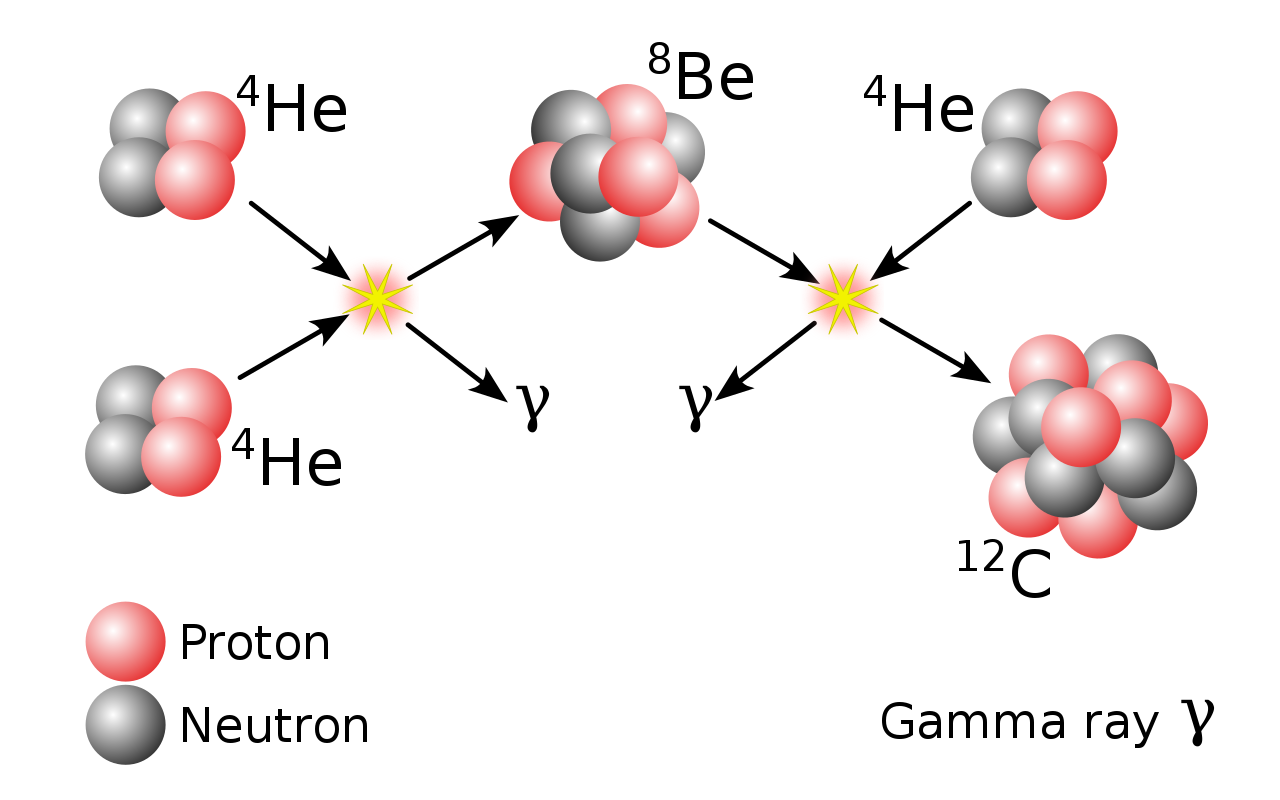
\includegraphics[width=0.5\textwidth]{graphics/sun/triple_alpha}
    \caption{Schematic of the triple-$\alpha$ process. Credit: \href{https://en.wikipedia.org/wiki/Triple-alpha_process}{Borb via English Wikipedia}.}
    \label{fig:sun:triple_alpha_process}
\end{figure}
The nuclear energy generation rate in W\,kg$^{-1}$ of the triple-$\alpha$ process, as described in \citet{carroll17} (equation (10.62) on page 312) is given as
\begin{equation}
    \epsilon_{3\alpha} = 50.9 \rho^{2} Y^{3} T_8^{-3} f_{3\alpha} \exp\left(-44.027 T_8^{-1}\right). \label{eqn:sun:triple_alpha_energy_generation}
\end{equation}
Here, $f_{3\alpha}$ is the screening factor for the triple-$\alpha$ process. Once enough carbon is produced, it becomes possible to capture another \ex{4}He on \ex{12}C, thus producing \ex{16}O in the reaction
\begin{equation}
    {^{12}}\mathrm{C} + {^4}\mathrm{He} \longrightarrow {^{16}}\mathrm{O} + \gamma.
\end{equation}

The energy release from fusing three \ex{4}He to \ex{12}C is 7.367\,MeV. While regularly, this additional energy would result in an expansion of the star, which would thus cool down and go into hydrostatic equilibrium again, the pressure does not rise in a degenerate gas. Thus, the temperature keeps rising, resulting in a vast acceleration of the triple-$\alpha$ process. This positive feedback loop results in a thermonuclear runaway, which ultimately ends in the so-called helium flash. The energy released during this helium flash does however not result in a stellar explosion but is rather used up in order to lift the degeneracy of the matter in the core, which subsequently yields a rapid expansion of the core. This expansion leads to a cooling in the hydrogen burning shell around the core, which has up to now been the sole supporter of the luminosity of the star. Thus, the Sun's luminosity drops significantly and it enters the horizontal branch on which it quietly burns helium in the core and hydrogen in a shell surrounding the core via the CNO cycle. This burning stage lasts for about 0.1\,Ga.

\paragraph{The \acl{agb}}
Once the helium in the core is exhausted, the Sun will have CO core in the center. The Sun will contract again until helium burning in a shell around the core starts. At the same time, hydrogen will be burning further out. The two areas are separated by an intershell region consisting mainly of helium. During this phase the Sun is on the \ac{eagb}. The \ac{agb} is named in this way since it asymptotically almost merges with the \ac{rgb}. The expanding and cooling star leads the convective envelope to again penetrate deeper, thus initiating the second dredge up. 

\paragraph{The \acl{tpagb}}
During the Sun's ascent of the \ac{agb}, helium burning becomes thermally unstable and the hydrogen and helium shells start burning alternatively. 
About 90\% of the time the hydrogen shell is burning, creating helium which subsequently increases the mass of helium and thus the temperature and pressure at the bottom of the intershell. At some point the temperature is high enough again to suddenly ignite helium burning at the bottom of the intershell, resulting in a thermal pulse. The Sun has now reached the \ac{tpagb} phase. 
The radius of the Sun varies by a factor of around four during this time and at its maximum radius can reach the Earth's orbit. Several of these thermal pulses will repeat at time intervals of around $10^5$\,a. Strong stellar winds during this period result in the Sun loosing a significant amount of mass. After about 20\,Ma in total, the Sun leaves the \ac{agb} branch.

\paragraph{Planetary nebula and white dwarf formation}
\begin{figure}[tb]
    \centering
    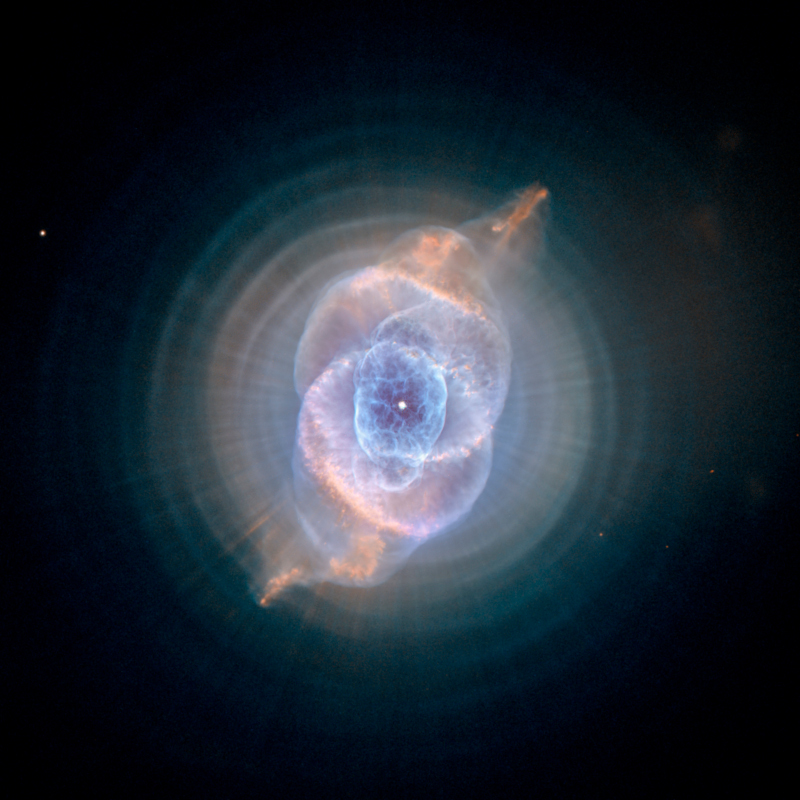
\includegraphics[width=0.6\textwidth]{graphics/sun/catseye_nebula}
    \caption{The Catseye Nebula -- a planetary nebula -- photographed with the Hubble space telescope. Credit: NASA, ESA, HEIC, and The Hubble Heritage Team (STScI / (AURA).}
    \label{fig:sun:catseye_nebula}
\end{figure}
As strong stellar winds continue, the Sun will lose enough mass to start loosing its hydrogen envelope. This exposes deeper and hotter layers, thus moving the star to the left in the \ac{hrd}. Once this surface temperature is high enough it will ionize the surrounding ejecta material via \ac{uv} radiation, making the material fluoresce brightly.
Figure~\ref{fig:sun:catseye_nebula} shows a Hubble image of the Catseye Nebula as an example of a \ac{pn}.

With ultimately all the hydrogen gone, the Sun itself will further contract until an electron degenerate CO \ac{wd} is left behind. At this point it weighs about half of its original mass. The gravitational force will be opposed by the degeneracy pressure. The \ac{wd} will continue to radiate heat away into space and thus slowly cool.


\section{The Death of More Massive Stars}

Intermediate mass stars ($2\,M_\odot < M \lesssim 8\,M_\odot$) will undergo a similar evolution to the one discussed for the Sun. During the \ac{tpagb} phase though, these stars will undergo multiple, so-called \ac{tdu} events. These events mix material from the intershell with the envelope. As we will see later, the \ac{sproc} takes place in the helium intershell. Thus, these \ac{tdu} events mix freshly nucleosynthesized material from the helium intershell into the convective envelope. Since the envelope gets ultimately ejected into space by stellar winds, \ac{sproc} material is effectively recycled into the Milky Way.

Stars more massive than $5\,M_\odot \lesssim M \lesssim 8\,M_\odot$ furthermore can successfully burn carbon further. The reactions that take place for carbon burning are the following:
\begin{equation}
    {^{12}}\mathrm{C} + {^{12}}\mathrm{C} \longrightarrow 
    \begin{cases}
        {^{16}}\mathrm{O} + 2\,{^4}\mathrm{He} \quad &(*)\\
        {^{20}}\mathrm{Ne} + {^4}\mathrm{He}\\
        {^{23}}\mathrm{Na} + p^+\\
        {^{23}}\mathrm{Mg} + n \quad &(*)\\
        {^{24}}\mathrm{Mg} + \gamma
    \end{cases}
    \label{eqn:sun:carbon_burning_reactions}
\end{equation}
Note that reactions labeled with (*) in fact consume energy and do not produce any. This behavior is however enabled by the high temperatures present during CO burning. Instead of a CO \ac{wd}, stars in this mass range leave behind a ONe \ac{wd}

Stars more massive than $8\,M_\odot$ undergo further burning reactions and end up in their final state as either neutron stars or black holes. These massive stars -- at least some -- are also expected to explode as \acp{sn}. We will discuss their fate further in the next chapter.


\section{Stellar Lifetimes}

While the quiescent burning of the Sun takes place over around 10\,Ga, subsequent burning phases are exponentially faster. The total life of the Sun is thus defined by the quiescent burning phase. This can be generalized to other stars. If the mass of a star increases, the central pressure and temperature will necessarily go up as can be seen in equations~\eqref{eqn:star_formation:central_pressure} and~\eqref{eqn:star_formation:central_temperature}, respectively. Thus, the nuclear fuel will burn faster resulting in a higher luminosity of the star. From observations of main sequence stars, an empirical mass-luminosity relation can be determined approximately as
\begin{equation}
    L = L_\odot \left(\frac{M}{M_\odot}\right)^{3.5}. \label{eqn:sun:mass_luminosity_relation}
\end{equation}

The lifetime of a star is proportional to its mass divided by its luminosity, since the mass is proportional to the amount of fuel (see also, equation~\ref{eqn:star_formation:nuclear_lifetime}). We can therefore roughly estimate the lifetime dependency in comparison to the solar lifetime with respect to a star's mass. The dependency yields
\begin{equation}
    t_\mathrm{nuc}(M) \approx t_{\odot\mathrm{,total}} \left(\frac{M_\odot}{M}\right)^{2.5}. \label{eqn:sun:stellar_lifetime_estimate}
\end{equation}
This equation should solely be used for back-of-the-envelope-type calculations, however, it helps to understand the fact that more massive stars die faster. Detailed determinations of the stellar lifetimes require adequate models that include the energy generation equations, e.g., equations~\eqref{eqn:sun:energy_generation_pp-chain} and~\eqref{eqn:sun:energy_generation_cno_cycle}, as well as an accurate thermodynamic model of the inside of a star.

\section{Reading}

In this chapter we have in detail discussed the inner workings of the Sun. The reading chosen to supplement our theoretical understanding of the Sun discusses the experimental work that went into actually observing the quiescent burning using neutrino detectors.

Please read \citet{davis55} and \citet{bahcall76}. We will briefly discuss \citet{davis55} and these pioneering measurements and then focus on \citet{bahcall76}. The following points might help to guide the reading:
\begin{itemize}
    \item What is the general understanding of neutino research in 1955? How does this influence the hypothesis of \citet{davis55}?
    \item Discuss the experimental setup of \citet{davis55}. It might help to make a drawing of the setup to the best of your understanding. Split the setup up into two parts, (1) how to get \ex{37}Ar out of the tank and (2) how it is subsequently detected.
    \item What are the (stunning) conclusions of \citet{davis55}?
    \item How has the knowledge of neutrinos changed in between \citet{davis55} and \citet{bahcall76}?
    \item What neutrinos can be detected with the experiment of \citet{bahcall76}? Which reactions do these neutrinos originate from? Put your findings into context of Figure~\ref{fig:sun:pp-chain}.
    \item What is different in the experimental setup disucssed in \citet{bahcall76} compared to \citet{davis55}?
    \item Discuss why the experiment described in \citet{bahcall76} was performed underground? Compare the Homestake mine to other underground laboratories. Was the shielding of the mountain enough to achieve the required sensitivity?
    \item How did the experimentalists ensure that their result is correct?
    \item What solar processes can be excluded from these measurements? Where lies the solar neutrino problem?
    \item What alternative explanations are given by \citet{bahcall76} that might solve the solar neutrino problem?
    \item Who won in the end, the astronomers or the physicists? What implication did this finding have -- for the world and for Ray Davis?
\end{itemize}
%!TEX root = origin_elements_lecture_notes.tex

\chapter{The Fate of Massive Stars}\label{ch:massive_stars}
Compared to stars with masses of up to $\sim 8\,M_\odot$, massive stars undergo different burning phases that significantly differ from what was discussed in Chapter~\ref{ch:sun}. Here, we will first discuss observations that led to the discovery and classification of massive stars and their properties. We will then discuss in more details how massive stars evolve and ultimately die before discussing massive star contributions of freshly nucleosynthesized material to the solar nebula 4.5\,Ga ago.

\section{Observations}

\subsection{Wolf-Rayet Stars} In 1867, the French astronomers Charles Wolf and Georges Rayet observed three stars in the Cygnus constellation that emitted unusually broad emission instead of the typical absorption lines. Along with these emission lines, these now so-called \ac{wr} stars are also very hot with effective temperatures of $(25 - 100)\times 10^{3}$\,K. \ac{wr} stars also show very high mass losses in excess of $10^{-5}\,M_\odot$\,a$^{-1}$ with wind speeds ranging from 800\,km\,s$^{-1}$ to 3000\,km\,s$^{-1}$ and many are rapidly rotating with typical equatorial speeds of around 300\,km\,s$^{-1}$. Figure~\ref{fig:massive_stars:wr124} shows an image of a \ac{wr} star, namely star WR124. 

In addition, the spectra different \ac{wr} show different compositions. The spectra of WN stars are dominated by emission lines of helium and nitrogen. For WC stars, helium and carbon dominate the spectra while nitrogen and hydrogen are absent. Finally, WO stars, which are rarer than the other two types, contain prominent oxygen lines and have some contribution to their spectra from highly ionized species. These different features are direct consequences of the mass loss of these massive stars.


\subsection{Supernovae}
\begin{figure}[tb]
    \centering
    \begin{subfigure}{0.495\textwidth}
        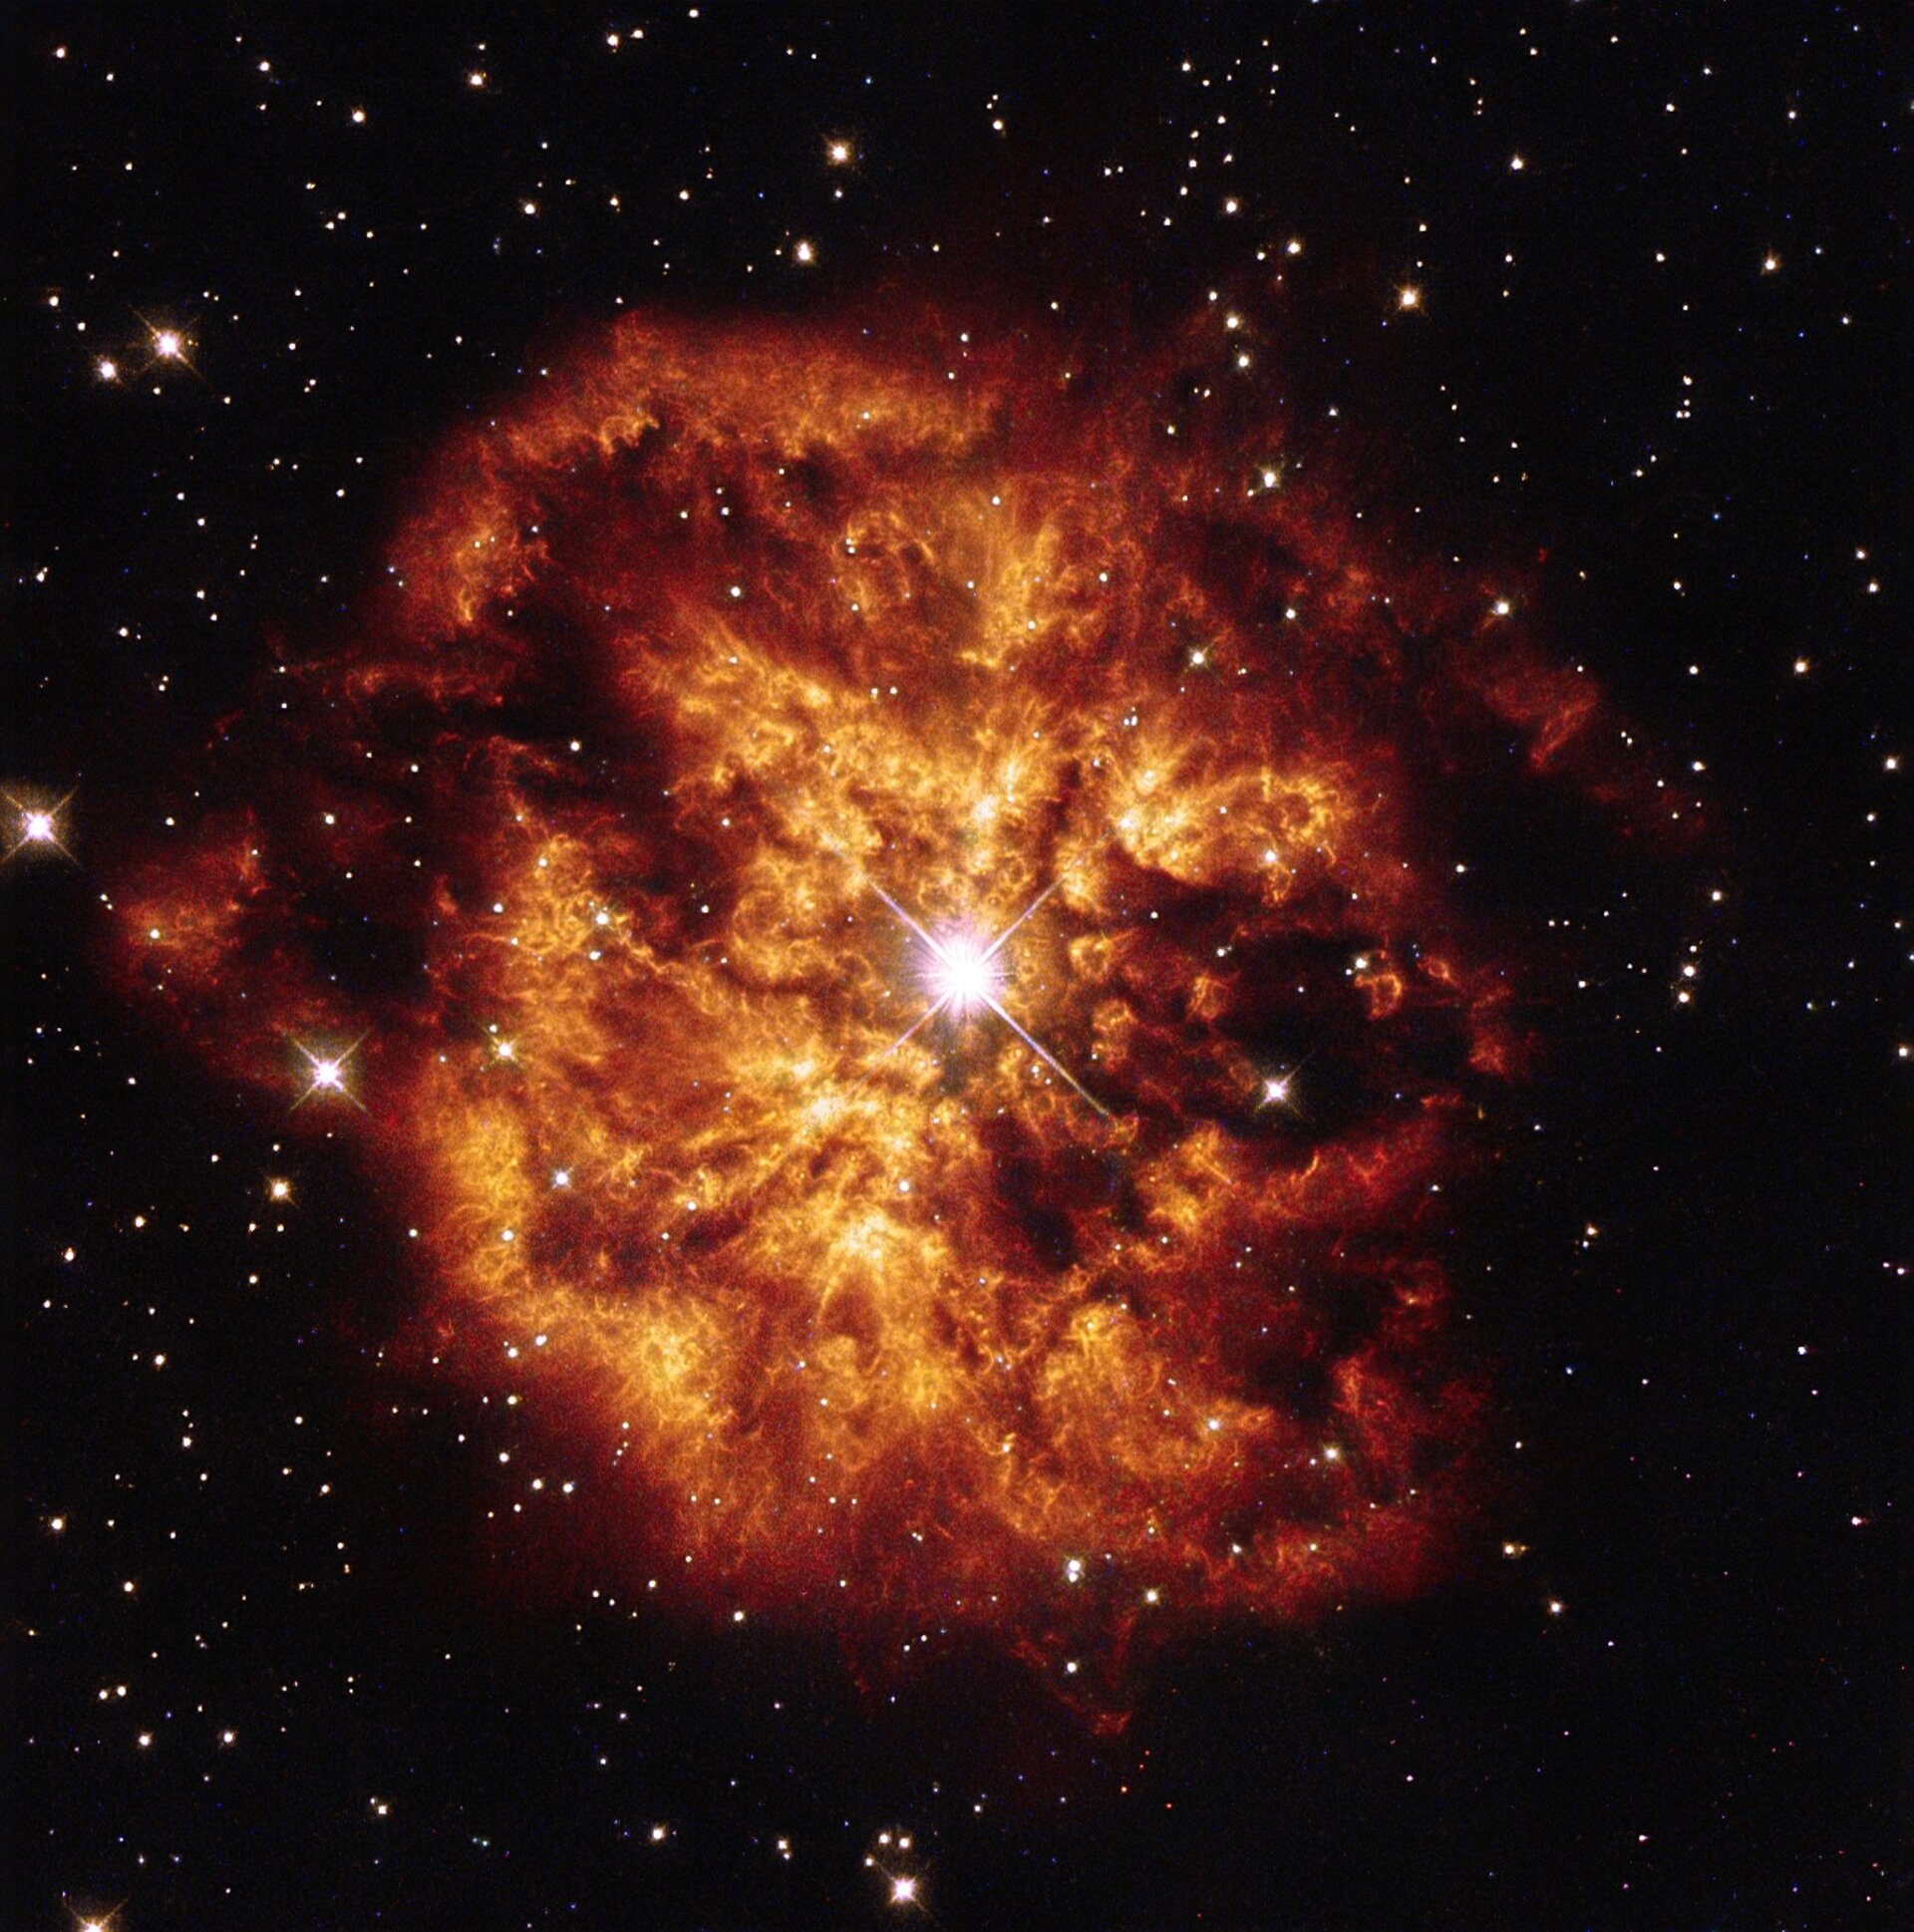
\includegraphics[width=\textwidth]{graphics/massive_stars/wr124}
        \caption{Wolf-Rayet star WR124. Credit: ESA, Hubble \& NASA.}
        \label{fig:massive_stars:wr124}
    \end{subfigure}
    \begin{subfigure}{0.495\textwidth}
        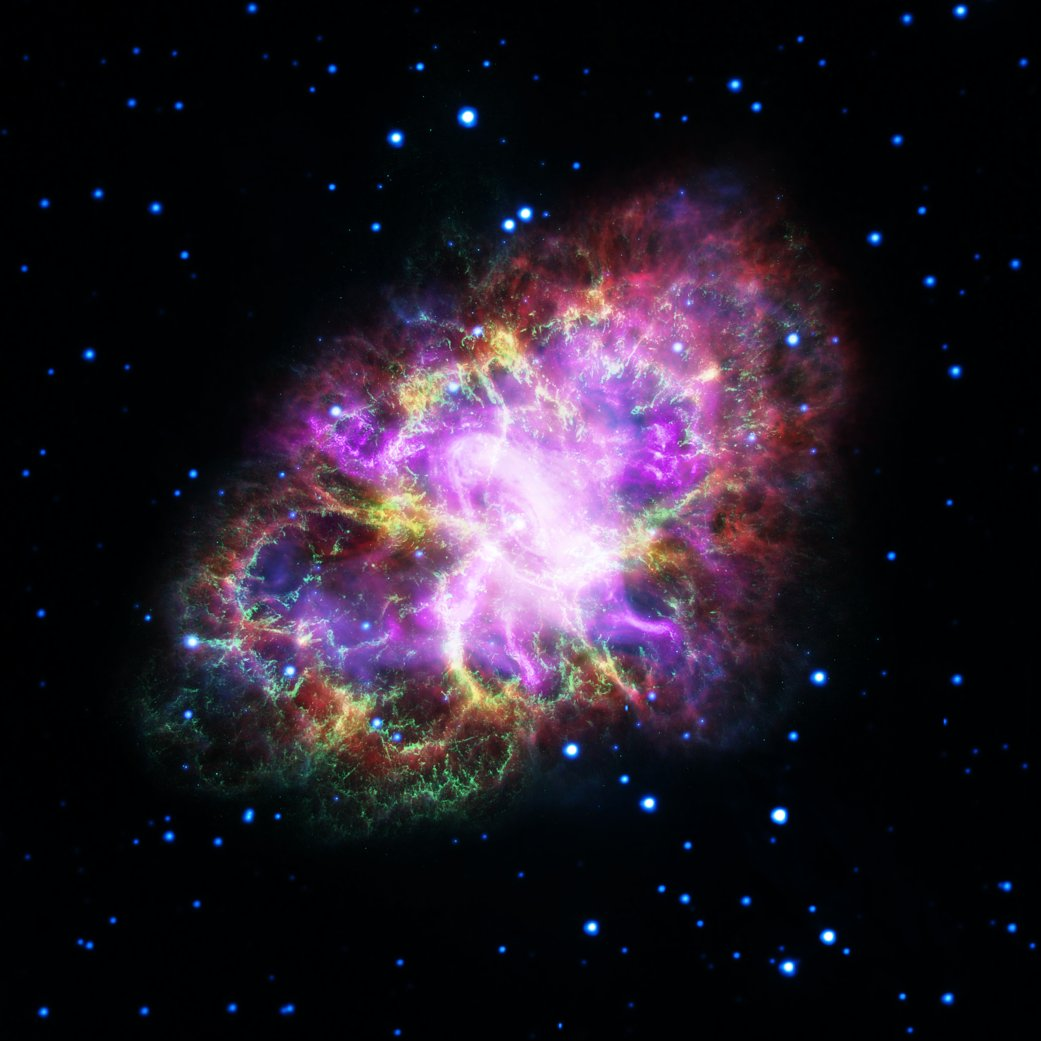
\includegraphics[width=\textwidth]{graphics/massive_stars/crab_nebula}
        \caption{The crab nebula. Credit: NASA, ESA, NRAO/AUI/NSF \& G. Dubner.}
        \label{fig:massive_stars:crab_nebula}
    \end{subfigure}
    \caption{Massive stars at different evolutionary times.}
    \label{fig:massive_stars:massive_stars_figure}
\end{figure}
Throughout the written history of humanity, new stars have been observed all over the world. Based on various writings from astrologers in China, Egypt, Europe, Iraq, and Japan, a star appeared in the Taurus constellation around April 30, 1006, and faded from view about one year later. Modern telescopes allowed the detection of the remnant of this new star which can today still be detected as the crab nebula. This \ac{sn} remnant is shown in Figure~\ref{fig:massive_stars:crab_nebula}. While the last \ac{sn} to occur in the Milky Way was in 1604, an event that was reported by Tycho Brahe and Johannes Kepler, supernovae in other galaxies can also be observed with modern telescopes. 

One event that deserves special mentioning is \ac{sn} 1987A. Since multiple \acp{sn} are recorded every year, they are now cataloged with the year and a subsequent letter. \ac{sn} 1987A was discovered on February 24, 1987, in the large Magellanic cloud, a satellite galaxy of the Milky Way. It was quickly determined that the progenitor of this event was a blue supergiant star. The proximity of the event further allowed it to be studied with various techniques. For example, the light curve could be measured and analyzed in detail. Furthermore, a total of 20 neutrinos from \ac{sn} 1987A were detected in Japan and the US. These neutrinos arrived three hours before the photons of the event reached Earth, thus significantly constraining the upper limit of the neutrino mass.

\begin{figure}[tb]
    \centering
    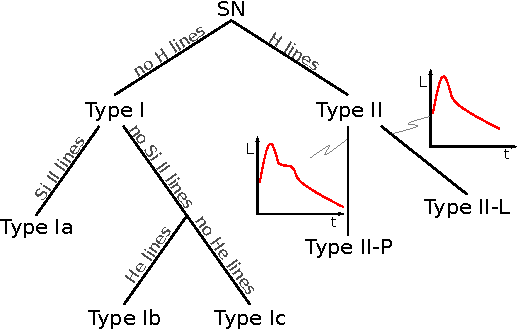
\includegraphics[width=0.6\textwidth]{graphics/massive_stars/sn_classification}
    \caption{Classifaction of \acp{sn} based on their spectra at maximum light and their light curves.}
    \label{fig:massive_stars:sne_classification}
\end{figure}
Figure~\ref{fig:massive_stars:sne_classification} shows a schematic on how supernovae are classified based on observational properties. Note that this classification is purely based on (1) the spectral lines present and (2) the shape of the light curve. If no hydrogen lines are present in \ac{sn} it is classified as a type I \acl{sn}, otherwise as an \ac{snii}. Type I \acp{sn} are further subdivided into three categories: \ac{snia} contain no singly-ionized silicon (Si II) lines while \ac{snib} and \ac{snic} do. The former in additional show helium lines while the latter do not. If the spectrum of the \ac{sn} shows hydrogen lines, it is by definition a \ac{snii}. Further subdivisions are based on the light curve emitted by the event. Figure~\ref{fig:massive_stars:sne_classification} shows examples of light curves. If it contains a plateau it is called a \ac{sniip}, otherwise an \ac{sniil}. We will see later why the different types show the specific features mentioned in Figure~\ref{fig:massive_stars:sne_classification}.



\section{The Evolution of Massive Stars}

Before we discuss in detail how \acp{sn} explode, let us discuss the individual burning phases that stars with masses $M \gtrsim 8\,M_\odot$ undergo.
\begin{figure}[tb]
    \centering
    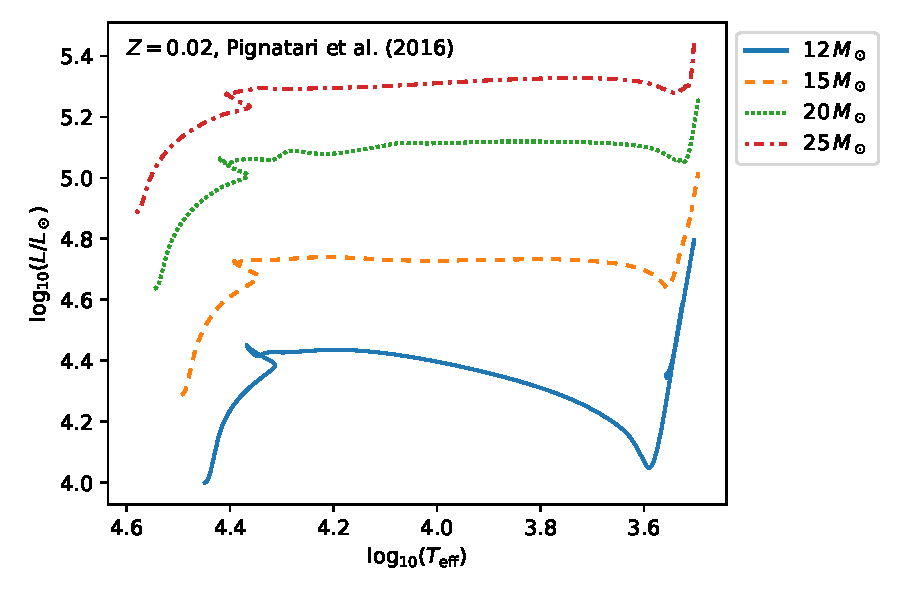
\includegraphics[width=0.8\textwidth]{graphics/massive_stars/hrd_massive_stars}
    \caption{Evolution of various massive stars in the \ac{hrd} after they left the main sequence. Data from \citet{pignatari16}.}
    \label{fig:massive_stars:hrds_pignatari_nugrid_set1.2}
\end{figure}
Figure~\ref{fig:massive_stars:hrds_pignatari_nugrid_set1.2} shows the evolution of massive stars in the \ac{hrd}. Stellar models are for a metallicity of $Z=0.02$ and are taken from \citet{pignatari16}. The paths of the stars on the \ac{hrd} start when they leave the main sequence. While the evolution of the shown stars all look fairly similar, they are vastly different from the fate that lower-mass stars undergo. Here, the $25\,M_\odot$ star is discussed as an example. Such a star lives for around 9\,Ma \citep{meynet03}. Even though massive stars are much rarer than low-mass stars, the short lifetime results in these stars rapidly recycling freshly nucleosynthesized material back into the Milky Way, thus enriching it in metallicity. Recycling also takes place prior to the supernova, since stellar winds can drive parts of the atmosphere out into space. 

\begin{table}[b]\label{codebox:nugrid}
\codebox{NuGrid Collaboration and Data Access}{The \href{https://nugrid.github.io/}{Nucleosynthesis Grid (NuGrid) international collaboration} develops and maintains tools for large-scale nucleosynthesis post-processing simulations and to analyze stellar evolution models created with MESA. Especially interesting is that all stellar models and postprocessing data is released publicly. NuGrid maintains a public JupyterLab server that can be accessed by anybody to explore stars. This systems has also been used to create Figure~\ref{fig:massive_stars:hrds_pignatari_nugrid_set1.2} and is available on the \href{https://astrohub.uvic.ca/}{University of Victoria's AstroHub site}.}
\end{table}

\paragraph{Helium burning}
Hydrogen burning takes place for around 90\% of the star's lifetime, mainly via the CNO cycle (see Figure~\ref{fig:sun:energy_generation_hydrogen_fusion}). When the core is exhausted, hydrogen burning continues in a shell. The core starts contracting until the temperature is high enough to ignite helium burning, at which point the star significantly increases in size and becomes a supergiant. Examples of such stars are Rigel or Betelgeuse, a blue and red supergiant, respectively, in the constellation Orion. In fact, on a clear night in winter you can easily identify these two stars by eye due to their color. Helium burning in the core lasts for less than 1\,Ma and during this time, neutron captures can lead to the formation of some heavy nuclei with $A>60$. This is the so-called weak \ac{sproc} and is responsible for the \ac{sproc} isotopes between nickel and strontium. Details on the \ac{sproc} will be discussed in Chapter~\ref{ch:s-process}. 

\paragraph{Carbon, neon, and oxygen burning}
The ashes left behind after helium burning mainly consist of \ex{12}C and \ex{16}O. Of the possible reactions, carbon burning has the lowest threshold and starts first. The main reactions are as already seen in~\eqref{eqn:sun:carbon_burning_reactions}.
The main leftovers after this reaction are \ex{16}O and \ex{20}Ne.

After carbon burning, the star contracts once more and the temperature and density rise to a point at which photodisintegration reactions become important. This in fact first leads to the reaction
\begin{equation}
    {^{20}}\mathrm{Ne} + \gamma \longrightarrow {^{16}}\mathrm{O} + \alpha,
\end{equation}
which is endothermic and consumes 4.73\,MeV of energy. Note that $\alpha$ is equivalent to a \ex{4}He nucleus. Subsequent, main exothermic reactions that take place during neon burning are
\begin{align}
    {^{20}}\mathrm{Ne} + \alpha &\longrightarrow {^{24}}\mathrm{Mg} + \gamma \\
    {^{24}}\mathrm{Mg} + \alpha &\longrightarrow {^{28}}\mathrm{Si} + \gamma \\
    {^{23}}\mathrm{Na} + \alpha &\longrightarrow {^{26}}\mathrm{Mg} + p \\
    {^{26}}\mathrm{Mg} + \alpha &\longrightarrow {^{29}}\mathrm{Si} + n.
\end{align}
Here, $p$ stands for an individual proton. The overarching production taking place during neon burning is
\begin{equation}
    {^{20}}\mathrm{Ne} + {^{20}}\mathrm{Ne} \longrightarrow {^{16}}\mathrm{O} + {^{24}}\mathrm{Mg}
\end{equation}
and releases 4.6\,MeV of energy.

After neon has efficiently been destroyed, \ex{16}O, \ex{24}Mg, and \ex{28}Si are the most abundant nuclei in the star. Again the core contracts and heats up until oxygen burning starts. The important reactions are:
\begin{equation}
{^{16}}\mathrm{O} + {^{16}}\mathrm{O} \longrightarrow 
    \begin{cases}
        {^{24}}\mathrm{Mg} + 2\,{^4}\mathrm{He} \quad & (*)\\
        {^{28}}\mathrm{Si} + {^4}\mathrm{He}\\
        {^{30}}\mathrm{P} + d \quad & (*)\\
        {^{31}}\mathrm{P} + p\\
        {^{30}}\mathrm{S} + 2\,p\\
        {^{31}}\mathrm{S} + n\\
        {^{32}}\mathrm{S} + \gamma
    \end{cases}
    \label{eqn:massive_stars:oxygen_burning_reactions}
\end{equation}
Here $d$ stands for a deuterium nucleus. 

\paragraph{Silicon burning}
At the end of oxygen burning, the most abundant nuclei in the star are \ex{28}Si and \ex{32}S. The core again contracts, however, reactions combining \ex{28}Si and \ex{32}S directly are too unlikely to occur due to coulomb barrier considerations. Instead, the higher temperatures allow photodisintegration of some nuclei to form protons, neutrons, and \ex{4}He particles. These can subsequently be caught on \ex{28}Si and \ex{32}S to form heavier, more tightly bound nuclei. Silicon burning reactions take place on a timescale of about 1\,d and at temperatures in the range of $3-4$\,GK.

\begin{figure}[tb]
    \centering
    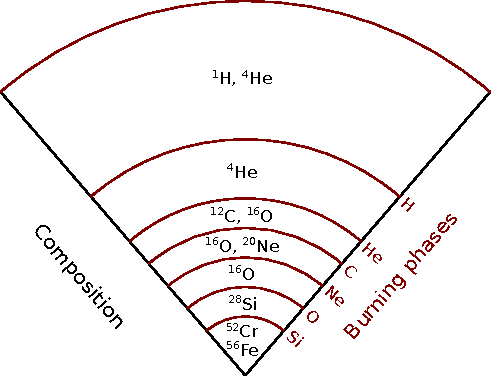
\includegraphics[width=0.6\textwidth]{graphics/massive_stars/pre-supernova}
    \caption{Schematic structure of the pre-supernova star, not to scale. In black inidcated are the most abundant isotopes in each shell \citep{limongi2000}. Inidcated in red are the nuclear burning shells.}
    \label{fig:massive_stars:pre-supernova_structure_schematic}
\end{figure}
Figure~\ref{fig:massive_stars:pre-supernova_structure_schematic} shows a schematic of the star's composition at towards the end of the silicon burning. The inner core consists mostly of \ex{56}Fe and \ex{52}Cr. This onion like structure has lighter elements towards the surface and all composition changes are separated from each other by respective burning shells. Note that ashes of these nuclear fires accumulate at the bottom of each shell and get added to the inner parts, e.g., silicon burning is constantly adding ashes to the core.

\infobox{Coulomb barrier}{Since atomic nuclei are positively charged, they repell each other. The Coulomb barrier describes the energy that needs to be overcome in order for two nuclei to interact. With the nuclei at distance $r$ and charges $q_1$ and $q_2$, the Coulomb energy can be written as
\begin{equation}
    E_\mathrm{coul} = k_C \frac{q_1 q_2}{r}. \label{eqn:massive_stars:coulomb_energy}
\end{equation}
Here, $k_C=8.9876\times10^{9}$\,N\,m$^{2}$\,C$^{-2}$ is Coulomb's constant. 

\href{https://en.wikipedia.org/wiki/Quantum_tunnelling}{Quantum tunneling} enables two nuclei to fuse even below this energy. The conditions under which tunneling is allowed are found in the so-called \href{https://en.wikipedia.org/wiki/Gamow_factor}{Gamow window.}}

\paragraph{Nuclear statistical equilibrium}
At the end of silicon burning, once most of the \ex{28}Si has been processed further, the temperature and density in the star steadily increases until the point is reached at which production and destruction processes of nuclei come into equilibrium. Once every nuclei in the network from protons, neutrons, and \ex{4}He up to the iron peak nuclei is equally likely to be produced and destroyed, \ac{nse} is achieved. This will soon become more important, namely once the stellar explosion sets in.


\section{Core-Collapse Supernovae}

Depending on the initial mass of the star, various fates can yield a supernova explosion. In our example $25\,M_\odot$ case, the degenerate iron core of the pre-supernova (Figure~\ref{fig:massive_stars:pre-supernova_structure_schematic}) is constantly being fed with ashes from the silicon burning shell around it. Once the core mass reaches the \href{https://en.wikipedia.org/wiki/Chandrasekhar_limit}{Chandrasekhar limit} of roughly $1.4\,M_\odot$, the degeneracy pressure can no longer counteract the gravitational force and thus the core collapses freely with a speed of about $0.25c$. The core collapses to a density of $\rho\approx10^{14}$\,g\,cm$^{-3}$, which is similar to the density of the nuclei themselves. At this point, the strong force, which is usually attractive, becomes repulsive. Overshooting in nuclear density, the inner core of the star now acts as a stiff spring, which results in the creation of a shock wave and a bounce back that now travels outwards and passes the material form outer shells that is gravitationally collapsing onto the core. 

The outward moving shock leads to photodisintegrations of iron-peak nuclei, which in return removes energy from the shock wave itself. Further energy is lost by neutrino emission, which ultimately results in the shock stalling when it has reached the outer edge of the core around 1\,s after core collapse (10\,ms after the bounce). Infalling material now accretes onto the shock wave.

It is not yet clear how exactly the shock wave starts up again. One possibility is that a neutrinosphere builds up in the core from the processes of photodisintegration and electron capture. The area where the shock stalled is now so dense that neutrinos cannot easily penetrate it. Thus, these neutrinos are estimated to deposit around 5\% of their total energy in the matter just behind the shock. The heat deposited in this area allows the shock to be revived and continue its path towards the stellar surface. If this process does not occur, the material will fall back onto the core and ultimately lead to the formation of a neutron star or black hole, and no stellar explosion occurs. It is in fact still unclear what stars explode (mass, metallicity) and how exactly. Large supercomputers are being used to track the evolution of supernovae, however, due to the timescales and complexity of the problem, detailed 3D simulations progress slowly.\footnote{Some links to go down the rabbit hole: \href{https://ccsweb.lanl.gov/astro/index.html}{Center for Theoretical Astrophysics at Los Alamos National Laboratory}, \href{https://www.scidac.gov/}{Scientific Discovery through Advanced Computing (SciDAC)}, \href{https://2sn.org/}{Alex Heger}}

It is thought that \acp{snib}, \acp{snic}, and \acp{snii} are all result from core-collapse of a massive star. Differences originate from the original composition of the star, which also influences the exact mechanism of the supernova trigger.

\subsection{Explosive burning and freeze-out}

We have established the conditions for nuclear statistical equilibrium above, which is achieved at high enough temperatures. The shock wave, however, heats material as it travels outwards and thus induces further burning of these fuels in a process called explosive burning. As the shock moves outwards, the star expands and cools, thus material on the inside experiences a rapid decrease in temperature. 

Nucleosynthesis reactions taking place under these circumstances are highly dependent on the densities of free, light particles such as protons, neutrons, and $\alpha$-particles. If the fraction of available \ex{4}He nuclei is small, $\alpha$-poor freeze out takes place, resulting in the production of mostly iron peak elements such as \ex{56}Ni, \ex{54}Fe, and \ex{56}Fe. On the other hand, if many free $\alpha$-particles are available, $\alpha$-rich freeze out takes place, which creates elements along the chain of multiples of $\alpha$-particles, e.g., 
\begin{equation}
    \alpha (2\alpha, \gamma) ^{12}\mathrm{C} (\alpha, \gamma) ^{16}\mathrm{O} \quad \dots \quad ^{52}\mathrm{Fe} (\alpha, \gamma) ^{56}\mathrm{Ni}.
\end{equation}

\begin{figure}[tb]
    \centering
    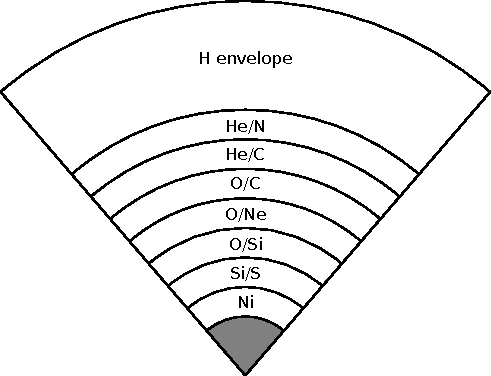
\includegraphics[width=0.6\textwidth]{graphics/massive_stars/post-supernova}
    \caption{Schematic structure of the post-supernova star, not to scale. Given are the 1-2 most abundant elements in every zone, which give the zone its name \citep{meyer95}. The gray area represents the material left behind in the explosion, either a neutron star or a black hole.}
    \label{fig:massive_stars:post-supernova_structure_schematic}
\end{figure}
Figure~\ref{fig:massive_stars:post-supernova_structure_schematic} shows the composition of the ejecta from a star post-supernova. Labels represent the most abundant element(s) for a given layer. These layers are generally named after the two most abundant elements present in them \citep{meyer95}.

\subsection{Fall-back}

Depending on the initial conditions of a star, e.g., mass and metallicity, either a neutron star or a black hole are left behind after the supernova explosions. Some of the material that first expands will get pulled back and fall onto the remnant. How much mass exactly falls back \citep[e.g.,][]{heger03} will define the amount of material that gets recycled back into the galaxy and thus contributes to its enrichment in metals.



\subsection{Neutrinos and Supernova Luminosity}

Assuming that the shock wave propagates through the star as discussed above, the total kinetic energy released in a supernova explosion is around $10^{44}$\,J. This is equivalent to roughly 1\% of the total energy released by neutrinos.

In both scenarios above, freeze-out conditions result in the production of \ex{56}Ni, a radioactive isotope of nickel. It decays to \ex{56}Co with a half-life of around 6\,d, which then furthermore decays to \ex{56}Fe with a half-life of 77.2\,d. Energy from the $\gamma$-rays that are emitted by the decaying nuclei is subsequently deposited into the thick, expanding envelope that moves away from the star. This envelope then radiates the energy in the form of visible light. The light curves of supernovae are thus determined by the radioactive decay taking place. The peak luminosity that is generally achieved is around $10^9\,L_\odot$, which is bright enough to outshine whole galaxies and thus explain the terminology: \acl{sn}. 

The plateau in \acp{sniip} (see inset in Figure~\ref{fig:massive_stars:sne_classification}) is likely the result of the recombination of hydrogen molecules, which emits light as the ejecta cools. Much less hydrogen is present in the envelopes of \acp{sniil}, thus no plateau in the light curve occurs.


\infobox{1\,foe}{Traditionally, the \ac{sn} community uses cgs units. The kinetic energy of a typical \ac{sn} shockwave in cgs units is around $10^{51}$\,erg. Gerald E. Brown and Hans Bethe coined the term 1\,foe, where foe stands for fifty-one erg, in order to have a more convenient way of talking about \acp{sn} explosions. Later, Steven Weinberg proposed to rename it to 1\,bethe (B). All notations are found in the literature.}



\section{Type Ia Supernovae}\label{sec:massive_stars:snia}

In contrast to core-collapse \acp{sn} described above, \ac{snia} take place in binary star systems. One remarkable property of these events is that their maximum luminosity seems to be very constant and only shows minor spread. Therefore, \acp{snia} are used as standard candles in cosmology, i.e., to determine distance to far away galaxy and to measure the Hubble constant and expansion rate of the universe. However, significant discrepancies have been found when determining the Hubble constant using \ac{snia} as standard candles and when measuring it via the \ac{cmb}.\footnote{\url{https://www.sciencenews.org/article/debate-universe-expansion-rate-hubble-constant-physics-crisis}} Recently, \citet{freedman19} used the brightness of stars on the tip of the red giant branch to determine the Hubble constant again. The result landed right in between the determination via \acp{snia} and using the \ac{cmb}. 

Aside from their effect on cosmology, \acp{snia} are also expected to contribute a significant amount of nucleosynthesized material to the Milky Way. A better understanding of their origin is thus crucial to decipher \ac{gce} as well as the cosmological implications.


\subsection{The Single-Degenerate Scenario}

The exact mechanisms behind \acp{snia} are poorly understood, however, researchers are focusing in on roughly two scenarios, both of which could occur in nature.
\begin{figure}[tb]
    \centering
    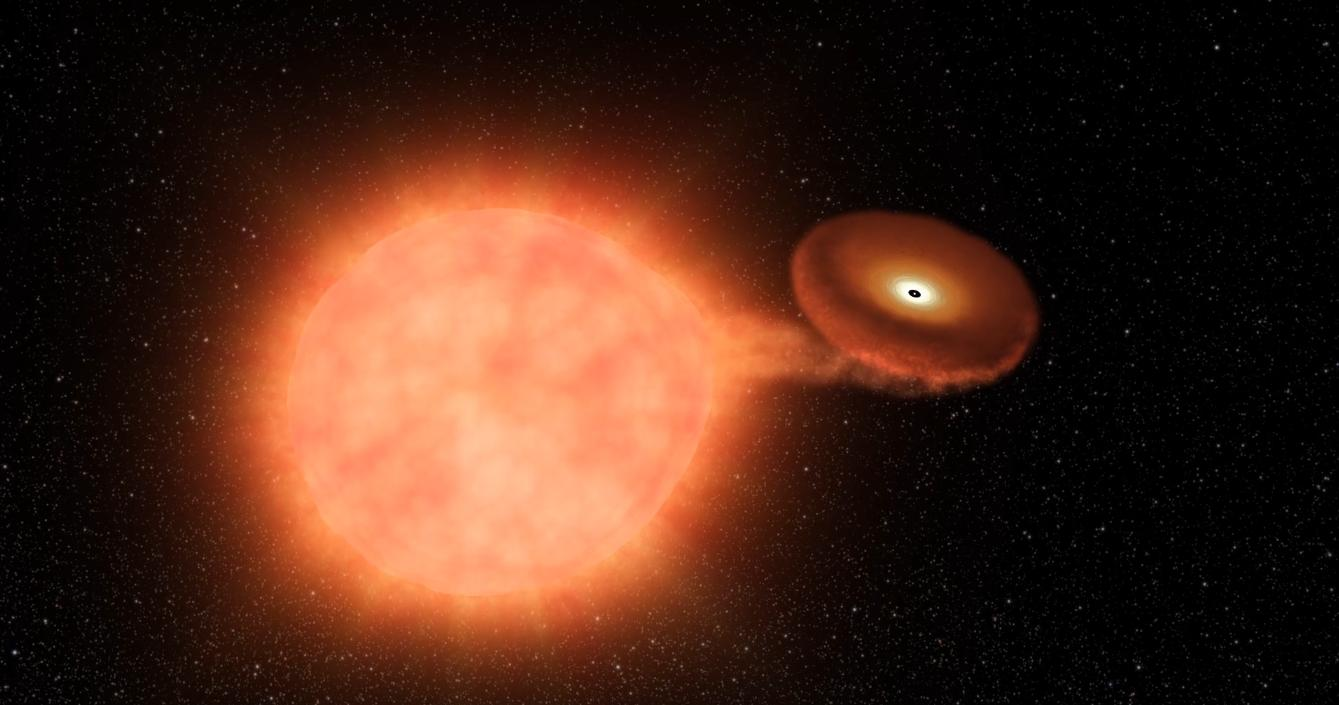
\includegraphics[width=0.75\textwidth]{graphics/massive_stars/sn-ia-artistic}
    \caption{Artistic view of the accretion that leads to a \ac{snia} explosion. Credit: NASA/JPL.}
    \label{fig:massive_stars:sn_ia_artistic}
\end{figure}
Figure~\ref{fig:massive_stars:sn_ia_artistic} shows an artistic view of the single-degenerate scenario for \ac{snia} explosions. In this scenario, a degenerate CO \ac{wd} accretes matter from a companion star at a relatively large rate of around $10^{-7}\,M_\odot\,\mathrm{a}^{-1}$. The companion star could, e.g., be a Red Giant. When the mass of the degenerate, primary star exceeds the Chandrasekhar limit ($\sim1.4\,M_\odot$), the carbon core ignites under degenerate conditions. A thermonuclear runaway occurs, which ultimately leads to the \ac{sn} explosion that completely disrupts the \ac{wd}. The companion star likely survives the explosion. During this explosion, nucleosynthesis takes place via nuclear statistical equilibrium, resulting in the production of mainly around $0.6\,M_\odot$ of \ex{56}Ni and some lighter nuclei. The amount of \ex{56}Ni is responsible for the typical and constant light curve.


\subsection{The Double-Degenerate Scenario}

In this scenario, the \ac{snia} occurs via the collision of \acp{wd}. In a close binary system, two \acp{wd} will spiral inwards because of momentum loss due to gravitational wave emission. Once close enough, the less massive star will start loosing mass to the more massive star. Once the mass of the degenerate core again reaches the Chandrasekhar limit, carbon burning ignites and proceeds similar to the single-degenerate scenario. In this case, both stars are completely disrupted leaving behind no remnant.


\subsection{Open Questions and the Cosmological ``Crisis''}

Many open questions remain with respect to \acp{snia}. It is unclear which scenario in fact leads to the formation of \acp{snia} and it could easily be the case that more than one trigger exists. Furthermore, metallicity likely has some influence on the exact explosion mechanism and on the light curve. One speculation to resolve the Hubble constant crisis is that \ac{snia} formation is different in galaxies at high redshifts compared to the near universe. This could potentially resolve the discrepancies without requiring ``new physics'' (see also Chapter~\ref{ch:bbn}). The recent measurements by \citet{freedman19} are surely a promising indication into this direction.



\section{Massive Star Contributions to the Early Solar System}

It has been shown \citep{jacobsen08} that the Solar System started with a canonical \ex{26}Al/\ex{27}Al ratio of $5\times10^{-5}$. Since \ex{26}Al is \iac{slr} with a half-life of $7.17\times10^{5}$\,a and decays to \ex{26}Mg. This \ac{slr} must have been supplied to the solar nebula shortly before the collapse of the molecular cloud and the subsequent formation of the first solids. 

\subsection{Isochron Measurements}

In order to determine the amount of \acp{slr} in meteoritic material, mineral phases with various different elemental aluminum-to-magnesium ratios are measured for their magnesium isotopic content. 
\begin{figure}[tb]
    \centering
    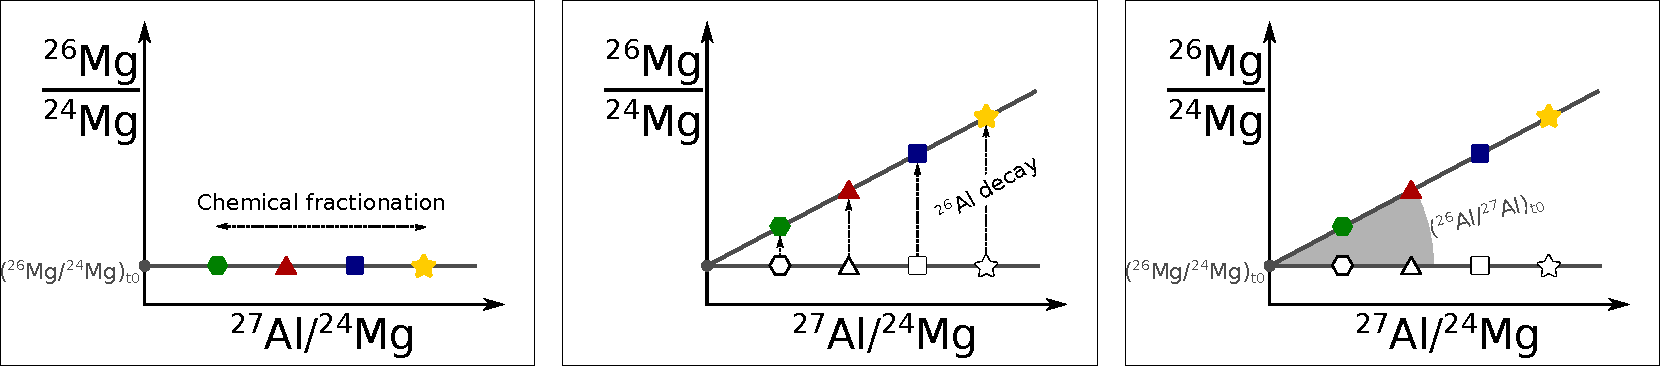
\includegraphics[width=\textwidth]{graphics/massive_stars/al26_isochron}
    \caption{Schematic representation to show how an isochron develops over time in different minerals within a given meteorite.}
    \label{fig:massive_stars:al26_isochron}
\end{figure}
Figure~\ref{fig:massive_stars:al26_isochron} shows a schematic of the formation for an isochron. Different mineral phases of a given meteorite (left) will incorporate various amounts of magnesium and aluminum according to their respective composition. If a phase incorporates live \ex{26}Al, the amount it incorporates is constant with respect to the amount of the stable \ex{27}Al. Over time, all \ex{26}Al decays, thus raising the respective \ex{26}Mg/\ex{24}Mg isotope ratio in the given phase (center panel in Figure~\ref{fig:massive_stars:al26_isochron}). Finally, when measured in a meteorite 4.567\,Ga later, measurements plotting on an isochron (right panel in Figure~\ref{fig:massive_stars:al26_isochron}) indicate a common age and can be used to derive the solids initial \ex{26}Al/\ex{27}Al ratio. Mathematically this can be expressed as
\begin{equation}
    \frac{^{26}\mathrm{Mg}}{^{24}\mathrm{Mg}} = \left(\frac{^{26}\mathrm{Al}}{^{27}\mathrm{Al}}\right)_0 \times \frac{^{27}\mathrm{Al}}{^{24}\mathrm{Mg}} + \left(\frac{^{26}\mathrm{Mg}}{^{24}\mathrm{Mg}}\right)_0.
\end{equation}
The slope of the linear correlation represents the wanted quantity; the initial \ex{26}Al/\ex{27}Al composition.


\subsection{The Iron-60 Controversy}

Using various mineral phases and in situ measurements of meteoritic phases, the initial composition of \ex{60}Fe/\ex{56}Fe was determined by various authors to be on the order of $10^{-7}$ to $10^{-6}$ \citep[e.g.,][]{mishra14,telus18}. This high abundance would be consistent with a co-production of \ex{26}Al and \ex{60}Fe in a \ac{sn}, which could also have triggered the collapse of the Solar System's molecular cloud.

On the other hand, bulk measurements of meteorites showed an initial \ex{60}Fe/\ex{56}Fe ratio for the early Solar System of $(1.01 \pm 0.27)\times10^{-8}$ \citep{tang12,tang15}. This \ex{60}Fe value could easily be consistent with the galactic background. More importantly it prohibits \acp{sn} from being the main contributor of \ex{26}Al. The longer life-time of \ex{60}Fe ($t_{\nicefrac{1}{2}} = 2.62 \times 10^{6}$\,a) with respect to \ex{26}Al only allows the \ex{26}Al/\ex{60}Fe ratio to decrease over time. Even within the uncertainties in the nucleosynthesis calculations, \acp{sn} would contribute too much \ex{60}Fe is supplying all \ex{26}Al \citep{jones19}. The origin of \ex{26}Al is thus likely a different stellar source, a likely candidate being nucleosynthesis in stellar winds of a \ac{wr} star \citep{dwarkadas17}.

The solution to the issue of measurement discrepancies likely originates in the data processing of the in situ measurements that determined the high \ex{60}Fe/\ex{56}Fe values. \citet{trappitsch18} re-measured one sample and found no effects due to in situ decay of \ex{60}Fe. These measurements and evaluations pointed into the direction of in situ data evaluation issues. Further work is currently ongoing and will likely solve the \ex{60}Fe controversy; no proof has so far been brought forward that the amount of \ex{60}Fe is different from what is expected from galactic background.


\section{Reading}

Please read \citet{fry15}. You may skim through Sections~3 and~4, however make sure you understand the ingredients for equation~(1). For discussion, focus on the big picture of what the authors are trying to address. Furthermore, many different fields play a role here. Try to decipher the connections and difficulties that the different researchers bump into when contributing to the big picture. The following points might help with the reading:

\begin{itemize}
    \item What isotope signatures have been found for a nearby, recent \ac{sn} explosion and where were these signals detected?
    \item How do the terrestrial and lunar records compare? What problems do you see with either record? What are advantages / disadvantages of one record over the other?
    \item What types of events could have contributed the \acp{slr}?
    \item Why are \ac{snia} and kilonovae ruled out as potential sources?
    \item Why is it important how much energy \acp{sn} deposit into the ejecta?
    \item Discuss the individual components that go into equation~(1). What issues do you see?
    \item Why are electron-capture supernovae the preferred explanation according to \citet{fry15} for the \ac{slr} record?
\end{itemize}

%!TEX root = origin_elements_lecture_notes.tex

\chapter{Slow Neutron Capture Nucleosynthesis}\label{ch:s-process}

We have seen that fusion is energetically favorable up to the iron peak, with \ex{62}Ni having the highest binding energy of $8.7945$\,MeV per nucleon. Furthermore, the Coulomb energy -- see equation~\eqref{eqn:massive_stars:coulomb_energy} -- is too high even during silicon burning already in order to directly combine two nuclides. Charged particle reactions are thus highly unlikely to contribute to nucleosynthesis beyond the iron peak. Neutrons on the other hand are uncharged, thus can pass through the Coulomb barrier without any issues and induce nuclear reactions. In this chapter we will first look at slow neutron capture reactions, observations and astrophysical sites, and finally briefly discuss the modeling of these reactions.


\section{Neutron Captures} \label{sec:s-process:neutron_captures}

In the \acf{sproc}, the probability of capturing more than one neutron is generally lower than the probability that a nucleus, if unstable, decays via $\beta^-$-decay. The \ac{sproc} thus follows in the chart of the nuclides along the valley of stability. 
\begin{figure}[tb]
    \centering
    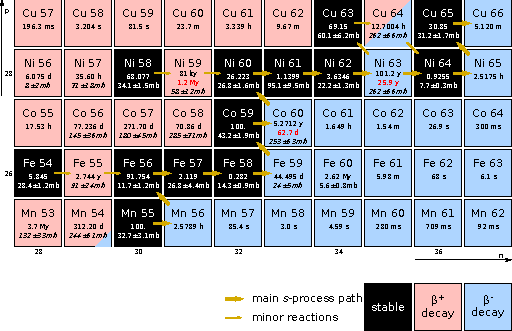
\includegraphics[width=0.9\textwidth]{graphics/s-process/feni_chartnuc}
    \caption{The \ac{sproc} around the iron peak. Due to its high abundance, \ex{56}Fe is the main seed from which the \ac{sproc} starts.}
    \label{fig:s-process:feni_chartnuc}
\end{figure}
Figure~\ref{fig:s-process:feni_chartnuc} shows an excerpt of the chart of the nuclides focusing around the iron peak. Due to its high abundance, \ex{56}Fe is the main seed for the \ac{sproc}. The thick and thin arrows in Figure~\ref{fig:s-process:feni_chartnuc} show the main \ac{sproc} path and minor reaction paths, respectively. Also given are the Maxwellian-averaged nuclear cross sections from the KADoNiS database.\footnote{\url{https://kadonis.org}} These cross sections are printed in italic if they have only been determined theoretically. Finally, half-lives are given at laboratory conditions in black and at \ac{sproc} relevant stellar conditions in red, if different.

In Figure~\ref{fig:s-process:feni_chartnuc}, for example, most of the produced \ex{63}Ni nuclei will capture another neutron in order to form \ex{64}Ni since the half-life of \ex{63}Ni is, even under stellar conditions, long enough such that this nucleus is mostly stable with respect to the \ac{sproc}. However, branching points with shorter half-lives that can have important effects on \ac{sproc} nucleosynthesis exist.


\subsection{Nuclear Reaction Rates}

We have so far mostly looked at the so-called $Q$-value, i.e., the energy released in a give nuclear reaction, in order to determine the likelihood of a reaction to take place. Energy release is however not always the dominating factor. As an example, we have discussed photodisintegration reactions, e.g., during oxygen burning -- see reactions~\eqref{eqn:massive_stars:oxygen_burning_reactions} -- that take place in massive stars even though these reactions consume energy. In a stellar environment, two additional quantities influence how likely it is for a reaction to take place. These quantities are the nuclear cross section $\sigma$ and the velocity distribution of particles in the plasma. 

Nuclear cross sections generally depend on the relative velocities of projectiles and targets, thus we can write $\sigma = \sigma(v)$. Furthermore, if the velocities follow a distribution $P(v)$ with
\begin{equation}
    \int_0^\infty P(v) dv = 1,
\end{equation}
we can write
\begin{equation}
    \int_0^\infty v P(v) \sigma(v) dv = \langle \sigma v \rangle.
\end{equation}
Here, $\langle \sigma v \rangle$ contains all information on the nuclear physics. The reaction rate $r$ for two different particles to interact can then be written as
\begin{equation}
    r = N_a N_b \langle \sigma v \rangle_{ab},
\end{equation}
where $N_a$ and $N_b$ are the respective number densities of particles $a$ and $b$. If both particles are the same this reaction rate simplifies to
\begin{equation}
    r = \frac{N_a (N_a - 1)}{2}\langle\sigma v\rangle_{aa} \overset{N_a\gg1}{\approx} \frac{N_a^2}{2}\langle\sigma v \rangle_{aa}.
\end{equation}
Using the Kronecker symbol $\delta_{ab}$, we can write the overall reaction rate for an arbitrary velocity distribution as
\begin{equation}
    r_{ab} = \frac{N_a N_b \langle\sigma v\rangle_{ab}}{1 + \delta_{ab}}.
\end{equation}
% For practical reasons, the reaction rate in the literature is often reported as $N_A \langle\sigma v\rangle_{ab}$, where $N_A = 6.022 \times 10^{23}$\,mol$^{-1}$ is the Avogadro constant.

For non-relativistic and non-degenerate stellar plasmas, the velocities of particles will follow a Maxwell-Boltzmann distribution. Depending on the temperature, the Maxwell-Boltzmann velocity distribution has its maximum at
\begin{equation}
    v_T = \sqrt{\frac{2k_B T}{m_{ab}}}. \label{eqn:s-process:max_velocity_mb}
\end{equation}
Here, $k_B = 1.380 \times 10^{-23}$\,J\,K$^{-1}$ is the Boltzmann constant and
\begin{equation}
    m_{ab} = \frac{m_am_b}{(m_a + m_b)} \label{eqn:s-process:reduced_mass}
\end{equation} 
the reduced mass of the system. The reaction rate per particle pair can then be expressed as
\begin{equation}
     \langle \sigma v \rangle_{ab} = \left( \frac{8}{\pi m_{ab}} \right)^{\nicefrac{1}{2}} (kT)^{-\nicefrac{3}{2}} \int_0^\infty E\sigma(E) \exp\left(-\frac{E}{kT}\right)dE.
 \end{equation} 

 For neutron-induced reactions, which are the ones of importance in the \ac{sproc}, the reaction rate is generally expressed in terms of a \ac{macs} as
 \begin{equation}
     \langle\sigma\rangle_T = \frac{4}{\sqrt{\pi} v_T^2} \int_0^\infty v\sigma_n(v) \left(\frac{v}{v_T}\right)^2 \exp\left[-\left(\frac{v}{v_T}\right)^2\right]dv. \label{eqn:s-process:macs}
 \end{equation}

Databases such as KADoNiS\footnote{\url{https://kadonis.org}} are generally used to look up the best \ac{macs} for a given nucleus. The total \ac{macs} are typically given at a specific energy, in KADoNiS usually at 30\,keV, which is the energy relevant for the \ac{sproc}.


\subsection{Half-Lives}

Half-lives of nuclei that disintegrate via $\beta$-decay are not always the same under laboratory and stellar conditions. One example of this is bound-state $\beta$-decay. At high temperatures, e.g., temperatures that exist in stars, a certain nucleus might have so few electrons due to ionization that it becomes unstable. In this case it would decay via $\beta^-$-decay and thus transfer a neutron into a proton and an electron. Depending on the ionization level, the half-life drastically shortens compared to neutral atoms. One example of this is \ex{187}Re. Under laboratory conditions, \ex{187}Re has a half-life or around $4.3\times10^{10}$\,a. When fully stripped however, the half-life reduces to $<100$\,a \citep{nolden97}.

Under stellar conditions and thus for highly ionized atoms, calculations for the $\beta$-decay half-lives were done by \citet{takahashi87}. These authors present decay rates for various relevant temperatures and electron number densities.


\subsection{Capturing Neutrons Slowly}

Let us first look at the horizontal transitions of the \ac{sproc}, i.e., at transitions between stable nuclei. This formalism also applies to an unstable nucleus if the half-life is long compared to the probability of capturing another neutron. The rate of change of the number density of a stable nucleus with mass number $A$ can then be written as
\begin{equation}
    \frac{dN_A}{dt} = -N_n(t) N_A \langle\sigma v\rangle_A + N_n(t) N_{A-1} \langle\sigma v\rangle_{A-1}.
\end{equation}
Here, $N_n(t)$ is the number density of free neutrons, which may very with time. Since the reaction rate depends on the velocity, which itself is defined by the temperature of the environment, we can assume that $\langle\sigma v\rangle$ is constant if the temperature does not change. 

Replacing the reaction rate per particle with the \ac{macs}, see equation~\eqref{eqn:s-process:macs}, we can write $\langle \sigma v\rangle_{A} = \langle \sigma \rangle_{A} v_T$, and thus
\begin{equation}
    \frac{dN_A}{dt} = v_T N_n(t) \left[-N_A \langle\sigma\rangle_A + N_{A-1} \langle \sigma \rangle_{A-1} \right]. \label{eqn:s-process:dna_dt_intermediate_step}
\end{equation}

Since all isotopes experience the same neutron abundance, we can introduce the neutron exposure as
\begin{equation}
    \tau = v_T \int N_n(t)dt. \label{eqn:s-process:neutron_exposure}
\end{equation}
This can also be written as $d\tau = v_T N_n(t)dt$. We can now replace the time variable $t$ in equation~\eqref{eqn:s-process:dna_dt_intermediate_step} with the neutron exposure $\tau$ and thus get
\begin{equation}
    \frac{dN_A(\tau)}{d\tau} = -N_A(\tau)\langle\sigma\rangle_A + N_{A-1}(\tau)\langle\sigma\rangle_{A-1}. \label{eqn:s-process:dna_dtau}
\end{equation}


\subsection{Local Approximations}\label{sec:s-process:local_approximation}

For the \ac{sproc} we can determine the following boundary conditions for equation~\eqref{eqn:s-process:dna_dtau}:
\begin{align}
    N_{56}(0) &= N_\mathrm{seed}\\
    N_{A>56}(0) &= 0
\end{align}
These conditions simply state that at $\tau=0$, i.e., no neutron exposure, the number density of \ex{56}Fe nuclei are equal to the total amount of seed nuclei for the \ac{sproc} and that no nuclei have been produced by the \ac{sproc} yet. 

For large \ac{macs}, the difference of $N_{A-1}(\tau) \langle\sigma\rangle_{A-1} - N_A(\tau)\langle\sigma\rangle_{A}$ becomes significantly smaller than the magnitude of either product $N_{A-1}(\tau)\langle\sigma\rangle_{A-1}$ or $N_A(\tau)\langle\sigma\rangle_{A}$. At neutron magic numbers on the other hand, where binding energies per nucleon are exceptionally high due to closed nuclear shells, the \ac{macs} become however very small. In between magic neutron numbers, e.g., for ruthenium, a steady flow along the \ac{sproc} path is achieved, which results in $dN_A/d\tau \approx 0$ and thus
\begin{equation}
    N_A(\tau)\langle\sigma\rangle_A \approx \mathrm{const.} \label{eqn:s-process:local_approximation}
\end{equation}
This effect is also known as the local equilibrium approximation and is only satisfied away from neutron-magic numbers.
\begin{figure}[tb]
    \centering
    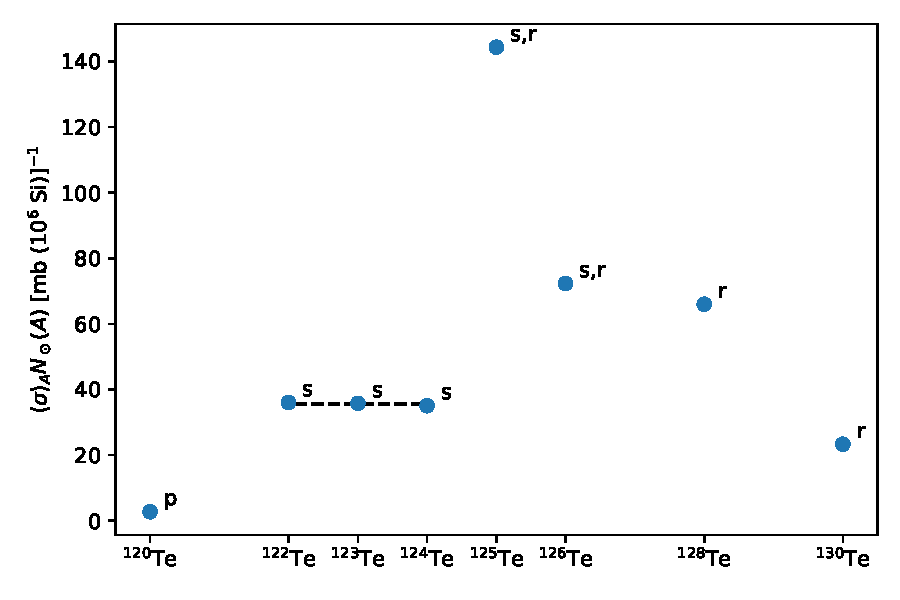
\includegraphics[width=0.75\textwidth]{graphics/s-process/local_approx}
    \caption{Product of the \ac{macs} times the solar abundance, normed to silicon equals to $10^{6}$ for various tellurium isotopes. The local approximation is nicely reproduced for the \textit{s}-only isotopes.}
    \label{fig:s-process:local_approximation_te}
\end{figure}
Figure~\ref{fig:s-process:local_approximation_te} shows the local equilibrium approximation for tellurium isotopes. Clearly, equation~\eqref{eqn:s-process:local_approximation} holds true for \ex{122}Te, \ex{123}Te, and \ex{124}Te. These isotopes are shielded by stable isobars from any contribution due to the \ac{rproc} and thus are so-called \textit{s}-only isotopes.


\subsection{Branching Points}

\begin{figure}[tb]
    \centering
    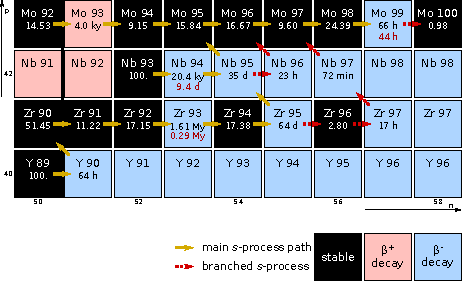
\includegraphics[width=0.82\textwidth]{graphics/s-process/zrmo_chartnuc}
    \caption{The \ac{sproc} around zirconium and molybdenum.}
    \label{fig:s-process:zrmo_chartnuc}
\end{figure}
Figure~\ref{fig:s-process:zrmo_chartnuc} shows an excerpt of the chart of the nuclides with the \ac{sproc} path indicated. Several s-called branching points exist in this mass region. Branching points, e.g., at \ex{95}Zr are points at which the \ac{sproc} can go either way and thus branches. 
The branching ratio at a given nucleus can be calculated as
\begin{equation}
    f_n = \frac{\lambda_n}{\lambda_n + \lambda_{\beta^{-}}},
\end{equation}
where $\lambda_n$ and $\lambda_{\beta^{-}}$ are the probabilities to capture another neutron and undergo a $\beta^{-}$-decay, respectively. These probabilities can be calculated as
\begin{align}
    \lambda_n &= N_n v_T \langle \sigma \rangle \\
    \lambda_{\beta^{-}} &= \frac{\ln(2)}{t_{\nicefrac{1}{2}}(T)}.
\end{align}
Here, $N_n$ is the neutron density, $v_T$ the thermal velocity as given in equation~\eqref{eqn:s-process:max_velocity_mb}, and $\langle\sigma\rangle$ the \ac{macs}. Furthermore, $t_{\nicefrac{1}{2}}(T)$ is the half-life of the nuclide of interest as a function of the temperature $T$.
\begin{figure}[tb]
    \centering
    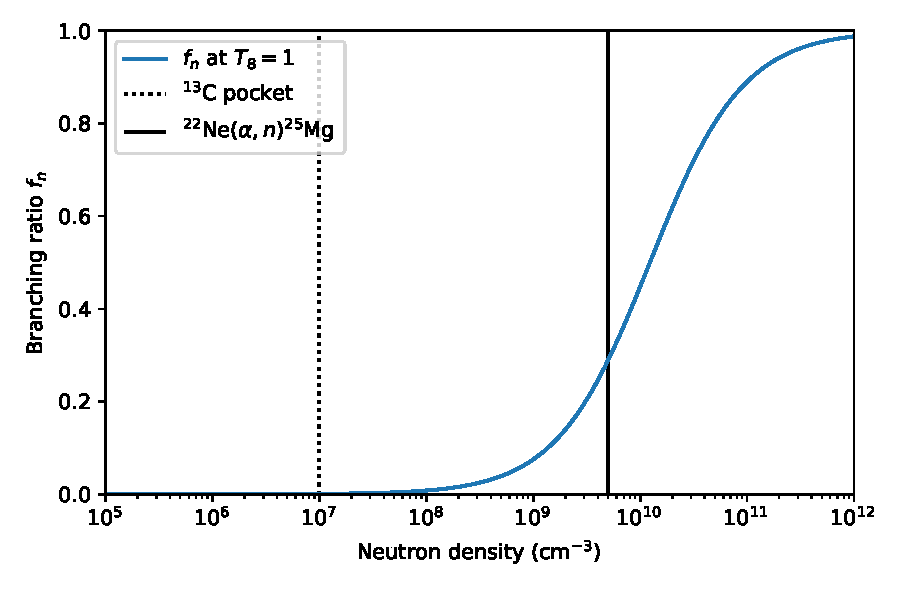
\includegraphics[width=0.75\textwidth]{graphics/s-process/branching_zr95}
    \caption{Branching ratio for \ex{95}Zr. Typical stellar regions as found in an \ac{tpagb} star are as indicated.}
    \label{fig:s-process:branching_zr95}
\end{figure}
Figure~\ref{fig:s-process:branching_zr95} shows the branching ratio for \ex{95}Zr at a temperature of $T_8 = 1$. Two regions in a \ac{tpagb} star that are discussed further below are as indicated. Clearly, neutron densities of $N_n > 10^8$\,cm$^{-3}$ are required in order to activate the branch ratio at \ex{95}Zr.


\section{Observations}

Various observations have shown that the \ac{sproc} indeed takes place in low-mass AGB stars. In 1952, \citeauthor{merrill52} observed technetium absorption lines in S-Type stars. These stars have about similar amounts of oxygen and carbon in their atmospheres and are in fact \ac{agb} stars. Technetium has no stable isotope, the longest lived one has a half-life of 4.2\,Ma and thus, this element must be produced in situ.

Further observations that significantly constrain the \ac{sproc} come from stardust grains which will be discussed in more detail in the next chapter. However, also the Solar System initial abundance shows significant \ac{sproc} contribution.

Figure~\ref{fig:solar_system_abundances} shows these abundances. Isotopes with mass numbers $A>60$ mostly formed by neutron capture, either in the \ac{sproc} or the \ac{rproc}. Certain nuclides, such as \ex{96}Mo for example, are shielded from the \ac{rproc} and lie centered on the \ac{sproc} path, see also Figure~\ref{fig:s-process:zrmo_chartnuc}. Therefore, these are \textit{s}-only nuclides that must be produced in the correct proportions during \ac{sproc} nucleosynthesis.


\section{Astrophysical Locations}

When determining the origin of certain elements and isotopes, one must always keep in mind the difference between the process that leads to the formation of a given isotope and its astrophysical location, i.e., where it takes place. In case of the \ac{sproc} the process itself has already been described in Section~\ref{sec:s-process:neutron_captures}. While the \ac{sproc} generally works as outlined above, multiple locations have been invoked that can make part of the \ac{sproc} nuclei.

\subsection{Thermally Pulsing Asymptotic Giant Branch Stars}

Low-mass \ac{tpagb} stars are thought to be the main astrophysical site for the strong \ac{sproc} and are expected to produce elements and isotopes with masses between strontium and lead. Stars that ultimately end up as \acp{wd} are considered low-mass stars, i.e., stars with masses $\leq 8\,M_\odot$. We have already discussed the evolution of the Sun, a $1\,M_\odot$ star and a schematic of its \ac{hrd} is shown in Figure~\ref{fig:sun:sun_hrd}. 
Stars with masses between approximately $2\,M_\odot$ and $4\,M_\odot$ follow a similar evolutionary path, however their helium cores do not become degenerate. No He-flash is thus experience and helium burning ignites regularly. 
Stars with initial masses $>4\,M_\odot$ undergo a second dredge-up event as they ascend the \ac{eagb} phase. The hydrogen burning in a shell restarts after this event and the star continues its development up the \ac{agb}. During the \ac{tpagb} phase, such heavy stars reach temperatures of up to 50\,MK at the bottom of the hydrogen burning shell, which can lead to nucleosynthesis via so-called hot bottom burning. Since the envelope is fully convective, the produced nuclei are rapidly recycled. 

The \ac{sproc} takes place during the \ac{tpagb} phase of these stars while hydrogen and helium burning happens alternatively. 
\begin{figure}[tb]
    \centering
    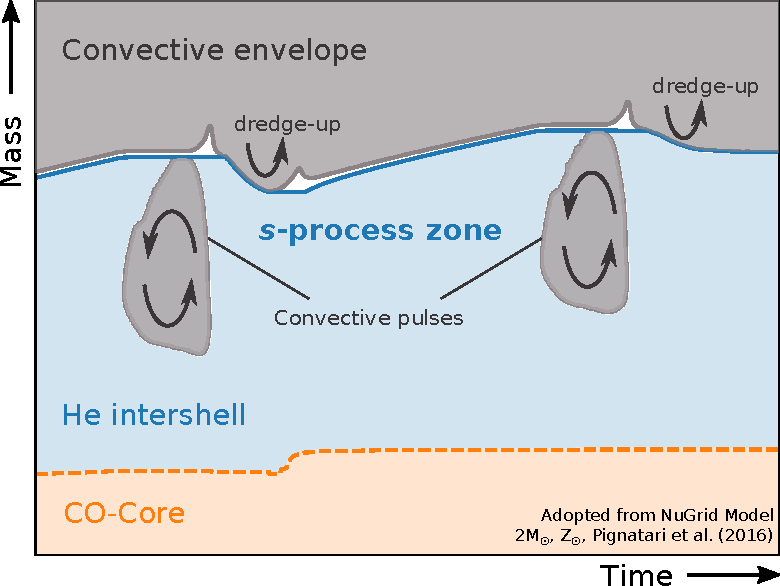
\includegraphics[width=0.7\textwidth]{graphics/s-process/kippenhahn_s-process}
    \caption{A Kippenhahn diagram of the helium intershell in which the \ac{sproc} takes place.}
    \label{fig:s-process:kippenhahn_s-process}
\end{figure}
Figure~\ref{fig:s-process:kippenhahn_s-process} shows a so-called Kippenhahn diagram of a $2\,M_\odot$ star with solar metallicity. The stellar evolution data is taken from \citet{pignatari16}. The horizontal axis depicts the time, generally in logarithmic units,\footnote{Sometimes, Kippenhahn diagrams show the model or timestep on the horizontal axis. Stellar evolution codes, when convection, activation of burning, etc., events happen, shorten the timesteps in the model in order to track these events properly. Model number or timesteps can thus be a useful alternative to physical units on the horizontal axis.} while the vertical axis shows the Lagrangian mass coordinate from the center of the star to the surface. At the bottom, shaded in orange, is the CO core of the star. The He intershell, here in blue, separates the core from the convective envelope. Furthermore, a hydrogen burning shell separates the helium intershell from the convective envelope. Once enough ashes from this burning are accumulated and have compressed the intershell, helium burning can turn on at the bottom of the shell. This leads to the formation of \ex{12}C and induces a thermal pulse, which is also known as a \acf{tdu} event. The \ac{tdu} enables mixing of material between the convective envelope and the helium intershell. 
Protons from the hydrogen envelope get mixed into the intershell, which already contains some \ex{12}C from helium burning. The \ex{12}C can now capture another neutron and form an area, here labeled \ac{sproc} zone, where \ex{13}C is abundant. The \ex{13}C can catch another $\alpha$ nucleus and undergo the reaction
\begin{equation}
    ^{13}\mathrm{C}(\alpha, n){^{16}}\mathrm{O}. \label{eqn:s-process:c13-neutron-source}
\end{equation}
This reaction releases neutrons which now become available for subsequent reactions, e.g., the \ac{sproc}. The \ex{13}C-pocket is the main neutron source for the \ac{sproc} in \ac{agb} stars. Until the next thermal pulse, it produces neutrons with a density of generally $<10^{7}$\,cm$^{-3}$ for thousands of years. Hydrogen burning continues at the bottom of the convective envelope, again compressing the intershell.

There is a fine balance of the amount of protons that can be mixed into the intershell to produce the \ex{13}C-pocket. If too few neutrons are mixed in, only little \ex{13}C is made thus limiting the effectiveness of reaction~\eqref{eqn:s-process:c13-neutron-source} as a neutron source. If too many protons are mixed in, \ex{13}C can capture another proton which leads to the formation of \ex{14}N. In addition to having destroyed a \ex{13}C nucleus, \ex{14}N also has a high neutron-capture cross section. It will thus likely undergo the reaction
\begin{equation}
    ^{14}\mathrm{N}(n,p){^{14}}C
\end{equation}
and thus actively poison the neutron source. The \ex{13}C is thus self-limiting in size.

The activation of helium burning also activates a secondary neutron source, which produces neutrons via the reaction
\begin{equation}
    ^{22}\mathrm{Ne}(\alpha, n){^{25}}\mathrm{Mg}. \label{eqn:s-process:ne22-neutron-source}
\end{equation}
Depending on the temperature at the bottom of the intershell, this neutron source only gets marginally activated. Here, for a few years, neutron densities of up to around $5\times10^{9}$\,cm$^{-3}$ can be reached. These neutron densities are high enough to activate some branching points, e.g., to branch \ex{95}Zr and form \ex{96}Zr -- see Figures~\ref{fig:s-process:zrmo_chartnuc} and~\ref{fig:s-process:branching_zr95}. For heavier stars, the \ex{22}Ne$(\alpha, n)$ neutron source get activated more since the bottom of the intershell can reach higher temperatures compared to lower mass stars.

During the intermediate \ac{tdu} events, freshly nucleosynthesized material from the helium intershell gets mixed into the convective envelope, thus enriching it in \ac{sproc} elements and isotopes. At the same time, the star is loosing mass due to the radiation pressure. While population I stars generally start their life off with carbon-to-oxygen ratios of less than one, continuous carbon production in the intershell and subsequent \ac{tdu} events mix it into the envelope. This slowly enriches the stellar composition in carbon. When the elemental C/O abundance exceeds unity, the star becomes a carbon star. The opacity in the envelope at the same time is steadily rising, which results in more mass loss. Ultimately the opacity becomes so high that most of the envelope is lost into space, which leads to the formation of a \ac{pn} and to the recycling of freshly nucleosynthesized \ac{sproc} material back into the galaxy.


\subsection{Massive Stars}

The so-called strong or main \ac{sproc} in \ac{agb} stars can only account for the solar \ac{sproc} component for elements with masses between strontium and lead. Calculations of \ac{agb} star \ac{sproc} nucleosynthesis however fall short of explaining the Solar System \ac{sproc} inventory with masses of $60 < A < 90$. 

These nuclei are made in the weak \ac{sproc} which is believed to take place during the core helium burning phase in massive stars. Nitrogen-14 nuclei that were made during the CNO cycle prior to helium burning can during this stage be transformed further to \ex{22}Ne via the reaction chain
\begin{equation}
    ^{14}\mathrm{N}(\alpha, \gamma){^{18}}\mathrm{F}(\beta^+, \gamma){^{18}}\mathrm{O}(\alpha, \gamma){^{22}}\mathrm{Ne}.
\end{equation}
At the end of the helium burning stage, the temperature in the core of these massive stars will have risen enough in order to capture further $\alpha$ particles on \ex{22}Ne and therefore enable the \ex{22}Ne$(\alpha, n)$ neutron source, see reaction~\eqref{eqn:s-process:ne22-neutron-source}. In massive stars, the dominant neutron source is thus different from the one in \ac{agb} stars, and it is thought that this weak \ac{sproc} forms the missing elements and isotopes between the iron peak and strontium.


\section{Nucleosynthesis Calculations}

Stellar nucleosynthesis calculations that describe the \ac{sproc} are generally using 1D stellar evolution models. Higher dimensional effects, such as rotation, can still be implemented by applying intermediate mixing steps. Since \ac{sproc} nucleosynthesis involves many isotopes and reaction rates, running a full nucleosynthesis calculation inside the stellar evolution model is computationally expensive. Therefore, stellar evolution is generally modeled using a very limited set of isotopes and reactions, in fact only the ones that produce energy and thus contribute to heat and radiation inside the star. Neutron capture reactions on the other hand are not energy producing and thus can be calculated in a post-processing step, i.e., separately from nucleosynthesis calculations.

In addition to the NuGrid collaboration, which publishes all stellar evolution models and post-processing output along with their scientific research (see page~\pageref{codebox:nugrid}), Italian researchers around Sergio Cristallo, Oscar Straniero, and many more also make their modeling results for \ac{sproc} nucleosynthesis available online. The output of the \ac{fruity} models are available online in a searchable and well-documented database.\footnote{\url{http://fruity.oa-teramo.inaf.it/modelli.pl}} Many models are available and can be browsed. These \ac{fruity} models are furthermore interesting since they are the only ones that incorporate the full nucleosynthesis network into the stellar evolution model. 


\section{Reading}

Please read \citet{gallino98}, a key paper on \ac{sproc} nucleosynthesis. This paper contains a total of 20 figures, many of them show similar simulations with different inputs. Please have a look at all figures and try to understand what the authors are demonstrating in them. Feel free to skim through certain sections that are not as relevant to the discussion. The following list defines some topics that we will talk about in class.
\begin{itemize}
    \item How and where does the \ex{13}C-pocket form in the \ac{sproc} model by \citet{gallino98}?
    \item What does it mean when \citet{gallino98} write that the \ex{13}C pocket is of primary origin?
    \item What is the main component of the \ac{sproc} and how is it determined?
    \item What are the main neutron sources and why? Which one is more important and how does this importance change among different models, i.e., how do temperature and stellar mass influence the neutron sources?
    \item What observations are the model calculations compared to?
    \item Why is the \ex{13}C pocket self-limiting? Why can't it be smaller / larger than a certain value?
    \item How does the initial metallicity of a star affect its \ac{sproc} output?
\end{itemize}

%!TEX root = origin_elements_lecture_notes.tex

\chapter{Stardust}\label{ch:stardust}

Researchers around Ed Anders and Roy Lewis at the University of Chicago were puzzling over isotope anomalies found in meteorites. Some primitive meteorites showed strange isotopic compositions in certain noble gas isotopes that did not fit into the Solar System. Furthermore, these isotopic abundances were weird since they could not easily be explained by any chemical process. The researchers separated the meteorite into individual parts in the hope of isolating the carrier of these anomalies, which they ultimately, discovered: interstellar nanodiamonds \citep{lewis87}. For the curious reader, a detailed review on astrophysics with extraterrestrial material was recently presented by \citet{nittler16}.


\section{The Origin of Stardust}

\begin{figure}[tb]
    \centering
    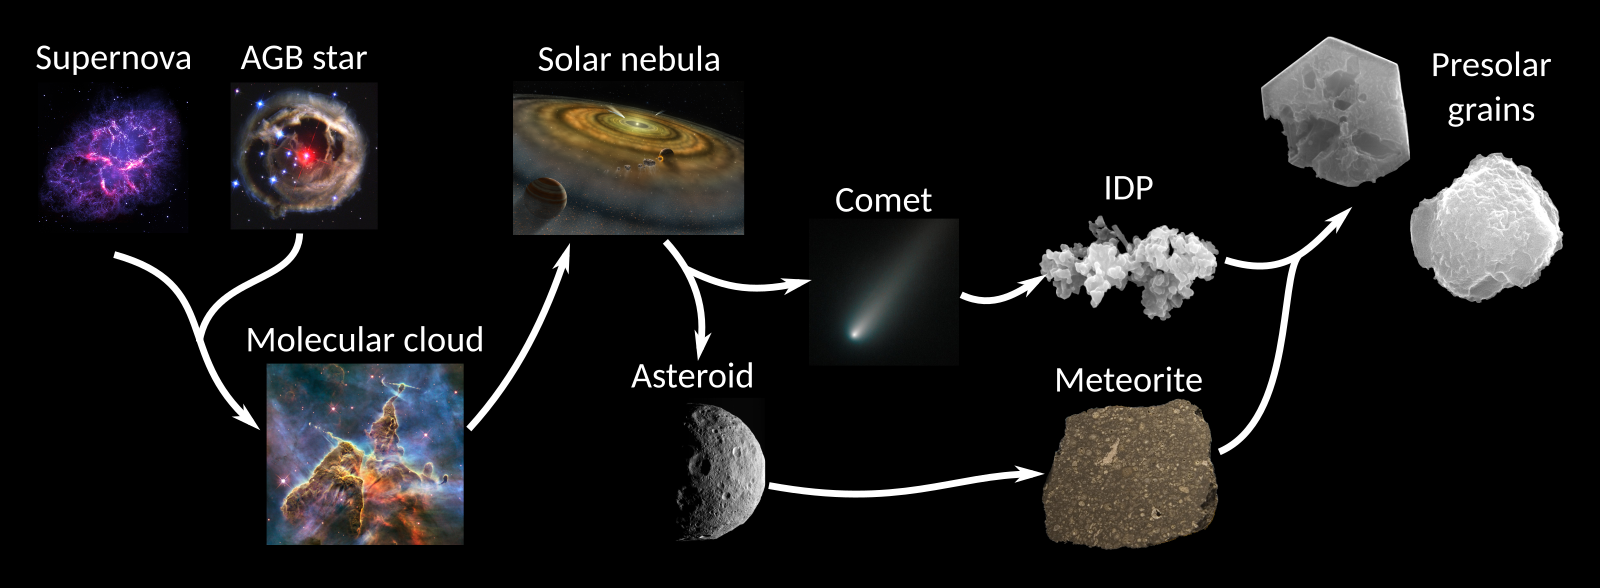
\includegraphics[width=0.9\textwidth]{graphics/stardust/presolar_grains_origin_1600}
    \caption{Schematic of the origin of stardust grains.}
    \label{fig:stardust:origin_of_stardust_schematic}
\end{figure}
The origin of stardust grains is summarized schematically in Figure~\ref{fig:stardust:origin_of_stardust_schematic}
These grains formed in the death throes of dying stars and got subsequently recycled into the interstellar medium. Some of these particles became part of the molecular cloud from which the Solar System formed. Since they represent samples from before the solar nebula, they are also often referred to as presolar grains. During the formation of the first solids in the Solar System, stardust grains were incorporated into meteorite parent bodies. Some primitive meteorites, see discussion in Chapter~\ref{ch:solar_system_abundances}, have preserved these particles up to today. Stardust grains can thus be found in primitive meteorites and can be separated from them for subsequent studies. The grains are especially variable since they carry the nucleosynthetic fingerprint of their parent star.

Stardust grains are generally discovered due to their extreme isotope anomalies, which are very distinct from the solar composition. While their composition cannot be explained by any processes found in the Solar System, they agree astonishingly well with nucleosynthesis predictions of stars, e.g., \ac{sproc} nucleosynthesis in \ac{agb} stars.


\subsection{Types of Stardust Grains}

The most abundant type of stardust grains are nanodiamonds. True to their name, these particles are only a few nanometers in diameter and thus currently still too small in order to study directly in the laboratory. However, recent advances in mass spectrometry have allowed to directly study at least their carbon isotopic composition on a per-grain basis \citep{heck14}. As proposed before \citep{lewis87}, nanodiamonds carry, e.g., the xenon isotopic anomalies. Measuring the size distribution of nanodiamonds and the amount of anomalous xenon, only one in $10^6$ nanodiamonds is actually expected to carry a single xenon atoms. This further complicates research on these phases.

One of the best studied phases of stardust grains are presolar \ac{sic} grains. These particles can be separated from meteorites and thus studied individually in the laboratory. Since \ac{sic} grains frequently occur in sizes of up to several micrometers, they have also been intensively analyzed in the past. Details on these grains are discussion in Section~\ref{sec:stardust:sic_grains}.

Graphite grains can also be gently separated from meteorites. These grains also show up in large sizes, however, graphite can act like a sponge for other elements and thus, the original stellar signal often shows contamination with solar system material.

Finally, in situ detection techniques have allows the search for other types of stardust grains in sections of meteorites. Depending on the type of meteorite, various concentrations of other stardust grains have been found, e.g., silicates, oxides, etc. These grains are usually sub-micrometer in size and thus difficult to analyze. Since they cannot be easily separated from their host meteorite, analyses are more complicated and time-consuming.




\subsection{Separation of Stardust Grains}

Presolar grains such as nanodiamonds and \ac{sic} grains are separated from meteorites using a suite of crushing, freeze-thaw cycles, and chemical treatments. This methodology has also been appropriately referred to as finding the needle in the haystack by burning down the hay. 

Usually, a few grams of a meteorite are taken and first crushed with a mortar and pestle. This breaks the big grains apart. Subsequently, the powder is submerged in water and several freeze-thaw cycles are used in order to break the dust further down into individual component. Once this additional crushing is finished, the burning of the hay begins. Using various acids, material that makes up all the solar system ``stuff'', e.g., the silicates, organic material, etc., are dissolved. After each acid step, remaining solids are separated from the liquid by centrifugation and the liquid is decanted or pipetted off. Finally, only presolar \ac{sic} grains and the hardiest phases that form in the solar system should be left over, among which are \href{https://en.wikipedia.org/wiki/Spinel}{spinels}. These phases have different densities from the stardust grains and can thus be separated further using heavy liquids. For example, spinel has an average density of 3.64\,g\,cm$^{-3}$,\footnote{\url{http://webmineral.com/data/Spinel.shtml}} while \ac{sic} has an average density of 3.21\,g\,cm$^{-3}$.\footnote{\url{http://webmineral.com/data/Moissanite.shtml}}

During all of these steps, extreme care has to be taken in order to (1) not loose the micrometer-sized \ac{sic} grains and (2) to not contaminate them with solar material. Therefore, only the cleanest possible acids and other chemical are used in these separation procedures. These separation procedures take weeks to months and grains need to be subsequently mounted for further analysis. This is usually done by mounting SiC grains onto ultra-pure gold foil.
\begin{figure}[tb]
    \centering
    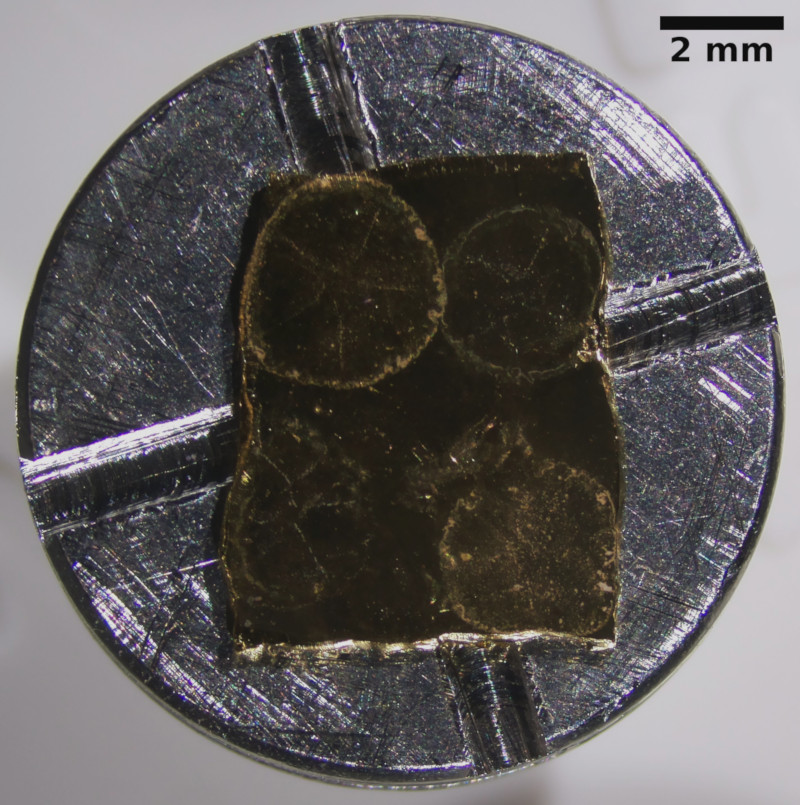
\includegraphics[width=0.35\textwidth]{graphics/stardust/standard_mount}
    \caption{A standard for presolar grain analysis mounted in the same way as actual samples would be mounted. Due to the high density of the standard, it can actually be seen in this image as rings.}
    \label{fig:stardust:sample_mount}
\end{figure}
Figure~\ref{fig:stardust:sample_mount} shows an image of a sample mount onto which four different standards were loaded. As for presolar grains, standards are drop deposited onto ultra-clean gold. Here, four distinct rings can be seen. Compared to samples, standards are mounted in a higher density, which makes the material visible.


\subsection{In Situ Analyses}

In comparison to stardust grain separations, in situ searches of meteorite slices can also be performed. Here, researchers usually use ion imaging techniques (see next section) in order to search for isotopically anomalous spots in a given meteorite. For example, a meteorite slice can be imaged to search for anomalies in the oxygen isotopic composition. While all phases from the Solar System generally plot in a very constrained area in terms of isotopic ratios, presolar grains can vary massively from the solar composition. Thus, these grains will stick out in ion images as hot spots.



\section{Measurement Techniques}

Many micro- and nanoscale techniques are required in order to study stardust grains. Here we will focus strictly on state-of-the art analysis of the isotopic composition of presolar grains. Further techniques, e.g., to study the crystal structure, of these grains, can be found in the literature \citep[see, e.g.,][and references therein]{nittler16}.

\subsection{Secondary Electron Microscopy}

In order to locate and identify the stardust grains of interest on a gold mount, \acf{sem} is used to image the mount first. Here, an electron beam is scanned over the surface and the intensity of secondary electrons are measured to reconstruct an image. Any kind of microscopy is limited to how small a feature it can detect by its wavelength. This is also known as the Abbe diffraction limit, which states that
\begin{equation}
    d = \frac{\lambda}{2n\sin(\theta)}.
\end{equation}
Here, $d$ is the minimum resolvable distance, $\lambda$ the wavelength, $n$ the refractive index of the medium, and $\theta$ the half-angle of the spot the beam of light is converting to. Usually, $n\sin(\theta)$ is also called the numerical aperture of a system and, in modern microscopes, can achieve values 1.4-1.6. The wavelength of electrons is a lot shorter than the wavelength of light, thus \acp{sem} can achieve a much higher resolution.
\begin{figure}[tb]
    \centering
    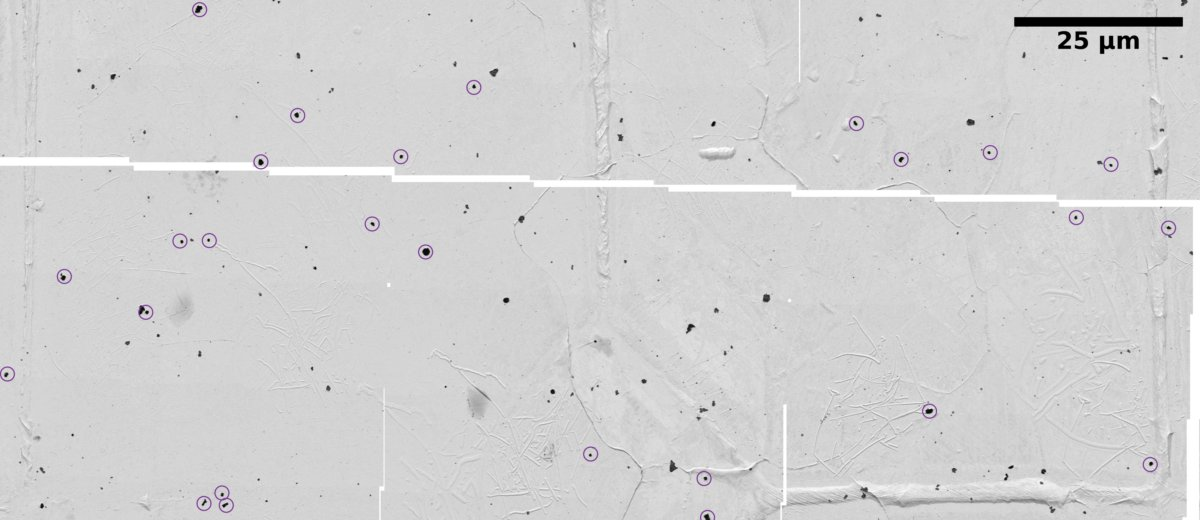
\includegraphics[width=\textwidth]{graphics/stardust/sem_mount-s}
    \caption{Small section of a presolar grain gold mount imaged in an \ac{sem}. Identified \ac{sic} grains are circled in purple.}
    \label{fig:stardust:sem_stardust_mount_map}
\end{figure}
Figure~\ref{fig:stardust:sem_stardust_mount_map} shows a fraction of a stardust gold mount imaged in the \ac{sem}. Here, backscattered electrons, which elastically scatter of the sample, were detected for generating the image. Heavy elements backscatter electrons more strongly than light ones. Therefore, gold is shown as a bright surface while \ac{sic} grains are dark. 

Imaging mounts however is not good enough since separation of stardust grain can always leave some other material behind. Therefore, \ac{sic} also have to be identified by elemental mapping to ensure that silicon and carbon are present. This is usually done by \acf{edx}. Irradiating the sample with the electron beam in an \ac{sem} excites the sample's electrons. When these electrons fall back into their ground state they emit X-rays, which are characteristic of the element itself. By analyzing these X-rays, the composition of the imaged sample can be determined. In Figure~\ref{fig:stardust:sem_stardust_mount_map}, identified \ac{sic} grains are marked with purple circles. Imaging and mapping of stardust grain mounts can generally be done automatically and can take up to sever days, depending on the resolution required. These maps usually contain thousands of images, poorly overlapping image boarders can be seen in Figure~\ref{fig:stardust:sem_stardust_mount_map}. Subsequent marking of the grain mount can also be automated, e.g., using imaging software such as ImageJ.\footnote{\url{https://imagej.nih.gov/ij/}}


\subsection{Mass Spectrometry}

While elemental analysis that rely on electron transitions can be done in a non-destructive way, no method to date exists to analyze the overall isotopic composition. However, mass spectrometry techniques with high enough spatial resolution in order to analyze individual grains have been developed. Here, two of these techniques that are regularly applied to stardust analysis are described in detail. These two techniques are the main drivers to analyze the stardust grains for their isotopic nucleosynthesis fingerprints.

The principal setup of every mass spectrometer can be broken into three main parts. First, an ion source must be present that can take the given sample and ionize its constituents. In the case of presolar grains the ion source needs to remove material from the grain and ionize it. Second, a mass analyzer then separates the ions by their respective mass-over-charge ($m/q$) ratio. Third, these separated ions must be detected in a detector system.


\paragraph{NanoSIMS} The \acf{nanosims} instrument is built by the French company CAMECA.\footnote{\url{https://www.cameca.com/}} It has been available commercially for around 20\,years and, during this time, has been updated several times. 
\begin{figure}[tb]
    \centering
    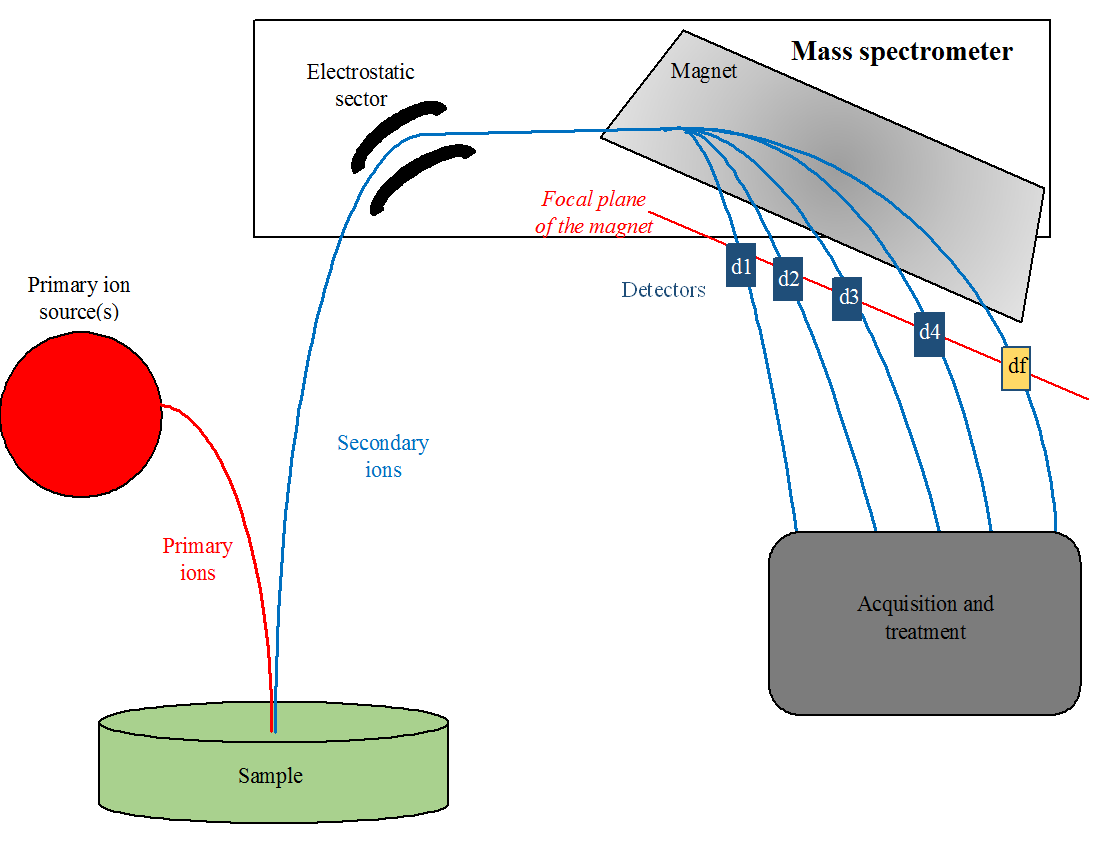
\includegraphics[width=0.6\textwidth]{graphics/stardust/nanosims}
    \caption{Schematic inner working of a \ac{nanosims}. Credit: Eden Camp via \href{https://en.wikipedia.org/wiki/Nanoscale_secondary_ion_mass_spectrometry}{Wikipedia}.}
    \label{fig:stardust_nanosims_schematic}
\end{figure}
Figure~\ref{fig:stardust_nanosims_schematic} shows a schematic of the inner workings of a \ac{nanosims}. 
In a NanoSIMS, sample material is removed from the surface using an ion gun, usually either by using Cs$^{+}$ or O$^{-}$ ions. Depending on the exact setup, the ion beams can be focused down to usually tens of nanometers. The size of this ion beam also defines the spatial resolution that can be achieved by the instrument. When the ion beam hits the surface, sample material is sputtered off. Some small fraction of this sample material is ionized directly due to the interaction with the ion beam. This directly ionized fraction, which is usually $\ll1\%$ of the total sputtered material, is then focused with various electrostatic lenses and transported to a magnetic sector. When passing through the magnetic field $\vec{B}$, the Lorentz force $\vec{F}_L$ will separate the ions by $m/q$:
\begin{equation}
    \vec{F}_L = q(\vec{E} + \vec{v} \times \vec{B})
\end{equation}
The electric field $\vec{E}$ can be neglected in a magnetic sector and the separation is solely due to the magnetic field $\vec{B}$. Individual, separated ion beams are then detected. Depending on the amount of signal, this detection either takes place via secondary electron detectors, which amplify the signal and are thus used for low count rates, or using Faraday cups that simple measure the total number of ions arriving using a current meter.

In order to calibrate the detector and the ionization probability, standards with known composition are often used. For example: when measuring presolar \ac{sic} grains for their carbon and silicon isotopic composition, terrestrial \ac{sic} can be used as a standard material. Since stardust grains show large isotopic variations compared to material that originated from within the Solar System, these standard materials can be assumed to have solar composition.

While \ac{nanosims} is a valuable technique to analyze stardust grains, the low secondary ion yield achieved by sputtering limits the technique's applicability to major elements in these samples. Furthermore, since ions are separated by $m/q$, isobaric interferences can occur depending on the elements of interest. For example, when analyzing the iron isotopic composition of a given stardust grain, the abundance of \ex{58}Fe cannot be measured since it would be overshadowed by \ex{58}Ni (see, e.g., Figure~\ref{fig:s-process:feni_chartnuc}). Similarly, \ex{64}Ni cannot be distinguished from \ex{64}Zn. Other techniques are thus required in order to remove isobaric interferences and achieve higher sensitivity. 


\paragraph{RIMS}

To achieve higher sensitivity and suppress isobaric interferences, \acf{rims} can be used to analyze stardust grains. 
\begin{figure}[tb]
    \centering
    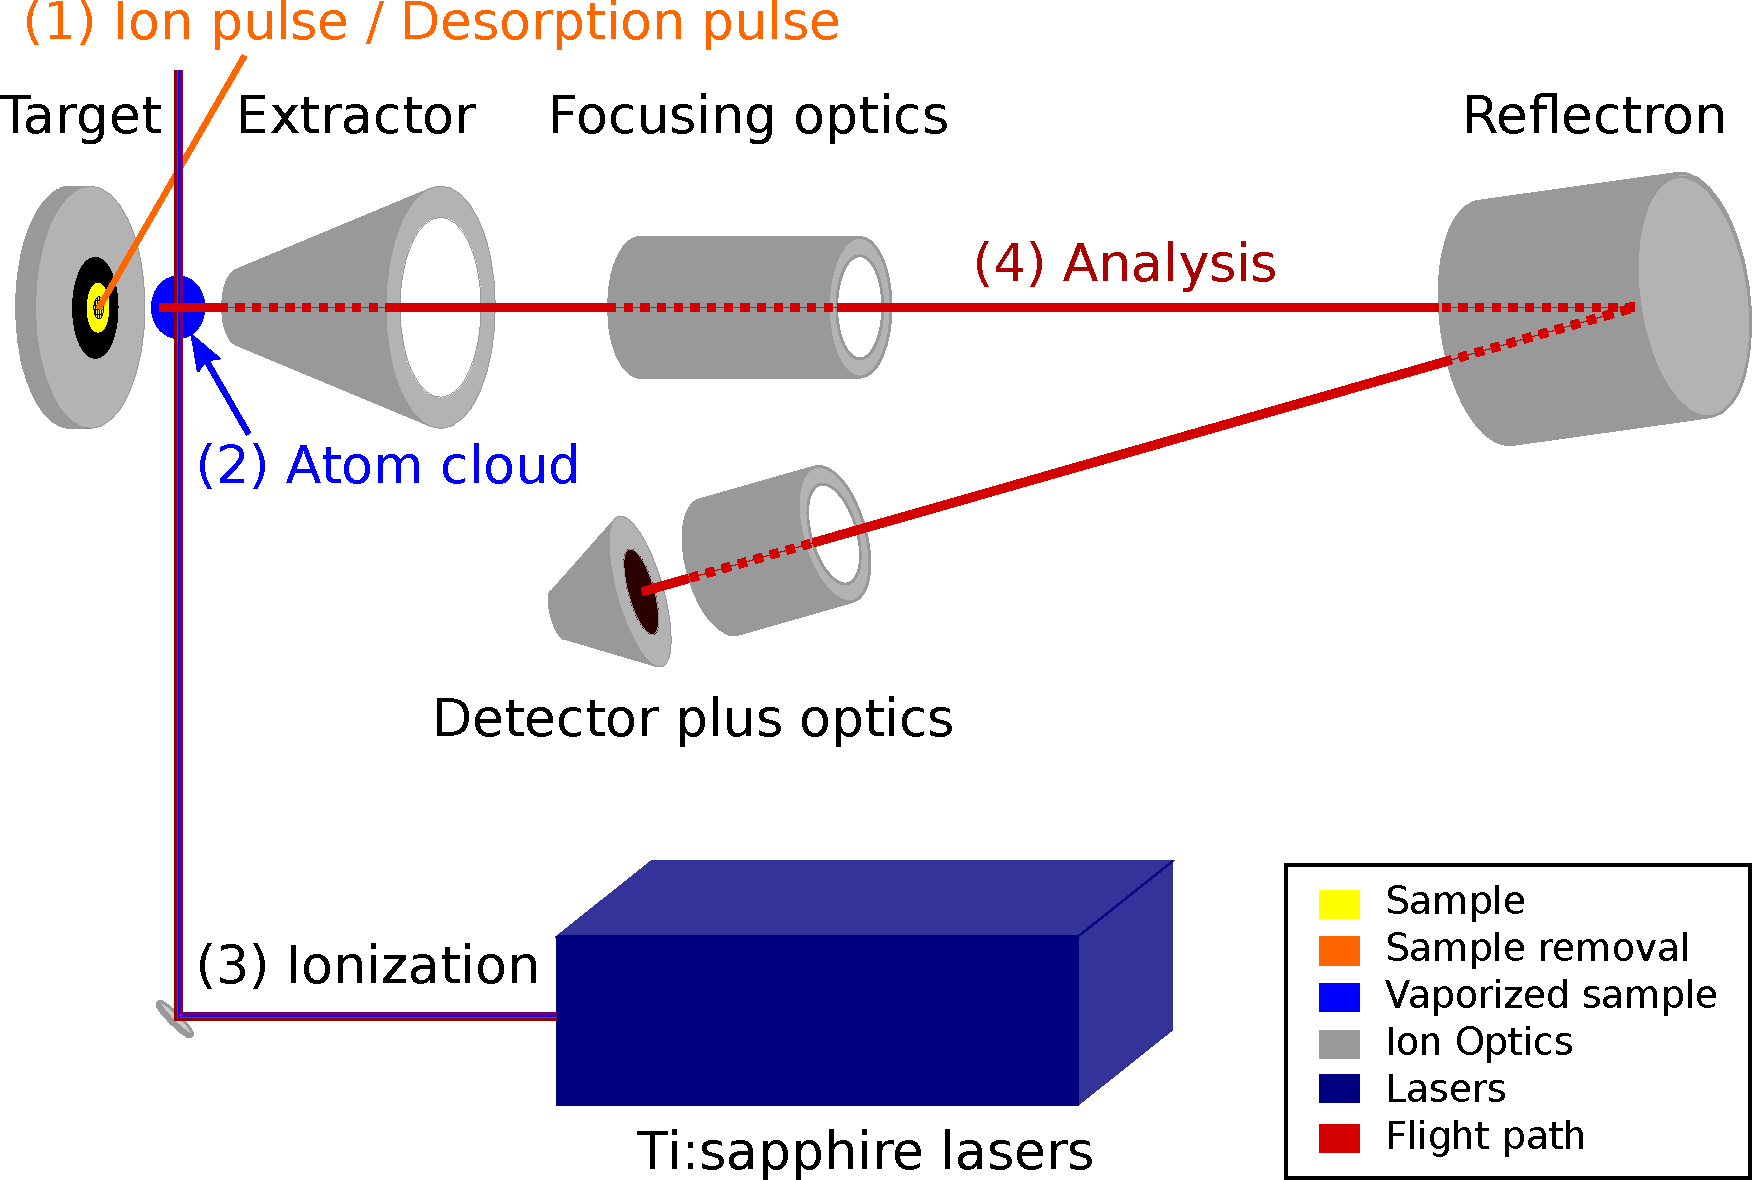
\includegraphics[width=0.7\textwidth]{graphics/stardust/rims_schematic}
    \caption{The inner workings of \ac{rims}. Details are described in the text.}
    \label{fig:stardust:rims_schematic}
\end{figure}
Figure~\ref{fig:stardust:rims_schematic} shows a schematic of the inner workings of a \ac{rims} instrument. Numbered steps in the figure are also numbered in the following text. Sample material from a target are removed (1) either using an ion gun, similar to \ac{nanosims}, or a desorption laser. For stardust grain analysis, sample material is generally removed using a desorption laser, which can achieve a spatial resolution of down to $\sim1\,\mu$m. After sample removal, a cloud of neutral atoms (2) and secondary ions exists above the sample. Secondary ions are then ejected from the system by pulsing the extractor optics to high voltages, thus removing these ions from the cloud. Neutral atoms, left behind after this ejection, are then ionized resonantly (3) using tunable \acf{tisa} lasers. The ions are then extracted into a \acf{tof} mass spectrometer, the mass analyzer. Finally, the total flight time of the ions is detected and recorded. This procedure is repeated in modern RIMS instruments at frequencies of 1\,kHz and above. Thus, over time an overall mass spectrum of the sample and its isotopic composition is acquired.

Resonance ionization is highly mass selective. 
\begin{figure}[tb]
    \centering
    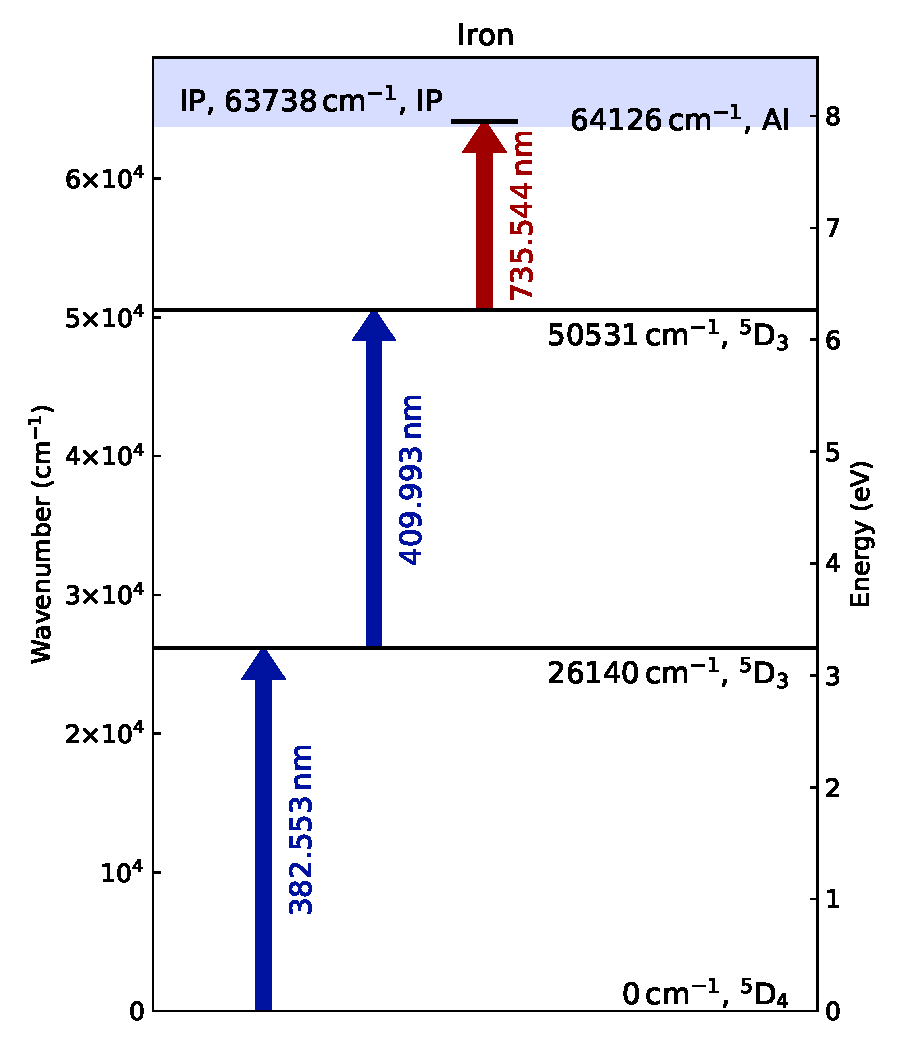
\includegraphics[width=0.49\textwidth]{graphics/stardust/fe_ionization_scheme}
    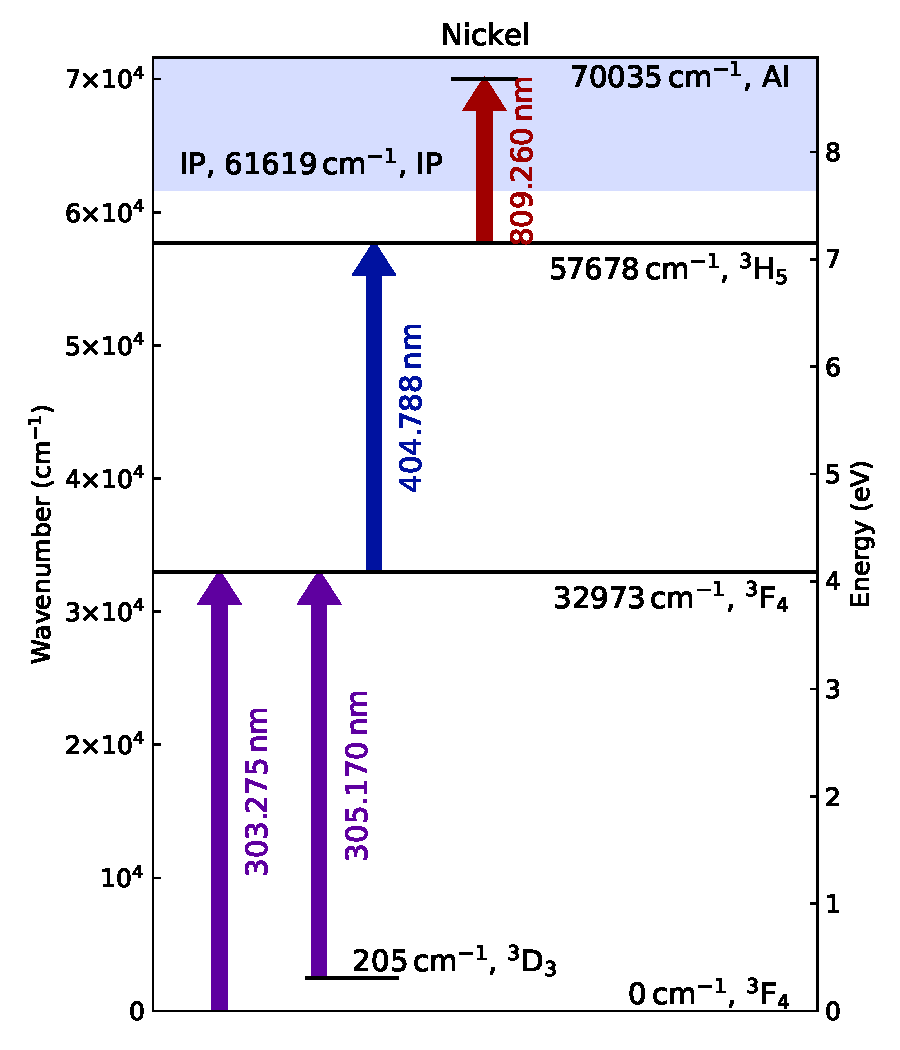
\includegraphics[width=0.49\textwidth]{graphics/stardust/ni_ionization_scheme}
    \caption{Resonance ionization schemes for iron (left) and nickel (right). Figures were created using a \ac{rims} scheme drawer available on \href{https://github.com/RIMS-Code/RIMSSchemeDrawer}{GitHub}.}
    \label{fig:stardust:fe_ni_ionization_schemes}
\end{figure}
Figure~\ref{fig:stardust:fe_ni_ionization_schemes} shows two resonance ionization schemes for iron (left) and nickel (right). Each scheme uses multiple steps in order to ionize an element of interest. These individual steps are highly element specific, which therefore mostly eliminates isobaric interferences in \ac{rims}. Furthermore, since ionization works on the neutral atoms, which are by far the majority of the sputtered or desorbed material from the sample, \ac{rims} is also much more sensitive than, e.g., \ac{nanosims}. \citet{savina18} have shown an overall useful yield for uranium measurements of 38\%. This means that 38\% of all atoms removed from a specific sample have been detected afterwards. However, the laser requirements makes \ac{rims} more complicated and to-date, no commercial mass spectrometer is available. In fact, only two \ac{rims} exist worldwide that focus on stardust analysis, namely the \ac{chili} at the University of Chicago and the \ac{lion} instrument at Lawrence Livermore National Laboratory. 

After ionization, isotopes are separated by $m/q$ in the \ac{tof} mass analyzer. Here, the extractor gives each ion the same amount of energy. Depending on the voltage field the ions go through, their energy becomes $E_\mathrm{el} = q U$, where $q$ is their charge and $U$ is the voltage field. This energy is equal to the kinetic energy $E_\mathrm{kin} = 0.5 m v^2$ of the individual ions. Since the ions have different masses, they will end up having different energies and thus different velocities. Heavier isotopes arrive at the detector later and for a given distance $d$, the total flight time is 
\begin{equation}
    t \propto \sqrt{\frac{m}{q}}.
\end{equation}
The proportionality constant depends on the instrumental setup. 

\begin{figure}[tb]
    \centering
    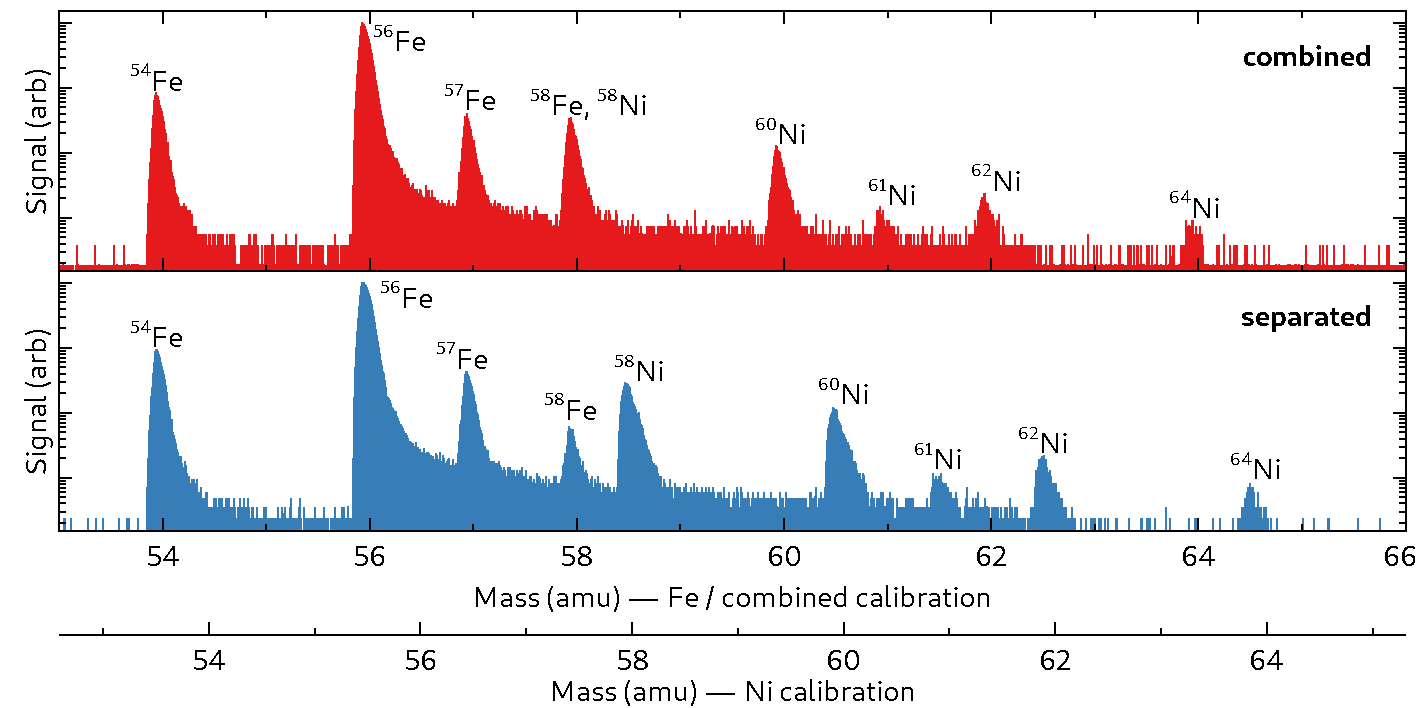
\includegraphics[width=\textwidth]{graphics/stardust/feni_ms}
    \caption{Simultaneous measurement of iron and nickel by \ac{rims}. The top panel shows the overlap of the two spectra at mass 58, in the bottom spectrum these peaks are separted by shifting the timing of the ionization lasers. Figure created with \href{https://veusz.github.io}{Veusz}.}
    \label{fig:stardust:fe_ni_rims_ms}
\end{figure}
Figure~\ref{fig:stardust:fe_ni_rims_ms} shows a \ac{rims} measurement of all iron and nickel isotopes using the ionization schemes shown in Figure~\ref{fig:stardust:fe_ni_ionization_schemes}. Simultaneous analysis of these two elements show the isobaric inferences at mass 58 (see top panel). With \ac{rims} however, the ionization is not dependent on the ion sputtering event, but rather on the laser ionization pulses. Since \ac{tof} mass spectrometry requires the whole system to be pulses, ionization timings can simply be moved with respect to each other in order to shift mass peaks apart. For the bottom panel in Figure~\ref{fig:stardust:fe_ni_ionization_schemes} this has been done for the iron and nickel measurements. The nickel ionization lasers fire around 200\,ns after the iron ionization lasers, which results in an apparent mass shift. Thus, all isotopes can be detected without isobaric interferences. 

\begin{figure}[tb]
    \centering
    \includegraphics[width=\textwidth]{graphics/stardust/lion}
    \caption{The \ac{lion} instrument at Lawrence Livermore National Laboratory.}
    \label{fig:stardust:lion_photo}
\end{figure}
While many more pages could be written on the beauty of \ac{rims} and its advantages, the curious reader shall hereby be referred to a recently published book chapter \citep{savina21}. An open-access \ac{pdfdoc} version can also be found on the U.S. Department of Energy's Office of Science and Technology Website.\footnote{\url{https://www.osti.gov/servlets/purl/1763939}} Finally, Figure~\ref{fig:stardust:lion_photo} shows an image of the \ac{lion} instrument at Lawrence Livermore National Laboratory. Six tunable \ac{tisa} lasers are shown on the left, the mass spectrometer stands on the right-hand side of the image. The reflectron is out of view on top of the photograph.




\section{Silicon Carbide Grains} \label{sec:stardust:sic_grains}

After having extensively discussed the separation and measurement techniques to analyze stardust grains, let us in brief see what measurements of these grains show. The discussion here mainly focuses on presolar grain classification. More analysis and comparisons with \ac{sproc} models will be discussed in the reading.


\subsection{Notation}

Stardust grains are generally analyzed by mass spectrometry for their isotopic composition. While elemental concentrations can be measured as well, such analyses are preferentially used to trace stardust grain condensation processes and not necessarily nucleosynthesis itself. Isotope measurements are usually expressed as ratios with respect to the most abundant isotope. While direct ratios are used for huge differences, smaller anomalies are usually expressed a permil deviations from the solar composition as so-called $\delta$-values. For any given isotope ratio $^{i}X/^{j}X$ of element $X$ can be written in $\delta$-notation as:
\begin{equation}
    \delta\left(\frac{^iX}{^jX}\right) = \delta {^{i}}X_{j} =  \left[\frac{\left(\frac{^iX}{^jX}\right)_\mathrm{sample}}{\left(\frac{^iX}{^jX}\right)_\odot} - 1\right] \times 1000 \qquad (\permil) \label{eqn:stardust:delta_notation}
\end{equation}
Here, the expression in square brackets defines the $\delta$-value. Multipling this value by 1000 is generally done in order to express this deviation in permil.


\subsection{Classification of \ac{sic} grains}

\begin{figure}[tb]
    \centering
    \includegraphics[width=0.49\textwidth]{graphics/stardust/sic_n_c_all}
    \includegraphics[width=0.49\textwidth]{graphics/stardust/sic_si_3iso_all}
    \caption{Nitrogen, carbon, and silicon isotopic composition of analyzed \ac{sic} grains. Data taken from the \href{https://presolar.physics.wustl.edu/presolar-grain-database/}{presolar grain database}.}
    \label{fig:stardust:classification_c_n_si_data}
\end{figure}
Figure~\ref{fig:stardust:classification_c_n_si_data} shows \ac{sic} the nitrogen isotopic ratio as a function of the carbon isotopic ratio (left) and a silicon three isotope plot (right) for \ac{sic} grain measurements. The axes in the left figure show isotope ratios directly and are both scaled logarithmically. This demonstrates the huge variations in the carbon and nitrogen isotopic composition that stardust grains manifest. Note that the cyan box in the middle shows the total variation, especially of nitrogen isotopes, in the Solar System. Until measurements using samples from the Genesis spacecraft were performed \citep{marty11}, the actual nitrogen isotopic composition of the Sun was poorly understood since large variations of this isotope ratio are found in the Solar System. The range shown in Figure~\ref{fig:stardust:classification_c_n_si_data} (left) is taken from \citet{fueri15}. 

The nitrogen and carbon isotopic compositions can be associated with various nucleosynthetic sources. Clearly established astrophysical sites exist for mainstream (M) and type X presolar grains.\footnote{Type X presolar grains were originally named for their eXtreme isotope ratios.} Type Y and Z grains likely originated from AGB stars as well, probably though from stars with subsolar metallicities. Type AB grains were originally defined as two different groups, however, more data showed one population and these measurements were thus grouped together. Recent studies however indicate multiple origins for type AB grains again. Finally, Type N grains were originally thought to come from novae, however, more studies have shown that surely part of their population originated in supernovae. 

The silicon isotopes, shown on the right in Figure~\ref{fig:stardust:classification_c_n_si_data} as $\delta$-valeus also show a lot of spread. Noticeable features are that X grains seem to be heavily enriched in \ex{28}Si compared to the Solar System. Mainstream grains, originating from AGB stars, all lie on a slope 1.4 line and are for the most part enriched in \ex{29}Si and \ex{30}Si compared to the Solar System.

While measurements of nitrogen, carbon, and silicon are indicative of a stardust grain's origin, other smoking gun measurement have in fact proven the sample's provenance. For grains from supernovae, measurements have shown that they condensed with live \ex{44}Ti, a \ac{slr} with a half-life of $t_{\nicefrac{1}{2}} = 60$\,a. After incorporation, \ex{44}Ti decayed to its stable daughter \ex{44}Ca, which occurs in stardust grains from supernovae in large abundances. Stardust grains from \ac{agb} stars on the other hand show typical \ac{sproc} patterns for elements like strontium, zirconium, molybdenum, etc., thus clearly showing their origin.



\subsection{Constraining \textit{s}-process nucleosynthesis}

\begin{figure}[tb]
    \centering
    \includegraphics[width=0.6\textwidth]{graphics/stardust/zr_s-proc}
    \caption{Zirconium isotope measurements by \citet{barzyk07} in comparison with \ac{agb} star models by \citet{lugaro18}.}
    \label{fig:stardust:zr_comparison_barzyk_lugaro}
\end{figure}
The clear \ac{sproc} signatures in \ac{sic} M grains not only show their provenance, but can also be analyzed in order to better understand the parent stars they formed in.
Figure~\ref{fig:stardust:zr_comparison_barzyk_lugaro} shows zirconium isotope measurements by \citet{barzyk07} in comparison with \ac{agb} star models by \citet{lugaro18}. The $\delta^{96}\mathrm{Zr}_{94}$ ratio shows the amount of branching that takes place in the star, see, e.g., Figures~\ref{fig:s-process:zrmo_chartnuc} and~\ref{fig:s-process:branching_zr95}. If all other parameters are left the same, heavier stars will activate the \ex{22}Ne$(\alpha,n)$ neutron source more efficiently since the temperature at the bottom of the helium intershell is higher. Thus, \ex{95}Zr can be branched more effectively, yielding a higher production of \ex{96}Zr. In Figure~\ref{fig:stardust:zr_comparison_barzyk_lugaro}, all thermal pulses are plotted with symbols and not just lines if the carbon-to-oxygen ratio in the convective envelope exceeds unity. This elemental ratio is required for \ac{sic} to form in the stellar envelope. If more oxygen is present in the envelope, all silicon will form bonds with oxygen assuming a perfectly mixed envelope. Since \ac{sic} can only condense when $\mathrm{C}/\mathrm{O}>1$, the grains can also only trap the nucleosynthetic fingerprint of their parent star at that moment. 

In recent years, significant process has been made on \ac{sproc} nucleosynthesis, especially thanks to efforts by Nan Liu and collaborators. The curious reader is point to check out her publications for further study.\footnote{\url{https://scholar.google.com/citations?user=dGoIdFgAAAAJ}}


\subsection{Supernova condensations}

In addition to studying the \ac{sproc}, \ac{sic} X grains can also be used to analyze output from \acp{sn}. While the measurement techniques are identical to other \ac{sic} grains, the interpretation of the data is more difficult. Studies of \ac{agb} stars have the advantage that everything formed from a homogeneous composition in the convective envelope. \acp{sn} on the other hand are generally only modeled in 1D but clearly show asymmetric explosion patterns in 3D. Inhomogeneous mixing is difficult to constraint.

Recent advances have been made into interpreting \acp{sn} nucleosynthesis and subsequent 3D explosions in the context of stardust analyses \citep{bose21}. These models however still have significant issues and can only constraint some measurements. A comprehensive comparison between 3D \acp{sn} models and stardust data currently remains elusive at best.


\section{Reading}

The reading for this chapter focuses in general on observations that elaborate on stardust. Please read \citet{merrill52}, a fundamental manuscripts that shows that the \ac{sproc} indeed takes place in \ac{agb} stars. In addition, please read \citet{savina04}, a study that first detected the decay products of technetium in \ac{sic} M grains. This work is commonly referred to as the smoking-gun measurement to show that \ac{sic} M grains originated from \ac{agb} stars. The following list of questions might help with your reading:
\begin{itemize}
    \item How and when does \citet{merrill52} mention the discovery of technetium in S-type stars?
    \item Which isotope of technetium did \citet{merrill52} likely observe? Why are the other long-lived isotopes of technetium not produced in the \ac{sproc}?
    \item Can you speculate on how / why Paul Merrill is the sole author of this study?
    \item Which \ac{sproc} signatures have been discovered in stardust prior to the work by \citet{savina04}? Why is the work by \citet{savina04} required to prove that \ac{sic} M grains indeed originated from \ac{agb} stars?
    \item What is the ``standard-size'' \ex{13}C-pocket?
    \item How do \citet{savina04} show that the measured \ex{99}Ru anomaly indeed originates from decay of \ex{99}Tc in the stardust grains?
    \item What are the ``N'' and ``G'' components?
    \item What is meant by the statements in \citet{savina04} that \ex{99}Tc behaves like an \textit{s}-isotope while \ex{99}Ru behaves like an \textit{p}-isotope? Why is this the case?
\end{itemize}

%!TEX root = origin_elements_lecture_notes.tex

\chapter{Classical Novae}\label{ch:novae}

In 1572, Tycho Brahe observed a new star and described the observation in his book ``De nova stella'' (``Concerning the new star''). While the event Brahe observed was in fact a \acf{sn}, other types of new stars, generally referred to as novae, can show up in the night sky as well. These are generally not new stars, but rather the explosive final breaths of a fairly old star.

\section{Observations}

Classical novae are stellar explosions that, similar to \acp{sn}, exhibit a sudden rise in their luminosity reaching peak values of up to $10^5\,L_\odot$. Similar to \ac{snia}, these explosions take place in binary star systems that consist of a \acf{wd} and a low-mass companion star that is typically on the main sequence. While novae are among the most frequent types of thermonuclear explosions in the galaxy with rates of around 30\,a$^{-1}$ per galaxy, they release about six orders of magnitude less energy than \acp{sn}.
\begin{figure}[tb]
    \centering
    \includegraphics[width=0.8\textwidth]{graphics/novae/nova_v1369}
    \caption{Nova V1369 Centauri, which was visible in the Soutern Hemisphere in 2013. The star became around $10^4$ times brighter than usual. Image Credit: \href{https://www.nasa.gov/watchtheskies/new-nova-star-australia.html}{NASA/MSFC/ESSSA/Aaron Kingery}.}
    \label{fig:novae:nova_v1369}
\end{figure}
An example of such a classical nova event is shown in Figure~\ref{fig:novae:nova_v1369}. This image shows nova V1369 Centauri, which took place in 2013 and was visible from the Southern Hemisphere. During its peak luminosity, the star was around $10^4$ times brighter than usual. 

The peak brightness of novae fades over weeks and months, depending on the exact conditions that led to the explosion in the first place. Furthermore, a specific type of recurrent novae have been discovered. These stellar explosions repeat regularly with intervals of 10 to 100\,a. 

The peak brightness of classical novae fades fast since these events are copious dust producers. During the thermonuclear runaway, mass is effectively ejected from the star into interstellar space, where it condenses into dust. This dust then blocks the visible light. Dust production has been confirmed by observations. While the visible brightness of a classical novae fades fast, the total brightness including infrared radiation stays high for much longer, further implying the production of dust. This dust is recycled back into the galaxy, making classical novae significant contributors to \ac{gce}. Furthermore, since the maximum temperature that can be reached during the thermonuclear runaway is limited, as we will see below, only a small range of isotopes can potentially be produced and thus, only a small reaction rate network must be included to calculate nova nucleosynthesis. The fact that such a limited network produces observable dust makes classical novae an ideal test bed for nucleosynthesis calculations.


\section{Evolution of a Classical Nova}

Similar to \acf{snia}, classical novae occur in binary star systems in which a \ac{wd} is accreting mass from a companion star. This scenario has been shown in Figure~\ref{fig:massive_stars:sn_ia_artistic} and can be pictured similarly. In order for mass transfer from one star to the other to occur, the two stars have to be close to each other such that mass transfer via the Roche Lobe overflow is possible. For this to occur, the outer atmosphere of the companion star must be inside the gravitational potential of the \ac{wd}, leading to accretion of hydrogen onto the \ac{wd}. 


\subsection{Overview}

\begin{figure}[tb]
    \centering
    \includegraphics[width=0.6\textwidth]{graphics/novae/nova_schematic}
    \caption{Schematic of a nova explosion in three steps. See text for details. After \citet{iliadis18}.}
    \label{fig:novae:schematic_of_thermonuclear_runaway}
\end{figure}
Figure~\ref{fig:novae:schematic_of_thermonuclear_runaway} shows a schematic of the evolution of a thermonuclear runaway in a classical nova explosion. At the center is the \ac{wd}, labeled ``\ac{wd} core''. On top of the \ac{wd} lay nuclear ashes from previous nova explosions. These are leftovers that did not get ejected.

Over long periods of time (panel a), the \ac{wd} accretes hydrogen from its main sequence companion star due to Roche Lobe overflow. Therefore, nuclear fuel accumulates slowly (blue part of panel a). The bottom of this layer is continuously compressed due to surface gravity, becomes degenerate, and heats up. As the bottom heats up, hydrogen burning sets in; first via the \ac{pp-chain}, later via the CNO-cycle. Since the matter is electron degenerate, the increase in temperature does not lead to an increase in the pressure since these two quantities are independent (see also the discussion of electron degenerate matter on page~\pageref{box:sun:electron_degenerate_matter}). These conditions lay the groundwork for a thermonuclear runaway. Heating in the nuclear burning layers creates instabilities in the star which induces convection (panel b). Convection (1) mix freshly nucleosynthesized material throughout the envelope and (2) dredge up material from the \ac{wd} core, mixing it into the envelope. Since at this point hydrogen burning mainly takes place via the CNO-cycle, unstable nuclei such as \ex{13}N, \ex{14}O, \ex{15}O, and \ex{17}F are mixed into the whole envelope (see also Figure~\ref{fig:sun:cno_cycle} for a schematic of the CNO cycle). These nuclides deposit energy into the outer, cooler envelope as they decay. Part of this energy is transformed into kinetic energy, which supports the expansion of the envelope. Once enough radiation pressure is achieved in the nuclear burning zone, mass ejection of part of the star will take place (panel c). This effectively stops the nuclear burning by expansion and thus cooling of the envelope. Only some nuclear ashes are left behind. 

Once matter is ejected, accretion from the companion star can start again and the \ac{wd} starts building up another hydrogen envelope on top of the nuclear ashes. When enough matter is accreted, the thermonuclear runaway will occur once more. This makes classical novae recurring events.
\begin{table}[tb]
\infobox{Roche Lobe}{The Roche Lobe of, e.g., a binary star system, is the gravitational equipotential line of the system. The outline of the lobe is tear-drop shaped with a a well defined point in between the two bodies. This point is also known as the Lagrangian 
L$_1$ point. An object that is placed in L$_1$ is by definition at a graviationally neutral position between the two objects. See also \href{https://en.wikipedia.org/wiki/Roche_lobe}{Wikipedia} for more detail.

In chapter~\ref{ch:solar_system_abundances} we have discussed the Genesis mission. This spacecraft was placed at the L$_1$ point in between the Earth and the Sun for more than a year in order to collect solar wind. Such a ``parking'' position is of course ideal in order to collect particles from the Sun since it is never in the Earth's shadow.}
\end{table}

\subsection{Mass Ejection}

In order to account for mass ejection, a so-called proper pressure of $P_\star \geq 10^{19}$\,Pa is required \citep{jose12}. This pressure depends on the mass of the \ac{wd} ($M_\mathrm{WD}$), its radius ($R_\mathrm{WD}$) and the mass of the accreted matter ($M_\mathrm{accr}$) as
\begin{equation}
    P_\star = \frac{GM_\mathrm{WD}}{4\pi R_\mathrm{WD}^4} M_\mathrm{accr}.
\end{equation}
Here, $G$ is the gravitational constant. This shows that shorter timescales for nova explosions are expected for heavier \acp{wd}. 

Once the mass is ejected, it rapidly cools down and starts forming dust. This dust formation then moves the main luminosity of the classical nova event from visible wavelengths to infrared while the peak luminosity stays the same for some time. The ejection of $\beta$-unstable nuclei that form in the CNO cycle yields a very large production of \ex{13}C from \ex{13}N decay, \ex{15}N from \ex{15}O decay, and \ex{17}O from \ex{17}F decay. Classical novae are in fact the main source for the production of these nuclei.


\subsection{Open questions}\label{sec:novae:open_questions}

One dimensional nova models can successfully reproduce many of the observable parameters, however, two major open questions remain in order to better understand classical novae. First, it is unclear how exactly the convective region (panel b in Figure~\ref{fig:novae:schematic_of_thermonuclear_runaway}) develops. Multidimensional classical nova simulations, see, e.g., reviews by \citet{jose12} and \citet{starrfield16}, are being employed to better answer these questions. However, such simulations still cannot fully explain all observables, e.g., asymmetric dust creation in nova ejecta and stardust grain compositions.

Second it is also unclear how and when material from the \ac{wd} are mixed into the accreted nuclear fuel. Classical novae are in fact classified by the type of matter they contain in their spectra. Depending on the \ac{wd} that is at the center of these events, the ejected matter contains either CO or ONe, thus making it a CO nova or an ONe nova, respectively. The ejecta classifying the nova type is the material originally dredged up from the \ac{wd}, which furthermore also supplies seeds for charged particle reactions and thus, defines the final composition of the nucleosynthesized material. Understanding this dredge up is therefore crucial in order to adequately model nucleosynthesis in classical novae.



\section{Nova Nucleosynthesis}

Classical novae are ideal test beds for nucleosynthesis calculations. The temperatures reach high enough such that the CNO and the hot-CNO cycle are effectively activated and charged particle reactions can take place. Nucleosynthesis tops out at calcium due to the limited peak temperatures that can be achieved in these stellar explosions. This peak temperature is limited since the ejection of material effectively stops the nucleosynthesis due to envelope expansion and cooling.
\begin{figure}[tb]
    \centering
    \includegraphics[width=0.8\textwidth]{graphics/novae/nova_reac_net}
    \caption{The nova reaction rate network of 147 isotopes. Figure taken from \citet{denissenkov14}.}
    \label{fig:novae_reaction_rate_network_denissenkov}
\end{figure}
Figure~\ref{fig:novae_reaction_rate_network_denissenkov} shows the reaction rate network used by \citet{denissenkov14} in their nova simulations. The width and colors of the arrows correspond to the flux strength in the simulation of an ONe nova from the start until it reaches a peak temperature of $T_8 \approx 4$.

Figure~\ref{fig:novae_reaction_rate_network_denissenkov} clearly shows that all reactions take place close to the valley of stability. The associated reaction rates are therefore directly accessible to nuclear physics experiments and have, for the most part, been measured. This makes the stellar evolution and mixing prescription the major uncertainty for classical nova nucleosynthesis calculations, allowing to better study the exact nature of the open questions discussed in Section~\ref{sec:novae:open_questions}.


\section{Stardust from Novae}

As shown in Figure~\ref{fig:stardust:classification_c_n_si_data}, several putative novae grains have been found over the years. These grains show, as expected, large enrichments in \ex{13}C and \ex{15}N. However, in order to explain the multi-isotopic composition of many of the putative nova grains, mixing between freshly nucleosynthesized nova material with solar-like material is required since the isotopic signal the grains carry does not agree directly with the nucleosynthesis calculations. The nova isotopic composition for most grains has to be mixed or diluted and the overall composition of stardust grains of potential nova origin are usually composed of $\geq 90$\% solar composition material. The origin and mechanism for this mixing has been extensively debated in the literature over the years, so far without clear success.


\subsection{Monte Carlo Simulations}

Recently, \citet{iliadis18} used \ac{mc} simulations of classical nova explosions to identify 18 presolar grains with measured isotopic signatures that agree with a CO nova origin. For these grains, no dilution of the nova ejecta has to be assumed in order to explain their isotopic composition. 

In order to perform \ac{mc} calculations of nucleosynthesis in classical novae, \citet{iliadis18} used so-called one zone models for stellar evolution. In these models, all nucleosynthesis happens in one area, for which the temperature and density can be parameterized based on the peak values as
\begin{align}
    T(t) &= T_\mathrm{peak} \exp{\left(\frac{-t}{\tau_T}\right)} \\
    \rho(t) &= \rho_\mathrm{peak} \exp{\left(\frac{-t}{\tau_\rho}\right)}.
\end{align}
Here, $t \geq 0$ is the time since peak temperature $T_\mathrm{peak}$ and peak density $\rho_\mathrm{peak}$. The variables $\tau_T$ and $\tau_\rho$ are the times at which the temperature and density, respectively, have fallen to $1/e$ of their peak values. Thus, the peak temperature and density in the one zone model are expected to decay analogously to a radioactive decay with $\tau$ as the ``lifetime'' of the state. While these nova models are heavily simplified, \citet{iliadis18} showed that they can in fact be applied to predict isotope ratios of nucleosynthesis events that is taking place in novae. Nucleosynthesis calculations in these models included a reaction rate network including a total of 213 nuclides and 2373 reaction rates. 

\begin{figure}[tb]
    \centering
    \includegraphics[width=0.8\textwidth]{graphics/novae/mc_model_iliadis_schematic}
    \caption{Simplified flowchart of the \ac{mc} model used by \citet{iliadis18}.}
    \label{fig:novae:mc_model_iliadis_flowchart}
\end{figure}
Figure~\ref{fig:novae:mc_model_iliadis_flowchart} shows a simplified flowchart of the \ac{mc} model used by \citet{iliadis18}. Two sets of \ac{mc} variations are run with starting from their one zone model, shown in the figure as the top (simplified) and bottom (full) path. The simplified \ac{mc} variations only consider the main uncertainties of the evolution and vary all of these parameters within reasonable ranges. The key parameters here are the peak temperature and density and the associated $\tau$ values for the 1-zone evolution, the \ac{wd} composition, the mixing fraction of the \ac{wd} core with the nuclear burning region, and the post-explosion mixing fraction with solar-like material. Thus, the simplified model only varies the stellar parameters. The more complex \ac{mc} model also varies the reaction rates in addition. \citet{iliadis18} showed that these reaction rates are not the dominating factors and only slightly broaden the possible outcomes. The main factors contributing to uncertainties are the stellar evolution parameters, as shown in the top path of Figure~\ref{fig:novae:mc_model_iliadis_flowchart}. 

Using these \ac{mc} parameter variations, \citet{iliadis18} showed that the measurements of 18 stardust grains in total agree with an origin in CO novae even when no dilution with solar-like material is taken into account. Varying the parameters of the nova models themselves was enough to show that grain measurements can be explained by classical novae explosions and that the nucleosynthetic output is not as well constrained as previously thought. These results are of great importance since they show that the details of classical novae explosions are poorly understood. Future, 3D hydrodynamics simulations will be required to elaborate on these results and further determine the range of the free parameters used in the \ac{mc} model. The one zone models hereby can be used to give a first hint on which parameters are indeed highly critical. Clearly, the reaction rate network and involved isotopes are at this point well enough understood such that stardust analyzes of novae grains can be used to directly constrain the stellar models themselves.


\subsection{Mixed Messages from a Nova Outburst}

One of the stardust grains that was analyzed by \citet{iliadis18} for a potential nova origin was grain LAP-149, a $1\,\mu$m croissant-shaped grain found in situ in the primitive carbonaceous chondrite LaPaz Icefield 031117 and originally reported on by \citet{haenecour16}. \citet{iliadis18} concluded that this grain is unlikely of nova origin due to the measured oxygen isotopic composition, which does not agree with nova model outputs. Subsequently, the grain was further analyzed by \citet{haenecour19}. These authors stated that there is a general discrepancy between nova grains and oxygen nucleosynthesis calculations of novae, arguing that LAP-149 indeed originated from a novaj. \citet{haenecour19} furthermore discovered that the graphite grain LAP-149 contains a $\sim100$\,nm oxide inclusion. Graphite cannot condense in oxygen-rich environments. On the other hand, oxygen-rich conditions are required for oxide condensation. Thus, these grains must have formed in different zones of the classical nova ejecta and subsequently been mixed.

\begin{figure}[tb]
    \centering
    \includegraphics[width=\textwidth]{graphics/novae/nova_schematic_nature_astro}
    \caption{Schematic of the classical nova accretion, subsequent explosion, and mixing required in order to explain the composition of nova grain LAP-149. From \citet{trappitsch19}.}
    \label{fig:novae:mixing_schematic_nova_nature_astronomy}
\end{figure}
Figure~\ref{fig:novae:mixing_schematic_nova_nature_astronomy} shows an impression of the scenario that could have led to the formation of grain LAP-149 \citep{trappitsch19}. As discussed previously, the \ac{wd} accretes matter from a companion star until the thermonuclear runaway sets in and ultimately leads to ejection of nova material. Here, the figure schematically shows the scenario in which the oxide grain first condensed in an oxygen-rich zone, was then transported to a carbon-rich area in which graphite then condensed around the oxygen subgrain. Both, temporal or spatial heterogeneity could explain the observed grain. Asymmetric explosions have furthermore been observed for classical novae and it has been shown that carbonaceous and silicate dust co-condenses in novae outflows within 50 to 100 days after the explosion. Presolar grain LAP-149 shows the first direct laboratory evidence for this co-condensation. Future classical nova models are required in order to explain how this heterogeneity can take place and how mixing might indeed yield stardust grains such as the one found by \citet{haenecour19}.


\section{Reading}

Manuscripts that further elaborate on the discussed materials have already been mentioned in the notes above. The curious reader might want to start out with reading \citet{jose12} for a better overview of classical nova and, especially, of multidimensional hydrodynamics simulations. Furthermore, the work by \citet{iliadis18} discusses well the compoarison of stardust grains and nova models and introduces the interesting concept of \ac{mc} modeling to achieve this difficult task.
% %!TEX root = origin_elements_lecture_notes.tex

\chapter{Nucleosynthesis of Proton-rich Nuclei}

While neutron capture reactions can form most of the isotopes more massive than iron, isotopes that lie on the proton-rich side of the valley of stability were early on recognized to have another origin than neutron capture \citep{burbidge57,cameron57}. Originally it was believed that all of these isotopes formed by proton capture reactions in the so-called \emph{p}-process. Further studies have however shown that various different processes need to be invoked in order to produce proton-rich (\textit{p}-) nuclei. A classical ``\textit{p}-process'' does not exist and while the term \textit{p}-nuclei can be interpreted as \textit{p}roton-rich nuclei, it surely also stands for \textit{p}uzzling nuclei.

\section{Observations}

All \textit{p}-nuclei represent minor isotopes of their respective elements, meaning that no element is dominated by their \textit{p}-nuclei composition. Since astronomical observations mainly allow the determination of elemental abundances, the origin of \textit{p}-nuclei cannot be determined by spectroscopy. This leaves stardust (Chapter~\ref{ch:stardust}) and solar abundances (Chapter~\ref{ch:solar_system_abundances}) as the only observables to study the origin of the \textit{p}-nuclei.

The solar composition of \textit{p}-nuclei can be determined by fitting \ac{sproc} and \ac{rproc} models such that they can explain most of the isotopes in the Solar System. The proton-rich ``leftovers'', i.e., the \textit{p}-nuclei, then require another origin. Such approaches, see, e.g., \citet{bisterzo14}, have been fairly successful in defining the isotopes that lack a nucleosynthetic origin. Note though that for some nuclei, e.g., \ex{94}Mo, a mixed origin is possible. In this example, part of the \ex{94}Mo nucleus can be produced in the \ac{sproc}. The majority of its abundance however requires another origin.

Stardust grains can also significantly constrain the origin of certain \textit{p}-nuclei since measurements allow the determination of the abundance of these nuclei in the nucleosynthetic output of stars. So far, no clear \textit{p}-isotopic signature has been found in any individual stardust grain, which shows that either these sites are not sampled, or that the nucleosynthetic process forming \textit{p}-nuclei does not occur alone. For example, the stardust record might miss a nucleosynthetic site if it is either rare or does not produce dust. 
\begin{figure}[tb]
    \centering
    \includegraphics[width=0.75\textwidth]{graphics/p-nuclei/xenon-hl}
    \caption{Xenon isotopic composition for Xenon-HL composition, normed to \ex{132}Xe. See \citet{gilmour10} and references therein.}
    \label{fig:p-nuclei:xenon-HL_gilmour}
\end{figure}
One clear \textit{p}-nuclei related signature however is the so-called xenon-HL signature shown in Figure~\ref{fig:p-nuclei:xenon-HL_gilmour}. Here, the    isotopic ratios normed to \ex{132}Xe and normalized to the solar abundances are shown for all xenon isotopes. The so-called xenon-HL component, which is carried in presolar nanodiamonds, clearly shows in the heavy (H) and light (L) xenon isotopes as an overabundance compared to the solar composition, giving this component its name. It is unclear if the enrichment in heavy and light isotopes are correlated due to their nucleosynthetic origin, history, or not at all. Since xenon-HL is carried by nanodiamonds and only one in a million is expected to contain a single xenon atom, these samples can only be measured in bulk which makes a determination of the individual components impossible. Another interesting correlation between the \textit{p}- and \textit{r}-nuclei was recently found by \citet{stephan19}. These authors analyzed the molybdenum isotopic composition of SiC M grains, i.e., grains from \ac{agb} stars, with high precision using \ac{rims}. \citet{stephan19} used the fact that \ex{92}Mo is effectively destroyed in \ac{agb} stars to determine the precise molybdenum \ac{sproc} contribution. This further allowed these authors to also constrain the ratio of \textit{r}- to \textit{p}-nuclei, which appears to be constant for all analyzed stardust grains. This result indicates a common history of the molybdenum \textit{r}- and \textit{p}-nuclei, however, further measurements to solidify this finding are required.




\section{Nucleosynthesis processes}

With in-depth models of various nucleosynthetic processes, some of the classical \textit{p}-nuclei could be explained over the years. For \ex{164}Er, \ex{152}Gd, and \ex{180}Ta, a strong \ac{sproc} origin has been proposed, while \ex{113}In and \ex{115}Sn likely are produced jointly by the \ac{sproc} and \ac{rproc}. Furthermore, for \ex{138}La and \ex{180}Ta, a significant production originates likely from neutrino-induced reactions in \acp{sn}. In summary, this leaves the origin of 29 \textit{p}-nuclei to be explained.

\begin{figure}[tb]
    \centering
    \includegraphics[width=\textwidth]{graphics/p-nuclei/p-nuclei}
    \caption{Relative abundance of the \textit{p}-nuclei with respect to all \textit{p}-nuclei in the Solar System (blue) and to all isotopes of the respective element (orange).}
    \label{fig:p-nuclei:p-nuclei_abundance_relative}
\end{figure}
Figure~\ref{fig:p-nuclei:p-nuclei_abundance_relative} shows the relative abundance of each of these 29 \textit{p}-isotopes. The blue bars show the relative abundance with respect to the solar abundance sum of all \textit{p}-nuclei while the orange bars represent the relative abundance of each \textit{p}-isotope with respect to the element. Clearly, the most abundant \textit{p}-isotope is \ex{74}Se in the Solar System, followed by \ex{92,94}Mo,\ex{78}Kr, \ex{84}Sr, and \ex{96,98}Ru. All heavy \textit{p}-nuclei have very low abundance; in the Solar System and with respect to their parent element. This makes these isotopes especially difficult to detect and measure with high-precision in stardust grains, since these particles are very limited in size and therefore in the number of atoms they contain.

\begin{figure}[tb]
    \centering
    \includegraphics[width=0.5\textwidth]{graphics/p-nuclei/reaction_schematic}
    \caption{Overview of nuclear reactions that typically take place in stars.}
    \label{fig:p-nuclei:reaction_schematic_overview}
\end{figure}
An overview of nuclear reactions that typically take place in stars is given in Figure~\ref{fig:p-nuclei:reaction_schematic_overview}. The gray squares in the background indicate individual nuclei. As typical in context of the chart of the nuclides, the number of neutrons in the nucleus is plotted on the abscissa and the number of protons on the ordinate. Note that every reaction also has its reverse reactions, e.g., an $(n,\gamma)$ reaction can be reversed by a $(\gamma, n)$ reaction.

\subsection{\protect\boldmath The \texorpdfstring{$\gamma$}{gamma}-Process}
\begin{figure}[tb]
    \centering
    \includegraphics[width=0.6\textwidth]{graphics/p-nuclei/gamma_process}
    \caption{Schematic representation for the $\gamma$-process. Nuclei are schematically represented by boxes, as in the chart of the nuclides. Stable nucley are represented by gray filled boxes. Possible reactions that can take place are as shown in Figure~\ref{fig:p-nuclei:reaction_schematic_overview}.}
    \label{fig:p-nulcie:gamma_process}
\end{figure}
The $(\gamma, n)$ process creates proton-rich nuclei via photodisintegration reactions. A schematic of the $\gamma$-process in stars can be seen in Figure~\ref{fig:p-nulcie:gamma_process}. Potential reactions include the capture of photons and are shown in the schematic as labeled in Figure~\ref{fig:p-nuclei:reaction_schematic_overview}. These reactions all include the capture of a photon ($\gamma$), which is followed by the emission of a particle. In order to from a more proton-rich nucleus, potential particle emissions are neutrons, $\alpha$ particles, and protons, leading to the reactions $(\gamma, n)$, $(\gamma, \alpha)$, and $(\gamma, p)$, respectively. 

The $\gamma$-process is expected to occur at temperatures between $T_9 = 2$ to $T_9=3.5$ for only short amounts of time. This allows multiple photodisintegrations to take place in rapid succession. Depending on the conditions, nuclei far from the valley of stability can form on the proton-rich side. When nuclei reach the proton drip line, another photodisintegration cannot happen and the nucleus will undergo a $\beta^{+}$ decay, see box below. Once the event that created the $\gamma$-process in the first place passes, the unstable nuclei decay via $\beta^{+}$ decays along the isobars as indicated by green arrows in Figure~\ref{fig:p-nulcie:gamma_process}. This then leads to the production of proton-rich, stable nuclei.

\morebox{Proton drip line}{The proton drip is an line on the proton-rich side of the valley of stability. Beyond this line, i.e., on the more proton-rich side, nuclei will have a positive proton separation energy. Therefore, they become unstable and will decay via $\beta^{+}$ to remove one proton and turn it into a neutron via the reaction
\begin{equation}
    p \longrightarrow n + e^{+} + \nu_{e}.
\end{equation}
Here, a neutron, a positron $e^{+}$, and an electron neutrino are emitted.}

The curious reader might already have realized that the $\gamma$-process likely takes place in fast, explosive events, e.g., during a \ac{sn} explosion. Various potential astrophysical sites that could lead to the production of \textit{p}-nuclei are discussed below. However, they all have in common that the $\gamma$-process heavily depends on the seeds that are present, i.e., the available results of previous \ac{sproc} and \ac{rproc} nucleosynthesis. 


\subsection{The \textit{rp}-Process}

The \acf{rpproc} has been proposed to take place in very proton-rich environments. Charged particle reactions generally do not take place under normal conditions since the Coulomb barrier prevents nucleosynthesis. However, at temperatures $T_8 > 5$, these reactions can become frequent enough such that the \ac{rpproc} can take place, which leads to the synthesis of proton-rich nuclei.  Compared to the $\gamma$-process, the \ac{rpproc} is a primary process, which means that seeds are not required to explain the creation of proton-rich nuclei.

\begin{figure}[tb]
    \centering
    \includegraphics[width=\textwidth]{graphics/p-nuclei/rp-proc}
    \caption{A schematic of the path the \ac{rpproc} takes in the zirconium to cadmium region. Note that this region includes some of the most abundant \textit{p}-nuclei, namely \ex{92,94}Mo and \ex{96,98}Ru.}
    \label{fig:p-nuclei:rp-process}
\end{figure}
Figure~\ref{fig:p-nuclei:rp-process} shows the path the \ac{rpproc} takes in the region between zirconium and cadmium. Proton captures create heavier and heavier isotopes along the proton drip line, see above. The natural termination point of the \ac{rpproc} is reached at the neutron magic \ex{100}Sn. Subsequently, \ex{100}Sn decays via $\beta^{+}$-decay to \ex{100}Ru. The \ac{rpproc} can thus effectively create proton-rich isotopes up to ruthenium, i.e., the light and very abundant \textit{p}-nuclei.


\subsection{\protect\boldmath The \texorpdfstring{$\nu$}{nu}\textit{p}-Process}

In the $\nu$\textit{p}-process, protons can be produced by the reaction 
\begin{equation}
    \nu_e + n \longleftrightarrow  p + e^{-}. \label{eqn:p-nuclei:nu_capture_on_n}
\end{equation}
In this proton-rich matter, proton captures can lead to the formation of light \textit{p}-nuclei
However, depending on the exact stellar conditions, the reaction 
\begin{equation}
    \bar{\nu}_e + p \longleftrightarrow n + e^{+} \label{eqn:p-nuclei:nubar_capture_on_p}
\end{equation}
can also take place, leading to the production of neutron-rich areas.

Since neutrinos are directly involved in the creation of protons, this process was coined $\nu$\textit{p}-process. It has originally been proposed to take place in supernova explosions in the innermost zones right after the electron degeneracy is lifted.



\section{Astrophysical Sites}

\subsection{Core-collapse supernovae}

\paragraph{The $\gamma$-process}
Originally, the \textit{p}-process was proposed to take place in the outer ejecta layers of \acfp{ccsn}. While we know now that such a classical \textit{p}-process does not exist, many of the nuleosynthesis ways to create \textit{p}-nuclei still are expected to take place in these stellar events. Simulations of \acp{ccsn} in 1D show that the $\gamma$-process can take place when the \ac{sn} shock front passes through the O/Ne burning zone. The innermost part of this zone can reach peak temperatures and densities of $T_9=3.45$ and $7.85\times10^5$\,g\,cm$^{-3}$, respectively. These values drop in the outermost layers of the O/Ne burning zone to $T_9=1.79$ and $1.68\times10^5$\,g\,cm$^{-3}$, respectively. Under the hottest conditions, heavy \textit{p}-nuclei are actively destroyed and lighter ones are formed. This can be understood easily since such hot conditions allow photodisintegration of these heavy nuclei to proceed, see Figure~\ref{fig:p-nulcie:gamma_process}. At temperatures between 2.5\,GK and 3\,GK, intermediate mass \textit{p}-nuclei are significantly produced. Finally, the heavy \textit{p}-nuclei are produced at moderate temperatures below 2.5\,GK. 

Currently, $\gamma$-process models significantly underproduce the proton-rich isotopes \ex{92,94}Mo and \ex{96,98}Ru by more than one order of magnitude when other \textit{p}-nuclei are produced in the proper amounts. While these results are mostly independent of the initial mass of the \ac{ccsn} progenitor, they depend heavily on the original seed distribution. Furthermore, uncertainties in the explosion itself induces significant uncertainties in the $\gamma$-process yields. For example, the fallback parameterization in 1D \ac{ccsn} models might change significantly depending on the prescription used, which will thus change how much material can be recycled back into the galaxy after the \ac{sn} explosion. Since \textit{p}-nuclei cannot be observed directly but only in their aggregated state, e.g., as a part of the Solar System composition, detailed \ac{gce} models are generally required to study their exact origin. Such simulations allow us to understand the astrophysical impact of all adjustable parameters in the \ac{sn} models with respect to the origin of \textit{p}-nuclei. 

\paragraph{The $\nu$\textit{p}-process}
The $\nu$\textit{p}-process is thought take place in the inner ejecta of \acp{ccsn}. Models with accurate neutrino transport showed the existent of proton-rich areas under these conditions, as well as in the early wind from the protoneutron star. Large neutrino energy depositions first raise the energy, therefore lifting the electron degeneracy. This then allows the neutrino reactions shown in equations~\eqref{eqn:p-nuclei:nu_capture_on_n} and~\eqref{eqn:p-nuclei:nubar_capture_on_p} to proceed, which leads to the production of proton- and neutron-rich matter. The early models of \citet{frohlich06} showed that the $\nu$\textit{p}-process can lead to a significant increase of \ex{92,94}Mo and \ex{96,98}Ru under these conditions. More detailed models by \citet{bliss18} showed that neutrino-driven winds in \acp{ccsn} can indeed produce significant amounts of these isotopes, however, the production can at most explain the solar abundance of \ex{98}Ru. Their models however contribute $\lesssim40$\% of the solar \ex{96}Ru, $\lesssim27$\% of the solar \ex{92}Mo, and $\lesssim14$\% of the solar \ex{94}Mo. Another origin of these isotopes is thus required.



\subsection{Type-Ia Supernovae}

In addition to \acp{ccsn}, \acp{snia} have also been proposed as hosts of the $\gamma$-process. So far, mostly the single-degenerate scenario, in which the \ac{snia} explosion is initiated by a \ac{wd} reaching the Chandrasekhar mass limit by accreting matter from a companion star, has been investigated. Details on \acp{snia} can also be found in Section~\ref{sec:massive_stars:snia}. These scenarios have in fact been studied in 2D models by \citet{travaglio11}.
\begin{figure}[tb]
    \centering
    \includegraphics[width=\textwidth]{graphics/p-nuclei/snia_2d_models}
    \caption{2D models of \ac{snia} explosions including nucleosynthesis calculations. For details, see text. Temperature color coding for tracer particles are as following: Black: $T_9^\mathrm{peak} >7$, gray: $3.7 < T_9^\mathrm{peak} < 7$, red: $3< T_9^\mathrm{peak} < 3.7$, green: $2.4< T_9^\mathrm{peak} < 3$, blue: $1.5< T_9^\mathrm{peak} < 2.4$. \citet{travaglio11}, \copyright\ 2011 The American Astronomical Society.}
    \label{fig:p-nuclei:snia_2d_models}
\end{figure}
Figure~\ref{fig:p-nuclei:snia_2d_models} shows an excerpt of models by \citet{travaglio11}. The figures show snapshots of the star 0.8\,s (left) and 1.45\,s (right) after ignition. In each of these figures are shown the hydrodynamic evolution of the explosion (left) and the position of the Lagrangian tracer particles on the right. A minimal nuclear reaction rate network is used in order to calculate the hydrodynamic evolution of the star. This allows that the computational time for the shown 2D simulation to stay reasonable. Full nucleosynthesis calculations are subsequently performed by distributing so-called Lagrangian tracer particles into the hydrodynamics simulations. For each particle, the post-processing code follows its trajectory and determines the appropriate nucleosynthesis output. The locations of the tracer particles are shown on the right-hand sides in the figures above. Here, the particles are color-coded according to the peak temperature that they have experienced. Clearly some of these tracer particles have experienced high enough temperatures such that the $\gamma$-process can effectively take place. 

As for the \ac{ccsn} scenario, relevant $\gamma$-process nucleosynthesis in \acp{snia} only occurs if a prior \ac{sproc} enrichment exists. It is therefore essential to understand the distribution of these seeds that are obtained during the \ac{wd} accretion stage before reaching the Chandrasekhar mass. Consistent stellar calculations currently do not exist. Still, \ac{snia} models are likely significant contributors of \textit{p}-nuclei to the galaxy and efforts are underway to study in more detail the effect of the seed composition with respect to \textit{p}-nuclei production.

\subsection{X-Ray Bursters}

When a star in a binary system is sufficiently massive that it dies as a \ac{ccsn}, the remnant of these stars could either be a neutron star or a black hole. The neutron star can then, in certain cases, continue accreting mass from the companion star assuming that it has not been completely destroyed by the \ac{sn} and that the two stars are close enough. This donor star gives matter to an accretion disk around the neutron star, from which mostly hydrogen slowly falls in. Typical mass accretion rates are on the order of $10^{-8}\,M_\odot\,$a$^{-1}$ to $10^{-10}\,M_\odot\,$a$^{-1}$, while separation distances of the neutron and donor stars are 0.001\,AU to 1\,AU. These distances translate to orbital periods of around 0.01\,d to 100\,d. 

Once a hydrogen layer that is a few meters thick accumulates on top of the neutron star, a shell of hydrogen slowly begins to burn about a meter below the surface. About another meter further down, helium shell burning ignites as well. This fusion of helium is explosive and releases a total of around $10^{32}\,$J within a few seconds. The surface of the star in this event achieves a temperature of $T_7\approx 3$. According to Wien's displacement law as shown in equation~\eqref{eqn:solar_system_abundances:wiens_displacement_law}, the wavelength peak of such an event is approximately 100\,pm, which is in the X-ray part of the electromagnetic spectrum. Such \acp{xrb} have first been discovered in the late 1960s by Riccardo Giacconi, who received the Nobel Prize in Physics for this pioneering work in 2002.

During the \ac{xrb} event, temperatures in the shell exceed limits to activate the CNO and hot-CNO cycles to induce further nuclear burning. Once temperatures exceed around $T_8 \approx 5$, the reaction rate network can break out from the hot-CNO cycles and the \ac{rpproc} starts.

The \ac{rpproc} is very attractive since it naturally terminates at the neutron magic \ex{100}Sn and thus cannot produce nuclei heavier than ruthenium. This could, theoretically, explain why these light \textit{p}-nuclei with $A<100$ are more frequent in the Solar System compared to heavier ones, see Figure~\ref{fig:p-nuclei:p-nuclei_abundance_relative}. However, according to stellar simulations, the products that form in the \ac{rpproc} that takes place in X-ray bursters are not expected to be ejected. Thus, current simulations cannot account for these nuclei to be recycled back into the Milky Way.



% \subsection{Gamma-Ray Bursts}

% In the 1960s, the Vela series of military satellites were launched to check for compliance of the former Soviet Union with the 1963 nuclear test ban treaty. These satellites looked for $\gamma$-rays of terrestrial origin that would have originated from explosions of nuclear weapons. By 1967, military scientists had concluded that signals that were detected by these satellites did not come from the Earth below but rather from the stellar events above. This information was not disclosed to the public until 1973. 

% \acp{grb} happen around once per day in some random location in the sky. They last from around $10^{-2}$\,s up to $10^{3}$\,s and have very fast rise times of less than a tenth of a millisecond followed by an exponential decay of the signal. However, without knowing the distance to the origin of \acp{grb}, it was impossible to determine the processes that produced these events. The measured energy fluence for individual events ranges from $10^{-12}$\,J\,m$^{-2}$ up to $10^{-7}$\,J\,m$^{-2}$. In order to study \acp{grb}, the space shuttle Atlantis released on April 5, 1991, the \ac{cgro} in the Earth's orbit. Several massive bursts were recorded by \ac{cgro}, among which are a burst with a peak photon energy of 18\,GeV on December 15, 1994, which lasted for 90\,min. 

% Ultimately, the successful combination of \ac{grb}-event detection in space with optical follow-up observations showed that \acp{grb} are of extragalactic origin. In fact, as for \acp{sn}, \acp{grb} are also dividable into two classed. Events that last longer than two seconds are referred to as long-soft \acp{grb} and are likely associated with \acp{sn}. Shorter events on the other hand are called short-hard \acp{grb} and seem to be associated with \ac{ns}-\ac{ns} or \ac{ns}-\ac{bh} mergers.

% \textcolor{red}{Where does the rp process take place and how? -> It doesn't, but it takes place in \acp{xrb}!!!}



\section{Puzzling Nuclei}

The origin of the \textit{p}-nuclei clearly remains \textit{p}uzzling. One of the main factors hindering our understanding of the astrophysical sites is that no element is dominated by a \textit{p}-isotope. Therefore, astronomical observations cannot currently detect a hypothetical \textit{p}-rich ejecta from a star since spectroscopic observations are not sensitive enough to individual isotopes. The Solar System abundances, see Chapter~\ref{ch:solar_system_abundances}, are, along with stardust grains, among the sole observations that can be used to decipher the origin of the proton-rich isotopes. While no stardust grain that shows a clear \textit{p}-nuclei isotopic pattern has been found yet, a recent high-precision \ac{rims} study \citep{stephan19} has shown an indication that the \textit{p}-nuclei might be correlated to the \ac{rproc} nuclei, at least for molybdenum. Earlier xenon measurements, especially the occurrence of the Xe-HL component as shown in Figure~\ref{fig:p-nuclei:xenon-HL_gilmour} allows for further speculations of such a common origin. Clearly, more measurements are required and are currently ongoing. Hopefully, stardust grain measurements can in the near future help to better understand the origin of the \textit{p}-nuclei.

The theoretical front is also continuously pushed towards optimizing model predictions to better understand the formation of these nuclei. As pointed out multiple times, the seed nuclei distribution, i.e., the nuclei that are produced in the \ac{sproc} prior in \acp{sn} prior to explosion, need to be better constrained since their abundance significantly influences the production of proton-rich isotopes in the $\gamma$-process. Furthermore, a better and more detailed understanding of \acp{snia} models and the exact scenario under which these explosions take place (single versus double-degenerate precursors) will also constrain these objects as potentially significant contributors to the $\gamma$-process. While the critical reaction rates for \textit{p}-nuclei formation have been studied in the framework of a 1D \ac{sn} model for a $25\,M_\odot$ star \citep{rauscher16}, such sensitivity studies should be extended to other potential astrophysical sites that could explain \textit{p}-nuclei formation. Furthermore, future experiments will hopefully allow us to directly measure the critical reaction rates. 

Finally, to establish a coherent picture of \textit{p}-nuclei formation in the Milky Way, accurate \ac{gce} model are crucial. While most of these models focus on constraining \ac{gce} for the elements in the Milky Way, constraints for the evolution of isotopes are slowly coming together. Specific isotope constraints will ultimately be of key importance in order to consider \textit{p}-nuclei formation from various different sources. Here, stardust grain measurements of various isotopes can help to improve \ac{gce} models since these measurements allow us to directly analyze the isotopic provenance of isotopes in the solar neighborhood prior to Solar System formation. Improvement in this area are currently under active investigation. 
% %!TEX root = origin_elements_lecture_notes.tex

\chapter{The Rapid Neutron Capture Process}

In 2020, 8.8\% of the total amount of energy produced in the United States originated from nuclear power plants.\footnote{\url{https://flowcharts.llnl.gov/commodities/energy}} These power plants use fissile uranium to heat water and create steam to run turbines in order to produce electricity. Uranium occurs naturally on Earth and can be mined. Its dominant isotope is \ex{238}U, which has a half-life of $4.468\times10^9$\,a and currently makes up most of the uranium on Earth, i.e., it has a relative abundance of 99.2742\%. The only other, naturally occurring uranium isotope is \ex{235}U with a relative abundance of 0.7204\%. Its half-life is $7.038\times10^8$\,a, which is long enough such that some of it is still alive after the 4.6\,Ga since the Solar System formation.

\section{Observations}\label{sec:r-process:observations}

The fact that the light turns on when we flip the switch shows that some process must exist that formed actinides prior to Solar System formation. 
\begin{figure}[tb]
    \centering
    \includegraphics[width=\textwidth]{graphics/r-process/actinides_chartnuc}
    \caption{An excerpt of the chart of the nuclei, showing the lead and bismuth area which shows the end of the \ac{sproc}-path along with the actinides. Chart generated with a \href{https://github.com/kmiernik/Chart-of-nuclides-drawer}{python tool by Krzysztof Miernik}.}
    \label{fig:r-process:actinides_chart_nuclides}
\end{figure}
Figure~\ref{fig:r-process:actinides_chart_nuclides} shows an excerpt of the chart of the nuclides. On the left-hand side, the end of the \ac{sproc} can be seen at the stable lead and bismuth isotopes. The next, semi-stable isotopes that occurs naturally in the Solar System is \ex{232}Th with a half-life of $1.4\times10^{10}$\,a, which is about as long as the universe is old. To form \ex{232}Th by neutron capture, 23 neutrons would have to be captured on \ex{209}Bi without any decay in between. This is clearly not possible under \ac{sproc} conditions since the half lives of the unstable nuclei between \ex{209}Bi and \ex{232}Th are far to short. The actinides and other, neutron-rich nuclei therefore require another origin. 

\subsection{Solar System Abundances}

As for every process, the Solar System abundances (see Chapter~\ref{ch:solar_system_abundances}), are an important constraint in determining the relative proportions of the \ac{rproc}. Certain neutron-rich isotopes are completely shielded from being formed by the \ac{sproc}. For example, one such nucleus is \ex{130}Te. It is shielded from the \ac{sproc} path by the unstable \ex{129}Te (half-life 69.6\,min) and \ex{127}Te (half-life 9.35\,h). The latter nucleus in fact also effectively shields \ex{128}Te from the \ac{sproc}. Many more such nuclei can be found. 

\begin{figure}[tb]
    \centering
    \includegraphics[width=0.85\textwidth]{graphics/r-process/rproc_abus}
    \caption{The \ac{rproc} fraction of the elements for elements heavier than strontium. Data from \citet{burris2000}.}
    \label{fig:r-process:r-process_fraction_solar_system_burris}
\end{figure}
Figure~\ref{fig:r-process:r-process_fraction_solar_system_burris} shows the \ac{rproc} fraction of the elements in the Solar System heavier than strontium. Here, the classical approach was taken in which the \ac{sproc} component was determined by fitting \ac{agb} star nucleosynthesis models to the measured solar abundances to explain the existence of \textit{s}-only nuclei. The \ac{rproc} abundance was then determined as the total solar abundance minus the \ac{sproc} contribution, i.e., as
\begin{equation}
    N_r(A,Z) = N_\odot(A,Z) - N_s(A,Z).
\end{equation}
Here, $N_r$, $N_s$ and $N_\odot$ are the respective abundances of an isotope with proton number $Z$ and mass $A$ for the \ac{rproc}, \ac{sproc}, and solar abundance, respectively. Half of the inventory of elements heavier than iron was made in the \ac{sproc}. Up to strontium, the weak \ac{sproc} mainly forms the elements, likely in massive stars, while the rest formed in the strong \ac{sproc} in \ac{agb} stars. Especially for the isotopes formed in the strong \ac{sproc}, the nucleosynthesis calculations are well constrained. 

The \ac{rproc} abundances show three distinct peaks. The first one is located around mass $A=82$, the second one around $A=130$, and the third \ac{rproc} peak around $A=195$. These peaks are direct consequences of the fact that the \ac{rproc} runs close to the neutron drip line.

\subsection{Ultra Metal-Poor Stars}

Figure~\ref{fig:r-process:r-process_fraction_solar_system_burris} shows that lanthanides are excellent \ac{rproc} proxies. For example, 97\% of the europium present in the Solar System is expected to have formed in the \ac{rproc}, making this element an excellent indicator for this process. In Chapter~\ref{sec:star_formation} we discussed the work of \citet{ji16}, who measured europium in Reticulum II. These measurements show that this ultrafaint dwarf was enriched by the \ac{rproc}, likely from only one single event. Otherwise, Reticulum II is rather metal poor, showing that the \ac{rproc} took place already early on in the galaxy. Thus, the astrophysical site must be able to come together within a short amount of time and the process can be expected to be of primary nature. Furthermore, the fact that Reticulum II has likely only been enriched by one single \ac{rproc} event sets a lower limit for the total amount of \textit{r}-nuclei ejected in it. These requirements put stringent constraints on potential astrophysical sites and on the \ac{gce} of \ac{rproc} elements. By observing the production timing and minimum mass of the ejected \textit{r}-nuclei, certain astrophysical sites such as regular \acp{sn} can be excluded from having enriched Reticulum II. In this specific case, \acp{sn} could account for the speed of the first \ac{rproc} enrichment, however, these events do not eject enough mass to account for the enrichment. 

As for most processes, we can assume that the \ac{rproc} likely takes place in more than one astrophysical location. Which astrophysical locations contribute and how much of the total amount of \textit{r}-nuclei they produce is recycled back into the galaxy is an active area of research. Only very limited direct observations that catch \ac{rproc} nucleosynthesis in the act exist. The most famous of these observations is linked to gravitational wave event GW170817, which was discovered by the \acf{ligo} on August 17, 2017. This gravitational wave event originated from two merging \acfp{ns}. Follow up spectroscopic observations showed the production of lanthanides, which are mainly produced in \ac{rproc} nucleosynthesis \citep{pian17}. These observations represent the first time that an actual \ac{rproc} event was observed in nature.


\section{Capturing Neutrons Rapidly}

We have seen in Chapter~\ref{ch:s-process} that the \ac{sproc} creates abundance peaks at neutron-magic numbers ($N=50, 82$, and 126). At these points, the neutron capture cross sections become small such that elements pile up and create abundance peaks in the \ac{sproc}. Similarly, the abundance peaks in the \ac{rproc} can be explained.

\subsection{Moving Towards and Along the Neutron Drip Line}

The \ac{rproc} is rapid since $\beta^{-}$ decays are always slower compared to capturing another neutron. Typical conditions, under which the \ac{rproc} can take place, are $T_9 \approx 1$ and a neutron density of $n_n \gtrsim 10^{20}\,\mathrm{cm}^{-3}$. Under these conditions, the relative abundance of an individual isotope $N(Z,A)$ can be determined by the equations for \acl{nse} as
\begin{equation}
    \frac{N(Z,A)}{N(Z,A+1)} = \frac{1}{n_n} \left(\frac{2\pi\mu kT}{h^2}\right) \frac{G_A G_n}{G_{A+1}} \exp\left(-\frac{Q_n}{kT}\right).
\end{equation}
Here, $\mu$ is the reduced mass of the neutron plus isotope ${^A}Z$, $k$ is Boltzmann's constant, $T$ is the temperature, and $h$ Planck's constant. The partition functions for nucleus ${^A}Z$ and the neutron are $G_A$ and $G_n$, respectively. Finally, $Q_n$ is the Q-value for a neutron capture on nucleus $^{A}Z$. The \ac{rproc} is a primary nucleosynthesis process, meaning that it can take place without the presence of any seeds.

\begin{figure}[tb]
    \centering
    \includegraphics[width=0.75\textwidth]{graphics/r-process/rproc_schematic}
    \caption{Schematic of the \ac{rproc} capturing neutrons and halting at a waiting point.}
    \label{fig:r-process:schematic_waiting_point}
\end{figure}
Figure~\ref{fig:r-process:schematic_waiting_point} shows a schematic representation for rapid neutron capture from a stable nucleus (black). Blue nuclei are $\beta^{-}$ unstable, however, under \ac{rproc} conditions the possibility of capturing another neutron is higher than decaying along the isobar. At the temperatures at which the \ac{rproc} takes place, however, $(\gamma,n)$ processes can take place as well and destroy nuclei that formed by neutron captures. When the $(\gamma,n)$ and $(n,\gamma)$ reaction rates are equally likely, the \ac{rproc} reaches a so-called waiting point. At this point, the equilibrium
\begin{equation}
    (n, \gamma) \longleftrightarrow (\gamma, n)
\end{equation}
is maintained until the waiting point nucleus undergoes a $\beta^{-}$ decay along the isobar to the next element with $Z+1$ protons.

\begin{figure}[tb]
    \centering
    \includegraphics[width=\textwidth]{graphics/r-process/rproc_path}
    \caption{The path of the \ac{rproc}. Credit: Frank Timmes, Arizona State University, \url{http://cococubed.asu.edu/}.}
    \label{fig:r-process:rproc_path_timmes}
\end{figure}
The overall path of the \ac{rproc} is shown in Figure~\ref{fig:r-process:rproc_path_timmes}. At closed neutron shells, i.e., neutron-magic numbers, waiting points are reached and nuclei start piling up until $\beta^{-}$ decay can take place. This is shown by the horizontal path in the \ac{rproc} path in Figure~\ref{fig:r-process:rproc_path_timmes}. As discussed above, the \ac{sproc} also has a neutron capture bottleneck at neutron magic numbers which leads to abundance peaks at these masses. The same is the case for the \ac{rproc}, however, nuclei pile up far from the valley of stability in the neutron-rich region. Once the neutron source turns off, these isotopes decay back to the valley of stability. The discussed \ac{rproc} peaks, shown in Figure~\ref{fig:r-process:r-process_fraction_solar_system_burris} result from the decay of the isotopes that piled up at neutron magic numbers. Therefore, the \ac{rproc} peak abundances are shifted with respect to the \ac{sproc} ones.

\subsection{Fission Recycling}

Another important way of regulating the production of nuclei during the \ac{rproc} is fission recycling. Fission is a nuclear decay process in which an unstable nucleus breaks up into two or more lighter nuclei. While spontaneous fission takes place in nature, especially for very heavy isotopes, neutrons can also induce fission reactions. In fact, neutron-induced fission is used in nuclear power plants to generate heat. Here, \ex{235}U nuclei are irradiated with neutrons to induce fission, which breaks up the nuclei. These fission reactions are exothermic and release energy. The lighter nuclei that are formed include neutrons, which can then induce further fission reactions. In the extreme case scenario of a nuclear weapon, this can lead to a thermonuclear runaway. Nuclear power reactors contain neutron moderators that effectively suck up neutrons such that such chain reactions cannot take place.
\begin{figure}[tb]
    \centering
    \includegraphics[width=0.5\textwidth]{graphics/r-process/fission_fragments}
    \caption{The typical distribution of fission fragments from uranium and plutonium, induced by thermal neutrons as is tyical in a nuclear power plant. Credit: \href{https://en.wikipedia.org/wiki/Nuclear_fission}{JWB at English Wikipedia.}}
    \label{fig:r-process:fission_fragments}
\end{figure}
Figure~\ref{fig:r-process:fission_fragments} shows the thermal neutron induced fission fragments that are typically produced from uranium and plutonium. 

In the \ac{rproc}, very heavy elements such as actinides are formed by neutron capture. Since the \ac{rproc} necessarily takes place in a neutron-rich environment, fission reactions induced by neutron captures are expected. This effectively recycles part of the produced heavy nuclei back towards lower mass numbers, which is indicated by the dashed, green line at the end of the \ac{rproc} path in Figure~\ref{fig:r-process:rproc_path_timmes}.



\section{Astrophysical Sites}

While the underlying principals and conditions for the \ac{rproc} are well established, the astrophysical sites of the process2 are highly debated. Only one site has been observed so far that actively produced \textit{r}-nuclei, namely they \ac{ns}-\ac{ns} merger event GW170817\footnote{For details, see: \url{https://www.ligo.org/detections/GW170817.php}} first detected by \ac{ligo}. Other evidence for \ac{rproc} nucleosynthesis, see Section~\ref{sec:r-process:observations}, comes from observations of the results of \ac{rproc} nucleosynthesis in connection with \ac{gce} models. 

\subsection{Neutron Star Mergers}

Since the discovery of GW170817 and the follow-up observations that discovered the formation of \textit{r}-nuclei \citep{pian17}, \ac{ns} mergers have become one of the most favored astrophysical sites for explaining the \textit{r}-nuclei in the universe. While the observations clearly show that \ac{rproc} nucleosynthesis takes place in these events, it is still unclear if such mergers account for the whole inventory of \textit{r}-process nuclei in the universe.

\begin{figure}[tb]
    \centering
    \includegraphics[width=0.75\textwidth]{graphics/r-process/ns-merger}
    \caption{Artist impression of \iac{ns}-\ac{ns} merger. Credit: \href{https://www.eso.org/public/images/eso1733s/}{University of Warwick/Mark Garlick}.}
    \label{fig:r-process:ns-merger}
\end{figure}
Figure~\ref{fig:r-process:ns-merger} shows an artist's impression of two merging neutron stars. Two orbiting neutron stars gradually loose energy by gravitational radiation. The gravitational waves that are finally released during the mergers were the ones that were detected by \ac{ligo} during GW170817. The energy release when merging also ejects a significant amount of matter, which can be very neutron rich. This allows the \ac{rproc} to take place during such events. Furthermore, it also recycles freshly nucleosynthesized \textit{r}-nuclei back into the Milky Way.

Current nucleosynthesis simulations of \ac{ns}-\ac{ns} mergers produce final abundances that are similar to the solar \ac{rproc} pattern, however, only for nuclei with masses $A>130$. The production of lighter nuclei is strongly influenced by nuclear fission and thus recycling of heavier elements. This recycling is highly dominated by uncertainties in the fission yields, thus making predictions of the \ac{rproc} patterns produced in such merger events uncertain.

In addition to \ac{ns}-\ac{ns} mergers, \ac{ns}-\ac{bh} mergers are also expected to produce \textit{r}-nuclei. Nucleosynthesis in these cases can take place in \ac{bh} accretion disks and subsequent \ac{rproc} nucleosynthesis products could be ejected by jets. Again, the exact pattern produced in these simulations highly depend on the model parameters.

\subsection{Supernovae}

Classical \acp{sn} have multiple times been proposed as the source of the \ac{rproc}, however, recent models seem to show that only light \textit{r}-nuclei might be produced in such events. The same reactions that contribute to the formation of the \textit{p}-nuclei can also create neutron-rich conditions, e.g., in neutrino-driven winds. Models show that the so-called weak \ac{rproc} can take place under these conditions which produces neutron-rich nuclei up to about $A\sim125$, see, e.g., \citet{shibagaki16}.

An additional possibility to form \textit{r}-nuclei in \acp{sn} is in neutron-rich material that is ejected into a jet. These magneto-hydrodynamic jet supernova models remain a viable astrophysical site for \ac{rproc} formation. Details on the models can, e.g., be found in \citet{winteler12}. Unfortunately, most of these jet simulations tend to under produce the nuclei just below and above the \ac{rproc} peaks.

\subsection{Collapsars}
Collapsars are failed \acp{sn} and represent a favored model for long-term \acp{grb} (see box below). In a collapsar event, a rapidly rotating, massive star collapses directly into a \ac{bh}. The angular momentum of the progenitor star leads to the formation of a heated accretion disk around the \ac{bh}. Jets allow the ejection of neutron-rich matter from the accretion disk along the polar axis. 

\begin{table}[bt]
\morebox{\Acl{grb}}{In the 1960s, the Vela series of military satellites were launched to check for compliance of the former Soviet Union with the 1963 nuclear test ban treaty. These satellites looked for $\gamma$-rays of terrestrial origin that would have originated from explosions of nuclear weapons. By 1967, military scientists had concluded that signals that were detected by these satellites did not come from the Earth below but rather the stellar events above. This information was not disclosed to the public until 1973. 

\acp{grb} happen around once per day in some random location in the sky. They last from around $10^{-2}$\,s up to $10^{3}$\,s and have very fast rise times of less than a tenth of a millisecond followed by an exponential decay of the signal. However, without knowing the distance to the origin of \acp{grb}, it was impossible to determine the processes that produced these events. The measured energy fluence for individual events ranges from $10^{-12}$\,J\,m$^{-2}$ up to $10^{-7}$\,J\,m$^{-2}$. In order to study \acp{grb}, the space shuttle Atlantis released on April 5, 1991, the \acf{cgro} in Earth's orbit. Several massive bursts were recorded by \acs{cgro}, among which was a \ac{grb} with a peak photon energy of 18\,GeV on December 15, 1994, which lasted for 90\,min. 

Ultimately, the successful combination of \ac{grb}-event detection in space with optical follow-up observations showed that \acp{grb} are of extragalactic origin. In fact, as for \acp{sn}, \acp{grb} are also dividable into two classes. Events that last longer than two seconds are referred to as long-soft \acp{grb} and are likely associated with \acp{sn}. Shorter events on the other hand are called short-hard \acp{grb} and seem to be associated with \ac{ns}-\ac{ns} or \ac{ns}-\ac{bh} mergers.}
\end{table}

Simulations of \ac{rproc} nucleosynthesis in collapsars showed that these events may supply up to 80\% of the of \textit{r}-nuclei in the universe \citep{siegel19}. In addition, collapsars form directly from one individual star and do not require two \acp{ns} or a \ac{ns} and a \ac{bh} to form first and then subsequently merge.

\subsection{Galactic Chemical Evolution}

Due to the lack of direct observations of \ac{rproc} nucleosynthesis sites, \ac{gce} models play a crucial role in understanding the formation of \textit{r}-nuclei in the universe. Several observations, such as Reticulum II, furthermore require \ac{rproc} nucleosynthesis to take place in the early universe. 

As for the \textit{p}-nuclei formation processes, no clear \textit{r}-only signature has been found in stardust grains. All stardust grains from \acp{sn} show a mix of various nucleosynthetic contributions, which is not surprising. After all, \acp{sn} are the host of the weak \ac{sproc} and might also be the sites for the $\gamma$- and the $\nu p$-process. To what matter the \ac{rproc} takes place in these objects is still a matter of debate. However, especially for the light \textit{r}-nuclei, the potential correlation of their origin with the \textit{p}-nuclei of the same element hints that \acp{sn} could in fact play an important role. A detailed discussion on this was already given in Section~\ref{sec:p-nuclei:observations}.

In addition to constraining the potential astrophysical site, \ac{gce} models can also constrain the frequency of the \ac{rproc}. This is especially important when comparing the initial Solar System abundances of \textit{r}-only nuclei such as thorium and uranium with the contemporary influx of these nuclei. As for recent contributions of \acp{sn} material to the Solar System (see Chapter~\ref{ch:massive_stars}), which can be seen in the terrestrial and lunar record by analyzing \acp{slr}, \textit{r}-only \acp{slr} can be used to determine the contemporary influx of, e.g., \ex{244}Pu. A recent study of deep-sea crust determined the current abundance of interstellar \ex{244}Pu on Earth \citep{wallner15}. This result showed a significantly lower abundance of contemporary \ex{244}Pu compared to the early Solar System. This indicates that \ac{rproc} nucleosynthesis takes place in rare events.

% FIXME This next section would benefit from a figure
As a rough estimate let us assume that the \ac{rproc} either takes place in \ac{ns} mergers or \acp{sn}. The latter are, according to observations, about 100 to 1000 times more frequent. Thus, the amount of \ac{rproc} nuclei ejected in \acp{sn} would be lower than the amount ejected by \ac{ns} mergers by about the same amount in order to account for the total \textit{r}-nuclei inventory of the Milky Way. Therefore, \acp{sn} would produce \textit{r}-nuclei constantly and the composition of \ac{rproc} \acp{slr} would reach a steady-state value in the galaxy. If \ac{ns} mergers on the other hand are the sole producers of \textit{r}-nuclei, the abundance of \acp{slr} in the galaxy produced in these events would be much more variable due to the low frequency of the events. The measurement of \citet{wallner15} has therefore been used in order to argue that \ac{rproc} nucleosynthesis of the actinides, i.e., the heavy \textit{r}-nuclei, takes place in rare events. Detailed \ac{gce} modeling on this has been performed by, e.g., \citet{bartos19}.


\section{Open Questions}

Many open questions remain with respect to \ac{rproc} nucleosynthesis, some of which have already been discussed. Two specific problems deserve special attention since solving these issues is crucial in furthering our understanding of this important nucleosynthesis process.


\subsection{The Europium Problem}

As already discussed, the ultrafaint dwarf galaxy Reticulum II shows stars with significant \ac{rproc} enrichments, even though these stars are old. The homogeneity of the signal furthermore indicates that only one single event contributed the \ac{rproc} nuclei in these galaxies, which excludes regular \acp{sn} as the producers of these nuclei since their ejected mass would not have provided enough \textit{r}-nuclei to explain this homogeneous signature. \citet{ji16} therefore concluded that another \ac{rproc} event must have contributed to Reticulum II. Europium, an \ac{rproc} element, has also been found to be present in ultra metal-poor halo stars. This means that \ac{rproc} nucleosynthesis must have taken place very early on in the history of the Milky Way in order to have contributed the products to these population II stars. However, evolving two massive stars into \acp{ns} and / or \acp{bh} and then merging them to produce \textit{r}-nuclei takes a significant amount of time. Single-star scenarios that can produce the \ac{rproc} would thus be preferable to solve this issue commonly referred to as the europium problem. Collapsars might therefore indeed play an important role in \ac{rproc} nucleosynthesis, however, without direct observations, these events remain mysterious.

\subsection{Terra Incognita}

The \ac{rproc} path takes place in very neutron-rich areas of the chart of the nuclides close to the neutron drip line. This poses significant challenges to nuclear physicists since reaction rate measurements for the involved isotopes are at the moment mostly impossible. The green-shaded area in Figure~\ref{fig:r-process:rproc_path_timmes} shows the so-called terra incognita. Here, nuclear experiments can currently not be performed since all the involved nuclei are too short-lived to be produced and studied in currently available laboratories. As Figure~\ref{fig:r-process:rproc_path_timmes} clearly shows, simulations of \ac{rproc} nucleosynthesis thus heavily rely on calculated nuclear masses and reaction rates. 

Currently under construction, the \acf{frib}\footnote{\url{https://frib.msu.edu/}} at Michigan State University in East Lansing, will allow researchers for the first time in the next years to access a large part of the terra incognita directly by experiments. These measurements will allow us to better determine the nuclear properties of isotopes involved \ac{rproc} nucleosynthesis and thus further our understanding of this elusive process.


\section{Reading}

For a detailed, recent review on \ac{rproc} nucleosynthesis, the reader is referred to \citet{kajino19}. This review article also discusses in detail the current situation around nuclear experiments and future opportunities with \ac{frib}.

The reading for this chapter focuses on the discovery of \ex{244}Pu in deep-sea sediments and crust material. Please read the article by \citet{wallner15}. This article discusses the measurement methods that led to the discovery of contemporary interstellar \ex{244}Pu in deep-sea crust. \citet{wallner15} also discuss the production scenarios and delivery of \ac{rproc} nuclei into the contemporary Solar System. The following bullet points might aid with the reading:
\begin{itemize}
    \item How does plutonium settle into the deep-sea sedmiments and into the ferromanganese crust? How fast do these individual depositions grow?
    \item What are the assumptions of \citet{wallner15} that go into modeling the incorportation of plutonium into the sea floor?
    \item What contamination do the measurements have to deal with and why?
    \item What are the assumptions that go into the models for \textit{r}-nuclei delivery into the contemporary Solar System?
    \item Are you convinced by the conclusions?
\end{itemize}
% %!TEX root = origin_elements_lecture_notes.tex

\chapter{Galactic Chemical Evolution}

Finally, after having discussed many formation scenarios for elements in the universe, it is time to hang it all together to look at how the solar composition came together after roughly 9\,Ga of Milky Way evolution. The evolution of all elements and isotopes in the galaxy is generally referred to as \acf{gce}. Some authors also prefer the term ``galactic archeology'', since it has many common points with regular archeology. In the \ac{gce} sense, the evolution tracks of the individual elements and their abundances are the galactic fossils that can be used to decipher the origin of the material we are all made of.

\section{The Basic Ingredients}

The four basic ingredients necessary to model \ac{gce} are the initial conditions, the stellar birthrate function, the nucleosynthesis yields that get recycled back into the universe, and gas infall and outflow rates from the galaxy. With all of these ingredients provided, we can describe the chemical abundance of an element $X_i$ over time. At any given time and location, the abundance $X_i$ can be expressed as the mass fraction of the total amount of gas, i.e.,
\begin{equation}
    X_i = \frac{M_i}{M_\mathrm{gas}}.
\end{equation}
According to this definition, we can write $\sum_i X_i = 1$. As introduced in Chapter~\ref{ch:solar_system_abundances}, the abundances of hydrogen, helium, and all other elements are usually written as $X$, $Y$, and $Z$, respectively.

\subsection{Initial Conditions}

Depending on where a given \ac{gce} model starts, an initial composition must be assumed. This composition can be the primordial abundance, i.e., the elements that formed in the Big Bang, or can be some composition enriched by previous pre-galactic stellar generations. Modern chemodynamical models (see below) generally start with the Big Bang and model the formation and evolution of the whole galaxy up to the present day. In addition to the composition we need to define if the galaxy to be modeled is a closed system (closed box approach) or if gas infall and outflow takes place. Gas inflow could, e.g., happen when gas from the galactic halo is accreted onto the disk, outflow on the other hand would be similar to galactic winds.


\subsection{Birthrate Function}

The birthrate function $B(m,t)$ describes how many stars in the mass interval between $m$ and $m+dm$ form in a given time interval between time $t$ and $t+dt$. It can be written as
\begin{equation}
    B(m,t) = \psi(t) \phi(m).
\end{equation}
Here, the quantity $\psi(t)$ is the \acf{sfr}, which is equal to the rate at which interstellar gas is turned into stars per unit time. The quantity $\phi(m)$ on the other hand is the \acf{imf}, which has already been discussed in detail in Section~\ref{sec:star_formation:imf}. 

A simple and common parameterization of the \ac{sfr} is given in the Schmidt-Kennicutt law. Here, $\psi(t)$ is parameterized as
\begin{equation}
    \psi(t) = \nu \sigma_\mathrm{gas}^k, \label{eqn:gce:schmidt_kennicutt_law}
\end{equation}
where $\sigma_\mathrm{gas}$ is the surface density and $k$ an exponential factor with a preferred value of $k=1.4\pm0.5$ for spiral galaxy disks as determined from observations. The parameter $\nu$ in units of inverse time describes the star formation efficiency, i.e., the \ac{sfr} per unit mass of gas. Other parameterization that, e.g., include the total surface mass density in addition, are also commonly used. However, more detailed parameters such as the gas temperature, viscosity, and magnetic field are generally ignored.

\begin{figure}[tb]
    \centering
    \includegraphics[width=0.6\textwidth]{graphics/gce/schmidt_kennicutt}
    \caption{The \ac{sfr} as measured by \citet{kennicutt98}. The continous line represents the best fit to the observations. \citet{kennicutt98}, \copyright\ 1998 The American Astronomical Society.}
    \label{fig:gce:schmidt_kennicutt}
\end{figure}
Figure~\ref{fig:gce:schmidt_kennicutt} shows the \ac{sfr} derived by \citet{kennicutt98}. The solid line represent the best fit to the shown observations and agrees with a $k=1.4\pm0.5$ in equation~\eqref{eqn:gce:schmidt_kennicutt_law}. The short, diagonal line represents the same scaling law with a change in scaling factor by a factor of two.

The initial mass function can also be derived from observations and has been previously shown in Figure~\ref{fig:star_formation:imf}. While the \ac{imf} is usually assumed to be constant in time, the \ac{sfr} varies depending on how much material is available for star formation. Using observations, \citet{scalo86} showed that the \ac{sfr} in the solar vicinity did not change by more than a factor of two during the disk lifetime. This represents an important constraint for \ac{gce} models.


\morebox{Observing the \ac{sfr}}{Proxy observations serve as the mechanism to determine the \ac{sfr} in the galaxy. Two examples of such observations are:
\begin{itemize}
    \item Observing supergiants, which have a short lifetime, under the assumption that their number is proportional to the \ac{sfr}. Note that these stars are so luminous that they can also be observed in other galaxies.
    \item Measure the H$_\alpha$ and $H_\beta$ flux from ionizied hydrogen (HII) regions. These regions are ionized by young and hot stars. Assuming that the flux from these stars is proportional to the \ac{sfr} leads to to the \ac{sfr} itself.
\end{itemize}
Other possibilites exist to measure the \ac{sfr}, see, e.g,. \citet{matteucci12}.}


\subsection{Stellar Yields}

Another important ingredient for \ac{gce} models are the stellar yields. A first distinction has to be made for potential stellar yields depending on the mass of the star. The lowest mass stars are brown dwarfs with masses $M<0.1\,M_\odot$. They never ignite hydrogen burning and do not enrich the \ac{ism} with elements. They therefore only lock up gas. Low mass stars furthermore have very long half-lives, e.g., around 10\,Ga for a star with mass $M_\odot$. This significantly limits their contributions to \ac{gce} and these stars therefore mainly lock up gas for the time being. 

Intermediate mass stars with masses $\lesssim 8\,M_\odot$ (Chapter~\ref{ch:sun}) form some $\alpha$ elements and are the hosts of the \ac{sproc}. These stars leave behind a planetary nebula at the end of their life and a \ac{wd}. Material in the \ac{wd} is locked up, however, the planetary nebula represents material that is effectively recycled back into the galaxy. 

Massive stars in the mass range between $8-10\,M_\odot$ likely explode as \acp{ecsn}, however, details on the exact mechanisms are still vague. Heavier stars with masses up to around $25\,M_\odot$ explode as regular core-collapse \acp{sn}. The explosion in both types releases a significant amount of $\alpha$ and iron peak elements. Furthermore, massive stars host the weak \ac{sproc} and might contribute to the formation of the \textit{p}-nuclei and maybe even host some form of the \ac{rproc}. It is unclear if heavier stars with masses $\gtrsim 25\,M_\odot$ undergo a \ac{sn} explosion or directly collapse into a \ac{bh}. However, they still can recycle a massive amount of elements by strong stellar winds, e.g., during their \ac{wr} phase.

\acp{snia} are expected to significantly contribute material to the galaxy, especially around the iron peak and maybe also some part of the \textit{p}-nuclei, which they could form in the $\gamma$-process. The exact scenario under which \acp{snia} take place is still a mystery, which also limits our current understanding of the exact nucleosynthesis processes that might take place. Importantly, no matter which scenario results in \acp{snia}, two stars have to first evolve fully in order to form one or two \acp{wd}. This scenario, as well as all merger scenarios, require time. Therefore, these element factories cannot contribute at the very beginning.

Finally, more contributors have been discussed before, e.g., classical novae (Chapter~\ref{ch:novae}). Furthermore, we have briefly mentioned super massive objects that could have formed at zero metallicity, see Chapter~\ref{sec:star_formation}. The nucleosynthesis yield of these stars still contain many uncertainties, are however important to consider \ac{gce} in the early Milky Way.

\subsection{Gas Flows}

\ac{gce} models that do not consider gas in- or outflow are called closed box models. Gas flows however into the galaxy from the metal-poor halo. Since this material has not been effectively processes through \ac{gce}, the inflowing gas is often assumed to be primordial. Gas infalling onto the disk is expected to transfer angular momentum to the gas in the disk, which induces radial flows of gas in the disk. 

Gas outflows are likely fundamental in the evolution of galaxies and have been observed in dwarf irregular starburst galaxies. The main cause for gas outflow from a galaxy are \acp{sn}, which accelerate the gas such that it can effectively be transported away from the galaxy. If the gas in fact leaves the gravitational well of the galaxy, it is called a galactic wind. If the gas however simply falls back onto the galaxy itself one speaks of a so-called galactic fountain.


\section{Models of Galactic Chemical Evolution}

\subsection{One-Zone Model}

One of the simplest models for \ac{gce} is the so-called one-zone model. Here, instantaneous mixing is assumed, which means that material released from stars is immediately recycled back into the galaxy. The Sun rotates around the center of the Milky Way with a period of around 240\,Ma. This timescale is rather fast compared to the age of the Milky Way, therefore instantaneous mixing is a good first-order assumption for a simple \ac{gce} model. For the one-zone model, we can write the evolution of metal $Z$ with respect to time as
\begin{equation}
    \frac{d(Zf_g)}{dt} = \underbrace{E_\mathrm{SW} + E_\mathrm{CCSN} + E_\mathrm{SNIa} + E_\mathrm{NSM}}_{\mathrm{Stellar\  Ejections}} - \underbrace{Z\psi}_{\mathrm{SFR}} + \underbrace{Z_\mathrm{in} R_\mathrm{in} - Z R_\mathrm{out}}_{\mathrm{Gas\ Flows}}.
\end{equation}
Here, $f_g$ is the fraction of material that is in gas form and thus available for star formation. The stellar ejection of metals is roughly composed of stellar winds ($E_\mathrm{SW}$), \acp{ccsn} ($E_\mathrm{CCSN}$), \acp{snia} ($E_\mathrm{SNIa}$), \ac{ns}-\ac{ns} merger ($E_\mathrm{NSM}$) contributions. Other sources, e.g., novae, have to be considered as well, however are of less importance. Once matter gets used up by star formation and therefore gets trapped for some amount of time, the star formation rate decreases, which is indicated by $-Z\psi$. Finally, gas inflow ($R_\mathrm{in}$) and outflow ($R_\mathrm{out}$) rates for given metals have to be considered. Note here that the inflowing matter does not necessarily have the same metallicity as the present one, i.e., $Z_\mathrm{in} \neq Z$.

\begin{figure}[tb]
    \centering
    \includegraphics[width=0.65\textwidth]{graphics/gce/kobayashi20_fig3}
    \caption{Observations of the [O/Fe] ratio as a function of the [Fe/H] ratio in comparison with various \ac{gce} models. From \citet{kobayashi20}, , \copyright\ 2020 The American Astronomical Society.}
    \label{fig:gce:kob20_o_fe_versu_fe_h}
\end{figure}
Figure~\ref{fig:gce:kob20_o_fe_versu_fe_h} shows the [O/Fe] ratio as a function of the [Fe/H] in the solar neighborhood. Plotted are observations by \citet{zhao16} in comparison with different \ac{gce} models. The figure was taken from \citet{kobayashi20}. These authors also presented the top three \ac{gce} models that the observations are compared with in Figure~\ref{fig:gce:kob20_o_fe_versu_fe_h}. At the very left side of the figures, population III stars are expected to form the first metals in the galaxy. Such stars have not been observed, therefore no data points exist. The first ultra metal-poor stars that have been observed show up at an [Fe/H] of around -2.6. At this point in the \ac{gce} model, population II stars also form and start contributing. Note that for classic \ac{gce} models, especially the ones that assume instantaneous recycling, increasing [Fe/H] values on the horizontal axis correlate to the growing age of the galaxy. The kink in the observation and the model curve manifests the start of contributions by \acp{snia}. These \acp{sn} cannot contribute to the galaxy early on since they require a significant amount of time in order to develop low mass main sequence stars into \acp{wd}, then have to accrete mass (single degenerate scenario) or merge (double degenerate scenario) in order to produce a \ac{snia}. The [O/Fe] vertical axis in Figure~\ref{fig:gce:kob20_o_fe_versu_fe_h} is also correlated with age, however, not as straight forward as the horizontal axis. On top, \acp{ccsn} mainly contribute to the nucleosynthesis. Especially massive population III stars are expected to contribute a significant amount of oxygen to the galaxy. \acp{snia} on the other hand, which contribute only in the bottom right, are clearly the main producers of iron in the Milky Way. Once \acp{snia} start contributing, the abundance of iron significantly increases.

The red curve in Figure~\ref{fig:gce:kob20_o_fe_versu_fe_h} considers the single degenerate scenario for \acp{snia}. Interestingly, even with a mix of 75\% single degenerate, 25\% double degenerate \acp{snia} cases, the observations still agree. However, if only merging \acp{wd} cases are used for the \acp{snia} scenario, the kink shown in the observations flattens out. \ac{gce} models therefore allow us to determine that the majority of \acp{snia} must have the single degenerate scenario as their origin.

\begin{figure}[tb]
    \centering
    \includegraphics[width=\textwidth]{graphics/gce/kobayashi20_fig1ab}
    \caption{The \ac{sfr} (a) and [Fe/H] (b) evolution as functions of the age of the Milky Way. From \citet{kobayashi20}, , \copyright\ 2020 The American Astronomical Society.}
    \label{fig:gce:kob20_sfr_and_fe_h_versus_time}
\end{figure}
In one-zone models, the \ac{sfr} and the [Fe/H] can be directly associated with the time the galaxy has evolved. These correlations are model dependent and are shown for the \ac{gce} model by \citet{kobayashi20} in Figure~\ref{fig:gce:kob20_sfr_and_fe_h_versus_time}. Observations by \citet{casagrande11} however show that these simple evolution cannot explain the totality of the observed spread. 

While one-zone chemical evolution models are simple and neglect many details, they still allow us to draw important conclusions, e.g., which scenario is likely the origin of \acp{snia}. These models also allow us to track the evolution of all elements in a self-consistent way. Details for the model by \citet{kobayashi20} are discussed later in Section~\ref{sec:gce:chemical_evolution_solar_neighborhood}.


\subsection{Chemodynamical Models}

Chemodynamical models follow the evolution of a galaxy from the Big Bang to today's composition. Individual nucleosynthesis events are modeled using so-called star particles. These star particles are allowed to orbit the galaxy and are tracked. Ejecta from a given star particle is not instantaneously available in the whole galaxy, but mixing is calculated using a hydrodynamice prescription of the gas within the framework of the the \ac{gce} model. 

\begin{figure}[tb]
    \centering
    \includegraphics[width=0.65\textwidth]{graphics/gce/kobayashi11_fig10a}
    \caption{Observations of the [O/Fe] ratio as a function of the [Fe/H] ratio in comparison with a chemodynamical model for the solar neighborhood. From \citet{kobayashi11}, \copyright\ 2011 The American Astronomical Society.}
    \label{fig:gce:kob11_o_fe_versus_fe_h}
\end{figure}
Figure~\ref{fig:gce:kob11_o_fe_versus_fe_h} shows observations of [O/Fe] as a function of [Fe/H] for the solar neighborhood in comparison with the chemodynamical model of \citet{kobayashi11}. This figure is analog to Figure~\ref{fig:gce:kob20_o_fe_versu_fe_h}. The colors indicate the frequency distribution of model predictions. Clearly, chemodynamical models can track the heterogeneous evolution of the Milky Way since instantaneous recycling is not required. However, these models are also computationally more expensive and thus have limitations in how many species can be tracked.


\subsection{The Impact of Assumptions and Uncertainties}

Since one-zone models are computationally simple, they can be used in combination with \acf{mcmc} methods\footnote{See, e.g., \href{https://en.wikipedia.org/wiki/Markov_chain_Monte_Carlo}{Wikipedia} for more details.} to study the effect of model assumptions and uncertainties, e.g., in the nuclear physics parameters. An interesting study was recently presented by \citet{cote17}. 
\begin{figure}[tb]
    \centering
    \includegraphics[width=0.75\textwidth]{graphics/gce/sculptor}
    \caption{The Sculptor Galaxy 13 million light years away from the Earth. Credit: \href{https://www.eso.org/public/images/eso1025a/}{ESO/J. Emerson/VISTA}. Acknowledgment: Cambridge Astronomical Survey Unit.}
    \label{fig:gce:sculptor}
\end{figure}
These authors presented simple one-zone \ac{gce} models for the Sculptor galaxy (Figure~\ref{fig:gce:sculptor}). Using \ac{mcmc} they determined the best set of input parameters to a one-zone model when modeling the evolution of nine different elements. These models show that success or failure for a \ac{gce} model in reproducing an observed galaxy mainly depends on the stellar yields that are used. Simple, one-zone models thus can significantly constrain \ac{gce} and help to constrain the stellar yields and their applicability.

\codebox{NuPyCEE}{The NuGrid collaboration publishes the \acf{nupycee} as open source code. Here, easy-to-read python code, documentation, and user guides are published. This allows users to simulate the chemical enrichment and stellar feedback of stellar populations. These codes were, e.g., used in \citet{cote17}. Details can be found on the website at \url{http://nugrid.github.io/NuPyCEE/}.}



\section{Chemical Evolution of the Solar Neighborhood} \label{sec:gce:chemical_evolution_solar_neighborhood}

\citet{kobayashi20} recently modeled the evolution of the solar neighborhood. Figure~\ref{fig:gce:kob20_o_fe_versu_fe_h} already showed the [O/Fe] as a function of the [Fe/H], which can be used to constrain the scenario responsible for the majority of \acp{snia} as discussed above. The evolution of most elements can be constrained well with spectroscopic observations. Let us first discuss the origin of neutron capture elements beyond the iron peak in the solar neighborhood. These elements and their isotopes mainly formed in the \ac{sproc} and \ac{rproc}. \ac{gce} models allow us to study the likely sources of these neutron capture elements, especially for the \ac{rproc} for which the nucleosynthetic sources are so-far unclear (see Chapter~\ref{ch:r-process}).

\begin{figure}[tb]
    \centering
    \includegraphics[width=\textwidth]{graphics/gce/kobayashi20_fig32}
    \caption{The evolution of neutron capture elemental abundnaces in the solar neighborhood. The various sources are discussed in the text. From \citet{kobayashi20}, \copyright\ 2020 The American Astronomical Society.}
    \label{fig:gce_kob20_element_evolution_various_processes}
\end{figure}
Figure~\ref{fig:gce_kob20_element_evolution_various_processes} shows the evolution of the neutron capture elements in the solar neighborhood as modeled by \citet{kobayashi20}. The vertical axis of each plot is the [X/Fe] ratio, where X is the element that is plotted and noted in each sub-window. The evolution of all these elements are plotted as a function of [Fe/H]. The dark-blue curve shows only contributions by the \ac{sproc} in \ac{agb} stars. Clearly, the main \ac{sproc} cannot explain the composition of most neutron capture elements, except for today's amount of some elements such as barium, lanthanum, cerium, and lead. Adding only yields of \acp{ecsn} to the existing model changes almost none of the abundances, except for the light \ac{sproc} elements such as strontium and zirconium. Adding neutrino-driven winds, see the green curve labeled ``s + $\nu$winds'', shows a significant effect for the light elements and in fact even overproduces most of them. Therefore, neutrino-driven winds are generally left out of \ac{gce} because their yields seem to be too high at the moment. 

Further combinations of various stellar yields are the combination of \ac{sproc}, \acp{ecsn} and \ac{ns}-\ac{ns} mergers (denoted ``NSM''), shown in beige. This addition adds some heavy \ac{rproc} nuclei, however, does not seem to produce enough material in order to explain the observations of, e.g., the actinides. The rates get slightly higher when including as well \ac{ns}-\ac{bh} mergers (pink curve), however, still not enough \ac{rproc} nuclei are produced. In Section~\ref{sec:r-process:open_questions:europium_problem} we already discussed that very high levels of europium have been detected in metal-poor stars. This can also be seen in Figure~\ref{fig:gce_kob20_element_evolution_various_processes}. In the framework of \citet{kobayashi20}, this europium problem cannot be solved by \ac{ns}-\ac{ns} or \ac{ns}-\ac{bh} mergers. Thus, additional \ac{rproc} sources are required to explain these observations.

In order to explain the abundances of all neutron capture elements including the clear \ac{rproc} indicators, \citet{kobayashi20} included stellar yields from \acf{mhdjsn} models, see Section~\ref{sec:r-process:astrophysical_sites:supernovae}. These hypothetical models would add enough \ac{rproc} material to explain most of the observations, as can be seen when looking at the purple curve in Figure~\ref{fig:gce_kob20_element_evolution_various_processes}. Some elements, e.g., gold, are still underproduced even when including all these sources. However, gold is an especially difficult element to observationally constrain and only a very limited amount of data is currently available. 

Note that the contributions of \ac{ns}-\ac{ns} or \ac{ns}-\ac{bh} mergers is highly dependent on the adopted rate of these events. This rate is currently associated with large uncertainties, however, will improve over time as \ac{ligo} detects more and more of these events. Therefore, the final word on which events contribute the \ac{rproc} elements in the right amounts is surely not yet spoken.

\begin{figure}[tb]
    \centering
    \includegraphics[width=0.9\textwidth]{graphics/gce/kobayashi20_fig39}
    \caption{Time evolution of all elements in the solar neighborhood over the lifetime of the Milky Way. The cross indicates the solar composition at its start 4.567\,Ga ago. From \citet{kobayashi20}, \copyright\ C. Kobayashi 2020 / 2020 The American Astronomical Society.}
    \label{fig:gce:kob20_origin_elements}
\end{figure}
Figure~\ref{fig:gce:kob20_origin_elements} shows the evolution of all elements displayed in the form of the periodic table. The horizontal axis of each square goes from the beginning of the Milky Way to its current age of 13.8\,Ga. The solar composition at its beginning 4.567\,Ga ago is shown as a dotted cross. The different stars that contribute elements are shown in color. Note that this figure is not equivalent to Figure~\ref{fig:gce_kob20_element_evolution_various_processes}. Here, the various stars that contribute to each element are shown and not the processes that formed the elements in the first place. For example, Figure~\ref{fig:gce:kob20_origin_elements} shows that part of the uranium and thorium is ejected and recycled by \ac{agb} stars. While actinides cannot form in the \ac{sproc}, most \ac{agb} stars started off with some metals, i.e., as population II or I stars. They therefore simply keep their original actinide composition and recycle it back into the Milky Way when they die.


\section{Reading}

The motivated reader is highly encouraged to read the original work by \citet{kobayashi20}, which was heavily used in this chapter as an excellent example of \ac{gce}. 
On October 2, 2020, Chiaki Kobayashi also gave a talk for the \acf{irena} seminar. This talk was recorded and is available on the web.\footnote{\url{https://youtu.be/GZcVGueXKp0}}

For this week's chapter, we will read and discuss \citet{cote21}, who modeled the \ex{129}I and \ex{247}Cm isotope ratio and compared it with the known early solar system value. This work also serves as an excellent introduction to the next chapter. Some discussion points that might help you with the reading are summarized below:
\begin{itemize}
    \item What makes \ex{129}I and \ex{247}Cm ideal nuclei to study the sources that produced these isotopes before the Solar System formed?
    \item How is \ac{gce} modeled in this work and why?
    \item How do the different scenarios of \ac{ns}-\ac{ns} merger ejecta compare to each other? What are the conclusions for \ac{mhdjsn} models?
    \item What does this work tell us about the origin of the \ac{rproc} elements in the Milky Way?
\end{itemize}
% \include{solar_system_slr}

% Bibliography

\phantomsection
\addcontentsline{toc}{chapter}{Bibliography} \label{sec:bibliography}
\bibliographystyle{aasjournal}
\bibliography{origin_elements}

% Appendix
\clearpage
\appendix
\addappheadtotoc
\appendixpage
\clearpage

%!TEX root = origin_elements_lecture_notes.tex



\chapter{Deriving the Virial Theorem}\label{app:virial_theorem}

We can use the hydrostatic equilibrium equation~\eqref{eqn:star_formation:hydrostatic_equilibrium} to derive the virial theorem that has been used extensively in Chapter~\ref{sec:star_formation}. To start we can multiply the hydrostatic equilibrium equation~\eqref{eqn:star_formation:hydrostatic_equilibrium} on both sites by $4\pi r^3 dr$ and integrate over $r$. Writing this out gives us
\begin{equation}
    \int_0^R 4\pi r^3 \frac{dP}{dr} dr = - \int_0^R \rho G \frac{M(r)}{r^2} 4\pi r^3 dr.
    \label{eqn:app:vt:starting_equation}
\end{equation}

Let us first discuss the right-hand side of the equation. Minor algebra of this side allows us to rewrite it since we know that $4\pi r^2 \rho dr$ is equal to the mass of a mass shell in the star with thickness dr at distance $r$ from the center. We can thus write this whole part as $dM$. We then have to integrate over the mass instead of the radius. The right-hand side now looks like
\begin{equation}
    -\int_0^R \left(\frac{GM(r)}{r}\right) 4\pi r^2\rho dr = -\int_0^M \frac{GM(r)}{r}dM. 
\end{equation}
This part is of course equal to the gravitational or potential energy $E_\mathrm{pot}$, see equation~\eqref{eqn:star_formation:potential_energy}.

To evaluate the left-hand side of equation~\eqref{eqn:app:vt:starting_equation} we can use integration by parts for the integration over $dr$. Integration by parts states that
\begin{equation}
    \int_a^b u(x) v'(x) dx = \left.u(x)v(x)\right|_a^b - \int_a^b u'(x) v(x) dx.
\end{equation}
We can set $u=4\pi r^3$ and $v=P$ and write
\begin{equation}
    \begin{aligned}
        \int_0^R 4\pi r^3 \frac{dP}{dr} dr &= \left.4\pi P r^3\right|_0^R - \int_0^R 12\pi P r^2 dr \\
        & = -3 \int_0^R 4\pi P r^2 dr.
    \end{aligned}
    \label{eqn:app:vt:integrated_lhs}
\end{equation}
The first term $4\pi P r^3|_0^R$ is zero because at the inner limit $r=0$ we know that $r(0) = 0$ and at the upper limit $r=R$ we can assume that $P(R) = 0$. Using the ideal gas equation
\begin{equation}
    PV = Nk_BT
\end{equation}
and the kinetic energy of an ideal gas, which is given as
\begin{equation}
    E_\mathrm{kin} = \frac{3}{2} Nk_BT,
\end{equation}
we can write the pressure $P$ as
\begin{equation}
    P = \frac{2}{3} \frac{E_\mathrm{kin}}{V}.
\end{equation}
Plugging this expression for the pressure into equation~\eqref{eqn:app:vt:integrated_lhs}, we can write for the left-hand side of equation~\ref{eqn:app:vt:starting_equation}
\begin{equation}
    E_\mathrm{kin} \frac{1}{V} \int_0^R 4\pi r^2 dr.
\end{equation}
For a sphere, $\int_0^R 4\pi r^2 dr$ is of course nothing else than its volume, $V$ thus crosses out, and we have determined that the left-hand side of equation~\eqref{eqn:app:vt:starting_equation} is equal to $-2E_\mathrm{kin}$.
Thus, we have derived the virial theorem, which states that
\begin{equation}
    -2E_\mathrm{kin} = E_\mathrm{pot}. 
\end{equation}



\end{document}